\documentclass[]{book}
\usepackage{lmodern}
\usepackage{amssymb,amsmath}
\usepackage{ifxetex,ifluatex}
\usepackage{fixltx2e} % provides \textsubscript
\ifnum 0\ifxetex 1\fi\ifluatex 1\fi=0 % if pdftex
  \usepackage[T1]{fontenc}
  \usepackage[utf8]{inputenc}
\else % if luatex or xelatex
  \ifxetex
    \usepackage{mathspec}
  \else
    \usepackage{fontspec}
  \fi
  \defaultfontfeatures{Ligatures=TeX,Scale=MatchLowercase}
\fi
% use upquote if available, for straight quotes in verbatim environments
\IfFileExists{upquote.sty}{\usepackage{upquote}}{}
% use microtype if available
\IfFileExists{microtype.sty}{%
\usepackage[]{microtype}
\UseMicrotypeSet[protrusion]{basicmath} % disable protrusion for tt fonts
}{}
\PassOptionsToPackage{hyphens}{url} % url is loaded by hyperref
\usepackage[unicode=true]{hyperref}
\hypersetup{
            pdftitle={PLSC 31101: Computational Tools for Social Science},
            pdfauthor={Rochelle Terman},
            pdfborder={0 0 0},
            breaklinks=true}
\urlstyle{same}  % don't use monospace font for urls
\usepackage{natbib}
\bibliographystyle{apalike}
\usepackage{color}
\usepackage{fancyvrb}
\newcommand{\VerbBar}{|}
\newcommand{\VERB}{\Verb[commandchars=\\\{\}]}
\DefineVerbatimEnvironment{Highlighting}{Verbatim}{commandchars=\\\{\}}
% Add ',fontsize=\small' for more characters per line
\usepackage{framed}
\definecolor{shadecolor}{RGB}{248,248,248}
\newenvironment{Shaded}{\begin{snugshade}}{\end{snugshade}}
\newcommand{\KeywordTok}[1]{\textcolor[rgb]{0.13,0.29,0.53}{\textbf{#1}}}
\newcommand{\DataTypeTok}[1]{\textcolor[rgb]{0.13,0.29,0.53}{#1}}
\newcommand{\DecValTok}[1]{\textcolor[rgb]{0.00,0.00,0.81}{#1}}
\newcommand{\BaseNTok}[1]{\textcolor[rgb]{0.00,0.00,0.81}{#1}}
\newcommand{\FloatTok}[1]{\textcolor[rgb]{0.00,0.00,0.81}{#1}}
\newcommand{\ConstantTok}[1]{\textcolor[rgb]{0.00,0.00,0.00}{#1}}
\newcommand{\CharTok}[1]{\textcolor[rgb]{0.31,0.60,0.02}{#1}}
\newcommand{\SpecialCharTok}[1]{\textcolor[rgb]{0.00,0.00,0.00}{#1}}
\newcommand{\StringTok}[1]{\textcolor[rgb]{0.31,0.60,0.02}{#1}}
\newcommand{\VerbatimStringTok}[1]{\textcolor[rgb]{0.31,0.60,0.02}{#1}}
\newcommand{\SpecialStringTok}[1]{\textcolor[rgb]{0.31,0.60,0.02}{#1}}
\newcommand{\ImportTok}[1]{#1}
\newcommand{\CommentTok}[1]{\textcolor[rgb]{0.56,0.35,0.01}{\textit{#1}}}
\newcommand{\DocumentationTok}[1]{\textcolor[rgb]{0.56,0.35,0.01}{\textbf{\textit{#1}}}}
\newcommand{\AnnotationTok}[1]{\textcolor[rgb]{0.56,0.35,0.01}{\textbf{\textit{#1}}}}
\newcommand{\CommentVarTok}[1]{\textcolor[rgb]{0.56,0.35,0.01}{\textbf{\textit{#1}}}}
\newcommand{\OtherTok}[1]{\textcolor[rgb]{0.56,0.35,0.01}{#1}}
\newcommand{\FunctionTok}[1]{\textcolor[rgb]{0.00,0.00,0.00}{#1}}
\newcommand{\VariableTok}[1]{\textcolor[rgb]{0.00,0.00,0.00}{#1}}
\newcommand{\ControlFlowTok}[1]{\textcolor[rgb]{0.13,0.29,0.53}{\textbf{#1}}}
\newcommand{\OperatorTok}[1]{\textcolor[rgb]{0.81,0.36,0.00}{\textbf{#1}}}
\newcommand{\BuiltInTok}[1]{#1}
\newcommand{\ExtensionTok}[1]{#1}
\newcommand{\PreprocessorTok}[1]{\textcolor[rgb]{0.56,0.35,0.01}{\textit{#1}}}
\newcommand{\AttributeTok}[1]{\textcolor[rgb]{0.77,0.63,0.00}{#1}}
\newcommand{\RegionMarkerTok}[1]{#1}
\newcommand{\InformationTok}[1]{\textcolor[rgb]{0.56,0.35,0.01}{\textbf{\textit{#1}}}}
\newcommand{\WarningTok}[1]{\textcolor[rgb]{0.56,0.35,0.01}{\textbf{\textit{#1}}}}
\newcommand{\AlertTok}[1]{\textcolor[rgb]{0.94,0.16,0.16}{#1}}
\newcommand{\ErrorTok}[1]{\textcolor[rgb]{0.64,0.00,0.00}{\textbf{#1}}}
\newcommand{\NormalTok}[1]{#1}
\usepackage{longtable,booktabs}
% Fix footnotes in tables (requires footnote package)
\IfFileExists{footnote.sty}{\usepackage{footnote}\makesavenoteenv{long table}}{}
\usepackage{graphicx,grffile}
\makeatletter
\def\maxwidth{\ifdim\Gin@nat@width>\linewidth\linewidth\else\Gin@nat@width\fi}
\def\maxheight{\ifdim\Gin@nat@height>\textheight\textheight\else\Gin@nat@height\fi}
\makeatother
% Scale images if necessary, so that they will not overflow the page
% margins by default, and it is still possible to overwrite the defaults
% using explicit options in \includegraphics[width, height, ...]{}
\setkeys{Gin}{width=\maxwidth,height=\maxheight,keepaspectratio}
\IfFileExists{parskip.sty}{%
\usepackage{parskip}
}{% else
\setlength{\parindent}{0pt}
\setlength{\parskip}{6pt plus 2pt minus 1pt}
}
\setlength{\emergencystretch}{3em}  % prevent overfull lines
\providecommand{\tightlist}{%
  \setlength{\itemsep}{0pt}\setlength{\parskip}{0pt}}
\setcounter{secnumdepth}{5}
% Redefines (sub)paragraphs to behave more like sections
\ifx\paragraph\undefined\else
\let\oldparagraph\paragraph
\renewcommand{\paragraph}[1]{\oldparagraph{#1}\mbox{}}
\fi
\ifx\subparagraph\undefined\else
\let\oldsubparagraph\subparagraph
\renewcommand{\subparagraph}[1]{\oldsubparagraph{#1}\mbox{}}
\fi

% set default figure placement to htbp
\makeatletter
\def\fps@figure{htbp}
\makeatother

\usepackage{booktabs}

\title{PLSC 31101: Computational Tools for Social Science}
\author{Rochelle Terman}
\date{Fall 2020}

\begin{document}
\maketitle

{
\setcounter{tocdepth}{1}
\tableofcontents
}
\part{Before Class}\label{part-before-class}

\chapter{About}\label{about}

This book contains course notes and other materials for PLSC 31101:
Introduction to Computational Tools for Social Science. The class was
created by \href{http://rochelleterman.com/}{Rochelle Terman} at the
University of Chicago, with contributions from Pete Cuppernull, Jenna
Gibson, and Giacomo Ramos.

\subsubsection*{To Use}\label{to-use}
\addcontentsline{toc}{subsubsection}{To Use}

Download the materials on your computer by running the following code in
RStudio. Note that for this to work, you will need to have
\texttt{tidyverse} installed.

\begin{Shaded}
\begin{Highlighting}[]
\CommentTok{# Install tidyverse if you have not already done so.}
\KeywordTok{install.packages}\NormalTok{(}\StringTok{"tidyverse"}\NormalTok{)}

\CommentTok{# load "usethis" library}
\KeywordTok{library}\NormalTok{(}\StringTok{"usethis"}\NormalTok{)}

\CommentTok{# download course materials}
\KeywordTok{use_course}\NormalTok{(}\StringTok{"plsc-31101/course"}\NormalTok{)}
\end{Highlighting}
\end{Shaded}

\subsubsection*{Acknowledgments}\label{acknowledgments}
\addcontentsline{toc}{subsubsection}{Acknowledgments}

Some of these materials have been adapted from other sources, and we
thank them greatly. In alphabetical order:

\begin{itemize}
\tightlist
\item
  \href{https://adv-r.hadley.nz/}{Advanced R} by Hadley Wickham.
\item
  \href{https://moderndive.netlify.com/1-getting-started.html}{A
  ModernDive into R and the tidyverse}.
\item
  \href{https://cfss.uchicago.edu}{Computing for Social Sciences}.
\item
  \href{https://web.stanford.edu/~gentzkow/research/CodeAndData.pdf}{Code
  and Data for the Social Sciences: A Practitioner's Guide.} by
  Gentzkow, Matthew and Jesse M. Shapiro.
\item
  \href{https://www.justingrimmer.org/}{Justin Grimmer}.
\item
  \href{https://github.com/berkeley-scf/r-bootcamp-fall-2019}{R bootcamp
  at UC Berkeley}.
\item
  \href{https://r4ds.had.co.nz/}{R for Data Science} by Hadley Wickham.
\item
  \href{https://support.rstudio.com/hc/en-us/articles/200484448}{R
  Studio}.
\item
  \href{http://swcarpentry.github.io/r-novice-gapminder/}{Software
  Carpentry}.
\item
  \href{https://stat545.com/}{Stat545}.
\end{itemize}

\chapter{Syllabus}\label{syllabus}

\begin{itemize}
\item
  Instructor: \href{http://rochelleterman.com/}{Rochelle Terman},
  \href{mailto:rterman@uchicago.edu}{\nolinkurl{rterman@uchicago.edu}}
\item
  TA: Pete Cuppernull,
  \href{mailto:pcuppernull@uchicago.edu}{\nolinkurl{pcuppernull@uchicago.edu}}
\item
  Time: Mondays and Wednesdays, 1:50 pm -- 3:30 pm
\item
  Lab: Wednesdays, 04:10 pm - 05:30 pm
\item
  Zoom link:
  \url{https://uchicago.zoom.us/j/92579198152?pwd=SzJPSzFyNVpIQm14ZlhJQnJrdDhMUT09}
\item
  Office hours:

  \begin{itemize}
  \tightlist
  \item
    Rochelle Terman: Fridays, 10:00am - 12:00pm (sign up
    \href{https://calendar.google.com/calendar/u/0/selfsched?sstoken=UU15RV92YzJrVDNDfGRlZmF1bHR8NjcyM2ZhMGM4ODIwMGIxYTZmYjdmZDE1NzhiOGM0OGI}{here}.)
  \item
    Pete Cuppernull: Tuesdays, 3:00 pm - 5:00pm
  \end{itemize}
\end{itemize}

\section{Course Description}\label{course-description}

The purpose of this course is to provide graduate students with the
critical computing skills necessary to conduct research in
quantitative/computational social science. This course is not an
introduction to statistics, computer science, or specialized social
science methods. Rather, the focus will be on practical skills necessary
to be successful in further methods work. The first portion of the class
introduces students to basic computer literacy, terminologies, and the R
programming language. The second part of the course provides students
with the opportunity to use the skills they learned in part 1 towards
practical applications such as webscraping, data collection through
APIs, automated text analysis, etc. We will assume no prior experience
with programming or computer science.

\subsubsection*{Objectives}\label{objectives}
\addcontentsline{toc}{subsubsection}{Objectives}

By the end of the course, students should be able to

\begin{itemize}
\tightlist
\item
  Understand basic programming terminologies, structures, and
  conventions.
\item
  Write, execute, and debug R code.
\item
  Produce reproducible analyses using R Markdown.
\item
  Clean, transform, and wrangle data using the \texttt{tidyverse}
  packages.
\item
  Scrape data from websites and APIs.
\item
  Parse and analyze text documents.
\item
  Be familiar with the concepts and tools of a variety of computational
  social science applications.
\item
  Master basic Git and GitHub workflows.
\item
  Learn independently and train themselves in a variety of computational
  applications and tasks through online documentation.
\end{itemize}

\section{Who Should Take This Course}\label{who-should-take-this-course}

This course is designed for Political Science graduate students, but any
graduate student is welcome. We will not presume any prior programming
or computer science experience.

\section{Requirements and Evaluation}\label{requirements-and-evaluation}

\subsubsection*{Final Grades}\label{final-grades}
\addcontentsline{toc}{subsubsection}{Final Grades}

This is a graded class based on the following:

\begin{itemize}
\tightlist
\item
  Completion of assigned homework (50\%).
\item
  Participation (25\%).
\item
  Final project (25\%).
\end{itemize}

\subsubsection*{Assignments}\label{assignments}
\addcontentsline{toc}{subsubsection}{Assignments}

The assignments are intended to expand upon the lecture material and to
help students develop the actual skills that will be useful for applied
work. The assignments will be frequent, but each of them should be
fairly short.

You are encouraged to work in groups, but the work you turn in must be
your own. It is not acceptable to submit homework as a group or to turn
in copies of the same code or output. While you are encouraged to use
the internet to help you debug, do not copy and paste large chunks of
code that you do not understand. Remember, the only way you actually
learn how to write code is by writing code!

Portions of the homework in R should be completed using
\href{https://rmarkdown.rstudio.com/}{R Markdown}, a markup language for
producing well-formatted documents with embedded R code and outputs. To
submit your homework, knit the R Markdown file to PDF and then submit
the PDF file through Canvas (unless otherwise noted).

\subsubsection*{Class Participation}\label{class-participation}
\addcontentsline{toc}{subsubsection}{Class Participation}

The class participation portion of the grade can be satisfied in one or
more of the following ways:

\begin{itemize}
\tightlist
\item
  Attending the lectures.
\item
  Asking and answering questions in class.
\item
  Attending office hours.
\item
  Contributing to class discussion on the Piazza site.
\item
  Collaborating with the computing community by attending a workshop or
  meetup, submitting a pull request to a GitHub repository (including
  the class repository), answering a question on StackExchange, or other
  involvement in the social computing/digital humanities community.
\end{itemize}

\subsubsection*{Final Project}\label{final-project}
\addcontentsline{toc}{subsubsection}{Final Project}

Students have two options for class projects:

\begin{enumerate}
\def\labelenumi{\arabic{enumi}.}
\item
  \textbf{Data project}: Use the tools we learned in class on your own
  data of interest. Collect and/or clean the data, perform some
  analysis, and visualize the results. Post your reproducible code on
  GitHub.
\item
  \textbf{Tool project}: Create a tutorial on a tool we did not cover in
  class. Ideas include: Bash, LaTeX, pandoc, quanteda, tidytext, etc.
  Post it on GitHub.
\end{enumerate}

Students are required to write a short proposal by \textbf{November 6}
(no more than 2 paragraphs) in order to get approval/feedback from the
instructors.

Project materials (i.e., a GitHub repository) will be due by end of day
on \textbf{December 10}. We will specify submission details in class.

On \textbf{December 11 (1:30 pm - 3:30 pm)}, we will have a
\textbf{lightning talk session} where students can present their
projects in a maximum 5-minute talk.

\subsubsection*{Late Policy and
Incompletes}\label{late-policy-and-incompletes}
\addcontentsline{toc}{subsubsection}{Late Policy and Incompletes}

All deadlines are strict. Late assignments will be dropped a full letter
grade for each 24 hours past the deadline. Exceptions will be made for
students with a documented emergency or illness.

I will only consider granting incompletes to students under extreme
personal/family duress.

\subsubsection*{Academic Integrity}\label{academic-integrity}
\addcontentsline{toc}{subsubsection}{Academic Integrity}

I follow a zero-tolerance policy on all forms of academic dishonesty.
All students are responsible for familiarizing themselves with, and
following, university policies regarding proper student conduct. Being
found guilty of academic dishonesty is a serious offense and may result
in a failing grade for the assignment in question and, possibly, for the
entire course.

\section{Activities and Materials}\label{activities-and-materials}

\subsubsection*{Class Format and Zoom}\label{class-format-and-zoom}
\addcontentsline{toc}{subsubsection}{Class Format and Zoom}

All classes and discussion sections will be held remotely on Zoom at
this link:
\url{https://uchicago.zoom.us/j/92579198152?pwd=SzJPSzFyNVpIQm14ZlhJQnJrdDhMUT09}

Classes will follow a ``workshop'' style, combining lecture,
demonstration, and coding exercises. We envision the class to be as
interactive/hands-on as possible, with students programming every
session.

It is important that students \textbf{complete the requisite reading}
before class. I anticipate spending 1/2 the class lecturing and 1/2
practicing with code challenges.

\subsubsection*{Course Notes and Code}\label{course-notes-and-code}
\addcontentsline{toc}{subsubsection}{Course Notes and Code}

All materials will be available on GitHub, including class notes, code
demonstrations, sample data, etc.

Download the materials on your computer by running the following code in
RStudio. Note that for this to work, you will need to have
\texttt{tidyverse} installed.

\begin{Shaded}
\begin{Highlighting}[]
\CommentTok{# Install tidyverse if you have not already done so.}
\KeywordTok{install.packages}\NormalTok{(}\StringTok{"tidyverse"}\NormalTok{)}

\CommentTok{# load "usethis" library}
\KeywordTok{library}\NormalTok{(}\StringTok{"usethis"}\NormalTok{)}

\CommentTok{# download course materials}
\KeywordTok{use_course}\NormalTok{(}\StringTok{"plsc-31101/course"}\NormalTok{)}
\end{Highlighting}
\end{Shaded}

Those materials are also available on this website:
\url{https://plsc-31101.github.io/course/}. Students will be assigned
readings from these notes before every class.

\subsubsection*{Canvas and Piazza}\label{canvas-and-piazza}
\addcontentsline{toc}{subsubsection}{Canvas and Piazza}

We will use Canvas for turning in assignments.

We will use \href{piazza.com/uchicago/fall2020/plsc31101/home}{Piazza}
for communication (announcements and questions). You should ask
questions about class materials and assignments through the Piazza
website so that everyone can benefit from the discussion. We encourage
you to respond to each other's questions as well. Questions of a
personal nature can be emailed to us directly.

Find our Piazza class signup link at:
\url{http://piazza.com/uchicago/fall2020/plsc31101}

\subsubsection*{Tech Requirements and
Software}\label{tech-requirements-and-software}
\addcontentsline{toc}{subsubsection}{Tech Requirements and Software}

See the \href{installation}{Install Page} page for detailed information
on the software we will be using. Please download and install the
required software before the first class.

We will be having an \textbf{InstallFest on Wednesday, September 30 from
9:30 am to 11:30 am, on Zoom} for those students experiencing
difficulties downloading and installing the requisite software.

If you have difficulties installing, please post a question on Piazza
with details on what you are trying to install, what actions you took,
any error messages, etc.

\section{Curriculum Outline/Schedule}\label{curriculum-outlineschedule}

\textbf{Week 1}: Intro

\begin{itemize}
\tightlist
\item
  M (No Class).
\item
  W 9/30: Intro, R Tools.
\item
  L 9/30: R Markdown + Homework.
\end{itemize}

\textbf{Week 2}: Working with Data

\begin{itemize}
\tightlist
\item
  M 10/5: R Syntax/coding basics.
\item
  W 10/7: Introduction to data, data transformation with \texttt{dplyr}.
\item
  L 10/7: Workflow (scripts, projects, paths, import/export).
\end{itemize}

\textbf{Week 3}: Data Munging

\begin{itemize}
\tightlist
\item
  M 10/12: Tidying data with \texttt{tidyr}.
\item
  W 10/14: Relational data and joins.
\item
  L 10/14:
\end{itemize}

\textbf{Week 4}: Visualization

\begin{itemize}
\tightlist
\item
  M 10/19: \texttt{ggplot}.
\item
  W 10/21: Factors and models.
\item
  L 10/21:
\end{itemize}

\textbf{Week 5}: R Objects and Indexing

\begin{itemize}
\tightlist
\item
  M 10/26: Vectors.
\item
  W 10/28: Lists and dataframes.
\item
  L 10/28:
\end{itemize}

\textbf{Week 6}: Strings and Dates

\begin{itemize}
\tightlist
\item
  M 11/2: Strings.
\item
  W 11/4: Regex.
\item
  L 11/4: Dates and times.
\end{itemize}

\textbf{Week 7}: Programming in R

\begin{itemize}
\tightlist
\item
  M 11/9: Functions and conditionals.
\item
  W 11/11: Iteration.
\item
  L 11/11:
\end{itemize}

\textbf{Week 8}: Data From the Web

\begin{itemize}
\tightlist
\item
  M 11/16: APIs.
\item
  W 11/18: Webscraping.
\item
  L 11/18: Twitter API.
\end{itemize}

\textbf{Week 9}: Thanksgiving Break -- No Class

\textbf{Week 10}: Text Analysis.

\begin{itemize}
\tightlist
\item
  M 11/30: Text analysis 1.
\item
  W 12/2: Text analysis 2.
\item
  L 12/2:
\end{itemize}

\textbf{Week 11}: Finals

\begin{itemize}
\tightlist
\item
  FRIDAY 12/11, 1:30 PM-3:30 PM
\end{itemize}

\chapter{Installation}\label{installation}

To participate in PLSC 31101, you will need access to the software
described below.

\section{R}\label{r}

\href{http://www.r-project.org/}{R} is a programming language that is
especially powerful for data exploration, visualization, and statistical
analysis.

To download R, go to \href{https://cran.r-project.org/}{CRAN} (the
\textbf{C}omprehensive \textbf{R} \textbf{A}rchive \textbf{N}etwork).
Please install \textbf{R version 4.0.2 (2020-06-22) -- ``Taking Off
Again''}.

If you use a Mac, this will require at least 10.11 (El Capitan) as your
OS. If you use a PC, anything Windows 7 or later will be sufficient.

\section{RStudio}\label{rstudio}

To interact with R, we use RStudio. Please install the latest desktop
version of \href{http://www.rstudio.com/ide/download/desktop}{RStudio
IDE}. We will not support RStudio Cloud.

\section{R Packages}\label{r-packages}

You will also need to install some R packages. An R package is a
collection of functions, data, and documentation that extends the
capabilities of base R. Using packages is key to the successful use of
R.

Many of the packages that you will learn in this class are part of the
so-called \texttt{tidyverse}. The packages in the \texttt{tidyverse}
share a common philosophy of data and R programming and are designed to
work together naturally.

\textbf{To install packages, open RStudio. Go to Tools \textgreater{}
Install Packages.} Enter the following:
\texttt{tidyverse,\ knitr,\ gapminder,\ rtweet,\ kableExtra,\ devtools,\ tm,\ wordcloud,\ matrixStats,\ SnowballC,\ tidytext,\ textdata,\ stm,\ readtext}

If you have problems installing packages, make sure that you are
connected to the internet and that \url{https://cloud.r-project.org/} is
not blocked by your firewall or proxy. If RStudio returns an error
message, go to ``Preferences'' and check the ``Packages'' section. Under
``CRAN Mirror,'' if no mirror is selected, choose ``Global (CDN) -
RStudio''.

\section{LaTeX}\label{latex}

In order to knit R Markdown files to PDF files, you need to install some
version of LaTeX. For students who have not installed LaTeX before, we
recommend that you install TinyTeX (\url{https://yihui.name/tinytex/}).

Open RStudio and type these lines into the command-line console:

\begin{Shaded}
\begin{Highlighting}[]
\KeywordTok{install.packages}\NormalTok{(}\StringTok{"tinytex"}\NormalTok{)}
\NormalTok{tinytex}\OperatorTok{::}\KeywordTok{install_tinytex}\NormalTok{() }
\end{Highlighting}
\end{Shaded}

\section{Git}\label{git}

Git is a version control system that lets you track who made changes to
what when and has options for easily updating a shared or public version
of your code on github.com.

Download Git here: \url{https://git-scm.com/downloads}.

After installing Git, there will not be anything in your
\texttt{/Applications} folder, as Git is a command line program.

\section{Google Chrome}\label{google-chrome}

You will need to have a modern web browser installed to perform some of
the tasks in this class. The recommended browser for this class is
\href{https://www.google.co.uk/intl/en_uk/chrome/}{Google Chrome}.

\section{Selector Gadget}\label{selector-gadget}

As part of the webscraping process, you will need to examine HTML
elements in your data. In this class we will be using
\href{https://selectorgadget.com/}{Selector Gadget} for this purpose.

If using Google Chrome, you can simply install the
\href{https://chrome.google.com/webstore/detail/selectorgadget/mhjhnkcfbdhnjickkkdbjoemdmbfginb?hl=en}{Selector
Gadget Chrome extension}. If for any reason you cannot use Chrome
extensions (including on Chrome itself), you can instead install
Selector Gadget by following the instructions on the
\href{https://selectorgadget.com/}{Selector Gadget website}.

\section{Other Helpful Tools}\label{other-helpful-tools}

While not required, I recommend you install
\href{https://www.sublimetext.com/3}{Sublime Text}, which is a free,
advanced text editor.

\section{Troubleshooting}\label{troubleshooting}

If you have trouble with installation, please come to the Installfest on
\textbf{Wednesday, September 30 from 9:30 am to 11:30 am, on Zoom}.

Software Carpentry maintains a list of common issues that occur during
installation that may be useful for our class here:
\href{https://github.com/swcarpentry/workshop-template/wiki/Configuration-Problems-and-Solutions}{Configuration
Problems and Solutions wiki page}.

If you still have difficulties installing, please post a question on
Piazza with details on what you are trying to install, what actions you
took, any error messages, etc.

\chapter{Homework Rubric}\label{homework-rubric}

Each question will be graded along the following criteria:

\textbf{Check Minus}: The code does not run or does not do what the
question is asking.

\textbf{Check}: The code works but exhibits one of the following
problems:

\begin{enumerate}
\def\labelenumi{\arabic{enumi})}
\tightlist
\item
  Poor documentation/disorganized code.
\item
  Repetitive/redundant/overly complex code.
\item
  Graphs and tables lack labels or are otherwise difficult to
  understand.
\end{enumerate}

\textbf{Check Plus}: The code works and exhibits:

\begin{enumerate}
\def\labelenumi{\arabic{enumi})}
\tightlist
\item
  Well-documented and organized code.
\item
  Clean and efficient code.
\item
  Graphs and tables that have proper labels and are easily readable.
\end{enumerate}

\part{Course Notes}\label{part-course-notes}

\chapter{Introduction}\label{introduction}

\section{The Motivation}\label{the-motivation}

\textbf{Here is the dream:}

\url{....}

\begin{quote}
Computers have revolutionized research, and that revolution is only
beginning. Every day, social scientists and humanists all over the world
use them to study things that are too big, too small, too fast, too
slow, too expensive, too dangerous, or just too hard to study any other
way.
\end{quote}

\textbf{Now here is the reality:}

\url{....}

\begin{quote}
Every day, scholars all over the world waste time wrestling with
computers. Tasks that should take a few moments take hours or days, and
many things never work at all. When scholars try to get help, they are
inundated with unhelpful information and give up.
\end{quote}

This sorry state of affairs persists for three reasons:

\begin{enumerate}
\def\labelenumi{\arabic{enumi}.}
\item
  \textbf{No room, no time}: Everybody's schedule is full --- there is
  simply not space to add more about computing without dropping
  something else.
\item
  \textbf{The blind leading the blind}: The infrastructure does not
  exist to help scholars develop the skills they need. Senior
  researchers cannot teach the next generation how to do things that
  they do not know how to do themselves.
\item
  \textbf{Autodidact chauvinism}: Since there are no classrooms,
  scholars are pressured to teach themselves. But self-learning is time
  consuming and nearly impossible without a base level of knowledge.
\end{enumerate}

Despite these challenges, there are great reasons to learn how to
program:

\begin{enumerate}
\def\labelenumi{\arabic{enumi}.}
\item
  \textbf{Practical efficiency}: Even though it takes some time at
  first, once you get the hang of it, learning how to program can save
  you an enormous amount of time doing basic tasks that you would
  otherwise do by hand.
\item
  \textbf{New tools}: Some things are impossible or nearly impossible to
  do by hand. Computers open the door for new tools and methods, but
  many require programming skills.
\item
  \textbf{New data}: The Internet is a wealth of data waiting to be
  analyzed! Whether it is collecting Twitter data, working with the
  Congress API, or scraping websites, programming knowledge is a must.
\item
  \textbf{Better scholarship}: (Quality) programming can open the door
  to better transparency, reproducibility, and collaboration in the
  Social Sciences and the Humanities.
\end{enumerate}

\subsubsection*{Goal of the Class: Learn to
Learn}\label{goal-of-the-class-learn-to-learn}
\addcontentsline{toc}{subsubsection}{Goal of the Class: Learn to Learn}

\begin{quote}
The basic learning objective of this course is to leave here with the
knowledge and skills required to learn on your own, whether that is
through programming documentation, StackExchange and other online fora,
courses, or D-Lab workshops.
\end{quote}

By the end of the course, students should be able to

\begin{itemize}
\tightlist
\item
  Understand basic programming terminologies, structures, and
  conventions.
\item
  Write, execute, and debug R code.
\item
  Produce reproducible analyses using R Markdown.
\item
  Clean, transform, and wrangle data using the \texttt{tidyverse}
  packages.
\item
  Scrape data from websites and APIs.
\item
  Parse and analyze text documents.
\item
  Be familiar with the concepts and tools of a variety of computational
  social science applications.
\item
  Master basic Git and GitHub workflows.
\item
  \textbf{Learn independently and train themselves in a variety of
  computational applications and tasks through online documentation.}
\end{itemize}

This course will not

\begin{itemize}
\tightlist
\item
  Teach you to be a professional programmer or software developer.
\item
  Teach you statistics, computer science, or specialized social science
  / digital humanities methods.
\end{itemize}

\subsubsection*{Why not just take a Computer Science
course?}\label{why-not-just-take-a-computer-science-course}
\addcontentsline{toc}{subsubsection}{Why not just take a Computer
Science course?}

Computer Science courses do not anticipate the types of questions social
scientists might ask, and therefore they

\begin{itemize}
\tightlist
\item
  Introduce many unnecessary concepts.
\item
  Do a poor job of explaining how computer programming tools might be
  used by social scientists.
\item
  Are too resource-intensive for the average social scientist.
\end{itemize}

Programming is not useful just for computer scientists, methodologists,
or people who work with ``big data.''

\subsubsection*{A Practical Example}\label{a-practical-example}
\addcontentsline{toc}{subsubsection}{A Practical Example}

To illustrate, here is a practical example that comes out of my own
research:

\subsubsection*{Task 1 (by hand)}\label{task-1-by-hand}
\addcontentsline{toc}{subsubsection}{Task 1 (by hand)}

\textbf{Topic}: International Human Rights ``Naming and Shaming''

\textbf{Question}: Who shames whom on what?

\textbf{Data}: UN Human Rights Committee's Universal Periodic Review

From Antigua \& Barbuda 2011 review:

\begin{center}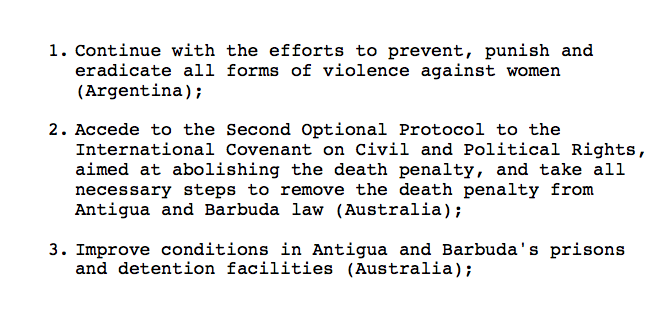
\includegraphics[width=0.7\linewidth]{img/upr-text} \end{center}

\textbf{The Task}: Parse a bunch of reports (PDFs) into a dataset (CSV).
Add metadata for issue, action, and sentiment.

\begin{center}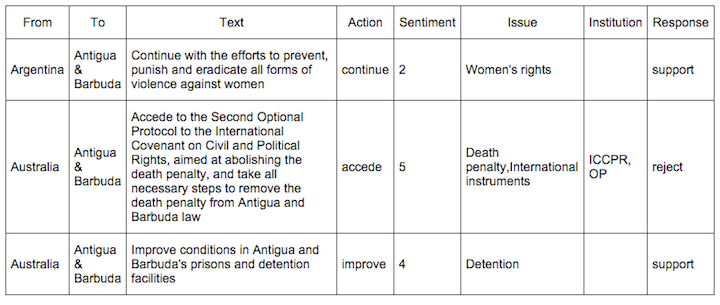
\includegraphics[width=0.7\linewidth]{img/upr-table} \end{center}

How much time will it take?

\textbf{By Hand}: 40,000 recommendations x 3 min per recommendation x
8-hour days x 5-day weeks = \textbf{12 months}

\subsubsection*{Task 2 (by hand)}\label{task-2-by-hand}
\addcontentsline{toc}{subsubsection}{Task 2 (by hand)}

What if we wanted to extend this research?

\textbf{Question:}: How does UPR shaming compare to actual human rights
abuses?

\textbf{Data}: Amnesty International's Urgent Actions

\textbf{Task}: Collect all of Amnesty International's Urgent Actions and
add metadata for issue and country.

\begin{center}
\includegraphics[width=0.7\linewidth]{img/amnesty} \end{center}

How much time will it take?

\textbf{By hand}: 25,000 recommendations x 3 min per recommendation x
8-hour days x 5-day weeks \textbf{= 7.5 months}

\subsubsection*{Tasks 1 \& 2 (with a
computer)}\label{tasks-1-2-with-a-computer}
\addcontentsline{toc}{subsubsection}{Tasks 1 \& 2 (with a computer)}

With a computer, we can write a program that

\begin{enumerate}
\def\labelenumi{\arabic{enumi}.}
\tightlist
\item
  Parses recommendations into a CSV.
\item
  Codes recommendations by issue, action, and sentiment using
  computational text analysis tools.
\item
  Uses webscraping to collect all of Amnesty International's urgent
  actions.
\item
  Runs simple regression models with R to correlate Amnesty reports with
  UPR shaming.
\end{enumerate}

Total time: 2 months

\textbf{Time Saved: 1.5 years}

\section{About This Class}\label{about-this-class}

\subsubsection*{About Me}\label{about-me}
\addcontentsline{toc}{subsubsection}{About Me}

My name is Rochelle Terman and I am a faculty member in Political
Science.

\begin{itemize}
\tightlist
\item
  A few years ago, I did not know how to program. Now I program almost
  every day.
\item
  I program mostly in Python and R. I have a special interest in text
  analysis and webscraping.
\item
  My substantive research is on international norms and human rights.
\item
  I will not be able to answer all your questions.
\item
  No one will.
\item
  But especially me.
\end{itemize}

\subsubsection*{Course Structure}\label{course-structure}
\addcontentsline{toc}{subsubsection}{Course Structure}

The course is divided into two main sections:

\textbf{1. Skills}

Basic computer literacy, terminologies, and programming languages:

\begin{itemize}
\tightlist
\item
  Base R: objects and data structures.
\item
  \texttt{tidyverse} for data analysis.
\item
  Modeling and visualization.
\item
  Key programming concepts (iteration, functions, conditional flow,
  etc.).
\end{itemize}

We are using R because it is the common programming language among
Political Scientists. But if you understand the \emph{concepts}, you
should able to pick up Python and other languages pretty easily.

\textbf{2. Applications}

Use the skills learned in part 1 towards practical applications:

\begin{itemize}
\tightlist
\item
  Webscraping.
\item
  APIs.
\item
  Computational Text Analysis.
\item
  Version control and communication.
\end{itemize}

The goal is to \textbf{introduce} the students to a medley of common
applications so that they can discover which avenue to pursue in their
own research and what such training would entail.

\subsubsection*{Class Activities}\label{class-activities}
\addcontentsline{toc}{subsubsection}{Class Activities}

Classes will follow a ``workshop'' style, combining lecture,
demonstration, and coding exercises. We envision the class to be as
interactive/hands-on as possible, with students programming every
session.

It is important that students \textbf{complete the requisite reading}
before class. I anticipate spending 1/2 the class lecturing and 1/2
practicing with coding challenges.

\subsubsection*{Course Websites}\label{course-websites}
\addcontentsline{toc}{subsubsection}{Course Websites}

Class notes and other materials are available here:
\url{https://github.com/plsc-31101/course/}

We will use Canvas to distribute/accept assignments.

We will use Piazza for communications and discussion. Please use Piazza
liberally.

\subsubsection*{Evaluation}\label{evaluation}
\addcontentsline{toc}{subsubsection}{Evaluation}

This is a graded class based on the following:

\begin{itemize}
\tightlist
\item
  Completion of assigned homework (50\%).
\item
  Participation (25\%).
\item
  Final project (25\%).
\end{itemize}

If you want to audit, please let me know ASAP.

\textbf{Assignments}

\begin{itemize}
\tightlist
\item
  In general, assignments are assigned at the end of lecture and are due
  the following week.
\item
  Exceptions will be noted.
\item
  The first assignment is due next week before class on Wednesday,
  October 7. It is available on Canvas.
\item
  Turn in assignments on Canvas.
\item
  Work in groups, but submit your own assignment.
\end{itemize}

\textbf{Participation}

The class participation portion of the grade can be satisfied in one or
more of the following ways:

\begin{itemize}
\tightlist
\item
  Attending the lectures.
\item
  Asking and answering questions in class.
\item
  Attending office hours.
\item
  Contributing to class discussion through the Piazza site.
\item
  Collaborating with the computing community.
\end{itemize}

\textbf{Final Project}

Students have two options for class projects:

\begin{enumerate}
\def\labelenumi{\arabic{enumi}.}
\item
  \textbf{Data project}: Use the tools we learned in class on your own
  data of interest.
\item
  \textbf{Tutorial project}: Create a tutorial on a tool we did not
  cover in class.
\end{enumerate}

Both options require an R Markdown file narrating the project.

Students are required to write a short proposal by \textbf{November 6}
(no more than 2 paragraphs) in order to get approval/feedback from the
instructors.

Project materials (i.e., a GitHub repo) will be due by end of day on
\textbf{December 10}. We will specify submission details in class.

On \textbf{December 11}, we will have a \textbf{lightning talk session}
where students can present their projects in a maximum 5-minute talk.

\subsubsection*{Software}\label{software}
\addcontentsline{toc}{subsubsection}{Software}

\begin{itemize}
\tightlist
\item
  Installation instructions are on the website.
\item
  Get started \textbf{EARLY}.
\item
  Go to the Installfest (Wednesday, Sep 30, 9:30-11:30 on Zoom) to
  double check your installation.
\item
  If you have computer troubles, post the problem on Piazza with as much
  detail as possible.
\end{itemize}

\section{Learning How to Program}\label{learning-how-to-program}

Before we talk about what it takes to learn how to program, let's first
review what programming is.

\subsubsection*{What is programming?}\label{what-is-programming}
\addcontentsline{toc}{subsubsection}{What is programming?}

A \emph{program} is a sequence of instructions that specifies how to
perform a computation. Most programs are written in a human-readable
\emph{programming language} (or ``source code'') and then executed with
the help of a \emph{compiler} or \emph{interpreter}.

A few basic instructions appear in just about every language:

\begin{enumerate}
\def\labelenumi{\arabic{enumi}.}
\tightlist
\item
  \textbf{Input}: Get data from the keyboard, a file, the network, or
  some other device.
\item
  \textbf{Output}: Display data on the screen, save it in a file, send
  it over the network, etc.
\item
  \textbf{Math}: Perform basic mathematical operations like addition and
  multiplication.
\item
  \textbf{Conditional execution}: Only perform tasks if certain
  conditions are met.
\item
  \textbf{Iteration}: Do the same task over and over again on different
  inputs.
\end{enumerate}

That being said, programming languages differ from one another in the
following ways:

\begin{enumerate}
\def\labelenumi{\arabic{enumi}.}
\tightlist
\item
  \textbf{Syntax}: Whether to add a semicolon at the end of each line,
  etc.
\item
  \textbf{Usage}: JavaScript is for building websites, R is for
  statistics, Python is general purpose, etc.
\item
  \textbf{Level}: How close you are to the hardware. `C' is often
  considered to be the lowest- (or one of the lowest-) level language.
\item
  \textbf{Object-oriented}: ``Objects'' are data + functions. Some
  programming languages are object-oriented (e.g., Python), and some are
  not (e.g., C).
\item
  \textbf{Many more}: Here is a
  \href{https://en.wikipedia.org/wiki/List_of_programming_languages_by_type}{list}
  of all the types of programming languages out there.
\end{enumerate}

\subsubsection*{What language should you
learn?}\label{what-language-should-you-learn}
\addcontentsline{toc}{subsubsection}{What language should you learn?}

Most programmers can program in more than one language. That is because
they know \emph{how to program} generally, as opposed to ``knowing''
Python, R, Ruby, or whatever.

So what should your first programming language be? That is, what
programming language should you use to learn \emph{how to program}? At
the end of the day, the answer depends on what you want to get out of
programming. Many people recommend Python because it is fun, easy, and
multi-purpose. Here is an
\href{http://lifehacker.com/which-programming-language-should-i-learn-first-1477153665}{article}
that can offer more advice.

In this class, we will be using R because it is the most popular
language in our disciplinary community (of political scientists).

Regardless of what you choose, you will probably grow comfortable in one
language while learning the basic concepts and skills that allow you to
`hack' your way into other languages. That is because
\textbf{programming is an extendible skill}.

Thus, ``knowing how to program'' means learning how to \emph{think} like
a programmer, not necessarily knowing all the language-specific commands
off the top of your head. \textbf{Do not learn specific programming
languages; learn how to program.}

\subsubsection*{What programming is really
like.}\label{what-programming-is-really-like.}
\addcontentsline{toc}{subsubsection}{What programming is really like.}

\begin{center}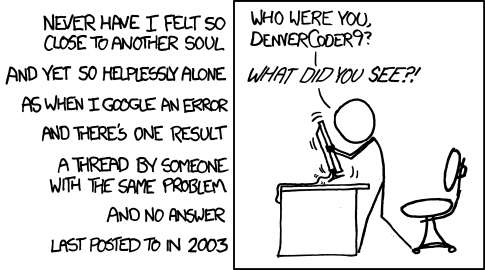
\includegraphics[width=0.7\linewidth]{img/xkcd} \end{center}

Here is the sad reality: When you are programming, 80\% or more of your
time will be spent debugging, looking stuff up (like program-specific
syntax, documentation for packages, useful functions, etc.), or testing.
This does not apply just to beginner or intermediate programmers,
although you will grow more ``fluent'' over time.

\begin{quote}
Google software engineers write an average of 10-20 lines of code per
day.
\end{quote}

\begin{quote}
\textbf{The lesson}: Programming is a slow activity, especially in the
beginning.
\end{quote}

If you are a good programmer, you are a good detective!

\subsubsection*{How to Learn}\label{how-to-learn}
\addcontentsline{toc}{subsubsection}{How to Learn}

Here are some tips on how to learn computer programming:

\begin{enumerate}
\def\labelenumi{\arabic{enumi}.}
\tightlist
\item
  Learning to program is 5\% intelligence, 95\% endurance.
\item
  Like learning to play an instrument or speak a foreign language, it
  takes practice, practice, practice.
\item
  Program a little bit every day.
\item
  Program with others. Do the problem sets in pairs or groups.
\item
  It is better to type than to copy and paste.
\item
  Most ``programming'' is actually researching, experimenting, and
  thinking.
\item
  Stay organized.
\end{enumerate}

\subsubsection*{The 15-Minute Rule}\label{the-15-minute-rule}
\addcontentsline{toc}{subsubsection}{The 15-Minute Rule}

15 min rule: when stuck, you HAVE to try on your own for 15 min; after
15 min, you HAVE to ask for help.- Brain AMA pic.twitter.com/MS7FnjXoGH

--- Rachel Thomas (\citet{math_rachel}) August 14, 2016

We will follow the \textbf{15-minute rule} in this class. If you
encounter a problem in your assignments, spend 15 minutes
troubleshooting the problem on your own. After 15 minutes, if you still
cannot solve the problem, \textbf{ask for help}.

(Hat tip to
\href{https://cfss.uchicago.edu/faq/asking-questions/}{Computing for
Social Sciences}.)

\subsubsection*{Debugging}\label{debugging}
\addcontentsline{toc}{subsubsection}{Debugging}

Those first 15 minutes should be spent trying to debug your code. Here
are some tips:

\begin{itemize}
\tightlist
\item
  Read the errors!
\item
  Read the documentation.
\item
  Make it smaller.
\item
  Figure out what changed.
\item
  Check your syntax.
\item
  Print statements are your friends.
\end{itemize}

\subsubsection*{Using the Internet}\label{using-the-internet}
\addcontentsline{toc}{subsubsection}{Using the Internet}

You should also make use of \href{https://www.google.com}{Google} and
\href{http://stackoverflow.com/}{StackOverflow} to resolve the error.
Here are some tips for how to google errors:

\begin{itemize}
\tightlist
\item
  Google: name-of-program + text in error message.
\item
  Remove user- and data-specific information first!
\item
  See if you can find examples that do and do not produce the error. Try
  other people's code, but do not fall into the copy-paste trap.
\end{itemize}

\subsubsection*{Asking for Help}\label{asking-for-help}
\addcontentsline{toc}{subsubsection}{Asking for Help}

We will use Piazza for class-related questions and discussion. You are
highly encouraged to ask questions and answer one another's questions.

\begin{enumerate}
\def\labelenumi{\arabic{enumi}.}
\tightlist
\item
  Include a brief, informative title.
\item
  Explain what you are trying to do and how it failed.
\item
  Include a reproducible example.
\end{enumerate}

Here are some helpful guidelines on how to properly ask programming
questions:

\begin{enumerate}
\def\labelenumi{\arabic{enumi}.}
\tightlist
\item
  \href{https://www.propublica.org/nerds/how-to-ask-programming-questions}{``How
  to Ask Programming Questions,'' ProPublica.}
\item
  \href{https://stackoverflow.com/help/how-to-ask}{``How do I ask a good
  question?'' StackOverflow.}
\item
  \href{https://cfss.uchicago.edu/faq/asking-questions/}{``How to
  properly ask for help,'' Computing for Social Science.}
\end{enumerate}

\chapter{R Basics}\label{r-basics}

This unit introduces you to the R programming language and the tools we
use to program in R. We will explore:

\begin{enumerate}
\def\labelenumi{\arabic{enumi}.}
\tightlist
\item
  \textbf{\protect\hyperlink{what-is-r}{What is R?}}, a brief
  introduction to the R language.
\item
  \textbf{\protect\hyperlink{rstudio-1}{RStudio}}, a tour of the
  Interactive Development Environment RStudio.
\item
  \textbf{\protect\hyperlink{r-packages-1}{R Packages}}, extra tools and
  functionalities.
\item
  \textbf{\protect\hyperlink{r-markdown}{R Markdown}}, a type of R
  script file we will be working with in this class.
\end{enumerate}

\hypertarget{what-is-r}{\section{What is R?}\label{what-is-r}}

R is a versatile, open-source programming and scripting language that is
useful both for statistics and data science. It is inspired by the
programming language
\href{https://en.wikipedia.org/wiki/S_(programming_language)}{S}. Some
of its \textbf{best features} are:

\begin{itemize}
\item
  It is free, open-source, and available on every major platform. As a
  result, if you do your analysis in R, most people can easily replicate
  it.
\item
  It contains a massive set of packages for statistical modelling,
  machine learning, visualization, and importing and manipulating data.
  Over 14,000 packages are available as of August 2019. Whatever model
  or graphic you are trying to do, chances are that someone has already
  tried to do it (and a package for it exists).
\item
  It is designed for statistics and data analysis, but also
  general-purpose programming.
\item
  It is an \href{http://www.rstudio.com/ide/}{Interactive Development
  Environment} tailored to the needs of interactive data analysis and
  statistical programming.
\item
  It has powerful tools for communicating your results. R packages make
  it easy to produce HTML or PDF
  \href{http://yihui.name/knitr/}{reports}, or create
  \href{http://www.rstudio.com/shiny/}{interactive websites}.
\item
  A large and growing community of peers.
\end{itemize}

R also has a number of \textbf{shortcomings}:

\begin{itemize}
\item
  It has a steeper learning curve than SPSS or Stata.
\item
  R is not a particularly fast programming language, and poorly written
  R code can be terribly slow. R is also a profligate user of memory.
\item
  Much of the R code you will see in the wild is written in haste to
  solve a pressing problem. As a result, code is not very elegant, fast,
  or easy to understand. Most users do not revise their code to address
  these shortcomings.
\item
  Inconsistency is rife across contributed packages, even within base R.
  You are confronted with over 20 years of evolution every time you use
  R. Learning R can be tough, because there are many special cases to
  remember.
\end{itemize}

\hypertarget{rstudio-1}{\section{RStudio}\label{rstudio-1}}

Throughout this class, we will assume that you are using R via RStudio.
First-time users often confuse the two. At its simplest, R is like a
car's engine, while RStudio is like a car's dashboard.

\begin{center}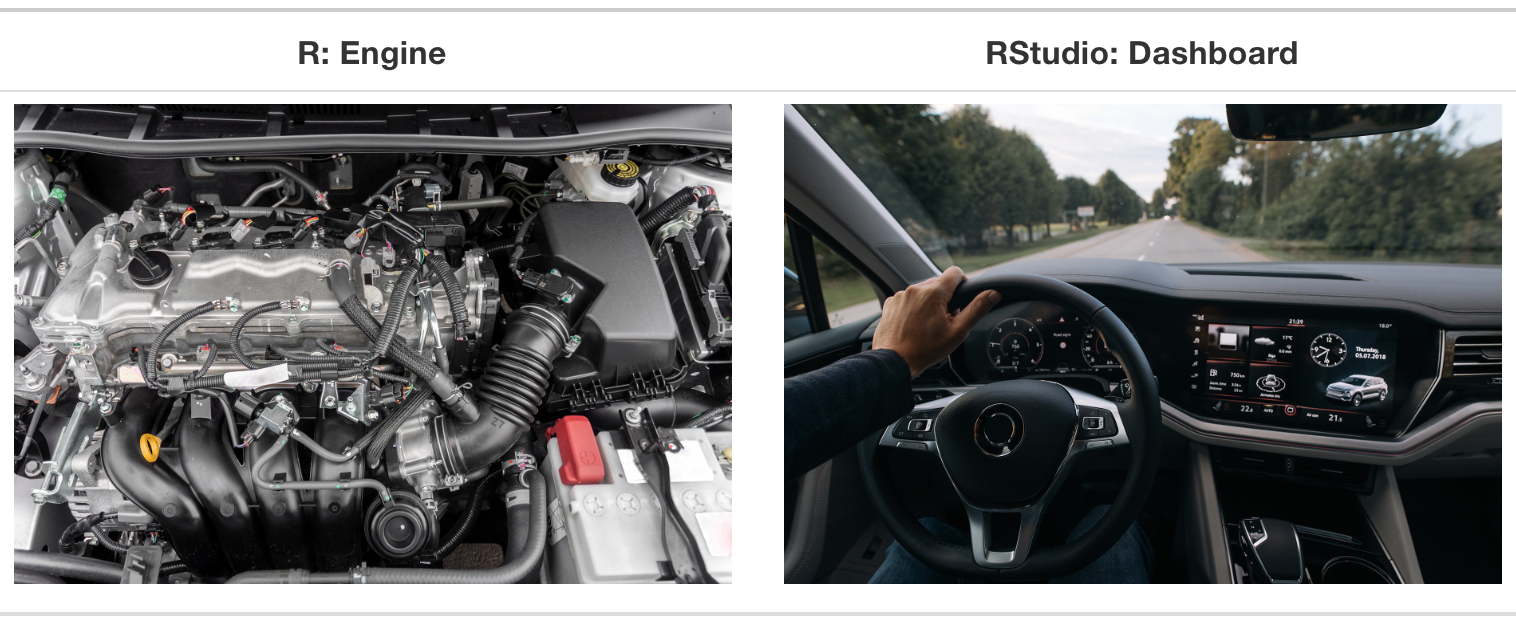
\includegraphics[width=0.7\linewidth]{img/R_vs_RStudio_1} \end{center}

More precisely, R is a programming language that runs computations,
while RStudio is an \emph{integrated development environment (IDE)} that
provides an interface with many convenient features and tools. Just as
the way of having access to a speedometer, rear-view mirrors, and a
navigation system makes driving much easier, using RStudio's interface
makes using R much easier as well.

RStudio includes a console, a syntax-highlighting code editor, as well
as tools for plotting, history, debuggingm and workspace management. It
is also free and open-source. Yay!

\textbf{NB}: We do not have to use RStudio to use R. For example, we can
write R code in a plain text editor (like \texttt{textedit} or
\texttt{notepad}) and then execute the script using the shell (e.g.,
\texttt{terminal} in Mac). But this is not ideal.

After you install R and RStudio on your computer, you will have two new
applications you can open. We will always work in RStudio -- not in the
R application.

\begin{center}
\includegraphics[width=0.7\linewidth]{img/R_vs_RStudio} \end{center}

After you open RStudio, you should see something similar to this:

\begin{center}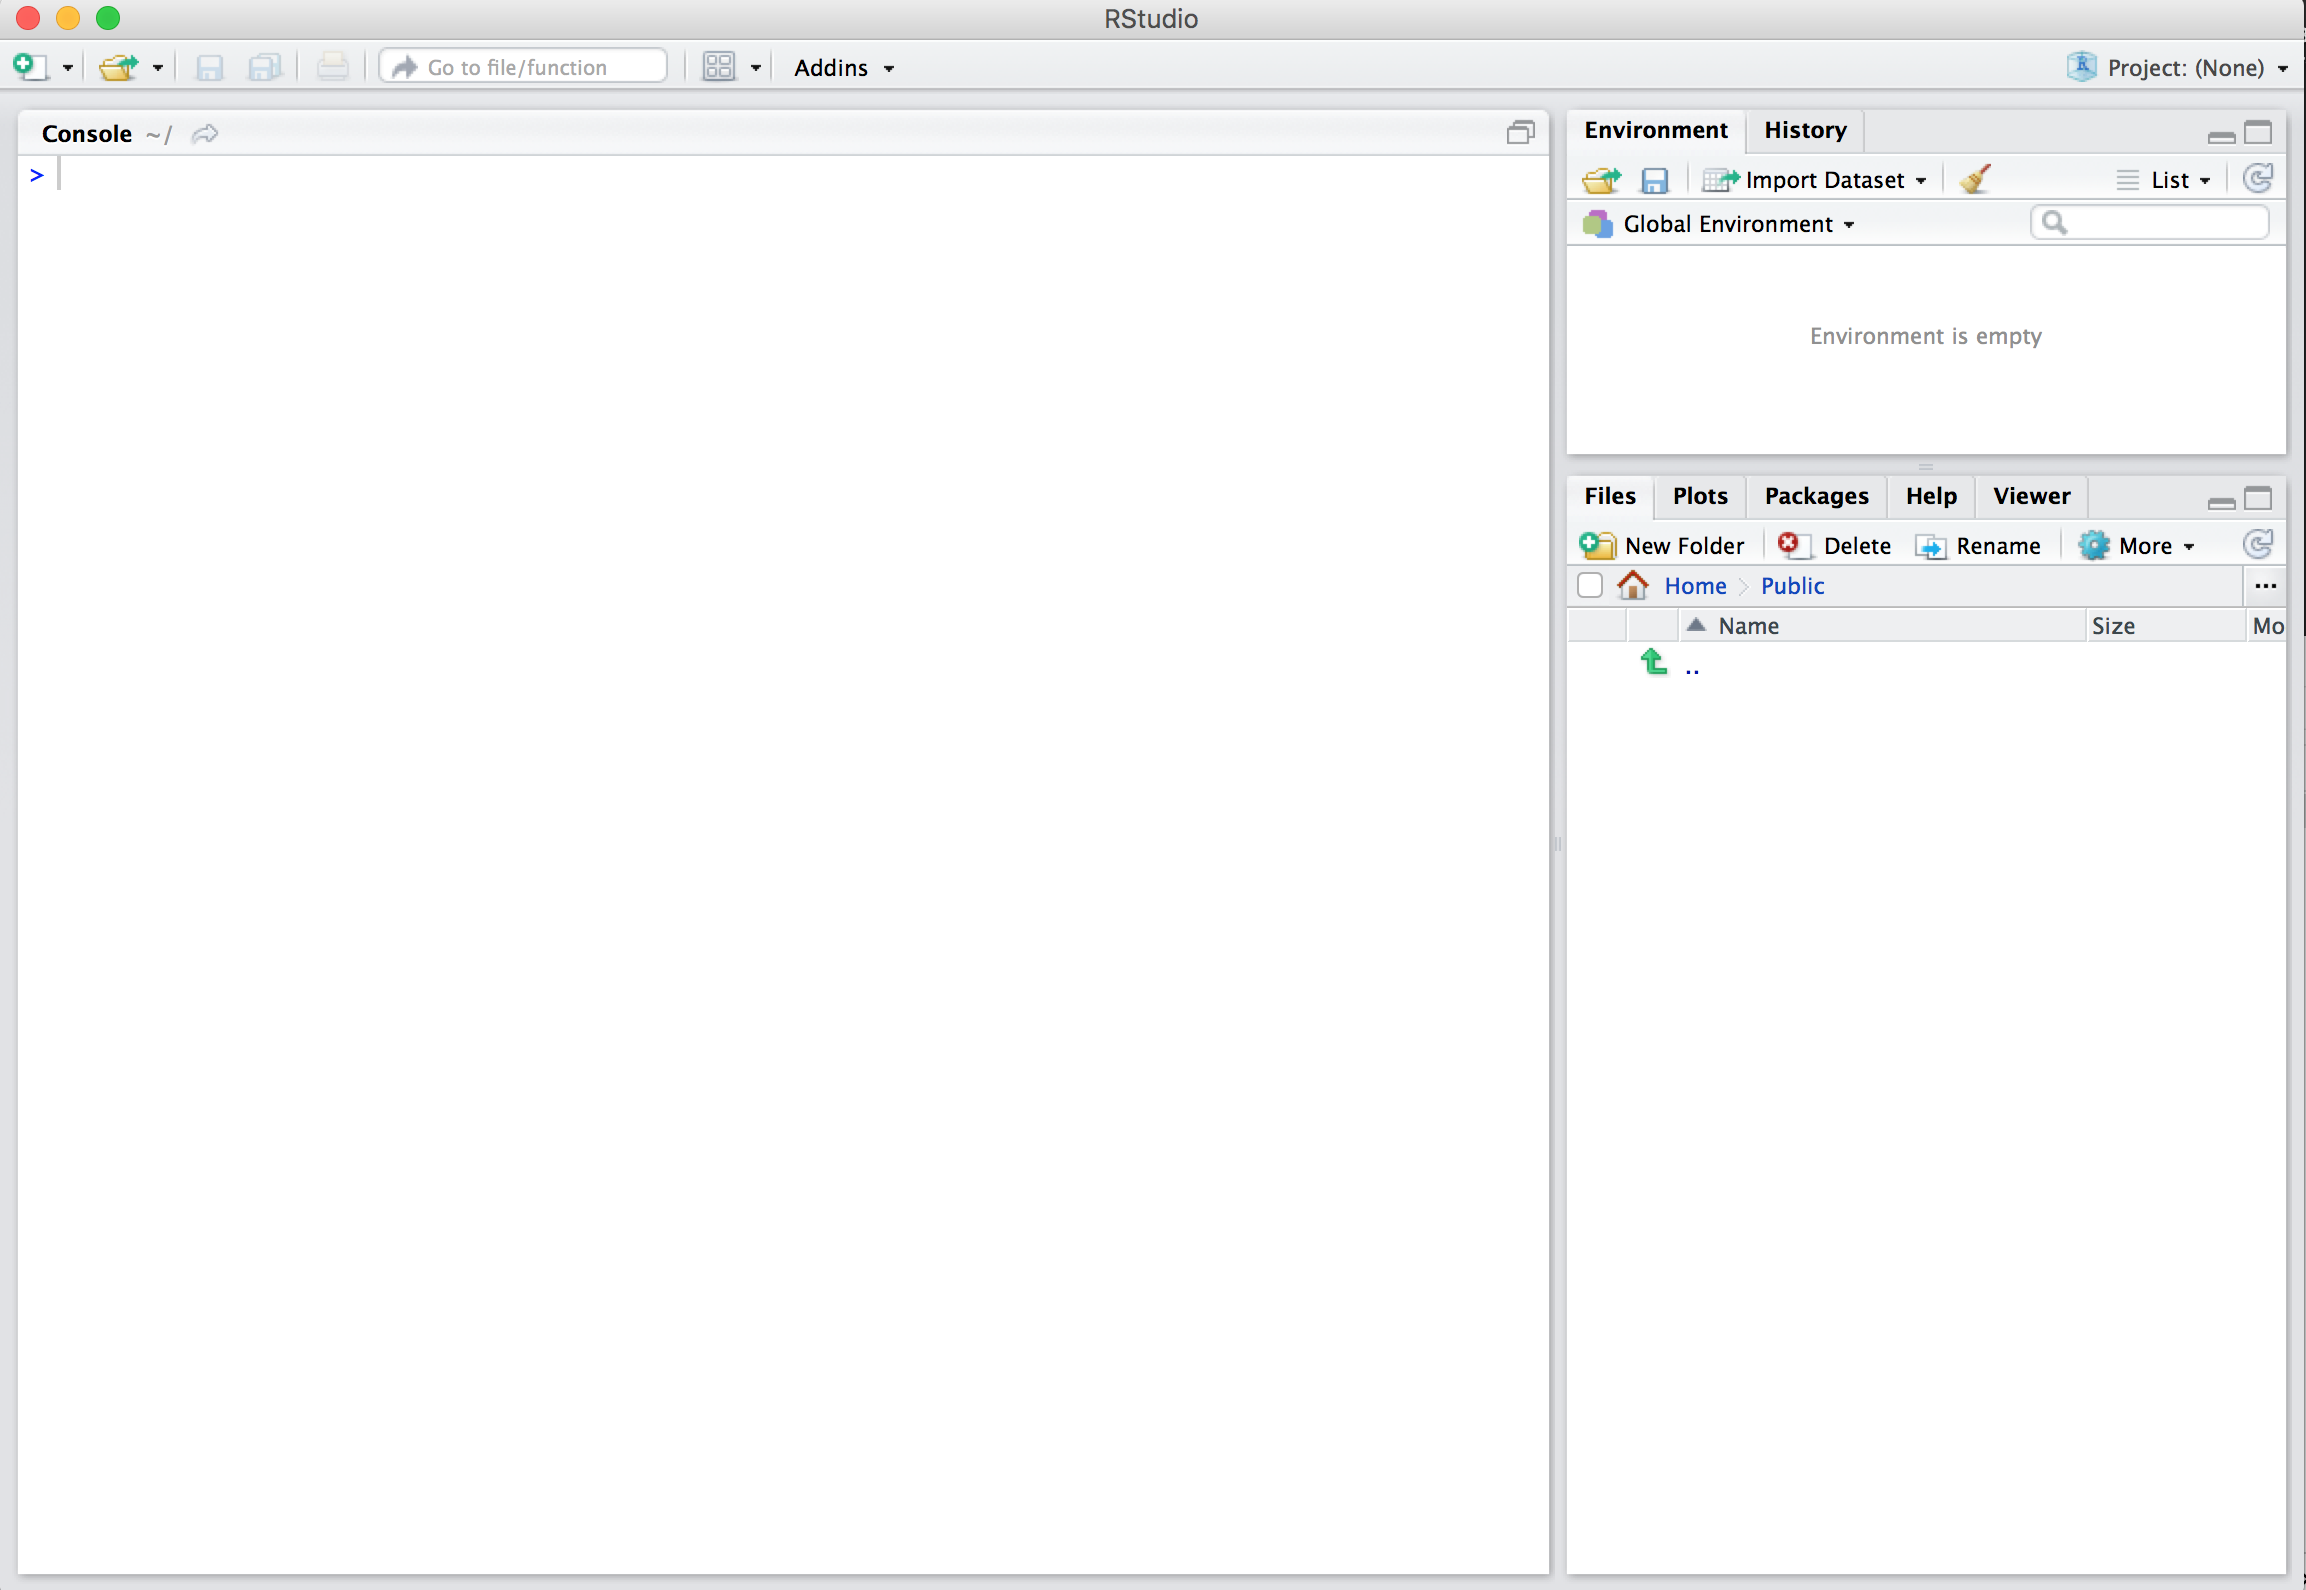
\includegraphics[width=0.7\linewidth]{img/rstudio} \end{center}

\subsection{Console}\label{console}

There are two main ways of interacting with R: by using the
\textbf{console} or by using the \textbf{script editor}.

The console window (in RStudio, the bottom left panel) is the place
where R is waiting for you to tell it what to do and where it will show
the results of a command.

You can type commands directly into the console, but they will be
forgotten when you close the session. Try it out now.

\begin{Shaded}
\begin{Highlighting}[]
\OperatorTok{>}\StringTok{ }\DecValTok{2} \OperatorTok{+}\StringTok{ }\DecValTok{2}
\end{Highlighting}
\end{Shaded}

If R is ready to accept commands, the R console shows a
\texttt{\textgreater{}} prompt. If it receives a command (by typing,
copy-pasting, or sending from the script editor using
\texttt{Ctrl-Enter}), R will try to execute it andm when ready, show the
results and come back with a new \texttt{\textgreater{}}-prompt to wait
for new commands.

If R is still waiting for you to enter more data because it is not
complete yet, the console will show a \texttt{+} prompt. It means that
you have not finished entering a complete command. This happens when you
have not `closed' a parenthesis or quotation. If you are in RStudio and
this happens, click inside the console window and press \texttt{Esc};
this should help get you out of trouble.

\begin{Shaded}
\begin{Highlighting}[]
\OperatorTok{>}\StringTok{ "This is an incomplete quote}
\StringTok{+}
\end{Highlighting}
\end{Shaded}

\subsubsection*{More Console Features}\label{more-console-features}
\addcontentsline{toc}{subsubsection}{More Console Features}

\begin{enumerate}
\def\labelenumi{\arabic{enumi}.}
\item
  Retrieving previous commands: As you work with R, you will often want
  to re-execute a command which you previously entered. Recall previous
  commands using the up and down arrow keys.
\item
  Console title bar: This screenshot illustrates a few additional
  capabilities provided by the console title bar:

  \begin{itemize}
  \tightlist
  \item
    Display of the current working directory.
  \item
    The ability to interrupt R during a long computation.
  \item
    Minimizing and maximizing the console in relation to the Source pane
    (by using the buttons at the top-right or by double-clicking the
    title bar).
  \end{itemize}
\end{enumerate}

\begin{center}
\includegraphics[width=0.7\linewidth]{img/using_console_title_bar} \end{center}

\subsection{Scripts}\label{scripts}

It is better practice to enter commands in the script editor and save
the script. This way, you have a complete record of what you did, you
can easily show others how you did it, and you can do it again later on
if needed. Open it up either by clicking the \emph{File} menu and
selecting \emph{New File}, then R script; or by using the keyboard
shortcut Cmd/Ctrl + Shift + N. Now you will see four panes.

\begin{center}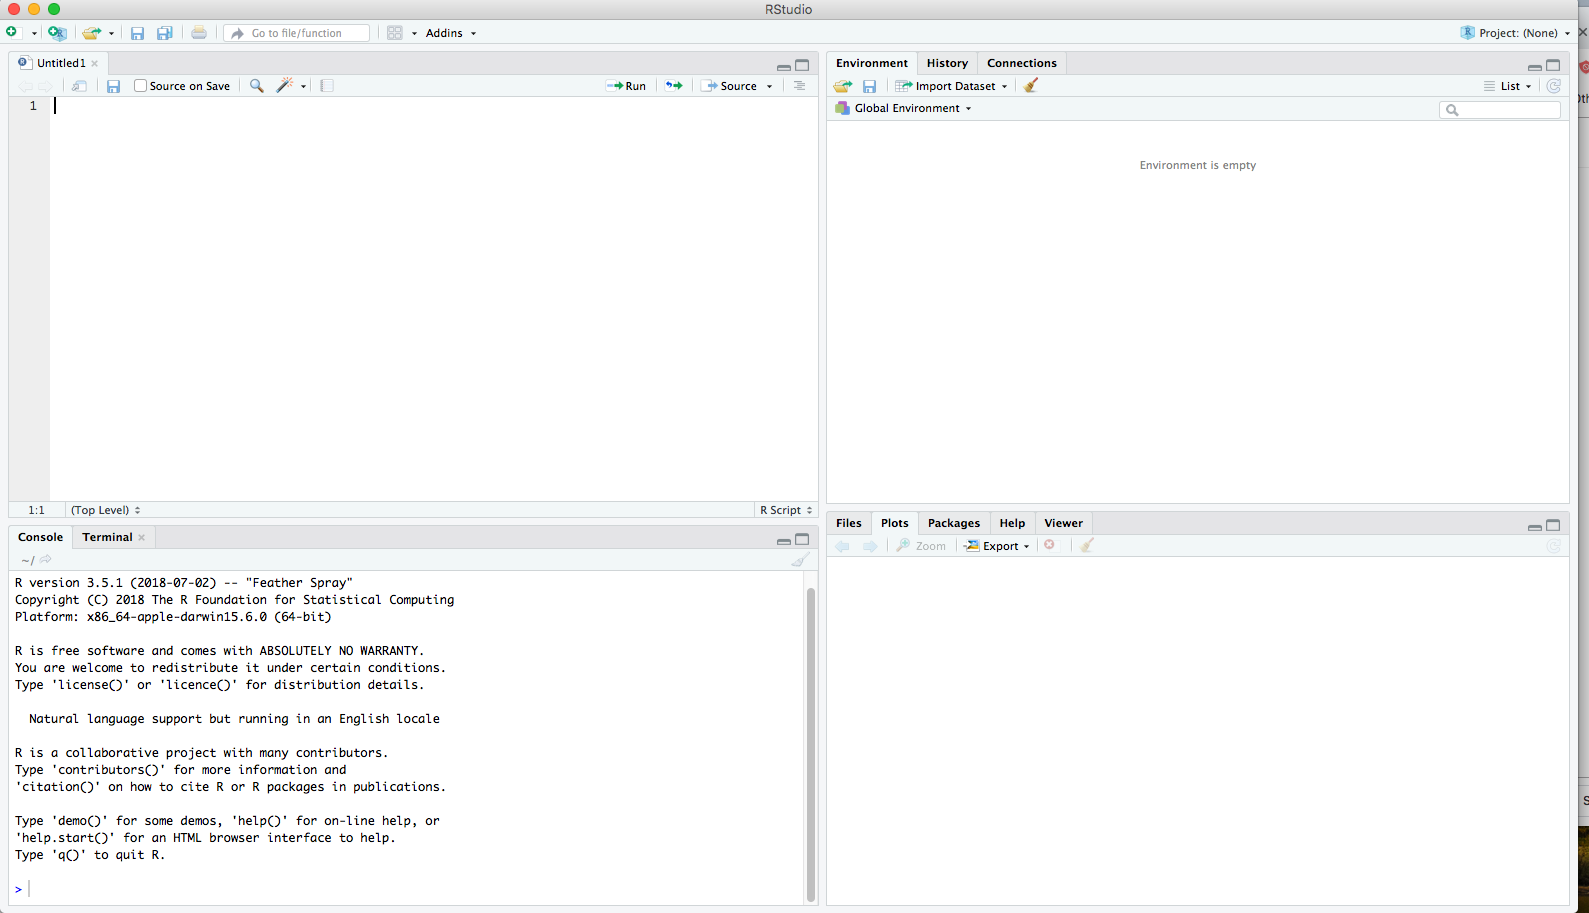
\includegraphics[width=0.7\linewidth]{img/4-panes} \end{center}

The script editor is a great place to put code you care about. Keep
experimenting in the console, but, once you have written code that works
and does what you want, put it in the script editor.

RStudio will automatically save the contents of the editor when you quit
RStudio and load them when you re-open RStudio. Nevertheless, it is a
good idea to save your scripts regularly and to back them up.

\subsection{Running Code}\label{running-code}

While you certainly can copy-paste code that you would like to run from
the editor into the console, this workflow is pretty inefficient. The
key to using the script editor effectively is to memorize one of the
most important keyboard shortcuts in RStudio:
\textbf{\texttt{Cmd/Ctrl\ +\ Enter}}. This executes the current R
expression from the script editor in the console.

For example, take the code below. If your cursor is somewhere on the
first line, pressing \texttt{Cmd/Ctrl\ +\ Enter} will run the complete
command that generates \texttt{dems}. It will also move the cursor to
the next statement (beginning with \texttt{reps}). That makes it easy to
run your complete script by repeatedly pressing
\texttt{Cmd/Ctrl\ +\ Enter}.

\begin{Shaded}
\begin{Highlighting}[]
\NormalTok{dems <-}\StringTok{ }\NormalTok{(}\DecValTok{55} \OperatorTok{+}\StringTok{ }\DecValTok{70}\NormalTok{) }\OperatorTok{*}\StringTok{ }\FloatTok{1.3}

\NormalTok{reps <-}\StringTok{ }\NormalTok{(}\DecValTok{20} \OperatorTok{-}\StringTok{ }\DecValTok{1}\NormalTok{) }\OperatorTok{/}\StringTok{ }\DecValTok{2}
\end{Highlighting}
\end{Shaded}

Instead of running expression by expression, you can also execute the
complete script in one step: \texttt{Cmd/Ctrl\ +\ Shift\ +\ Enter}.
Doing this regularly is a great way to check that you have captured all
the important parts of your code in the script.

\subsection{Comments}\label{comments}

Use \texttt{\#} signs to add comments within your code chunks. You are
encouraged to regularly comment within your code. Anything to the right
of a \texttt{\#} is ignored by R. Each line of a comment needs to begin
with a \texttt{\#}.

\begin{Shaded}
\begin{Highlighting}[]
\CommentTok{# This is a comment.}
\CommentTok{# This is another line of comments.}
\end{Highlighting}
\end{Shaded}

\subsection{Diagnostics and errors}\label{diagnostics-and-errors}

The script editor will also highlight syntax errors with a red squiggly
line and a cross in the sidebar:

\begin{center}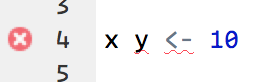
\includegraphics[width=0.7\linewidth]{img/rstudio-diagnostic} \end{center}

You can hover over the cross to see what the problem is:

\begin{center}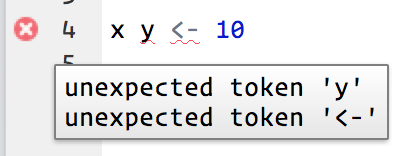
\includegraphics[width=0.7\linewidth]{img/rstudio-diagnostic-tip} \end{center}

If you try to execute the code, you will see an error in the console:

\begin{center}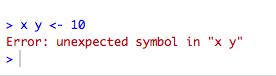
\includegraphics[width=0.7\linewidth]{img/error} \end{center}

When errors happen, your code is haulted -- meaning it is never
executed. Errors can be frustrating in R, but, with practice, you will
be able to debug your code quickly.

\subsection{Errors, Messages, and
Warnings}\label{errors-messages-and-warnings}

One thing that intimidates new R and RStudio users is how it reports
errors, warnings, and messages. R reports errors, warnings, and messages
in a glaring font, which makes it seem like it is scolding you. However,
seeing red text in the console is not always bad:

\begin{enumerate}
\def\labelenumi{\arabic{enumi}.}
\item
  \textbf{Errors}: When the text is a legitimate error, it will be
  prefaced with ``Error:'', and R will try to explain what went wrong.
  Generally, when there is an error, the code will not run. \emph{Think
  of errors as a red traffic light: something is wrong!}
\item
  \textbf{Warnings}: When the text is a warning, it will be prefaced
  with ``Warning:'', and R will try to explain why there is a warning.
  Generally, your code will still work, but perhaps not in the way you
  would expect. \emph{Think of warnings as a yellow traffic light:
  everything is working fine, but watch out/pay attention.}
\item
  \textbf{Messages}: When the text doesn not start with either
  ``Error:'' or ``Warning:'', it is just a friendly message. These are
  helpful diagnostic messages and they do not stop your code from
  working. \emph{Think of messages as a green traffic light: everything
  is working fine, and keep on going!}
\end{enumerate}

\subsection{R Environment}\label{r-environment}

Turn your attention to the upper right pane. This pane displays your
``global environment'' and contains the data objects you have saved in
your current session. Notice that we have the two objects created
earlier, \texttt{dems} and \texttt{reps}, along with their values.

You can list all objects in your current environment by running:

\begin{Shaded}
\begin{Highlighting}[]
\KeywordTok{ls}\NormalTok{()}
\CommentTok{#> [1] "dems" "reps"}
\end{Highlighting}
\end{Shaded}

Sometimes we want to remove objects that we no longer need.

\begin{Shaded}
\begin{Highlighting}[]
\NormalTok{x <-}\StringTok{ }\DecValTok{5}
\KeywordTok{rm}\NormalTok{(x)}
\end{Highlighting}
\end{Shaded}

If you want to remove all objects from your current environment, you can
run:

\begin{Shaded}
\begin{Highlighting}[]
\KeywordTok{rm}\NormalTok{(}\DataTypeTok{list =} \KeywordTok{ls}\NormalTok{())}
\end{Highlighting}
\end{Shaded}

\hypertarget{r-packages-1}{\section{R Packages}\label{r-packages-1}}

The best part about R are its user-contributed packages (also called
``libraries''). A \emph{package} is a collection of functions (and
sometimes data) that can be used by other programers.

A good analogy for R packages is they are like apps you can download
onto a mobile phone:

\begin{center}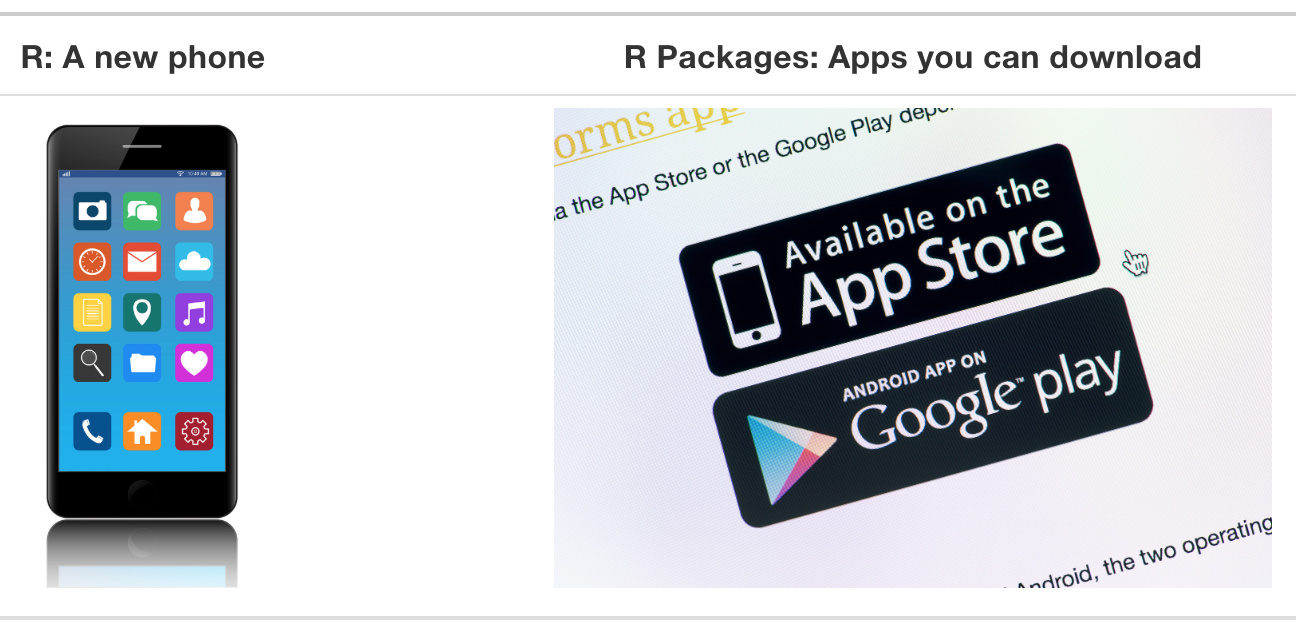
\includegraphics[width=0.7\linewidth]{img/R_vs_R_packages} \end{center}

So R is like a new mobile phone: while it has a certain amount of
features when you use it for the first time, it does not have
everything. R packages are like the apps you can download onto your
phone from Apple's App Store or Android's Google Play.

Let's continue this analogy by considering the Instagram app for editing
and sharing pictures. Say you have purchased a new phone and you would
like to share a photo you have just taken with friends and family on
Instagram. You need to:

\begin{enumerate}
\def\labelenumi{\arabic{enumi}.}
\tightlist
\item
  \textbf{Install the app}: Since your phone is new and does not include
  the Instagram app, you need to download the app from either the App
  Store or Google Play. You do this once and you are set for the time
  being. You might need to do this again in the future when there is an
  update to the app.
\item
  \textbf{Open the app}: After you have installed Instagram, you need to
  open the app.
\end{enumerate}

The process is very similar for using an R package. You need to:

\begin{enumerate}
\def\labelenumi{\arabic{enumi}.}
\tightlist
\item
  \textbf{Install the package}: This is like installing an app on your
  phone. Most packages are not installed by default when you install R
  and RStudio. Thus, if you want to use a package for the first time,
  you need to install it first. Once you have installed a package, you
  likely will not install it again unless you want to update it to a
  newer version.
\item
  \textbf{``Load'' the package}: Loading a package is like opening an
  app on your phone. Packages are not loaded by default when you start
  RStudio on your computer; you need to load each package you want to
  use every time you start RStudio.
\end{enumerate}

\subsection{Installing Packages}\label{installing-packages}

First, we download the package from one of the CRAN mirrors onto our
computer. For this we use \texttt{install.packages("package-name")}. If
you have not set a preferred CRAN mirror in your \texttt{options()}, a
menu will pop up asking you to choose a location.

Let's download the package \texttt{dplyr}.

\begin{Shaded}
\begin{Highlighting}[]
\KeywordTok{install.packages}\NormalTok{(}\StringTok{"dplyr"}\NormalTok{)}
\end{Highlighting}
\end{Shaded}

If you run into errors later in the course about a function or package
not being found, run the \texttt{install.packages} function to make sure
the package is actually installed.

\textbf{Important}: Once we download the package, we never need to run
\texttt{install.packages} again (unless we get a new computer).

\subsection{Loading Packages}\label{loading-packages}

Once we download the package, we need to load it into our session to use
it. This is required at the beginning of each R session. This step is
necessary because, if we automatically loaded every package we have ever
downloaded, our computer would fry.

\begin{Shaded}
\begin{Highlighting}[]
\KeywordTok{library}\NormalTok{(dplyr)}
\end{Highlighting}
\end{Shaded}

The message tells you which functions from \texttt{dplyr} conflict with
functions in base R (or from other packages you might have loaded).

\subsection{Challenge}\label{challenge}

Let's go ahead and download some core, important packages we will use
for the rest of the course. Download (if you have not done so already)
and load the following packages:

\begin{itemize}
\tightlist
\item
  \texttt{tidyverse}
\item
  \texttt{rmarkdown}
\item
  \texttt{knitr}
\item
  \texttt{gapminder}
\item
  \texttt{devtools}
\item
  \texttt{stargazer}
\item
  \texttt{rtweet}
\end{itemize}

\hypertarget{r-markdown}{\section{R Markdown}\label{r-markdown}}

Throughout this course, we will be using
\href{http://rmarkdown.rstudio.com\%3E}{R Markdown} for lecture notes
and homework assignments. R Markdown documents combine executable code,
results, and prose commentary into one document. Think of an R Markdown
files as a modern-day lab notebook, where you can capture not only what
you did, but also what you were thinking.

The filename of an R Markdown document should end in \texttt{.Rmd} or
\texttt{.rmd}. An R Markdown document can also be converted to an output
format, like PDF, HTML, slideshows, Word files, and more.

R Markdown documents contain three important types of content:

\begin{enumerate}
\def\labelenumi{\arabic{enumi}.}
\tightlist
\item
  An (optional) YAML header surrounded by \texttt{-\/-\/-}s.
\item
  Chunks of R code surrounded by
  \texttt{\textasciigrave{}\textasciigrave{}\textasciigrave{}}.
\item
  Text mixed with simple text formatting like \texttt{\#\ heading} and
  \texttt{\_italics\_}.
\end{enumerate}

\subsection{YAML Header}\label{yaml-header}

YAML stands for ``yet another markup language.'' R Markdown uses it to
control many details of the output.

\begin{Shaded}
\begin{Highlighting}[]
\NormalTok{---}
\NormalTok{title: "Homework 1"}
\NormalTok{author: "Rochelle Terman"}
\NormalTok{date: "Fall 2020"}
\NormalTok{output: html_document}
\NormalTok{---}
\end{Highlighting}
\end{Shaded}

In this example, we specified the document's title, author, and date; we
also specified that we want it to eventually be converted into an HTML
document.

\subsection{Markdown}\label{markdown}

Prose in \texttt{.Rmd} files is written in Markdown, a lightweight set
of conventions for formatting plain text files. Markdown is designed to
be easy to read and easy to write. It is also very easy to learn. The
guide below shows how to use Pandoc's Markdown, a slightly extended
version of Markdown that R Markdown understands.

\begin{Shaded}
\begin{Highlighting}[]
\NormalTok{Text formatting }
\NormalTok{------------------------------------------------------------}

\NormalTok{*italic*  or _italic_}
\NormalTok{**bold**   __bold__}
\BaseNTok{`code`}
\NormalTok{superscript^2^ and subscript~2~}

\NormalTok{Headings}
\NormalTok{------------------------------------------------------------}

\FunctionTok{# 1st Level Header}

\FunctionTok{## 2nd Level Header}

\FunctionTok{### 3rd Level Header}

\NormalTok{Lists}
\NormalTok{------------------------------------------------------------}

\NormalTok{* }\FloatTok{  Bulleted list item 1}

\NormalTok{* }\FloatTok{  Item 2}

\BaseNTok{    * Item 2a}

\BaseNTok{    * Item 2b}

\NormalTok{1. }\FloatTok{ Numbered list item 1}

\NormalTok{1. }\FloatTok{ Item 2. The numbers are incremented automatically in the output.}

\NormalTok{Links and images}
\NormalTok{------------------------------------------------------------}

\OtherTok{<http://example.com>}

\OtherTok{[linked phrase](http://example.com)}

\AlertTok{![optional caption text](path/to/img.png)}

\NormalTok{Tables }
\NormalTok{------------------------------------------------------------}

\NormalTok{First Header  | Second Header}
\NormalTok{------------- | -------------}
\NormalTok{Content Cell  | Content Cell}
\NormalTok{Content Cell  | Content Cell}
\end{Highlighting}
\end{Shaded}

The best way to learn these is simply to try them out. It will take a
few days, but soon they will become second nature, and you will not need
to think about them. If you forget, you can get to a handy reference
sheet with Help \textgreater{} Markdown Quick Reference.

\subsection{Code Chunks}\label{code-chunks}

To run code inside an R Markdown document, you do it inside a ``chunk.''
Think of a chunk like a step in a larger process. A chunk should be
relatively self-contained and focused around a single task.

Chunks begin with a header which consists of
\texttt{\textasciigrave{}\textasciigrave{}\textasciigrave{}\{r,},
followed by an optional chunk name, followed by comma separated options,
followed by \texttt{\}}. Next comes your R code, and the chunk end is
indicated by a final
\texttt{\textasciigrave{}\textasciigrave{}\textasciigrave{}}.

You can continue to run the code using the keyboard shortcut that we
learned earlier: \texttt{Cmd/Ctrl\ +\ Enter}. You can also run the
entire chunk by clicking the Run icon (it looks like a play button at
the top of the chunk) or by pressing
\texttt{Cmd/Ctrl\ +\ Shift\ +\ Enter}.

RStudio executes the code and displays the results inline with the code:

\begin{figure}
\centering
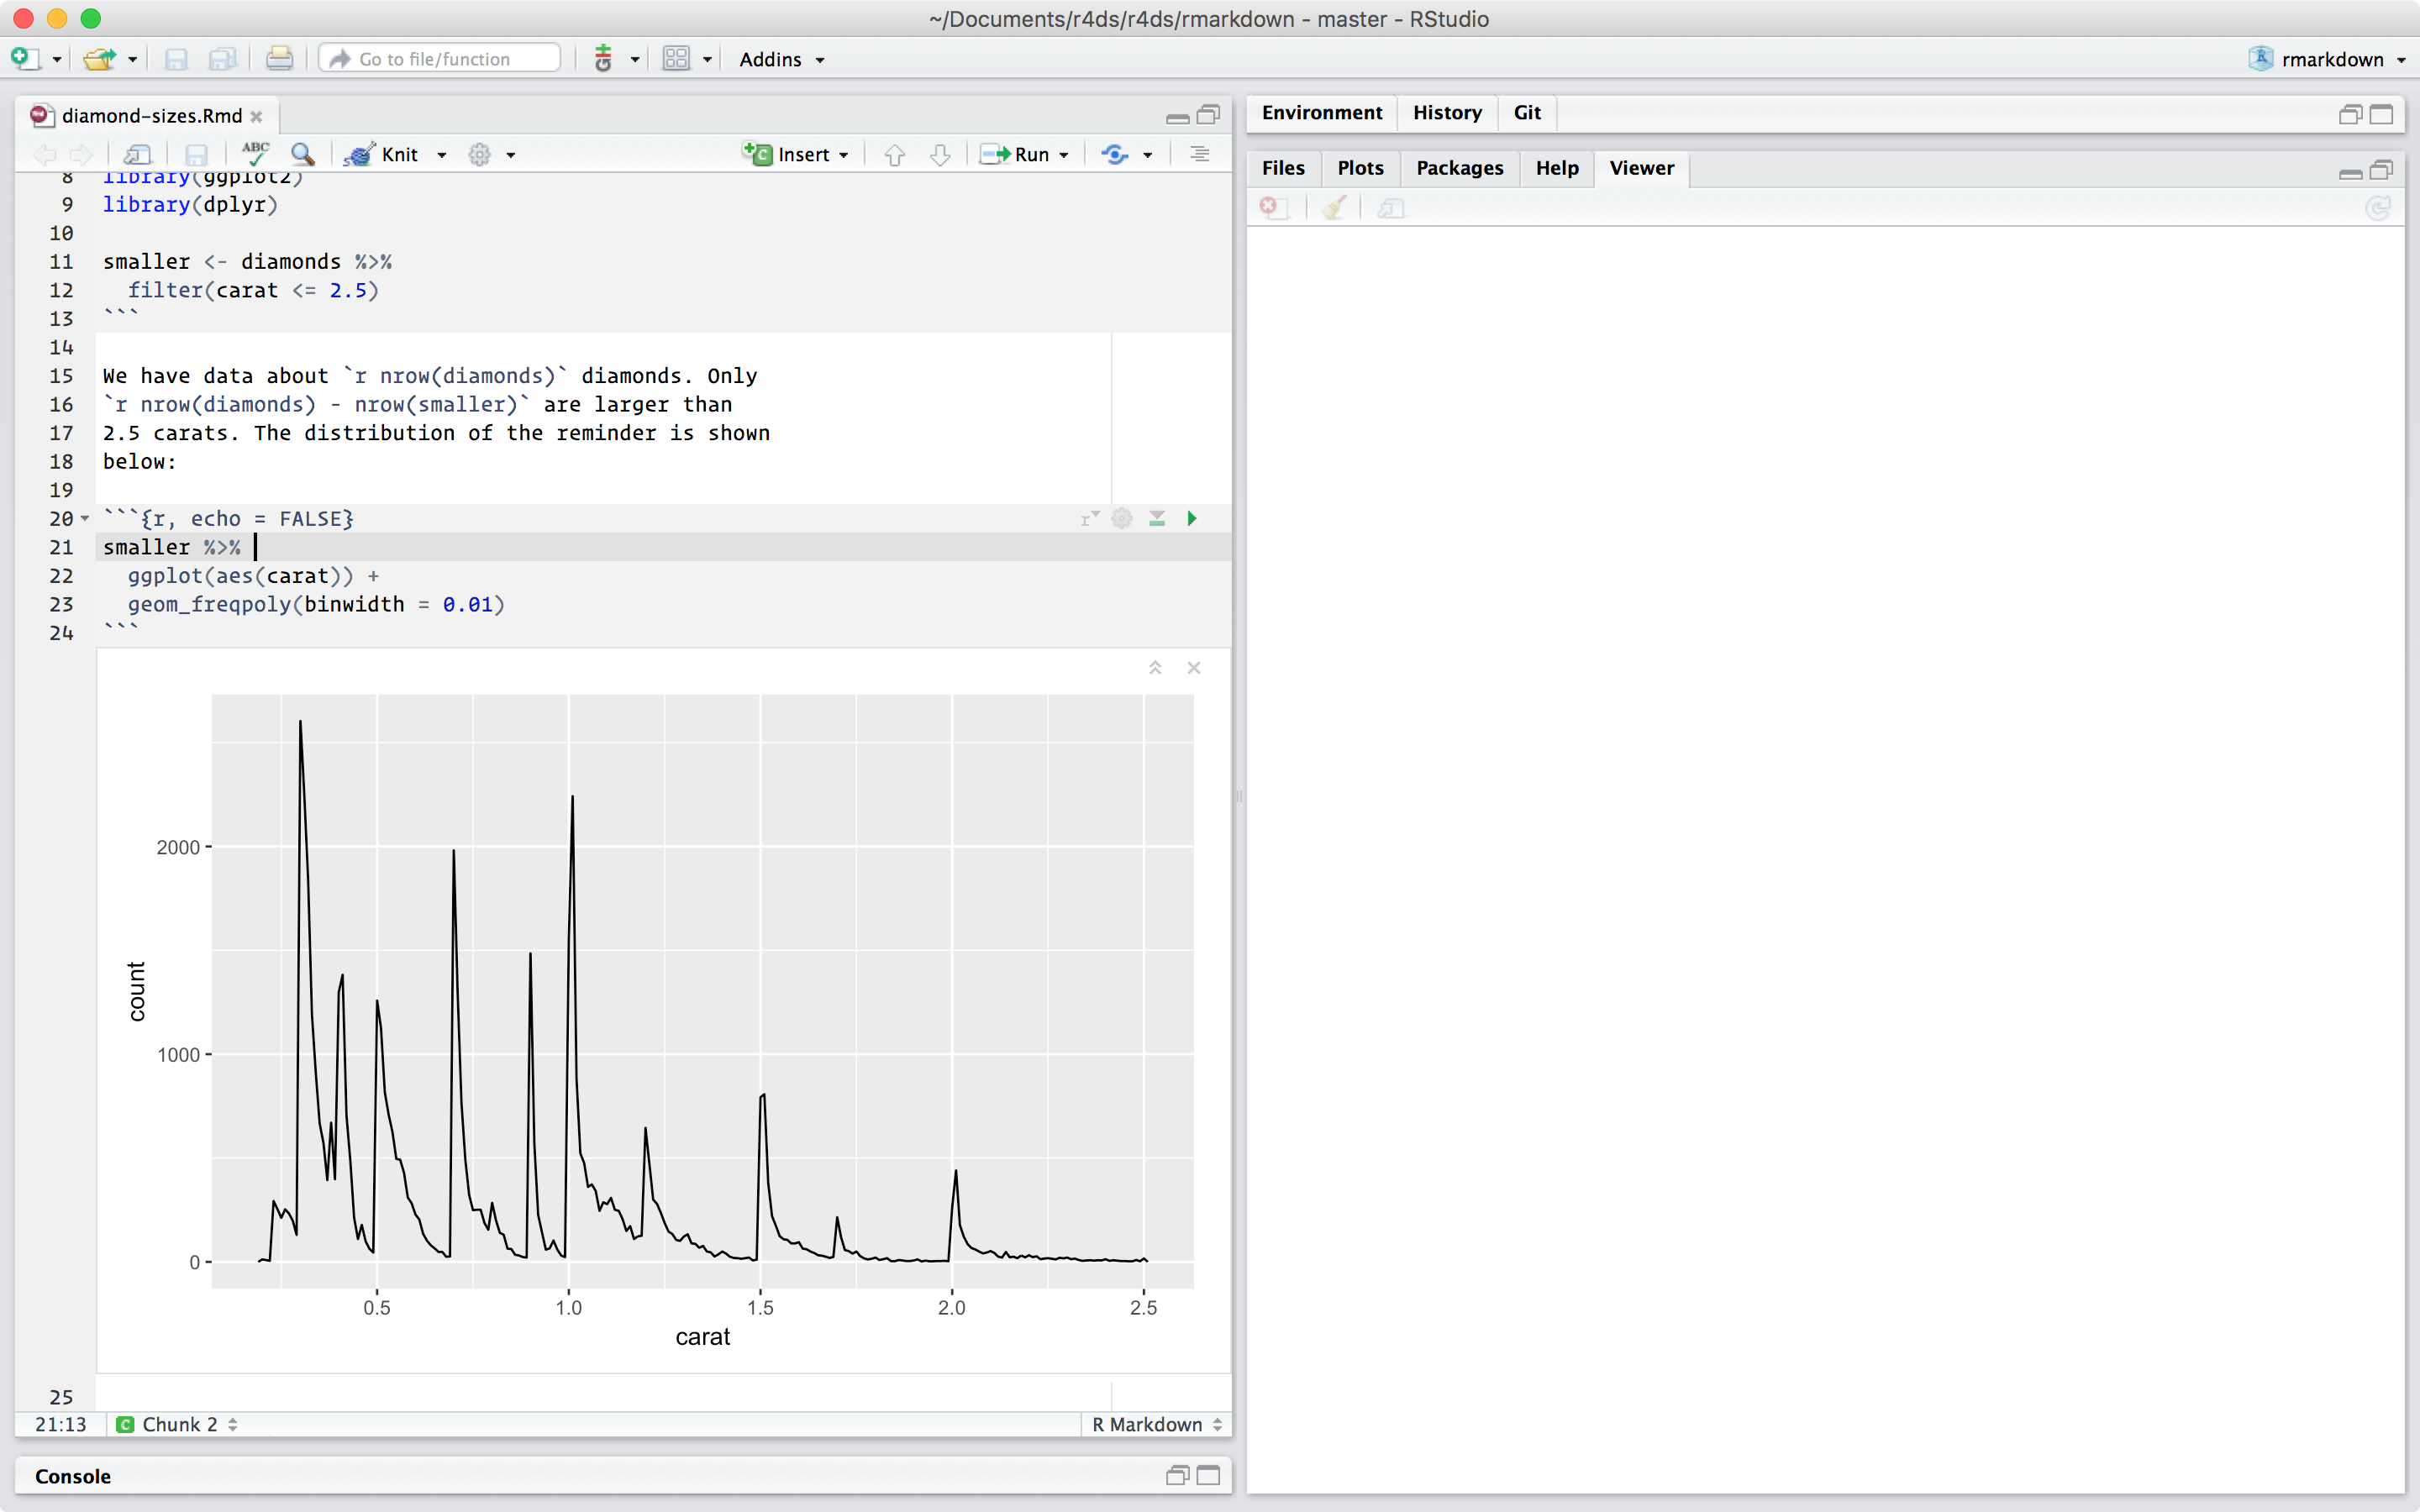
\includegraphics{img/r-markdown.png}
\caption{}
\end{figure}

\subsection{Knitting}\label{knitting}

To produce a complete report containing all text, code, and results,
click the ``Knit'' button at the top of the script editor (it looks like
a ball of yarn) or press \texttt{Cmd/Ctrl\ +\ Shift\ +\ K}. This will
display the report in the viewer pane and create a self-contained HTML
file that you can share with others. The \texttt{.html} file is written
in the same directory as your \texttt{.Rmd} file.

Knitting can be a finicky process that is sometimes challenging to
troubleshoot. You will inevitably run into Knitting errors where RStudio
will tell you that it is unable to knit your \texttt{.Rmd} file. When
this happens, here are some approaches you can try out for
troubleshooting:

\begin{enumerate}
\def\labelenumi{\arabic{enumi}.}
\tightlist
\item
  \textbf{Read the error that RStudio gives you.} Usually, it will tell
  you which line in the code produced the error that stopped the
  Knitting process. Check out this line and see if there is a syntax
  error that needs to be fixed.
\item
  \textbf{Run every code chunk in order, one chunk at a time.} It is
  possible something will not run, which would cause the Knitting error.
  You can also try clearing your environment (in the top right pane)
  before running all the chunks.
\item
  \textbf{Have you copied and pasted text in from other sources?}
  Occasionally, an abnormal character copied from another app can cause
  a Knitting error.
\item
  \textbf{Check all of the file paths} and make sure they are accurate.
\end{enumerate}

This list is by no means exhaustive. The most important step is step 1:
read the error message. You can also try pasting it into Google to see
how other R users have dealt with similar errors.

\subsection{R Chunk Options for
Knitting}\label{r-chunk-options-for-knitting}

You will notice that each R Chunk begins with \texttt{\{r\}}. Within
these brackets, you can add ``Chunk Options'' to the R Chunk that will
dictate how the R Chunk is treated when you Knit the \texttt{.Rmd}. Some
commonly used options are:

\begin{itemize}
\tightlist
\item
  \texttt{eval} (default: \texttt{TRUE}): If \texttt{FALSE}, knitr will
  not run the code in the code chunk (it will, however, still display
  the code in the knitted document).
\item
  \texttt{include} (default: \texttt{TRUE}): If \texttt{FALSE}, knitr
  will run the chunk but hide the code and its results in the final
  document.
\item
  \texttt{echo} (default: \texttt{TRUE}): If \texttt{FALSE}, knitr will
  run the chunk and display the results but hide the code above its
  results in the final document.
\item
  \texttt{error} (default: \texttt{TRUE}): If \texttt{FALSE}, knitr will
  not display any error messages generated by the code.
\item
  \texttt{message} (default: \texttt{TRUE}): If \texttt{FALSE}, knitr
  will not display any messages generated by the code.
\item
  \texttt{warning} (default: \texttt{TRUE}): If \texttt{FALSE}, knitr
  will not display any warnings generated by the code.
\end{itemize}

\subsection{Cheatsheets and Other
Resources}\label{cheatsheets-and-other-resources}

When working in RStudio, you can find an R Markdown cheatsheet by going
to Help \textgreater{} Cheatsheets \textgreater{} R Markdown Cheat
Sheet.

A helpful overview of R Markdown can also be found in
\href{https://r4ds.had.co.nz/r-markdown.html}{R for Data Science}.

A deep dive into R Markdown can be found
\href{https://bookdown.org/yihui/rmarkdown/}{here}.

\subsection{Challenges}\label{challenges}

\subsubsection*{Challenge 1.}\label{challenge-1.}
\addcontentsline{toc}{subsubsection}{Challenge 1.}

Create a new R Markdown document with \emph{File \textgreater{} New File
\textgreater{} R Markdown\ldots{}} Read the instructions. Practice
running the chunks.

Now add some new markdown. Try adding some first-, second-, and
third-level headers. Insert a link to a website.

\subsubsection*{Challenge 2.}\label{challenge-2.}
\addcontentsline{toc}{subsubsection}{Challenge 2.}

In the first code chunk, modify \texttt{cars} to \texttt{mtcars}. Re-run
the chunk and see modified output.

\subsubsection*{Challenge 3.}\label{challenge-3.}
\addcontentsline{toc}{subsubsection}{Challenge 3.}

Knit the document into a PDF file. Verify that you can modify the input
and see the output update.

\subsubsection*{Acknowledgments}\label{acknowledgments-1}
\addcontentsline{toc}{subsubsection}{Acknowledgments}

This page is in part derived from the following sources:

\begin{enumerate}
\def\labelenumi{\arabic{enumi}.}
\item
  \href{https://r4ds.had.co.nz}{R for Data Science}, licensed under
  \href{https://creativecommons.org/licenses/by-nc-nd/3.0/us/}{Creative
  Commons Attribution-NonCommercial-NoDerivs 3.0}.
\item
  \href{https://adv-r.hadley.nz/}{Advanced R}, licensed under
  \href{https://creativecommons.org/licenses/by-nc-sa/4.0/}{Creative
  Commons Attribution-NonCommercial-ShareAlike 4.0 International Public
  License}.
\item
  \href{https://support.rstudio.com/hc/en-us/articles/200484448}{R
  Studio Support}.
\item
  \href{https://moderndive.netlify.com/1-getting-started.html}{A
  ModernDive into R and the tidyverse}.
\end{enumerate}

\chapter{R Syntax}\label{r-syntax}

Frustration is natural when you start programming in R. R is a stickler
for punctuation, and even one character out of place will cause it to
complain. But while you should expect to be a little frustrated, take
comfort in that it is both typical and temporary: it happens to
everyone, and the only way to get over it is to keep trying.

\begin{quote}
To understand computations in R, two slogans are helpful:
\end{quote}

\begin{quote}
\begin{itemize}
\tightlist
\item
  Everything that exists is an object.
\end{itemize}
\end{quote}

\begin{quote}
\begin{itemize}
\tightlist
\item
  Everything that happens is a function call.
\end{itemize}
\end{quote}

\begin{quote}
\textbf{John Chambers}
\end{quote}

\section{Variables}\label{variables}

\subsection{Arithmetic operators}\label{arithmetic-operators}

In its most basic form, R can be used as a simple calculator. Consider
the following arithmetic operators:

\begin{longtable}[]{@{}ll@{}}
\toprule
Operator & Description\tabularnewline
\midrule
\endhead
+ & addition\tabularnewline
- & subtraction\tabularnewline
* & multiplication\tabularnewline
/ & division\tabularnewline
\^{} or ** & exponentiation\tabularnewline
x \%\% y & modulus (remainder)\tabularnewline
\bottomrule
\end{longtable}

\begin{Shaded}
\begin{Highlighting}[]
\DecValTok{1} \OperatorTok{/}\StringTok{ }\DecValTok{200} \OperatorTok{*}\StringTok{ }\DecValTok{30}
\CommentTok{#> [1] 0.15}
\NormalTok{(}\DecValTok{59} \OperatorTok{+}\StringTok{ }\DecValTok{73} \OperatorTok{+}\StringTok{ }\DecValTok{2}\NormalTok{) }\OperatorTok{/}\StringTok{ }\DecValTok{3}
\CommentTok{#> [1] 44.7}
\DecValTok{5} \OperatorTok\StringTok{ }\DecValTok{2}
\CommentTok{#> [1] 1}
\end{Highlighting}
\end{Shaded}

But when we do this, none of our results are saved for later use.

\subsection{Assigning Variables}\label{assigning-variables}

An essential part of programming is creating objects (or
variables).\footnote{Technically, objects and variables are different
  things, but we will use the two interchangeably for now.} Variables
are names for values.

A variable is created when a value is assigned to it. We do that with
\texttt{\textless{}-}.

\begin{Shaded}
\begin{Highlighting}[]
\NormalTok{x <-}\StringTok{ }\DecValTok{3}
\end{Highlighting}
\end{Shaded}

\texttt{\textless{}-} is called the \emph{assignment operator}. It
assigns values on the right to objects on the left, like this:

\begin{Shaded}
\begin{Highlighting}[]
\NormalTok{object_name <-}\StringTok{ }\NormalTok{value}
\end{Highlighting}
\end{Shaded}

So, after executing \texttt{x\ \textless{}-\ 3}, the value of \texttt{x}
is \texttt{3}. The arrow can be read as 3 goes into \texttt{x}.

\textbf{NB}: Do not use \texttt{=} for assignments. It will work in some
contexts, but it will cause confusion later. There will be other
scenarios where you will use \texttt{=} - we will discuss these later
on.

We can use variables in calculations just as if they were values.

\begin{Shaded}
\begin{Highlighting}[]
\NormalTok{x <-}\StringTok{ }\DecValTok{3}
\NormalTok{x }\OperatorTok{+}\StringTok{ }\DecValTok{5}
\CommentTok{#> [1] 8}
\end{Highlighting}
\end{Shaded}

\subsubsection*{Inspect objects to display
values.}\label{inspect-objects-to-display-values.}
\addcontentsline{toc}{subsubsection}{Inspect objects to display values.}

In R, the contents of an object can be printed by simply executing the
object name.

\begin{Shaded}
\begin{Highlighting}[]
\NormalTok{x <-}\StringTok{ }\DecValTok{3}
\NormalTok{x}
\CommentTok{#> [1] 3}
\end{Highlighting}
\end{Shaded}

\subsubsection*{Whitespace makes code easier to
read.}\label{whitespace-makes-code-easier-to-read.}
\addcontentsline{toc}{subsubsection}{Whitespace makes code easier to
read.}

Notice that we surrounded \texttt{\textless{}-} with spaces. In R, white
space is ignored (unlike Python). It is good practice to use spaces,
because it makes code easier to read.

\begin{Shaded}
\begin{Highlighting}[]
\NormalTok{experiment<-}\StringTok{"current vs. voltage"}   \CommentTok{# this is bad}
\NormalTok{experiment <-}\StringTok{ "current vs. voltage"} \CommentTok{# this is better}
\end{Highlighting}
\end{Shaded}

\subsection{Variable Names}\label{variable-names}

Object names can only contain letters, numbers, \texttt{\_} and
\texttt{.}.

You want your object names to be descriptive. \texttt{x} is not a good
variable name (sorry!). You will also need a convention for multiple
words. I recommend \emph{snake\_case}, where you separate lowercase
words with \texttt{\_}.

\begin{Shaded}
\begin{Highlighting}[]
\NormalTok{i_use_snake_case}
\NormalTok{otherPeopleUseCamelCase}
\NormalTok{some.people.use.periods}
\NormalTok{And_aFew.People_RENOUNCEconvention}
\end{Highlighting}
\end{Shaded}

Let's make an assignment using snake\_case:

\begin{Shaded}
\begin{Highlighting}[]
\NormalTok{r_rocks <-}\StringTok{ }\DecValTok{2} \OperatorTok{^}\StringTok{ }\DecValTok{3}
\end{Highlighting}
\end{Shaded}

And let's try to inspect it:

\begin{Shaded}
\begin{Highlighting}[]
\NormalTok{r_rock}
\CommentTok{#> Error in eval(expr, envir, enclos): object 'r_rock' not found}
\NormalTok{R_rocks}
\CommentTok{#> Error in eval(expr, envir, enclos): object 'R_rocks' not found}
\end{Highlighting}
\end{Shaded}

R is case-sensitive!

\subsubsection*{Use the TAB key to
autocomplete.}\label{use-the-tab-key-to-autocomplete.}
\addcontentsline{toc}{subsubsection}{Use the TAB key to autocomplete.}

Because typos are the absolute worst, we can use R Studio to help us
type. Let's inspect \texttt{r\_rocks} using RStudio's tab completion
facility. Type \texttt{r\_}, press TAB, add characters until you have a
unique prefix, then press return.

\begin{Shaded}
\begin{Highlighting}[]
\NormalTok{r_rocks}
\CommentTok{#> [1] 8}
\end{Highlighting}
\end{Shaded}

\subsection{Challenges}\label{challenges-1}

\subsubsection*{Challenge 1: Making and printing
variables.}\label{challenge-1-making-and-printing-variables.}
\addcontentsline{toc}{subsubsection}{Challenge 1: Making and printing
variables.}

Make 3 variables: name (with your full name), city (where you were
born), and year (when you were born).

\subsubsection*{Challenge 2: Swapping
values.}\label{challenge-2-swapping-values.}
\addcontentsline{toc}{subsubsection}{Challenge 2: Swapping values.}

Draw a table showing the values of the variables in this program after
each statement is executed.

In simple terms, what do the last three lines of this program do?

\begin{Shaded}
\begin{Highlighting}[]
\NormalTok{lowest <-}\StringTok{ }\FloatTok{1.0}
\NormalTok{highest <-}\StringTok{ }\FloatTok{3.0}
\NormalTok{temp <-}\StringTok{ }\NormalTok{lowest}
\NormalTok{lowest <-}\StringTok{ }\NormalTok{highest}
\NormalTok{highest <-}\StringTok{ }\NormalTok{temp}
\end{Highlighting}
\end{Shaded}

\subsubsection*{Challenge 3: Predicting
values.}\label{challenge-3-predicting-values.}
\addcontentsline{toc}{subsubsection}{Challenge 3: Predicting values.}

What is the final value of \texttt{position} in the program below? Try
to predict the value without running the program, then check your
prediction.

\begin{Shaded}
\begin{Highlighting}[]
\NormalTok{initial <-}\StringTok{ "left"}
\NormalTok{position <-}\StringTok{ }\NormalTok{initial}
\NormalTok{initial <-}\StringTok{ "right"}
\end{Highlighting}
\end{Shaded}

\subsubsection*{Challenge 4: Syntax.}\label{challenge-4-syntax.}
\addcontentsline{toc}{subsubsection}{Challenge 4: Syntax.}

Why does the following code fail?

\begin{Shaded}
\begin{Highlighting}[]
\NormalTok{age }\OperatorTok{==}\StringTok{ }\DecValTok{31}
\end{Highlighting}
\end{Shaded}

And the following?

\begin{Shaded}
\begin{Highlighting}[]
\DecValTok{31}\NormalTok{ <-}\StringTok{  }\NormalTok{age}
\end{Highlighting}
\end{Shaded}

\section{Functions}\label{functions}

R has a large collection of built-in functions that helps us do things.
When we use a function, we say we are \emph{calling} a function.

\begin{Shaded}
\begin{Highlighting}[]
\KeywordTok{function_name}\NormalTok{(}\DataTypeTok{arg1 =}\NormalTok{ val1, }\DataTypeTok{arg2 =}\NormalTok{ val2, ...)}
\end{Highlighting}
\end{Shaded}

Here are some helpful built-in functions:

\begin{Shaded}
\begin{Highlighting}[]
\NormalTok{my_var <-}\StringTok{ }\KeywordTok{c}\NormalTok{(}\DecValTok{1}\NormalTok{, }\DecValTok{5}\NormalTok{, }\DecValTok{2}\NormalTok{, }\DecValTok{4}\NormalTok{, }\DecValTok{5}\NormalTok{)}

\KeywordTok{sum}\NormalTok{(my_var)}
\CommentTok{#> [1] 17}
\KeywordTok{length}\NormalTok{(my_var)}
\CommentTok{#> [1] 5}
\KeywordTok{min}\NormalTok{(my_var)}
\CommentTok{#> [1] 1}
\KeywordTok{max}\NormalTok{(my_var)}
\CommentTok{#> [1] 5}
\KeywordTok{unique}\NormalTok{(my_var)}
\CommentTok{#> [1] 1 5 2 4}
\end{Highlighting}
\end{Shaded}

\subsection{Arguments}\label{arguments}

An \emph{argument} is a value that is \emph{passed} into a function.
Every function returns a \emph{result}.

Let's try using \texttt{seq()}, which makes regular sequences of
numbers. While we are at it, we will learn more helpful features of
RStudio.

Type \texttt{se} and hit TAB. A popup shows you possible completions.
Specify \texttt{seq()} by typing more (a \texttt{q}) to disambiguate, or
by using ↑/↓ arrows to select. Notice the floating tooltip that pops up,
reminding you of the function's arguments and purpose.

Press TAB once more when you have selected the function you want.
RStudio will add matching opening (\texttt{(}) and closing (\texttt{)})
parentheses for you. Type the arguments \texttt{1,\ 10} and hit return.

\begin{Shaded}
\begin{Highlighting}[]
\KeywordTok{seq}\NormalTok{(}\DecValTok{1}\NormalTok{, }\DecValTok{10}\NormalTok{)}
\CommentTok{#>  [1]  1  2  3  4  5  6  7  8  9 10}
\end{Highlighting}
\end{Shaded}

How many arguments did we pass into the \texttt{seq} function?

\subsection{Store Function Output}\label{store-function-output}

Notice that, when we called the \texttt{seq} function, nothing changed
in our environment. That is because we did not save our results to an
object. Let's try it again by assigning a variable:

\begin{Shaded}
\begin{Highlighting}[]
\NormalTok{y <-}\StringTok{ }\KeywordTok{seq}\NormalTok{(}\DecValTok{1}\NormalTok{, }\DecValTok{10}\NormalTok{)}
\NormalTok{y}
\CommentTok{#>  [1]  1  2  3  4  5  6  7  8  9 10}
\end{Highlighting}
\end{Shaded}

\subsection{Argument Restrictions and
Defaults}\label{argument-restrictions-and-defaults}

Let's use another function, called \texttt{round}:

\begin{Shaded}
\begin{Highlighting}[]
\KeywordTok{round}\NormalTok{(}\FloatTok{60.123}\NormalTok{)}
\CommentTok{#> [1] 60}
\end{Highlighting}
\end{Shaded}

\texttt{round} must be given at least one argument. Moreover, it must be
given things that can be meaningfully rounded.

\begin{Shaded}
\begin{Highlighting}[]
\KeywordTok{round}\NormalTok{()}
\KeywordTok{round}\NormalTok{(}\StringTok{'a'}\NormalTok{)}
\end{Highlighting}
\end{Shaded}

Functions may have \textbf{default} values for some arguments.

By default, \texttt{round} will round off any number to zero decimal
places. But we can specify the number of decimal places we want.

\begin{Shaded}
\begin{Highlighting}[]
\KeywordTok{round}\NormalTok{(}\FloatTok{60.123}\NormalTok{)}
\CommentTok{#> [1] 60}
\KeywordTok{round}\NormalTok{(}\FloatTok{60.123}\NormalTok{, }\DataTypeTok{digits =} \DecValTok{2}\NormalTok{)}
\CommentTok{#> [1] 60.1}
\KeywordTok{round}\NormalTok{(}\FloatTok{60.123}\NormalTok{, }\DecValTok{2}\NormalTok{)}
\CommentTok{#> [1] 60.1}
\end{Highlighting}
\end{Shaded}

\subsection{Documentation and Help
Files}\label{documentation-and-help-files}

How do we know what kinds of arguments to pass into a function? Every
built-in function comes with \textbf{documentation}.

\begin{itemize}
\tightlist
\item
  \texttt{?} + object opens a help page for that specific object.
\item
  \texttt{??} + object searches help pages containing the name of the
  object.
\end{itemize}

\begin{Shaded}
\begin{Highlighting}[]
\NormalTok{?mean}
\NormalTok{??mean}
\end{Highlighting}
\end{Shaded}

All help files are structured the same way:

\begin{itemize}
\tightlist
\item
  The \textbf{Arguments} section tells us exactly what kind of
  information we can pass into a function.
\item
  The \textbf{Value} section explains what the output of the function
  is.
\item
  The \textbf{Examples} section contains real examples of the function
  in use.
\end{itemize}

\subsection{Challenges}\label{challenges-2}

\subsubsection*{Challenge 1: What Happens
When}\label{challenge-1-what-happens-when}
\addcontentsline{toc}{subsubsection}{Challenge 1: What Happens When}

Explain, in simple terms, the order of operations in the following
program: When does the addition happen, when does the subtraction
happen, when is each function called, etc.

What is the final value of \texttt{radiance}?

\begin{Shaded}
\begin{Highlighting}[]
\NormalTok{radiance <-}\StringTok{ }\FloatTok{1.0}
\NormalTok{radiance <-}\StringTok{ }\KeywordTok{max}\NormalTok{(}\FloatTok{2.1}\NormalTok{, }\FloatTok{2.0} \OperatorTok{+}\StringTok{ }\KeywordTok{min}\NormalTok{(radiance, }\FloatTok{1.1} \OperatorTok{*}\StringTok{ }\NormalTok{radiance }\OperatorTok{-}\StringTok{ }\FloatTok{0.5}\NormalTok{))}
\end{Highlighting}
\end{Shaded}

\subsubsection*{Challenge 2: Why?}\label{challenge-2-why}
\addcontentsline{toc}{subsubsection}{Challenge 2: Why?}

Run the following code.

\begin{Shaded}
\begin{Highlighting}[]
\NormalTok{rich <-}\StringTok{ "gold"}
\NormalTok{poor <-}\StringTok{ "tin"}
\KeywordTok{max}\NormalTok{(rich, poor)}
\end{Highlighting}
\end{Shaded}

Using the help files for \texttt{max}, explain why it returns the result
it does.

\section{Data Types}\label{data-types}

Every value in a program has a specific \textbf{type}. In R, those types
are called ``classes'', and there are 4 of them:

\begin{itemize}
\tightlist
\item
  Character (text or ``string'').
\item
  Numeric (integer or decimal).
\item
  Integer (just integer).
\item
  Logical (TRUE or FALSE booleans).
\end{itemize}

\begin{longtable}[]{@{}ll@{}}
\toprule
Example & Type\tabularnewline
\midrule
\endhead
``a'', ``swc'' & character\tabularnewline
2, 15.5 & numeric\tabularnewline
2 (Must add a \texttt{L} at end to denote integer) &
integer\tabularnewline
\texttt{TRUE}, \texttt{FALSE} & logical\tabularnewline
\bottomrule
\end{longtable}

\subsection{What Is that Type?}\label{what-is-that-type}

R is dynamically typed, meaning that it ``guesses'' what class a value
is. Every piece of information in R has a type!

Use the built-in function \texttt{class()} to find out what type a value
has.

\begin{Shaded}
\begin{Highlighting}[]
\KeywordTok{class}\NormalTok{(}\DecValTok{3}\NormalTok{)}
\CommentTok{#> [1] "numeric"}
\KeywordTok{class}\NormalTok{(3L)}
\CommentTok{#> [1] "integer"}
\KeywordTok{class}\NormalTok{(}\StringTok{"Three"}\NormalTok{)}
\CommentTok{#> [1] "character"}
\KeywordTok{class}\NormalTok{(T)}
\CommentTok{#> [1] "logical"}
\end{Highlighting}
\end{Shaded}

This works on variables as well. But remember: the \emph{value} has the
type --- the \emph{variable} is just a label.

\begin{Shaded}
\begin{Highlighting}[]
\NormalTok{three <-}\StringTok{ }\DecValTok{3}
\KeywordTok{class}\NormalTok{(three)}
\CommentTok{#> [1] "numeric"}

\NormalTok{three <-}\StringTok{ "three"}
\KeywordTok{class}\NormalTok{(three)}
\CommentTok{#> [1] "character"}
\end{Highlighting}
\end{Shaded}

A value's class determines what the program can do to it.

\begin{Shaded}
\begin{Highlighting}[]
\DecValTok{3} \OperatorTok{-}\StringTok{ }\DecValTok{1}
\CommentTok{#> [1] 2}
\DecValTok{3} \OperatorTok{-}\StringTok{ "1"}
\CommentTok{#> Error in 3 - "1": non-numeric argument to binary operator}
\end{Highlighting}
\end{Shaded}

\subsection{Coercion}\label{coercion}

We just learned we cannot subtract numbers and strings. Instead, use
\texttt{as.} + name of class as a function to convert a value to a
specified type.

\begin{Shaded}
\begin{Highlighting}[]
\DecValTok{3} \OperatorTok{-}\StringTok{ }\KeywordTok{as.numeric}\NormalTok{(}\StringTok{"1"}\NormalTok{)}
\end{Highlighting}
\end{Shaded}

This is called \texttt{coercion}. Here is another example:

\begin{Shaded}
\begin{Highlighting}[]
\NormalTok{my_var <-}\StringTok{ "FALSE"}
\NormalTok{my_var}
\CommentTok{#> [1] "FALSE"}
\KeywordTok{as.logical}\NormalTok{(my_var)}
\CommentTok{#> [1] FALSE}
\end{Highlighting}
\end{Shaded}

What difference did you notice?

\subsection{Other Objects}\label{other-objects}

There are a few other ``odd ball'' types in R:

\subsubsection*{\texorpdfstring{\texttt{NA} are missing
values.}{NA are missing values.}}\label{na-are-missing-values.}
\addcontentsline{toc}{subsubsection}{\texttt{NA} are missing values.}

Missing values are specified with \texttt{NA}. \texttt{NA} will always
be coerced to the correct type if used inside \texttt{c()}.

\begin{Shaded}
\begin{Highlighting}[]
\NormalTok{x <-}\StringTok{ }\KeywordTok{c}\NormalTok{(}\OtherTok{NA}\NormalTok{, }\DecValTok{1}\NormalTok{)}
\NormalTok{x}
\CommentTok{#> [1] NA  1}
\KeywordTok{typeof}\NormalTok{(}\OtherTok{NA}\NormalTok{)}
\CommentTok{#> [1] "logical"}
\KeywordTok{typeof}\NormalTok{(x)}
\CommentTok{#> [1] "double"}
\end{Highlighting}
\end{Shaded}

\subsubsection*{\texorpdfstring{\texttt{Inf} is
infinity.}{Inf is infinity.}}\label{inf-is-infinity.}
\addcontentsline{toc}{subsubsection}{\texttt{Inf} is infinity.}

You can have either positive or negative infinity.

\begin{Shaded}
\begin{Highlighting}[]
\DecValTok{1}\OperatorTok{/}\DecValTok{0}
\CommentTok{#> [1] Inf}
\DecValTok{1}\OperatorTok{/}\OtherTok{Inf}
\CommentTok{#> [1] 0}
\end{Highlighting}
\end{Shaded}

\subsubsection*{\texorpdfstring{\texttt{NaN} means ``not a number.'' It
is an undefined
value.}{NaN means not a number. It is an undefined value.}}\label{nan-means-not-a-number.-it-is-an-undefined-value.}
\addcontentsline{toc}{subsubsection}{\texttt{NaN} means ``not a
number.'' It is an undefined value.}

\begin{Shaded}
\begin{Highlighting}[]
\DecValTok{0}\OperatorTok{/}\DecValTok{0}
\CommentTok{#> [1] NaN}
\end{Highlighting}
\end{Shaded}

\subsection{Challenges}\label{challenges-3}

\subsubsection*{Challenge 1: Making and Coercing
Variables}\label{challenge-1-making-and-coercing-variables}
\addcontentsline{toc}{subsubsection}{Challenge 1: Making and Coercing
Variables}

\begin{enumerate}
\def\labelenumi{\arabic{enumi}.}
\tightlist
\item
  Make a variable \texttt{year} and assign it as the year you were born.
\item
  Coerce that variable to a string and assign it to a new variable
  \texttt{year\_string}.
\item
  Someone in your class says they were born in 2001. Really? Really.
  Find out what your age difference is, using only
  \texttt{year\_string}.
\end{enumerate}

\subsubsection*{Challenge 2: Fixing the
Code}\label{challenge-2-fixing-the-code}
\addcontentsline{toc}{subsubsection}{Challenge 2: Fixing the Code}

Change the following code to make the output \texttt{TRUE}:

\begin{Shaded}
\begin{Highlighting}[]
\NormalTok{val_}\DecValTok{1}\NormalTok{ <-}\StringTok{ }\NormalTok{F}
\NormalTok{val_}\DecValTok{2}\NormalTok{ <-}\StringTok{ "F"}

\KeywordTok{class}\NormalTok{(val_}\DecValTok{1}\NormalTok{) }\OperatorTok{==}\StringTok{ }\KeywordTok{class}\NormalTok{(val_}\DecValTok{2}\NormalTok{)}
\CommentTok{#> [1] FALSE}
\end{Highlighting}
\end{Shaded}

\section{Boolean Expressions}\label{boolean-expressions}

Boolean expressions are logical statements that are either true or
false. For our purposes, we will often use Boolean expressions to
compare quantities. For instance, the Boolean expression
\texttt{1\ \textless{}\ 2} is true, whereas the Boolean expression
\texttt{1\ \textgreater{}\ 2} is false.

When you type a Boolean expression in R, R will output \texttt{TRUE} if
the expression is true and \texttt{FALSE} if the expression is false.

\subsection{Boolean Operators}\label{boolean-operators}

\begin{longtable}[]{@{}ll@{}}
\toprule
Operator & Description\tabularnewline
\midrule
\endhead
\texttt{\textless{}} & less than\tabularnewline
\texttt{\textless{}=} & less than or equal to\tabularnewline
\texttt{\textgreater{}} & greater than\tabularnewline
\texttt{\textgreater{}=} & greater than or equal to\tabularnewline
\texttt{==} & exactly equal to\tabularnewline
\texttt{!=} & not equal to\tabularnewline
\texttt{\%in\%} & is an item of a set\tabularnewline
\bottomrule
\end{longtable}

Note that we use a double equal sign \texttt{==} to check whether two
values are equal. Typing \texttt{a\ =\ b} would set the value of
\texttt{a} equal to the value of \texttt{b}.

Here are some examples of Boolean expressions in action:

\begin{Shaded}
\begin{Highlighting}[]
\DecValTok{1} \OperatorTok{<}\StringTok{ }\DecValTok{2}
\CommentTok{#> [1] TRUE}
\DecValTok{1} \OperatorTok{>}\StringTok{ }\DecValTok{2}
\CommentTok{#> [1] FALSE}
\DecValTok{1} \OperatorTok{==}\StringTok{ }\DecValTok{2}
\CommentTok{#> [1] FALSE}

\NormalTok{value_}\DecValTok{1}\NormalTok{ <-}\StringTok{ }\DecValTok{1}
\NormalTok{value_}\DecValTok{1} \OperatorTok{>}\StringTok{ }\DecValTok{0}
\CommentTok{#> [1] TRUE}

\NormalTok{value_}\DecValTok{2}\NormalTok{ <-}\StringTok{ }\NormalTok{value_}\DecValTok{1} \OperatorTok{+}\StringTok{ }\DecValTok{10}
\NormalTok{value_}\DecValTok{1} \OperatorTok{+}\StringTok{ }\NormalTok{value_}\DecValTok{2} \OperatorTok{<=}\StringTok{ }\DecValTok{12}
\CommentTok{#> [1] TRUE}
\end{Highlighting}
\end{Shaded}

\subsection{Logical Operators}\label{logical-operators}

In practice, we often use two or more conditions to decide what to do.
To combine different conditions, there are three logical operators:

\begin{longtable}[]{@{}ll@{}}
\toprule
Operator & Description\tabularnewline
\midrule
\endhead
\texttt{x\ \&\ y} & \texttt{x} AND y\tabularnewline
\texttt{x\ \textbar{}\ y} & \texttt{x} OR y\tabularnewline
\texttt{!x} & Not \texttt{x}\tabularnewline
\bottomrule
\end{longtable}

First, \texttt{\&} is similar to \textbf{AND} in English, that is,
\texttt{x\ \&\ y} is true only if both \texttt{x} and \texttt{y} are
true. Second, is similar to \textbf{OR} in English, that is, A
\textbar{}\textbar{} B is false only if both \texttt{x} and \texttt{y}
are false. Third, \texttt{!} is similar to \textbf{NOT} in English, that
is, \texttt{!x} is true only if \texttt{x} is false.

\begin{Shaded}
\begin{Highlighting}[]
\NormalTok{x <-}\StringTok{ }\DecValTok{10}
\NormalTok{y <-}\StringTok{ }\DecValTok{20}

\CommentTok{# check to see if values are between 5 and 15}
\NormalTok{x }\OperatorTok{>}\StringTok{ }\DecValTok{5} \OperatorTok{&}\StringTok{ }\NormalTok{x }\OperatorTok{<}\StringTok{ }\DecValTok{15}
\CommentTok{#> [1] TRUE}
\NormalTok{y }\OperatorTok{>}\StringTok{ }\DecValTok{5} \OperatorTok{&}\StringTok{ }\NormalTok{y }\OperatorTok{<}\StringTok{ }\DecValTok{15}
\CommentTok{#> [1] FALSE}

\CommentTok{# more complex chains}
\NormalTok{(x }\OperatorTok{>}\StringTok{ }\DecValTok{5} \OperatorTok{&}\StringTok{ }\NormalTok{x }\OperatorTok{<}\StringTok{ }\DecValTok{15}\NormalTok{) }\OperatorTok{&}\StringTok{ }\NormalTok{(x }\OperatorTok{>}\StringTok{ }\NormalTok{y }\OperatorTok{&}\StringTok{ }\NormalTok{y }\OperatorTok{<}\StringTok{ }\DecValTok{15}\NormalTok{)}
\CommentTok{#> [1] FALSE}
\NormalTok{(x }\OperatorTok{>}\StringTok{ }\DecValTok{5} \OperatorTok{&}\StringTok{ }\NormalTok{x }\OperatorTok{<}\StringTok{ }\DecValTok{15}\NormalTok{) }\OperatorTok{|}\StringTok{ }\NormalTok{(x }\OperatorTok{>}\StringTok{ }\NormalTok{y }\OperatorTok{&}\StringTok{ }\NormalTok{y }\OperatorTok{<}\StringTok{ }\DecValTok{15}\NormalTok{)}
\CommentTok{#> [1] TRUE}
\NormalTok{(x }\OperatorTok{>}\StringTok{ }\DecValTok{5} \OperatorTok{&}\StringTok{ }\NormalTok{x }\OperatorTok{<}\StringTok{ }\DecValTok{15}\NormalTok{) }\OperatorTok{&}\StringTok{ }\OperatorTok{!}\NormalTok{(x }\OperatorTok{>}\StringTok{ }\NormalTok{y }\OperatorTok{&}\StringTok{ }\NormalTok{y }\OperatorTok{<}\StringTok{ }\DecValTok{15}\NormalTok{)}
\CommentTok{#> [1] TRUE}
\end{Highlighting}
\end{Shaded}

Different operator take different precendence. It is always a good
practice to use brackets to control operation ordering.

\subsection{Boolean Vectors}\label{boolean-vectors}

The nice thing about R is that you can use these comparison operators
also on vectors. As with many expressions in R, the Boolean expressions
discussed above are all \emph{vectorized.} We will learn more about
vectors and vectorization later in this class, but here is a quick
example:

\begin{Shaded}
\begin{Highlighting}[]
\NormalTok{x <-}\StringTok{ }\KeywordTok{c}\NormalTok{(}\FloatTok{2.1}\NormalTok{, }\FloatTok{4.2}\NormalTok{, }\FloatTok{3.3}\NormalTok{, }\FloatTok{5.4}\NormalTok{)}
\NormalTok{x }\OperatorTok{>}\StringTok{ }\DecValTok{3}
\CommentTok{#> [1] FALSE  TRUE  TRUE  TRUE}
\end{Highlighting}
\end{Shaded}

This command tests for every element of the vector if the condition
stated by the comparison operator is \texttt{TRUE} or \texttt{FALSE}.

\subsection{Boolean Vectors in Action}\label{boolean-vectors-in-action}

Boolean vectors are partially what makes R so magical. Check out the
example below and examine each line. We will cover subsetting operations
later, but pay attention to the work of boolean expressions and logical
operators.

\begin{Shaded}
\begin{Highlighting}[]
\CommentTok{# An example}
\NormalTok{x <-}\StringTok{ }\KeywordTok{c}\NormalTok{(}\DecValTok{1}\OperatorTok{:}\DecValTok{10}\NormalTok{)}
\NormalTok{x[(x}\OperatorTok{>}\DecValTok{8}\NormalTok{) }\OperatorTok{|}\StringTok{ }\NormalTok{(x}\OperatorTok{<}\DecValTok{5}\NormalTok{)]}
\CommentTok{#> [1]  1  2  3  4  9 10}

\CommentTok{# How it works}
\NormalTok{x <-}\StringTok{ }\KeywordTok{c}\NormalTok{(}\DecValTok{1}\OperatorTok{:}\DecValTok{10}\NormalTok{)}
\NormalTok{x}
\CommentTok{#>  [1]  1  2  3  4  5  6  7  8  9 10}
\NormalTok{x }\OperatorTok{>}\StringTok{ }\DecValTok{8}
\CommentTok{#>  [1] FALSE FALSE FALSE FALSE FALSE FALSE FALSE FALSE  TRUE  TRUE}
\NormalTok{x }\OperatorTok{<}\StringTok{ }\DecValTok{5}
\CommentTok{#>  [1]  TRUE  TRUE  TRUE  TRUE FALSE FALSE FALSE FALSE FALSE FALSE}
\NormalTok{x }\OperatorTok{>}\StringTok{ }\DecValTok{8} \OperatorTok{|}\StringTok{ }\NormalTok{x }\OperatorTok{<}\StringTok{ }\DecValTok{5}
\CommentTok{#>  [1]  TRUE  TRUE  TRUE  TRUE FALSE FALSE FALSE FALSE  TRUE  TRUE}
\NormalTok{x[}\KeywordTok{c}\NormalTok{(T,T,T,T,F,F,F,F,T,T)]}
\CommentTok{#> [1]  1  2  3  4  9 10}
\end{Highlighting}
\end{Shaded}

\subsection{Challenges}\label{challenges-4}

\subsubsection*{Challenge 1.}\label{challenge-1.-1}
\addcontentsline{toc}{subsubsection}{Challenge 1.}

In the partially written code below, \texttt{vector\_1} and
\texttt{vector\_2} each contain 10 values. Using the fact that Boolean
expressions are vectorized, write code that outputs:

\begin{enumerate}
\def\labelenumi{\arabic{enumi}.}
\tightlist
\item
  A vector of length 10 such that element \texttt{i} of this vector
  equals \texttt{TRUE} if \texttt{vector\_1{[}i{]}} is less than
  \texttt{vector\_2{[}i{]}} and equals \texttt{FALSE} otherwise.
\item
  The number of times that element \texttt{i} of \texttt{vector\_1} is
  less than element \texttt{i} of \texttt{vector\_2}, using the
  \texttt{sum} function.
\end{enumerate}

\begin{Shaded}
\begin{Highlighting}[]
\NormalTok{vector_}\DecValTok{1}\NormalTok{ <-}\StringTok{ }\KeywordTok{c}\NormalTok{(}\DecValTok{1}\NormalTok{, }\DecValTok{2}\NormalTok{, }\DecValTok{4}\NormalTok{, }\DecValTok{5}\NormalTok{, }\DecValTok{3}\NormalTok{, }\DecValTok{7}\NormalTok{, }\DecValTok{8}\NormalTok{, }\DecValTok{7}\NormalTok{, }\DecValTok{1}\NormalTok{, }\DecValTok{2}\NormalTok{)}
\NormalTok{vector_}\DecValTok{2}\NormalTok{ <-}\StringTok{ }\KeywordTok{c}\NormalTok{(}\DecValTok{1}\NormalTok{, }\DecValTok{3}\NormalTok{, }\DecValTok{4}\NormalTok{, }\DecValTok{4}\NormalTok{, }\DecValTok{5}\NormalTok{, }\DecValTok{10}\NormalTok{, }\DecValTok{6}\NormalTok{, }\DecValTok{8}\NormalTok{, }\DecValTok{9}\NormalTok{, }\DecValTok{1}\NormalTok{)}

\CommentTok{# YOUR CODE HERE}
\end{Highlighting}
\end{Shaded}

\chapter{Working with Data}\label{working-with-data}

This unit will cover the basics of working with data, including project
workflow, data terms and concepts, importing data, and exploring data.

\section{Project Workflow}\label{project-workflow}

One day\ldots{}

\begin{itemize}
\tightlist
\item
  You will need to quit R, go do something else, and return to your
  analysis the next day.
\item
  You will be working on multiple projects simultaneously, and you will
  want to keep them separate.
\item
  You will need to bring data from the outside world into R and send
  numerical results and figures from R back out into the world.
\end{itemize}

This unit will teach you how to set up your workflow to make the best
use of R.

\subsection{Store Analyses in Scripts, Not
Workspaces}\label{store-analyses-in-scripts-not-workspaces}

R Studio automatically preserves your workspace (environment and command
history) when you quit R and re-loads it the next session. I recommend
you turn this behavior off.

\begin{center}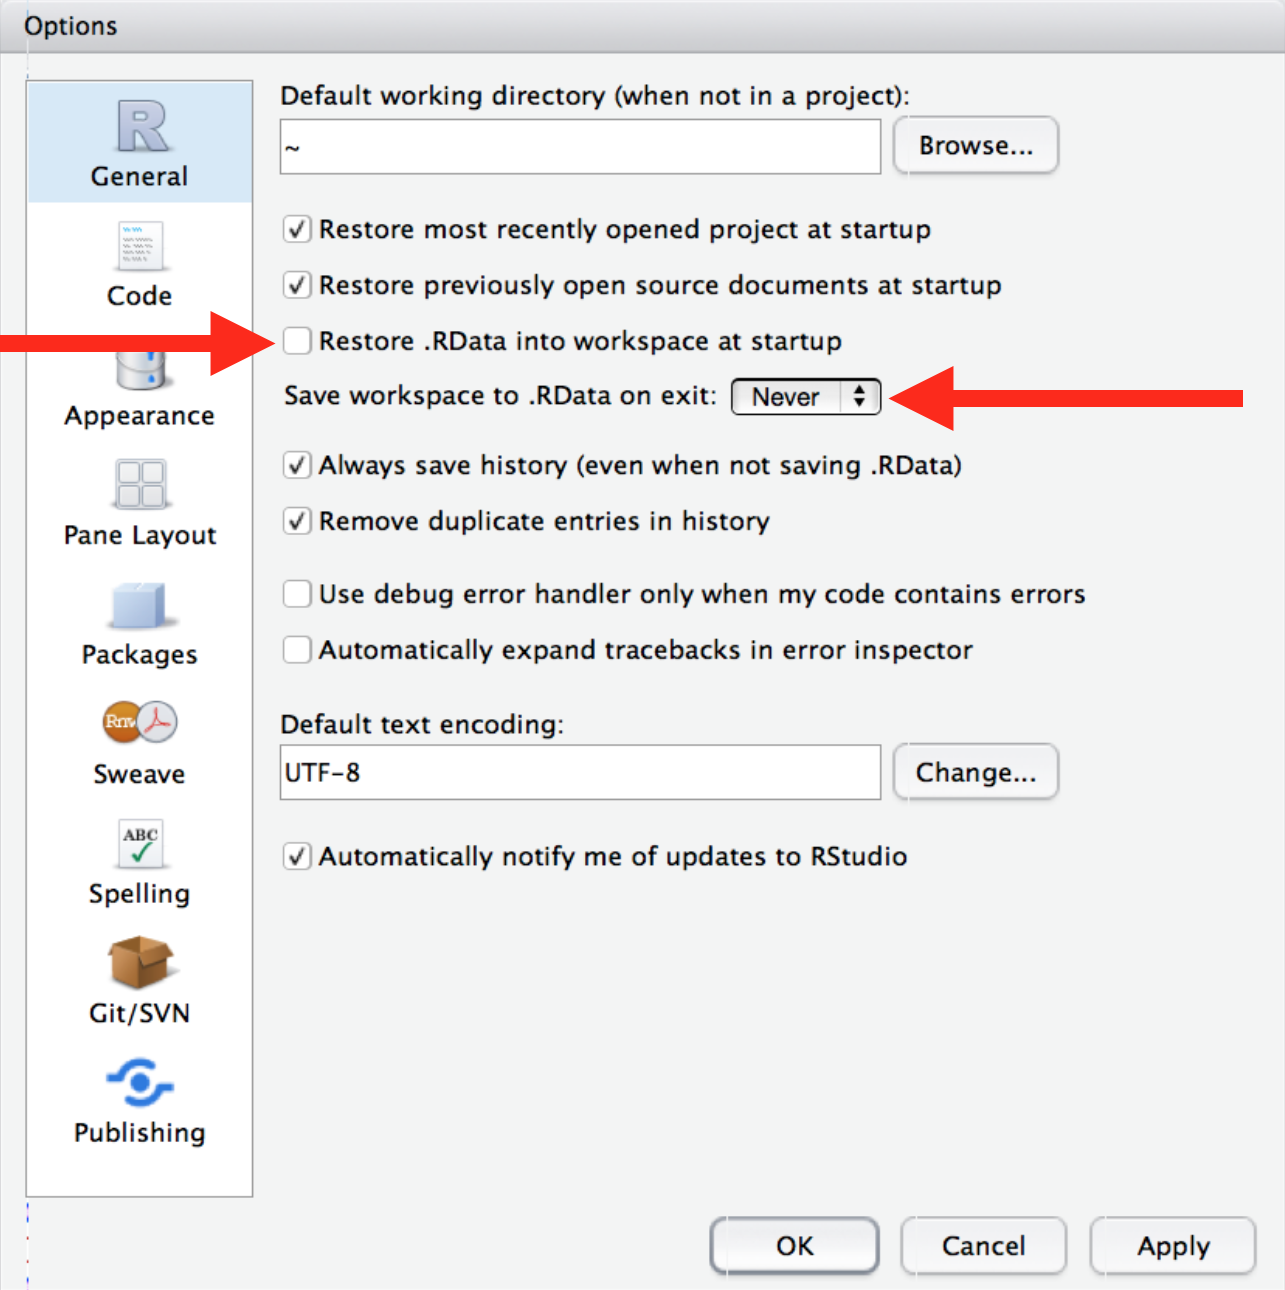
\includegraphics[width=0.7\linewidth]{img/rstudio-workspace} \end{center}

This will cause you some short-term pain, because now when you restart
RStudio, it will not remember the results of the code that you ran last
time. But this short-term pain will save you long-term agony, because it
will force you to capture all important interactions in your scripts.

\subsection{Working Directories and
Paths}\label{working-directories-and-paths}

Like many programming languages, R has a powerful notion of the
\textbf{working directory}. This is where R looks for files that you ask
it to load and where it will put any files that you ask it to save.

RStudio shows your current working directory at the top of the console.
You can print this out in R code by running \texttt{getwd()}:

\begin{Shaded}
\begin{Highlighting}[]
\KeywordTok{getwd}\NormalTok{()}
\CommentTok{#> [1] "/Users/rochelleterman/Desktop/materials"}
\end{Highlighting}
\end{Shaded}

I do not recommend it, but you can set the working directory from within
R:

\begin{Shaded}
\begin{Highlighting}[]
\KeywordTok{setwd}\NormalTok{(}\StringTok{"/path/to/my/CoolProject"}\NormalTok{)}
\end{Highlighting}
\end{Shaded}

The command above prints out a \textbf{path} to your working directory.
Think of a path as an address. Paths are incredibly important in
programming, but they can be a little tricky. Let's go into a bit more
detail.

\subsubsection*{Absolute Paths}\label{absolute-paths}
\addcontentsline{toc}{subsubsection}{Absolute Paths}

Absolute paths are paths that point to the same place regardless of your
current working directory. They always start with the \textbf{root
directory} that holds everything else on your computer.

\begin{itemize}
\tightlist
\item
  In Windows, absolute paths start with a drive letter (e.g.,
  \texttt{C:}) or two backslashes (e.g.,
  \texttt{\textbackslash{}\textbackslash{}servername}).
\item
  In Mac/Linux, they start with a slash \texttt{/}. This is the leading
  slash in \texttt{/users/rterman}.
\end{itemize}

Inside the root directory are several other directories, which we call
\textbf{subdirectories}. We know that the directory
\texttt{/home/rterman} is stored inside \texttt{/home} because
\texttt{/home} is the first part of its name. Similarly, we know that
\texttt{/home} is stored inside the root directory \texttt{/} because
its name begins with \texttt{/}.

Notice that there are two meanings for the \texttt{/} character:

\begin{itemize}
\tightlist
\item
  When it appears \emph{at the front} of a file or directory name, it
  refers to the root directory.
\item
  When it appears \emph{inside} a name, it is just a separator.
\end{itemize}

\subsubsection*{Mac/Linux vs.~Windows}\label{maclinux-vs.windows}
\addcontentsline{toc}{subsubsection}{Mac/Linux vs.~Windows}

There are two basic styles of paths: Mac/Linux and Windows. The main
difference is how they separate the components of the path. Mac and
Linux use slashes (e.g., \texttt{plots/diamonds.pdf}), whereas Windows
uses backslashes (e.g., \texttt{plots\textbackslash{}diamonds.pdf}).

R can work with either type, no matter what platform you are currently
using. Unfortunately, backslashes mean something special to R, and to
get a single backslash in the path, you need to type two backslashes!
That makes life frustrating, so I recommend always using the Linux/Mac
style with forward slashes.

\subsubsection*{Home Directory}\label{home-directory}
\addcontentsline{toc}{subsubsection}{Home Directory}

Sometimes you will see a \texttt{\textasciitilde{}} character in a path.

\begin{itemize}
\tightlist
\item
  In Mac/Linux, the \texttt{\textasciitilde{}} is a convenient shortcut
  to your \textbf{home directory} (\texttt{/users/rterman}).
\item
  Windows does not really have the notion of a home directory, so it
  usually points to your documents directory
  (\texttt{C:\textbackslash{}Documents} and
  \texttt{Settings\textbackslash{}rterman}).
\end{itemize}

\subsubsection*{Absolute vs.~Relative
Paths}\label{absolute-vs.relative-paths}
\addcontentsline{toc}{subsubsection}{Absolute vs.~Relative Paths}

You should try not to use absolute paths in your scripts, because they
hinder sharing: no one else will have exactly the same directory
configuration as you. Another way to direct R to something is to give it
a \textbf{relative path}.

Relative paths point to something relative to where you are (i.e.,
relative to your working directory) rather than from the root of the
file system. For example, if your current working directory is
\texttt{/home/rterman}, then the relative path \texttt{data/un.csv}
directs to the full absolute path: \texttt{/home/rterman/data/un.csv}.

\subsection{R Projects}\label{r-projects}

As a beginning R user, it is OK to let your home directory, documents
directory, or any other weird directory on your computer be R's working
directory.

But from this point forward, you should be organizing your projects into
dedicated subdirectories containing all the files associated with a
project --- input data, R scripts, results, figures\ldots{}

This is such a common practice that RStudio has built-in support for
this via \textbf{projects}.

Let's make a project together. Click
\texttt{File\ \textgreater{}\ New\ Project}, then:

\begin{center}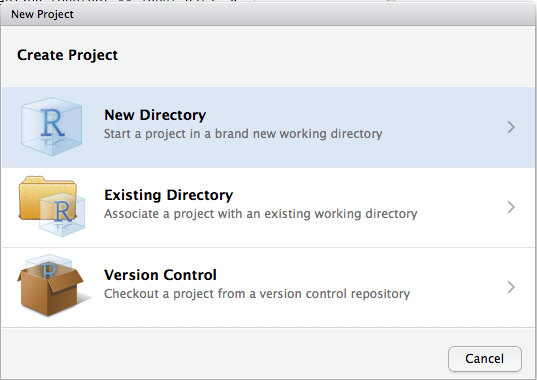
\includegraphics[width=0.7\linewidth]{img/rstudio-project-1} \end{center}

Think carefully about which subdirectory you put the project in. If you
do not store it somewhere sensible, it will be hard to find in the
future!

Once this process is complete, you will get a new RStudio project. Check
that the ``home'' directory of your project is the current working
directory:

\begin{Shaded}
\begin{Highlighting}[]
\KeywordTok{getwd}\NormalTok{()}
\CommentTok{#> [1] "/Users/rochelleterman/Desktop/materials"}
\end{Highlighting}
\end{Shaded}

Now whenever you refer to a file with a relative path, R will look for
the file there.

Go ahead and create a new R script and save it inside the project
folder.

Quit RStudio. Inspect the folder associated with your project --- notice
the .Rproj file. Double-click that file to re-open the project. Notice
you get back to where you left off: it is the same working directory and
command history, and all the files you were working on are still open.
Because you followed my instructions above, however, you will have a
completely fresh environment, guaranteeing that you are starting with a
clean slate.

\subsection{File Organization}\label{file-organization}

You should be saving all your files associated with your project in one
directory. Here is a basic organization structure that I recommend:

\begin{Shaded}
\begin{Highlighting}[]
\NormalTok{~~~}
\NormalTok{masters_thesis:}
\NormalTok{  masters_thesis.Rproj}
\NormalTok{  01_Clean.R}
\NormalTok{  02_Model.R}
\NormalTok{  03_Visualizations.R}
\NormalTok{  Data/}
\BaseNTok{    raw/}
\BaseNTok{      un-raw.csv}
\BaseNTok{      worldbank-raw.csv}
\BaseNTok{    cleaned/}
\BaseNTok{      country-year.csv}
\NormalTok{  Results:}
\BaseNTok{    regressions}
\BaseNTok{      h1.txt}
\BaseNTok{      h2.txt}
\BaseNTok{    figures}
\BaseNTok{      bivariate.pdf}
\BaseNTok{      bar_plot.pdf}
\NormalTok{~~~}
\end{Highlighting}
\end{Shaded}

Here are some important tips:

\begin{itemize}
\tightlist
\item
  Read raw data from the \texttt{Data} subdirectory. Do not ever change
  or overwrite the raw data!
\item
  Export cleaned and altered data into a separate subdirectory.
\item
  Write separate scripts for each stage in the research pipeline. Keep
  scripts short and focused on one main purpose. If a script gets too
  long, that might be a sign you need to split it up.
\item
  Write scripts that reproduce your results and figures, which you can
  save in the \texttt{Results} subdirectory.
\end{itemize}

\section{Importing and Exporting}\label{importing-and-exporting}

\subsection{Where Is My Data?}\label{where-is-my-data}

To start, you first need to know where your data lives. Sometimes, the
data is stored as a file on your computer, e.g., CSV, Excel, SPSS, or
some other file type. When the data is on your computer, we say the data
is stored \textbf{locally}.

Data can also be stored externally on the Internet, in a package, or
obtained through other sources. For example, some R packages contain
datasets (like the \texttt{gapminder} package). Later in this course, we
will discuss how to obtain data from web APIs and websites. For now, the
rest of the unit discusses data that is stored \textbf{locally}.

\subsection{Data Storage}\label{data-storage}

Ideally, your data should be stored in a certain file format. I
recommend a CSV (comma separated value) file, which formats spreadsheet
(rectangular) data in a plain-text format. CSV files are plain-text and
can be read into almost any statistical software program, including R.
Try to avoid Excel files if you can.

Here are some other tips:

\begin{itemize}
\tightlist
\item
  When working with spreadsheets, the first row is usually reserved for
  the header, while the first column is used to identify the sampling
  unit (\textbf{unique identifier}, or \textbf{key}).
\item
  Avoid file names and variable names with blank spaces. This can cause
  errors when reading in data.
\item
  If you want to concatenate words, insert a \texttt{.} or \texttt{\_}
  in between two words instead of a space.
\item
  Short names are prefered over longer names.
\item
  Try to avoid using names that contain symbols such as \texttt{?},
  \texttt{\$},\texttt{\%}, \texttt{\^{}}, \texttt{\&}, \texttt{*},
  \texttt{(}, \texttt{)}, \texttt{-}, \texttt{\#}, \texttt{?},
  \texttt{,}, \texttt{\textless{}}, \texttt{\textgreater{}}, \texttt{/},
  \texttt{\textbar{}}, \texttt{\textbackslash{}}, \texttt{{[}}
  ,\texttt{{]}},\texttt{\{}, and \texttt{\}}.
\item
  make sure that any missing values in your dataset are indicated with
  \texttt{NA} or blank fields (do not use 99 or 77).
\end{itemize}

\subsection{Importing Data}\label{importing-data}

\subsubsection*{Find Paths First}\label{find-paths-first}
\addcontentsline{toc}{subsubsection}{Find Paths First}

In order to import (or read) data into R, you first have to know where
it is and how to find it.

First, remember that you will need to know the \emph{current working
directory} so that you know where R is looking for files. If you are
using R Projects, that working directory will be the top-level directory
of the project.

Second, you will need to know where the data file is relative to your
working directory. If it is stored in the \texttt{Data/raw/} folder, the
relative path to your file will be \texttt{Data/raw/file-name.csv}

\subsubsection*{Reading Tabular Data}\label{reading-tabular-data}
\addcontentsline{toc}{subsubsection}{Reading Tabular Data}

The workhorse for reading into a dataframe is \emph{read.table()}, which
allows any separator (CSV, tab-delimited, etc.). \emph{read.csv()} is a
special case of \emph{read.table()} for CSV files.

The basic formula is:

\begin{Shaded}
\begin{Highlighting}[]
\CommentTok{# Basic CSV read: Import data with header row, values separated by ",", decimals as "."}
\NormalTok{mydataset <-}\StringTok{ }\KeywordTok{read.csv}\NormalTok{(}\DataTypeTok{file=}\StringTok{"  "}\NormalTok{, }\DataTypeTok{stringsAsFactors=}\NormalTok{)}
\end{Highlighting}
\end{Shaded}

Here is a practical example using the PolityIV dataset:

\begin{Shaded}
\begin{Highlighting}[]
\CommentTok{# Import polity}
\NormalTok{polity <-}\StringTok{ }\KeywordTok{read.csv}\NormalTok{(}\StringTok{"data/polity_sub.csv"}\NormalTok{, }\DataTypeTok{stringsAsFactors =}\NormalTok{ F)}
\KeywordTok{head}\NormalTok{(polity)}
\CommentTok{#>       country year polity2}
\CommentTok{#> 1 Afghanistan 1800      -6}
\CommentTok{#> 2 Afghanistan 1801      -6}
\CommentTok{#> 3 Afghanistan 1802      -6}
\CommentTok{#> 4 Afghanistan 1803      -6}
\CommentTok{#> 5 Afghanistan 1804      -6}
\CommentTok{#> 6 Afghanistan 1805      -6}
\end{Highlighting}
\end{Shaded}

We use \texttt{stringsAsFactors\ =\ F} in order to treat text columns as
character vectors, not as factors. If we do not set this, the default is
that all non-numerical columns will be encoded as factors. This behavior
usually makes poor sense and is due to historical reasons. At one point
in time, factors were faster than character vectors, so R's
\texttt{read.table()} set the default to read in text as factors.

\texttt{read.table()} has a number of other options:

\begin{Shaded}
\begin{Highlighting}[]
\CommentTok{# For importing tabular data with maximum customizability}
\NormalTok{mydataset <-}\StringTok{ }\KeywordTok{read.table}\NormalTok{(}\DataTypeTok{file=}\NormalTok{, }\DataTypeTok{header=}\NormalTok{, }\DataTypeTok{sep=}\NormalTok{, }\DataTypeTok{quote=}\NormalTok{, }\DataTypeTok{dec=}\NormalTok{, }\DataTypeTok{fill=}\NormalTok{, }\DataTypeTok{stringsAsFactors=}\NormalTok{)}
\end{Highlighting}
\end{Shaded}

You might also see commands like \texttt{read\_csv()} (notice the
underscore instead of a period). This is the \texttt{tidyverse} version
of \texttt{read.csv()} and accomplishes the same task.

\subsubsection*{Reading Excel Files}\label{reading-excel-files}
\addcontentsline{toc}{subsubsection}{Reading Excel Files}

Do not use Microsoft Excel files (.xls or .xlsx). But if you must:

\begin{Shaded}
\begin{Highlighting}[]
\CommentTok{# Make sure you have installed the tidyverse suite (only necessary one time)}
\CommentTok{# install.packages("tidyverse") # Not Run}

\CommentTok{# Load the "readxl" package (necessary every new R session)}
\KeywordTok{library}\NormalTok{(readxl)}
\end{Highlighting}
\end{Shaded}

\texttt{read\_excel()} reads both .xls and .xlsx files, and detects the
format from the extension.

\begin{Shaded}
\begin{Highlighting}[]
\CommentTok{# Basic call}
\NormalTok{mydataset <-}\StringTok{ }\KeywordTok{read_excel}\NormalTok{(}\DataTypeTok{path =}\NormalTok{ , }\DataTypeTok{sheet =} \StringTok{")}
\end{Highlighting}
\end{Shaded}

Here is a real example:

\begin{Shaded}
\begin{Highlighting}[]
\CommentTok{# Example with .xlsx (single sheet)}
\NormalTok{air <-}\StringTok{ }\KeywordTok{read_excel}\NormalTok{(}\StringTok{"data/airline_small.xlsx"}\NormalTok{, }\DataTypeTok{sheet =} \DecValTok{1}\NormalTok{) }
\NormalTok{air[}\DecValTok{1}\OperatorTok{:}\DecValTok{5}\NormalTok{, }\DecValTok{1}\OperatorTok{:}\DecValTok{5}\NormalTok{]}
\CommentTok{#> # A tibble: 5 x 5}
\CommentTok{#>    Year Month DayofMonth DayOfWeek DepTime}
\CommentTok{#>   <dbl> <dbl>      <dbl>     <dbl> <chr>  }
\CommentTok{#> 1  2005    11         22         2 1700   }
\CommentTok{#> 2  2008     1         31         4 2216   }
\CommentTok{#> 3  2005     7         17         7 905    }
\CommentTok{#> 4  2008     9         23         2 859    }
\CommentTok{#> 5  2005     3          5         6 827}
\end{Highlighting}
\end{Shaded}

\subsubsection*{Reading Stata (.dta)
Files}\label{reading-stata-.dta-files}
\addcontentsline{toc}{subsubsection}{Reading Stata (.dta) Files}

There are many ways to read .dta files into R. I recommend using
\texttt{haven}, because it is part of the \texttt{tidyverse}.

\begin{Shaded}
\begin{Highlighting}[]
\KeywordTok{library}\NormalTok{(haven)}
\NormalTok{air.dta <-}\StringTok{ }\KeywordTok{read_dta}\NormalTok{(}\StringTok{"data/airline_small.dta"}\NormalTok{) }
\NormalTok{air[}\DecValTok{1}\OperatorTok{:}\DecValTok{5}\NormalTok{, }\DecValTok{1}\OperatorTok{:}\DecValTok{5}\NormalTok{]}
\CommentTok{#> # A tibble: 5 x 5}
\CommentTok{#>    Year Month DayofMonth DayOfWeek DepTime}
\CommentTok{#>   <dbl> <dbl>      <dbl>     <dbl> <chr>  }
\CommentTok{#> 1  2005    11         22         2 1700   }
\CommentTok{#> 2  2008     1         31         4 2216   }
\CommentTok{#> 3  2005     7         17         7 905    }
\CommentTok{#> 4  2008     9         23         2 859    }
\CommentTok{#> 5  2005     3          5         6 827}
\end{Highlighting}
\end{Shaded}

\subsubsection*{For Really Big Data}\label{for-really-big-data}
\addcontentsline{toc}{subsubsection}{For Really Big Data}

If you have really big data, \texttt{read.csv()} will be too slow. In
these cases, check out the following options:

\begin{enumerate}
\def\labelenumi{\arabic{enumi})}
\tightlist
\item
  \texttt{read\_csv()} in the \texttt{readr} package is a faster, more
  helpful drop-in replacement for \texttt{read.csv()} that plays well
  with \texttt{tidyverse} packages (discussed in future lessons).
\item
  The \texttt{data.table} package is great for reading and manipulating
  large datasets (orders of gigabytes or 10s of gigabytes).
\end{enumerate}

\subsection{Exporting Data}\label{exporting-data}

You should never go from raw data to results in one script. Typically,
you will want to import raw data, clean it, and then export that cleaned
dataset onto your computer. That cleaned dataset will then be imported
into another script for analysis, in a modular fashion.

To export (or write) data from R onto your computer, you can create
individual CSV files or export many data objects into an \texttt{.RData}
object.

\subsubsection*{\texorpdfstring{Writing a \texttt{csv}
Spreadsheet}{Writing a csv Spreadsheet}}\label{writing-a-csv-spreadsheet}
\addcontentsline{toc}{subsubsection}{Writing a \texttt{csv} Spreadsheet}

To export an individual dataframe as a spreadsheet, use
\texttt{write.csv()}

\begin{Shaded}
\begin{Highlighting}[]
\CommentTok{# Basic call}
\KeywordTok{write.csv}\NormalTok{(}\DataTypeTok{x =}\NormalTok{ , }\DataTypeTok{file =}\NormalTok{ , }\DataTypeTok{row.names =}\NormalTok{ , }\DataTypeTok{col.names =}\NormalTok{)}
\end{Highlighting}
\end{Shaded}

Let's write the \texttt{air} dataset as a CSV:

\begin{Shaded}
\begin{Highlighting}[]
\CommentTok{# Basic call}
\KeywordTok{write.csv}\NormalTok{(air, }\StringTok{"data/airlines.csv"}\NormalTok{, }\DataTypeTok{row.names =}\NormalTok{ F)}
\end{Highlighting}
\end{Shaded}

\subsubsection*{Packaging Data into
.RData}\label{packaging-data-into-.rdata}
\addcontentsline{toc}{subsubsection}{Packaging Data into .RData}

Sometimes, it is helpful to write several dataframes at once to be used
in later analysis. To do so, we use the \texttt{save()} function to
create one file containing many R data objects:

\begin{Shaded}
\begin{Highlighting}[]
\CommentTok{# Basic call}
\KeywordTok{save}\NormalTok{(..., }\DataTypeTok{file =}\NormalTok{ )}
\end{Highlighting}
\end{Shaded}

Here is how we can write both \texttt{air} and \texttt{polity} into one
file:

\begin{Shaded}
\begin{Highlighting}[]
\KeywordTok{save}\NormalTok{(air, polity, }\DataTypeTok{file =} \StringTok{"data/datasets.RData"}\NormalTok{)}
\end{Highlighting}
\end{Shaded}

We can then read these datasets back into R using \texttt{load()}:

\begin{Shaded}
\begin{Highlighting}[]
\CommentTok{# Clear environment}
\KeywordTok{rm}\NormalTok{(}\DataTypeTok{list=}\KeywordTok{ls}\NormalTok{())}

\CommentTok{# Load datasets}
\KeywordTok{load}\NormalTok{(}\StringTok{"data/datasets.RData"}\NormalTok{)}
\end{Highlighting}
\end{Shaded}

\subsubsection*{Acknowledgements}\label{acknowledgements}
\addcontentsline{toc}{subsubsection}{Acknowledgements}

This page is, in part, derived from the following sources:

\begin{enumerate}
\def\labelenumi{\arabic{enumi}.}
\item
  \href{https://r4ds.had.co.nz}{R for Data Science}, licensed under
  \href{https://creativecommons.org/licenses/by-nc-nd/3.0/us/}{Creative
  Commons Attribution-NonCommercial-NoDerivs 3.0}.
\item
  \href{https://web.stanford.edu/~gentzkow/research/CodeAndData.pdf}{Gentzkow,
  Matthew and Jesse M. Shapiro. 2014. Code and Data for the Social
  Sciences: A Practitioner's Guide.}.
\end{enumerate}

\chapter{Data Transformation}\label{data-transformation}

\section{Introduction to Data}\label{introduction-to-data}

The upcoming weeks will be focused on using R for data cleaning and
analysis. Let's first get on the same page with some terms:

\begin{itemize}
\item
  A \textbf{variable} is a quantity, quality, or property that you can
  measure.
\item
  An \textbf{observation} is a set of measurements for the same unit. An
  observation will contain several values, each associated with a
  different variable. I will sometimes refer to an observation as a
  \textbf{data point} or an \textbf{element}.
\item
  A \textbf{value} is the state of a variable for a particular
  observation.
\item
  \textbf{Tabular data} are a set of values, each associated with a
  variable and an observation. Tabular data have rows (observations) and
  columns (variables). Tabular data are also called \textbf{rectangular}
  data or \textbf{spreadsheets}.
\end{itemize}

\subsection{The Gapminder Dataset}\label{the-gapminder-dataset}

This lesson discusses how to perform basic exploratory data analysis.

For this unit, we will be working with the ``Gapminder'' dataset, which
is an excerpt of the data available at gapminder.org. For each of 142
countries, the data provide values for life expectancy, GDP per capita,
and population, every five years from 1952 to 2007.

\begin{Shaded}
\begin{Highlighting}[]
\KeywordTok{require}\NormalTok{(gapminder)}
\CommentTok{#> Loading required package: gapminder}
\NormalTok{gap <-}\StringTok{ }\NormalTok{gapminder}
\end{Highlighting}
\end{Shaded}

\subsection{Structure and Dimensions}\label{structure-and-dimensions}

By loading the gapminder package, we now have access to a data frame by
the same name. Get an overview of this with \texttt{str()}, which
displays the structure of an object.

\begin{Shaded}
\begin{Highlighting}[]
\KeywordTok{str}\NormalTok{(gap)}
\CommentTok{#> tibble [1,704 x 6] (S3: tbl_df/tbl/data.frame)}
\CommentTok{#>  $ country  : Factor w/ 142 levels "Afghanistan",..: 1 1 1 1 1 1 1 1 1 1 ...}
\CommentTok{#>  $ continent: Factor w/ 5 levels "Africa","Americas",..: 3 3 3 3 3 3 3 3 3 3 ...}
\CommentTok{#>  $ year     : int [1:1704] 1952 1957 1962 1967 1972 1977 1982 1987 1992 1997 ...}
\CommentTok{#>  $ lifeExp  : num [1:1704] 28.8 30.3 32 34 36.1 ...}
\CommentTok{#>  $ pop      : int [1:1704] 8425333 9240934 10267083 11537966 13079460 14880372 12881816 13867957 16317921 22227415 ...}
\CommentTok{#>  $ gdpPercap: num [1:1704] 779 821 853 836 740 ...}
\end{Highlighting}
\end{Shaded}

\texttt{str()} will provide a sensible description of almost anything
and, worst case, nothing bad can actually happen. When in doubt, just
\texttt{str()} some of the recently created objects to get some ideas
about what to do next.

We could print the \texttt{gapminder} object itself to screen. However,
if you have used R before, you might be reluctant to do this, because
large datasets just fill up your Console and provide very little
insight.

The \texttt{head} function displays the first 6 rows of any dataframe.

\begin{Shaded}
\begin{Highlighting}[]
\KeywordTok{head}\NormalTok{(gap)}
\CommentTok{#> # A tibble: 6 x 6}
\CommentTok{#>   country     continent  year lifeExp      pop gdpPercap}
\CommentTok{#>   <fct>       <fct>     <int>   <dbl>    <int>     <dbl>}
\CommentTok{#> 1 Afghanistan Asia       1952    28.8  8425333      779.}
\CommentTok{#> 2 Afghanistan Asia       1957    30.3  9240934      821.}
\CommentTok{#> 3 Afghanistan Asia       1962    32.0 10267083      853.}
\CommentTok{#> 4 Afghanistan Asia       1967    34.0 11537966      836.}
\CommentTok{#> 5 Afghanistan Asia       1972    36.1 13079460      740.}
\CommentTok{#> 6 Afghanistan Asia       1977    38.4 14880372      786.}
\end{Highlighting}
\end{Shaded}

Here are some more common ways to query info from a dataframe:

\begin{Shaded}
\begin{Highlighting}[]
\CommentTok{# Get number of rows and columns:}
\KeywordTok{dim}\NormalTok{(gap)}
\CommentTok{#> [1] 1704    6}

\CommentTok{# See column names:}
\KeywordTok{names}\NormalTok{(gap)}
\CommentTok{#> [1] "country"   "continent" "year"      "lifeExp"   "pop"       "gdpPercap"}

\CommentTok{# A statistical overview can be obtained with summary():}
\KeywordTok{summary}\NormalTok{(gap)}
\CommentTok{#>         country        continent        year         lifeExp    }
\CommentTok{#>  Afghanistan:  12   Africa  :624   Min.   :1952   Min.   :23.6  }
\CommentTok{#>  Albania    :  12   Americas:300   1st Qu.:1966   1st Qu.:48.2  }
\CommentTok{#>  Algeria    :  12   Asia    :396   Median :1980   Median :60.7  }
\CommentTok{#>  Angola     :  12   Europe  :360   Mean   :1980   Mean   :59.5  }
\CommentTok{#>  Argentina  :  12   Oceania : 24   3rd Qu.:1993   3rd Qu.:70.8  }
\CommentTok{#>  Australia  :  12                  Max.   :2007   Max.   :82.6  }
\CommentTok{#>  (Other)    :1632                                               }
\CommentTok{#>       pop             gdpPercap     }
\CommentTok{#>  Min.   :6.00e+04   Min.   :   241  }
\CommentTok{#>  1st Qu.:2.79e+06   1st Qu.:  1202  }
\CommentTok{#>  Median :7.02e+06   Median :  3532  }
\CommentTok{#>  Mean   :2.96e+07   Mean   :  7215  }
\CommentTok{#>  3rd Qu.:1.96e+07   3rd Qu.:  9325  }
\CommentTok{#>  Max.   :1.32e+09   Max.   :113523  }
\CommentTok{#> }
\end{Highlighting}
\end{Shaded}

\subsection{Variables}\label{variables-1}

To specify a single variable from a data frame, use the dollar sign
\texttt{\$}. Let's explore the numeric variable for life expectancy.

\begin{Shaded}
\begin{Highlighting}[]
\KeywordTok{head}\NormalTok{(gap}\OperatorTok{$}\NormalTok{lifeExp)}
\CommentTok{#> [1] 28.8 30.3 32.0 34.0 36.1 38.4}
\KeywordTok{summary}\NormalTok{(gap}\OperatorTok{$}\NormalTok{lifeExp)}
\CommentTok{#>    Min. 1st Qu.  Median    Mean 3rd Qu.    Max. }
\CommentTok{#>    23.6    48.2    60.7    59.5    70.8    82.6}
\KeywordTok{hist}\NormalTok{(gap}\OperatorTok{$}\NormalTok{lifeExp)}
\end{Highlighting}
\end{Shaded}

\begin{center}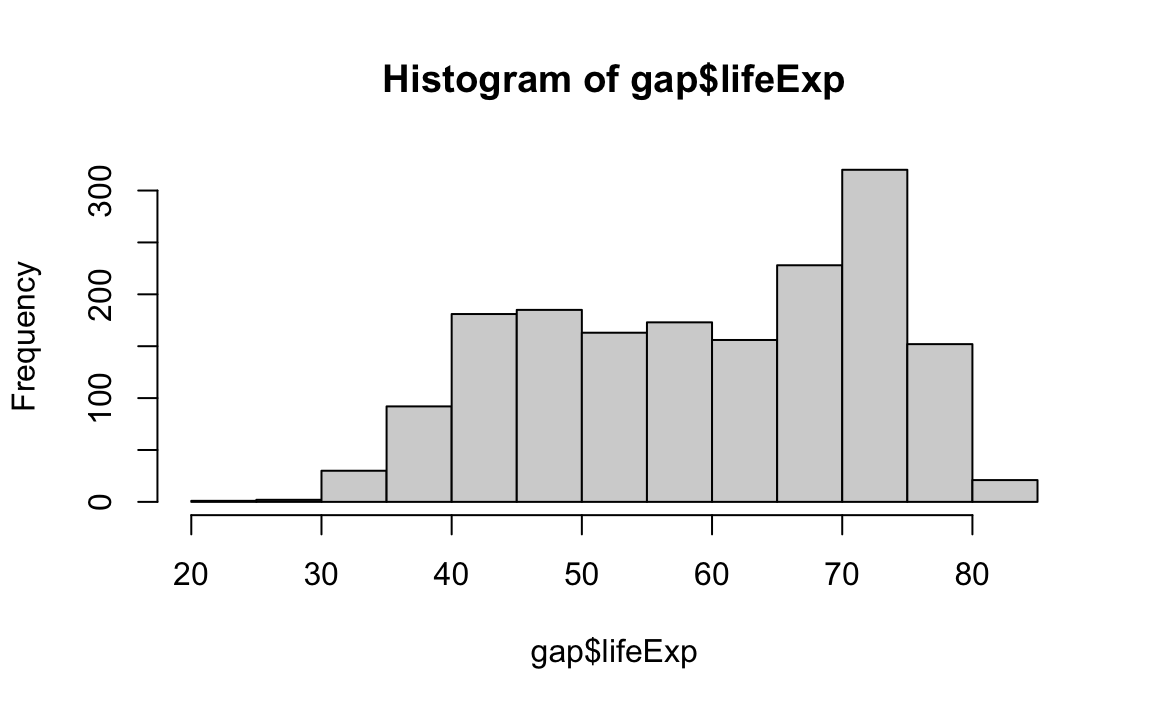
\includegraphics[width=0.7\linewidth]{plsc31101_files/figure-latex/unnamed-chunk-106-1} \end{center}

Data frames -- unlike matrices in R -- can hold variables of different
flavors, such as character data (subject ID or name), quantitative data
(white blood cell count), and categorical information (treated
vs.~untreated).

For example, the \texttt{year} variables is numeric, while the variables
for \texttt{country} and \texttt{continent} hold categorical
information, which is stored as a factor in R.

\begin{Shaded}
\begin{Highlighting}[]
\KeywordTok{summary}\NormalTok{(gap}\OperatorTok{$}\NormalTok{year)}
\CommentTok{#>    Min. 1st Qu.  Median    Mean 3rd Qu.    Max. }
\CommentTok{#>    1952    1966    1980    1980    1993    2007}
\KeywordTok{summary}\NormalTok{(gap}\OperatorTok{$}\NormalTok{country)}
\CommentTok{#>              Afghanistan                  Albania                  Algeria }
\CommentTok{#>                       12                       12                       12 }
\CommentTok{#>                   Angola                Argentina                Australia }
\CommentTok{#>                       12                       12                       12 }
\CommentTok{#>                  Austria                  Bahrain               Bangladesh }
\CommentTok{#>                       12                       12                       12 }
\CommentTok{#>                  Belgium                    Benin                  Bolivia }
\CommentTok{#>                       12                       12                       12 }
\CommentTok{#>   Bosnia and Herzegovina                 Botswana                   Brazil }
\CommentTok{#>                       12                       12                       12 }
\CommentTok{#>                 Bulgaria             Burkina Faso                  Burundi }
\CommentTok{#>                       12                       12                       12 }
\CommentTok{#>                 Cambodia                 Cameroon                   Canada }
\CommentTok{#>                       12                       12                       12 }
\CommentTok{#> Central African Republic                     Chad                    Chile }
\CommentTok{#>                       12                       12                       12 }
\CommentTok{#>                    China                 Colombia                  Comoros }
\CommentTok{#>                       12                       12                       12 }
\CommentTok{#>         Congo, Dem. Rep.              Congo, Rep.               Costa Rica }
\CommentTok{#>                       12                       12                       12 }
\CommentTok{#>            Cote d'Ivoire                  Croatia                     Cuba }
\CommentTok{#>                       12                       12                       12 }
\CommentTok{#>           Czech Republic                  Denmark                 Djibouti }
\CommentTok{#>                       12                       12                       12 }
\CommentTok{#>       Dominican Republic                  Ecuador                    Egypt }
\CommentTok{#>                       12                       12                       12 }
\CommentTok{#>              El Salvador        Equatorial Guinea                  Eritrea }
\CommentTok{#>                       12                       12                       12 }
\CommentTok{#>                 Ethiopia                  Finland                   France }
\CommentTok{#>                       12                       12                       12 }
\CommentTok{#>                    Gabon                   Gambia                  Germany }
\CommentTok{#>                       12                       12                       12 }
\CommentTok{#>                    Ghana                   Greece                Guatemala }
\CommentTok{#>                       12                       12                       12 }
\CommentTok{#>                   Guinea            Guinea-Bissau                    Haiti }
\CommentTok{#>                       12                       12                       12 }
\CommentTok{#>                 Honduras         Hong Kong, China                  Hungary }
\CommentTok{#>                       12                       12                       12 }
\CommentTok{#>                  Iceland                    India                Indonesia }
\CommentTok{#>                       12                       12                       12 }
\CommentTok{#>                     Iran                     Iraq                  Ireland }
\CommentTok{#>                       12                       12                       12 }
\CommentTok{#>                   Israel                    Italy                  Jamaica }
\CommentTok{#>                       12                       12                       12 }
\CommentTok{#>                    Japan                   Jordan                    Kenya }
\CommentTok{#>                       12                       12                       12 }
\CommentTok{#>         Korea, Dem. Rep.              Korea, Rep.                   Kuwait }
\CommentTok{#>                       12                       12                       12 }
\CommentTok{#>                  Lebanon                  Lesotho                  Liberia }
\CommentTok{#>                       12                       12                       12 }
\CommentTok{#>                    Libya               Madagascar                   Malawi }
\CommentTok{#>                       12                       12                       12 }
\CommentTok{#>                 Malaysia                     Mali               Mauritania }
\CommentTok{#>                       12                       12                       12 }
\CommentTok{#>                Mauritius                   Mexico                 Mongolia }
\CommentTok{#>                       12                       12                       12 }
\CommentTok{#>               Montenegro                  Morocco               Mozambique }
\CommentTok{#>                       12                       12                       12 }
\CommentTok{#>                  Myanmar                  Namibia                    Nepal }
\CommentTok{#>                       12                       12                       12 }
\CommentTok{#>              Netherlands              New Zealand                Nicaragua }
\CommentTok{#>                       12                       12                       12 }
\CommentTok{#>                    Niger                  Nigeria                   Norway }
\CommentTok{#>                       12                       12                       12 }
\CommentTok{#>                     Oman                 Pakistan                   Panama }
\CommentTok{#>                       12                       12                       12 }
\CommentTok{#>                  (Other) }
\CommentTok{#>                      516}
\KeywordTok{summary}\NormalTok{(gap}\OperatorTok{$}\NormalTok{contintent)}
\CommentTok{#> Warning: Unknown or uninitialised column: `contintent`.}
\CommentTok{#> Length  Class   Mode }
\CommentTok{#>      0   NULL   NULL}
\end{Highlighting}
\end{Shaded}

Sometimes we need to do some basic checking for the number of
observations or types of observations in our dataset. To do this quickly
and easily, \texttt{table()} is our friend.

Let's look at the number of observations first by region, and then by
both region and year:

\begin{Shaded}
\begin{Highlighting}[]
\KeywordTok{table}\NormalTok{(gap}\OperatorTok{$}\NormalTok{continent)}
\CommentTok{#> }
\CommentTok{#>   Africa Americas     Asia   Europe  Oceania }
\CommentTok{#>      624      300      396      360       24}
\KeywordTok{table}\NormalTok{(gap}\OperatorTok{$}\NormalTok{continent, gap}\OperatorTok{$}\NormalTok{year)}
\CommentTok{#>           }
\CommentTok{#>            1952 1957 1962 1967 1972 1977 1982 1987 1992 1997 2002 2007}
\CommentTok{#>   Africa     52   52   52   52   52   52   52   52   52   52   52   52}
\CommentTok{#>   Americas   25   25   25   25   25   25   25   25   25   25   25   25}
\CommentTok{#>   Asia       33   33   33   33   33   33   33   33   33   33   33   33}
\CommentTok{#>   Europe     30   30   30   30   30   30   30   30   30   30   30   30}
\CommentTok{#>   Oceania     2    2    2    2    2    2    2    2    2    2    2    2}
\end{Highlighting}
\end{Shaded}

We can even divide by the total number of rows to get proportion,
percent, etc.:

\begin{Shaded}
\begin{Highlighting}[]
\KeywordTok{table}\NormalTok{(gap}\OperatorTok{$}\NormalTok{continent)}\OperatorTok{/}\KeywordTok{nrow}\NormalTok{(gap)}
\CommentTok{#> }
\CommentTok{#>   Africa Americas     Asia   Europe  Oceania }
\CommentTok{#>   0.3662   0.1761   0.2324   0.2113   0.0141}
\KeywordTok{table}\NormalTok{(gap}\OperatorTok{$}\NormalTok{continent)}\OperatorTok{/}\KeywordTok{nrow}\NormalTok{(gap)}\OperatorTok{*}\DecValTok{100}
\CommentTok{#> }
\CommentTok{#>   Africa Americas     Asia   Europe  Oceania }
\CommentTok{#>    36.62    17.61    23.24    21.13     1.41}
\end{Highlighting}
\end{Shaded}

\subsection{Challenges}\label{challenges-5}

\subsubsection*{Challenge 1.}\label{challenge-1.-2}
\addcontentsline{toc}{subsubsection}{Challenge 1.}

Read the \texttt{polity\_sub} dataset in the \texttt{Data}
sub-directory.

\subsubsection*{Challenge 2.}\label{challenge-2.-1}
\addcontentsline{toc}{subsubsection}{Challenge 2.}

Report the number and name of each variable in the dataset.

\subsubsection*{Challenge 3.}\label{challenge-3.-1}
\addcontentsline{toc}{subsubsection}{Challenge 3.}

What is the mean \texttt{polity2} score in the dataset?

\subsubsection*{Challenge 4.}\label{challenge-4.}
\addcontentsline{toc}{subsubsection}{Challenge 4.}

What is the range of the \texttt{polity2} variable?

\subsubsection*{Challenge 5.}\label{challenge-5.}
\addcontentsline{toc}{subsubsection}{Challenge 5.}

How many unique countries are in the dataset?

\section{\texorpdfstring{Introduction to
\texttt{dplyr}}{Introduction to dplyr}}\label{introduction-to-dplyr}

\subsection{\texorpdfstring{\texttt{tidyverse}}{tidyverse}}\label{tidyverse}

\begin{quote}
It is often said that 80\% of data analysis is spent on the process of
cleaning and preparing the data.
\end{quote}

\begin{quote}
Dasu and Johnson, 2003
\end{quote}

For most applied researchers, data preparation usually involves 3 main
steps:

\begin{enumerate}
\def\labelenumi{\arabic{enumi}.}
\tightlist
\item
  \textbf{Transforming} data frames, e.g., filtering, summarizing, and
  conducting calculations across groups.
\item
  \textbf{Tidying} data into the appropriate format.
\item
  \textbf{Merging} or linking several datasets to create a bigger
  dataset.
\end{enumerate}

The \href{https://www.tidyverse.org/}{\texttt{tidyverse}} is a suite of
packages designed specifically to help with these steps. These are by no
means the only packages out there for data wrangling, but they are
increasingly popular for their readable, straightforward syntax and
sensible default behaviors.

In this chapter, we are going to focus on how to use the \texttt{dplyr}
package for data transformation tasks.

For this unit, we will be working with the Gapminder dataset again.

\begin{Shaded}
\begin{Highlighting}[]
\KeywordTok{library}\NormalTok{(tidyverse)}
\KeywordTok{library}\NormalTok{(gapminder)}

\NormalTok{gap <-}\StringTok{ }\NormalTok{gapminder}
\KeywordTok{head}\NormalTok{(gap)}
\CommentTok{#> # A tibble: 6 x 6}
\CommentTok{#>   country     continent  year lifeExp      pop gdpPercap}
\CommentTok{#>   <fct>       <fct>     <int>   <dbl>    <int>     <dbl>}
\CommentTok{#> 1 Afghanistan Asia       1952    28.8  8425333      779.}
\CommentTok{#> 2 Afghanistan Asia       1957    30.3  9240934      821.}
\CommentTok{#> 3 Afghanistan Asia       1962    32.0 10267083      853.}
\CommentTok{#> 4 Afghanistan Asia       1967    34.0 11537966      836.}
\CommentTok{#> 5 Afghanistan Asia       1972    36.1 13079460      740.}
\CommentTok{#> 6 Afghanistan Asia       1977    38.4 14880372      786.}
\end{Highlighting}
\end{Shaded}

\subsection{\texorpdfstring{Why
\texttt{dplyr}?}{Why dplyr?}}\label{why-dplyr}

If you have ever used base R before, you know the following will
calculate the mean GDP per capita within each region:

\begin{Shaded}
\begin{Highlighting}[]
\KeywordTok{mean}\NormalTok{(gap}\OperatorTok{$}\NormalTok{gdpPercap[gap}\OperatorTok{$}\NormalTok{continent }\OperatorTok{==}\StringTok{ "Africa"}\NormalTok{])}
\CommentTok{#> [1] 2194}
\KeywordTok{mean}\NormalTok{(gap}\OperatorTok{$}\NormalTok{gdpPercap[gap}\OperatorTok{$}\NormalTok{continent }\OperatorTok{==}\StringTok{ "Americas"}\NormalTok{])}
\CommentTok{#> [1] 7136}
\KeywordTok{mean}\NormalTok{(gap}\OperatorTok{$}\NormalTok{gdpPercap[gap}\OperatorTok{$}\NormalTok{continent }\OperatorTok{==}\StringTok{ "Asia"}\NormalTok{])}
\CommentTok{#> [1] 7902}
\end{Highlighting}
\end{Shaded}

But this is not ideal because it involves a fair bit of repetition.
Repeating yourself will cost you time, both now and later, and
potentially introduce some nasty bugs.

Luckily, the
\href{https://cran.r-project.org/web/packages/dplyr/dplyr.pdf}{\texttt{dplyr}}
package provides a number of very useful functions for manipulating
dataframes. These functions will save you time by reducing repetition.
As an added bonus, you might even find the \texttt{dplyr} grammar easier
to read.

Here, we are going to cover 7 of the most commonly used \texttt{dplyr}
functions. We will also cover pipes (\texttt{\%\textgreater{}\%}), which
are used to combine those functions.

\begin{enumerate}
\def\labelenumi{\arabic{enumi}.}
\tightlist
\item
  \texttt{select()}
\item
  \texttt{filter()}
\item
  \texttt{mutate()}
\item
  \texttt{arrange()}
\item
  \texttt{count()}
\item
  \texttt{group\_by()}
\item
  \texttt{summarize()}
\item
  \texttt{mutate()}
\end{enumerate}

If you have not installed \texttt{tidyverse}, please do so now:

\begin{Shaded}
\begin{Highlighting}[]
\CommentTok{# not run}
\CommentTok{# install.packages('tidyverse')}
\KeywordTok{require}\NormalTok{(tidyverse)}
\end{Highlighting}
\end{Shaded}

\subsection{\texorpdfstring{Select Columns with
\texttt{select}}{Select Columns with select}}\label{select-columns-with-select}

Imagine that we have just received the Gapminder dataset, but are only
interested in a few variables in it. We could use the \texttt{select()}
function to keep only the variables we select.

\begin{Shaded}
\begin{Highlighting}[]
\NormalTok{year_country_gdp <-}\StringTok{ }\KeywordTok{select}\NormalTok{(gap, year, country, gdpPercap)}
\KeywordTok{head}\NormalTok{(year_country_gdp)}
\CommentTok{#> # A tibble: 6 x 3}
\CommentTok{#>    year country     gdpPercap}
\CommentTok{#>   <int> <fct>           <dbl>}
\CommentTok{#> 1  1952 Afghanistan      779.}
\CommentTok{#> 2  1957 Afghanistan      821.}
\CommentTok{#> 3  1962 Afghanistan      853.}
\CommentTok{#> 4  1967 Afghanistan      836.}
\CommentTok{#> 5  1972 Afghanistan      740.}
\CommentTok{#> 6  1977 Afghanistan      786.}
\end{Highlighting}
\end{Shaded}

\begin{center}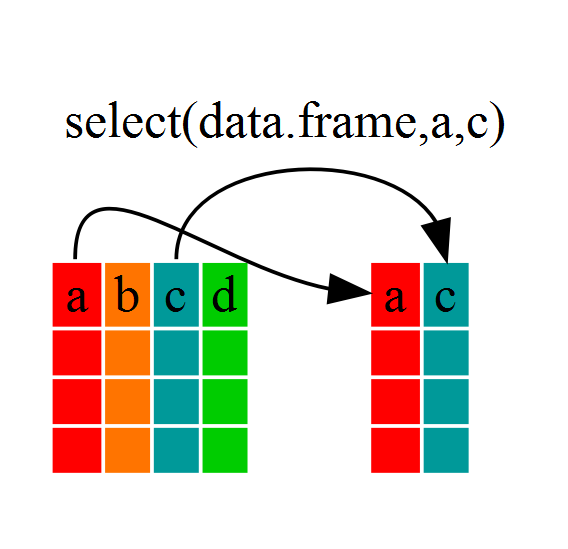
\includegraphics[width=0.7\linewidth]{img/dplyr-fig1} \end{center}

If we open up \texttt{year\_country\_gdp}, we will see that it only
contains the \texttt{year}, \texttt{country}, and \texttt{gdpPercap}.
This is equivalent to the base R subsetting function:

\begin{Shaded}
\begin{Highlighting}[]
\NormalTok{year_country_gdp_base <-}\StringTok{ }\NormalTok{gap[,}\KeywordTok{c}\NormalTok{(}\StringTok{"year"}\NormalTok{, }\StringTok{"country"}\NormalTok{, }\StringTok{"gdpPercap"}\NormalTok{)]}
\KeywordTok{head}\NormalTok{(year_country_gdp)}
\CommentTok{#> # A tibble: 6 x 3}
\CommentTok{#>    year country     gdpPercap}
\CommentTok{#>   <int> <fct>           <dbl>}
\CommentTok{#> 1  1952 Afghanistan      779.}
\CommentTok{#> 2  1957 Afghanistan      821.}
\CommentTok{#> 3  1962 Afghanistan      853.}
\CommentTok{#> 4  1967 Afghanistan      836.}
\CommentTok{#> 5  1972 Afghanistan      740.}
\CommentTok{#> 6  1977 Afghanistan      786.}
\end{Highlighting}
\end{Shaded}

\subsection{The Pipe}\label{the-pipe}

\begin{center}
\includegraphics[width=0.7\linewidth]{img/pipe} \end{center}

Above, we used what is called `normal' grammar, but the strengths of
\texttt{dplyr} lie in combining several functions using \emph{pipes}.

In typical base R code, a simple operation might be written like:

\begin{Shaded}
\begin{Highlighting}[]
\CommentTok{# NOT run}
\NormalTok{cupcakes <-}\StringTok{ }\KeywordTok{bake}\NormalTok{(}\KeywordTok{pour}\NormalTok{(}\KeywordTok{mix}\NormalTok{(ingredients)))}
\end{Highlighting}
\end{Shaded}

A computer has no trouble understanding this, and your cupcakes will be
made just fine, but a person has to read right to left to understand the
order of operations -- the opposite of how most Western languages are
read -- making it harder to understand what is being done!

To be more readable without pipes, we might break up this code into
intermediate objects:

\begin{Shaded}
\begin{Highlighting}[]
\NormalTok{## NOT run}
\NormalTok{batter <-}\StringTok{ }\KeywordTok{mix}\NormalTok{(ingredients)}
\NormalTok{muffin_tin <-}\StringTok{ }\KeywordTok{pour}\NormalTok{(batter)}
\NormalTok{cupcakes <-}\StringTok{ }\KeywordTok{bake}\NormalTok{(muffin_tin)}
\end{Highlighting}
\end{Shaded}

But this can clutter our environment with a lot of variables that are
not very useful to us. Plus, these variables are often named very
similar things (e.g., step, step1, step2\ldots{}), which can lead to
confusion and the creation of hard-to-track-down bugs.

\subsubsection*{Enter the Pipe\ldots{}}\label{enter-the-pipe}
\addcontentsline{toc}{subsubsection}{Enter the Pipe\ldots{}}

The \emph{pipe} makes it easier to read code by laying out operations
from left to right -- each line can be read like a line of a recipe for
the perfect data frame!

Pipes take the input on the left side of the \texttt{\%\textgreater{}\%}
symbol and pass it in as the first argument to the function on the right
side.

With pipes, our cupcake example might be written like:

\begin{Shaded}
\begin{Highlighting}[]
\NormalTok{## NOT run}
\NormalTok{cupcakes <-}\StringTok{ }\NormalTok{ingredients }\OperatorTok\StringTok{ }
\StringTok{  }\KeywordTok{mix}\NormalTok{() }\OperatorTok\StringTok{ }
\StringTok{  }\KeywordTok{pour}\NormalTok{() }\OperatorTok\StringTok{ }
\StringTok{  }\KeywordTok{bake}\NormalTok{()}
\end{Highlighting}
\end{Shaded}

\subsubsection*{\texorpdfstring{\texttt{select} \& Pipe
(\texttt{\%\textgreater{}\%})}{select \& Pipe (\%\textgreater{}\%)}}\label{select-pipe}
\addcontentsline{toc}{subsubsection}{\texttt{select} \& Pipe
(\texttt{\%\textgreater{}\%})}

Let's repeat what we did above with the Gapminder dataset using pipes:

\begin{Shaded}
\begin{Highlighting}[]
\NormalTok{year_country_gdp <-}\StringTok{ }\NormalTok{gap }\OperatorTok\StringTok{ }
\StringTok{  }\KeywordTok{select}\NormalTok{(year, country, gdpPercap)}
\end{Highlighting}
\end{Shaded}

First, we summon the gapminder data frame and pass it on to the next
step using the pipe symbol \texttt{\%\textgreater{}\%}.

The second step is the \texttt{select()} function. In this case, we do
not specify which data object we use in the call to \texttt{select()}
since we have piped it in from the previous line.

\subsubsection*{Tips for Piping}\label{tips-for-piping}
\addcontentsline{toc}{subsubsection}{Tips for Piping}

\begin{enumerate}
\def\labelenumi{\arabic{enumi}.}
\item
  Remember that you do not assign anything within the pipes --- that is,
  you should not use \texttt{\textless{}-} inside the piped operation.
  Only use \texttt{\textless{}-} at the beginning of your code if you
  want to save the output.
\item
  Remember to add the pipe \texttt{\%\textgreater{}\%} at the end of
  each line involved in the piped operation. A good rule of thumb: since
  RStudio will automatically indent lines of code that are part of a
  piped operation, if the line is not indented, it probably has not been
  added to the pipe. If you have an error in a piped operation, always
  check to make sure the pipe is connected as you expect.
\item
  In RStudio, the hotkey for the pipe is \texttt{Ctrl\ +\ Shift\ +\ M}.
\end{enumerate}

\subsection{\texorpdfstring{Filter Rows with
\texttt{filter}}{Filter Rows with filter}}\label{filter-rows-with-filter}

Now let's say we are only interested in African countries. We can
combine \texttt{select} and \texttt{filter} to select only the
observations where \texttt{continent} is \texttt{Africa}.

\begin{Shaded}
\begin{Highlighting}[]
\NormalTok{year_country_gdp_africa <-}\StringTok{ }\NormalTok{gap }\OperatorTok
\StringTok{    }\KeywordTok{filter}\NormalTok{(continent }\OperatorTok{==}\StringTok{ "Africa"}\NormalTok{) }\OperatorTok
\StringTok{    }\KeywordTok{select}\NormalTok{(year, country, gdpPercap)}
\end{Highlighting}
\end{Shaded}

As with last time, first we pass the gapminder dataframe to the
\texttt{filter()} function, then we pass the filtered version of the
Gapminder dataframe to the \texttt{select()} function.

To clarify, both the \texttt{select} and \texttt{filter} functions
subset the data frame. The difference is that \texttt{select} extracts
certain columns, while \texttt{filter} extracts certain rows.

\textbf{NB}: The order of operations is very important in this case. If
we used \texttt{select} first, \texttt{filter} would not be able to find
the variable \texttt{continent}, since we would have removed it in the
previous step.

\section{\texorpdfstring{More \texttt{dplyr}
functions}{More dplyr functions}}\label{more-dplyr-functions}

\subsubsection*{Where were we?}\label{where-were-we}
\addcontentsline{toc}{subsubsection}{Where were we?}

In the previous lesson, we used two very important verbs and an
operator:

\begin{itemize}
\tightlist
\item
  \texttt{filter()} for subsetting data with row logic.
\item
  \texttt{select()} for subsetting data variable- or column-wise.
\item
  The pipe operator \texttt{\%\textgreater{}\%}, which feeds the LHS as
  the first argument to the expression on the RHS.
\end{itemize}

We also discussed \texttt{dplyr}'s role inside the tidyverse:

\begin{itemize}
\tightlist
\item
  \texttt{dplyr} is a core package in the
  \href{tidyverse-github}{tidyverse} meta-package.
\item
  Since we often make incidental usage of the others, we will load
  \texttt{dplyr} and the others via \texttt{library(tidyverse)}.
\end{itemize}

\begin{Shaded}
\begin{Highlighting}[]
\KeywordTok{library}\NormalTok{(tidyverse)}
\KeywordTok{library}\NormalTok{(gapminder)}

\NormalTok{gap <-}\StringTok{ }\NormalTok{gapminder}
\end{Highlighting}
\end{Shaded}

\subsection{\texorpdfstring{Use \texttt{mutate()} to Add New
Variables}{Use mutate() to Add New Variables}}\label{use-mutate-to-add-new-variables}

Imagine we wanted to recover each country's GDP. After all, the
Gapminder data has a variable for population and GDP per capita. Let's
multiply them together.

\texttt{mutate()} is a function that defines and inserts new variables
into a tibble. You can refer to existing variables by name.

\begin{Shaded}
\begin{Highlighting}[]
\NormalTok{gap }\OperatorTok
\StringTok{  }\KeywordTok{mutate}\NormalTok{(}\DataTypeTok{gdp =}\NormalTok{ pop }\OperatorTok{*}\StringTok{ }\NormalTok{gdpPercap) }\OperatorTok
\StringTok{  }\KeywordTok{head}\NormalTok{()}
\CommentTok{#> # A tibble: 6 x 7}
\CommentTok{#>   country     continent  year lifeExp      pop gdpPercap          gdp}
\CommentTok{#>   <fct>       <fct>     <int>   <dbl>    <int>     <dbl>        <dbl>}
\CommentTok{#> 1 Afghanistan Asia       1952    28.8  8425333      779.  6567086330.}
\CommentTok{#> 2 Afghanistan Asia       1957    30.3  9240934      821.  7585448670.}
\CommentTok{#> 3 Afghanistan Asia       1962    32.0 10267083      853.  8758855797.}
\CommentTok{#> 4 Afghanistan Asia       1967    34.0 11537966      836.  9648014150.}
\CommentTok{#> 5 Afghanistan Asia       1972    36.1 13079460      740.  9678553274.}
\CommentTok{#> 6 Afghanistan Asia       1977    38.4 14880372      786. 11697659231.}
\end{Highlighting}
\end{Shaded}

We can add multiple columns in one call:

\begin{Shaded}
\begin{Highlighting}[]
\NormalTok{gap }\OperatorTok
\StringTok{  }\KeywordTok{mutate}\NormalTok{(}\DataTypeTok{gdp =}\NormalTok{ pop }\OperatorTok{*}\StringTok{ }\NormalTok{gdpPercap,}
         \DataTypeTok{log_gdp =} \KeywordTok{log}\NormalTok{(gdp)) }\OperatorTok
\StringTok{  }\KeywordTok{head}\NormalTok{()}
\CommentTok{#> # A tibble: 6 x 8}
\CommentTok{#>   country     continent  year lifeExp      pop gdpPercap          gdp log_gdp}
\CommentTok{#>   <fct>       <fct>     <int>   <dbl>    <int>     <dbl>        <dbl>   <dbl>}
\CommentTok{#> 1 Afghanistan Asia       1952    28.8  8425333      779.  6567086330.    22.6}
\CommentTok{#> 2 Afghanistan Asia       1957    30.3  9240934      821.  7585448670.    22.7}
\CommentTok{#> 3 Afghanistan Asia       1962    32.0 10267083      853.  8758855797.    22.9}
\CommentTok{#> 4 Afghanistan Asia       1967    34.0 11537966      836.  9648014150.    23.0}
\CommentTok{#> 5 Afghanistan Asia       1972    36.1 13079460      740.  9678553274.    23.0}
\CommentTok{#> 6 Afghanistan Asia       1977    38.4 14880372      786. 11697659231.    23.2}
\end{Highlighting}
\end{Shaded}

\subsection{\texorpdfstring{Use \texttt{arrange()} to Row-order Data in
a Principled
Way}{Use arrange() to Row-order Data in a Principled Way}}\label{use-arrange-to-row-order-data-in-a-principled-way}

\texttt{arrange()} reorders the rows in a data frame. Imagine you wanted
this data ordered by year then country, as opposed to by country then
year.

\begin{Shaded}
\begin{Highlighting}[]
\NormalTok{gap }\OperatorTok
\StringTok{  }\KeywordTok{arrange}\NormalTok{(year, country)}
\CommentTok{#> # A tibble: 1,704 x 6}
\CommentTok{#>   country     continent  year lifeExp      pop gdpPercap}
\CommentTok{#>   <fct>       <fct>     <int>   <dbl>    <int>     <dbl>}
\CommentTok{#> 1 Afghanistan Asia       1952    28.8  8425333      779.}
\CommentTok{#> 2 Albania     Europe     1952    55.2  1282697     1601.}
\CommentTok{#> 3 Algeria     Africa     1952    43.1  9279525     2449.}
\CommentTok{#> 4 Angola      Africa     1952    30.0  4232095     3521.}
\CommentTok{#> 5 Argentina   Americas   1952    62.5 17876956     5911.}
\CommentTok{#> 6 Australia   Oceania    1952    69.1  8691212    10040.}
\CommentTok{#> # ... with 1,698 more rows}
\end{Highlighting}
\end{Shaded}

Or maybe you want just the data from 2007, sorted on life expectancy?

\begin{Shaded}
\begin{Highlighting}[]
\NormalTok{gap }\OperatorTok
\StringTok{  }\KeywordTok{filter}\NormalTok{(year }\OperatorTok{==}\StringTok{ }\DecValTok{2007}\NormalTok{) }\OperatorTok
\StringTok{  }\KeywordTok{arrange}\NormalTok{(lifeExp)}
\CommentTok{#> # A tibble: 142 x 6}
\CommentTok{#>   country      continent  year lifeExp      pop gdpPercap}
\CommentTok{#>   <fct>        <fct>     <int>   <dbl>    <int>     <dbl>}
\CommentTok{#> 1 Swaziland    Africa     2007    39.6  1133066     4513.}
\CommentTok{#> 2 Mozambique   Africa     2007    42.1 19951656      824.}
\CommentTok{#> 3 Zambia       Africa     2007    42.4 11746035     1271.}
\CommentTok{#> 4 Sierra Leone Africa     2007    42.6  6144562      863.}
\CommentTok{#> 5 Lesotho      Africa     2007    42.6  2012649     1569.}
\CommentTok{#> 6 Angola       Africa     2007    42.7 12420476     4797.}
\CommentTok{#> # ... with 136 more rows}
\end{Highlighting}
\end{Shaded}

Oh, you would like to sort on life expectancy in \textbf{desc}ending
order? Then use \texttt{desc()}.

\begin{Shaded}
\begin{Highlighting}[]
\NormalTok{gap }\OperatorTok
\StringTok{  }\KeywordTok{filter}\NormalTok{(year }\OperatorTok{==}\StringTok{ }\DecValTok{2007}\NormalTok{) }\OperatorTok
\StringTok{  }\KeywordTok{arrange}\NormalTok{(}\KeywordTok{desc}\NormalTok{(lifeExp))}
\CommentTok{#> # A tibble: 142 x 6}
\CommentTok{#>   country          continent  year lifeExp       pop gdpPercap}
\CommentTok{#>   <fct>            <fct>     <int>   <dbl>     <int>     <dbl>}
\CommentTok{#> 1 Japan            Asia       2007    82.6 127467972    31656.}
\CommentTok{#> 2 Hong Kong, China Asia       2007    82.2   6980412    39725.}
\CommentTok{#> 3 Iceland          Europe     2007    81.8    301931    36181.}
\CommentTok{#> 4 Switzerland      Europe     2007    81.7   7554661    37506.}
\CommentTok{#> 5 Australia        Oceania    2007    81.2  20434176    34435.}
\CommentTok{#> 6 Spain            Europe     2007    80.9  40448191    28821.}
\CommentTok{#> # ... with 136 more rows}
\end{Highlighting}
\end{Shaded}

I advise that your analyses NEVER rely on rows or variables being in a
specific order. But it is still true that human beings write the code,
and the interactive development process can be much nicer if you reorder
the rows of your data as you go along. Also, once you are preparing
tables for human eyeballs, it is imperative that you step up and take
control of row order.

\subsection{\texorpdfstring{Use \texttt{rename()} to Rename
Variables}{Use rename() to Rename Variables}}\label{use-rename-to-rename-variables}

When I first cleaned this Gapminder excerpt, I was a \texttt{camelCase}
person, but now I am all about \texttt{snake\_case}. So I am vexed by
the variable names I chose when I cleaned this data years ago. Let's
rename some variables!

\begin{Shaded}
\begin{Highlighting}[]
\NormalTok{gap }\OperatorTok
\StringTok{  }\KeywordTok{rename}\NormalTok{(}\DataTypeTok{life_exp =}\NormalTok{ lifeExp,}
         \DataTypeTok{gdp_percap =}\NormalTok{ gdpPercap)}
\CommentTok{#> # A tibble: 1,704 x 6}
\CommentTok{#>   country     continent  year life_exp      pop gdp_percap}
\CommentTok{#>   <fct>       <fct>     <int>    <dbl>    <int>      <dbl>}
\CommentTok{#> 1 Afghanistan Asia       1952     28.8  8425333       779.}
\CommentTok{#> 2 Afghanistan Asia       1957     30.3  9240934       821.}
\CommentTok{#> 3 Afghanistan Asia       1962     32.0 10267083       853.}
\CommentTok{#> 4 Afghanistan Asia       1967     34.0 11537966       836.}
\CommentTok{#> 5 Afghanistan Asia       1972     36.1 13079460       740.}
\CommentTok{#> 6 Afghanistan Asia       1977     38.4 14880372       786.}
\CommentTok{#> # ... with 1,698 more rows}
\end{Highlighting}
\end{Shaded}

\subsection{\texorpdfstring{Use \texttt{select()} to Rename and
Reposition
Variables}{Use select() to Rename and Reposition Variables}}\label{use-select-to-rename-and-reposition-variables}

You have seen the simple use of \texttt{select()}. There are two tricks
you might enjoy:

\begin{enumerate}
\def\labelenumi{\arabic{enumi}.}
\tightlist
\item
  \texttt{select()} can rename the variables you request to keep.
\item
  \texttt{select()} can be used with \texttt{everything()} to hoist a
  variable up to the front of the tibble.
\end{enumerate}

\begin{Shaded}
\begin{Highlighting}[]
\NormalTok{gap }\OperatorTok
\StringTok{  }\KeywordTok{filter}\NormalTok{(country }\OperatorTok{==}\StringTok{ "Burundi"}\NormalTok{, year }\OperatorTok{>}\StringTok{ }\DecValTok{1996}\NormalTok{) }\OperatorTok\StringTok{ }
\StringTok{  }\KeywordTok{select}\NormalTok{(}\DataTypeTok{yr =}\NormalTok{ year, lifeExp, gdpPercap) }\OperatorTok\StringTok{ }
\StringTok{  }\KeywordTok{select}\NormalTok{(gdpPercap, }\KeywordTok{everything}\NormalTok{())}
\CommentTok{#> # A tibble: 3 x 3}
\CommentTok{#>   gdpPercap    yr lifeExp}
\CommentTok{#>       <dbl> <int>   <dbl>}
\CommentTok{#> 1      463.  1997    45.3}
\CommentTok{#> 2      446.  2002    47.4}
\CommentTok{#> 3      430.  2007    49.6}
\end{Highlighting}
\end{Shaded}

\texttt{everything()} is one of several helpers for variable selection.
Read its help to see the rest.

\subsection{\texorpdfstring{Use \texttt{count()} to Count Variable
Quantities}{Use count() to Count Variable Quantities}}\label{use-count-to-count-variable-quantities}

Finally, let's say we want to examine if the number of countries covered
in the Gapminder dataset varies between years. We can use
\texttt{count()} to count the number of observations within a set of
parameters we choose.

Below, we will specify that we want to \texttt{count()} the number of
observations in each year of the dataset:

\begin{Shaded}
\begin{Highlighting}[]
\NormalTok{gap }\OperatorTok
\StringTok{  }\NormalTok{dplyr}\OperatorTok{::}\KeywordTok{count}\NormalTok{(year)}
\CommentTok{#> # A tibble: 12 x 2}
\CommentTok{#>    year     n}
\CommentTok{#>   <int> <int>}
\CommentTok{#> 1  1952   142}
\CommentTok{#> 2  1957   142}
\CommentTok{#> 3  1962   142}
\CommentTok{#> 4  1967   142}
\CommentTok{#> 5  1972   142}
\CommentTok{#> 6  1977   142}
\CommentTok{#> # ... with 6 more rows}
\end{Highlighting}
\end{Shaded}

We can confirm that each year in the dataset contains the same number of
observations. We can use similar syntax to answer other questions: For
example, how many countries in each year have a GDP that is greater than
\$10,000 per capita?

\begin{Shaded}
\begin{Highlighting}[]
\NormalTok{gap }\OperatorTok
\StringTok{  }\KeywordTok{filter}\NormalTok{(gdpPercap }\OperatorTok{>=}\StringTok{ }\DecValTok{10000}\NormalTok{) }\OperatorTok
\StringTok{  }\NormalTok{dplyr}\OperatorTok{::}\KeywordTok{count}\NormalTok{(year) }
\CommentTok{#> # A tibble: 12 x 2}
\CommentTok{#>    year     n}
\CommentTok{#>   <int> <int>}
\CommentTok{#> 1  1952     7}
\CommentTok{#> 2  1957    12}
\CommentTok{#> 3  1962    19}
\CommentTok{#> 4  1967    22}
\CommentTok{#> 5  1972    32}
\CommentTok{#> 6  1977    41}
\CommentTok{#> # ... with 6 more rows}
\end{Highlighting}
\end{Shaded}

\begin{Shaded}
\begin{Highlighting}[]
\KeywordTok{library}\NormalTok{(tidyverse)}
\KeywordTok{library}\NormalTok{(gapminder)}

\NormalTok{gap <-}\StringTok{ }\NormalTok{gapminder}
\KeywordTok{head}\NormalTok{(gap)}
\CommentTok{#> # A tibble: 6 x 6}
\CommentTok{#>   country     continent  year lifeExp      pop gdpPercap}
\CommentTok{#>   <fct>       <fct>     <int>   <dbl>    <int>     <dbl>}
\CommentTok{#> 1 Afghanistan Asia       1952    28.8  8425333      779.}
\CommentTok{#> 2 Afghanistan Asia       1957    30.3  9240934      821.}
\CommentTok{#> 3 Afghanistan Asia       1962    32.0 10267083      853.}
\CommentTok{#> 4 Afghanistan Asia       1967    34.0 11537966      836.}
\CommentTok{#> 5 Afghanistan Asia       1972    36.1 13079460      740.}
\CommentTok{#> 6 Afghanistan Asia       1977    38.4 14880372      786.}
\end{Highlighting}
\end{Shaded}

\section{Calculating across Groups}\label{calculating-across-groups}

A common task you will encounter when working with data is running
calculations on different groups within the data. For instance, what if
we wanted to calculate the mean GDP per capita for each continent?

In base R, you would have to run the \texttt{mean()} function for each
subset of data.

\begin{Shaded}
\begin{Highlighting}[]
\KeywordTok{mean}\NormalTok{(gap}\OperatorTok{$}\NormalTok{gdpPercap[gap}\OperatorTok{$}\NormalTok{continent }\OperatorTok{==}\StringTok{ "Africa"}\NormalTok{])}
\CommentTok{#> [1] 2194}
\KeywordTok{mean}\NormalTok{(gap}\OperatorTok{$}\NormalTok{gdpPercap[gap}\OperatorTok{$}\NormalTok{continent }\OperatorTok{==}\StringTok{ "Americas"}\NormalTok{])}
\CommentTok{#> [1] 7136}
\KeywordTok{mean}\NormalTok{(gap}\OperatorTok{$}\NormalTok{gdpPercap[gap}\OperatorTok{$}\NormalTok{continent }\OperatorTok{==}\StringTok{ "Asia"}\NormalTok{])}
\CommentTok{#> [1] 7902}
\KeywordTok{mean}\NormalTok{(gap}\OperatorTok{$}\NormalTok{gdpPercap[gap}\OperatorTok{$}\NormalTok{continent }\OperatorTok{==}\StringTok{ "Europe"}\NormalTok{])}
\CommentTok{#> [1] 14469}
\KeywordTok{mean}\NormalTok{(gap}\OperatorTok{$}\NormalTok{gdpPercap[gap}\OperatorTok{$}\NormalTok{continent }\OperatorTok{==}\StringTok{ "Oceania"}\NormalTok{])}
\CommentTok{#> [1] 18622}
\end{Highlighting}
\end{Shaded}

That is a lot of repetition! To make matters worse, what if we wanted to
add these values to our original data frame as a new column? We would
have to write something like this:

\begin{Shaded}
\begin{Highlighting}[]
\NormalTok{gap}\OperatorTok{$}\NormalTok{mean.continent.GDP <-}\StringTok{ }\OtherTok{NA}
\NormalTok{gap}\OperatorTok{$}\NormalTok{mean.continent.GDP[gap}\OperatorTok{$}\NormalTok{continent }\OperatorTok{==}\StringTok{ "Africa"}\NormalTok{] <-}\StringTok{ }\KeywordTok{mean}\NormalTok{(gap}\OperatorTok{$}\NormalTok{gdpPercap[gap}\OperatorTok{$}\NormalTok{continent }\OperatorTok{==}\StringTok{ "Africa"}\NormalTok{])}
\NormalTok{gap}\OperatorTok{$}\NormalTok{mean.continent.GDP[gap}\OperatorTok{$}\NormalTok{continent }\OperatorTok{==}\StringTok{ "Americas"}\NormalTok{] <-}\StringTok{ }\KeywordTok{mean}\NormalTok{(gap}\OperatorTok{$}\NormalTok{gdpPercap[gap}\OperatorTok{$}\NormalTok{continent }\OperatorTok{==}\StringTok{ "Americas"}\NormalTok{])}
\NormalTok{gap}\OperatorTok{$}\NormalTok{mean.continent.GDP[gap}\OperatorTok{$}\NormalTok{continent }\OperatorTok{==}\StringTok{ "Asia"}\NormalTok{] <-}\StringTok{ }\KeywordTok{mean}\NormalTok{(gap}\OperatorTok{$}\NormalTok{gdpPercap[gap}\OperatorTok{$}\NormalTok{continent }\OperatorTok{==}\StringTok{ "Asia"}\NormalTok{])}
\NormalTok{gap}\OperatorTok{$}\NormalTok{mean.continent.GDP[gap}\OperatorTok{$}\NormalTok{continent }\OperatorTok{==}\StringTok{ "Europe"}\NormalTok{] <-}\StringTok{ }\KeywordTok{mean}\NormalTok{(gap}\OperatorTok{$}\NormalTok{gdpPercap[gap}\OperatorTok{$}\NormalTok{continent }\OperatorTok{==}\StringTok{ "Europe"}\NormalTok{])}
\NormalTok{gap}\OperatorTok{$}\NormalTok{mean.continent.GDP[gap}\OperatorTok{$}\NormalTok{continent }\OperatorTok{==}\StringTok{ "Oceania"}\NormalTok{] <-}\StringTok{ }\KeywordTok{mean}\NormalTok{(gap}\OperatorTok{$}\NormalTok{gdpPercap[gap}\OperatorTok{$}\NormalTok{continent }\OperatorTok{==}\StringTok{ "Oceania"}\NormalTok{])}
\end{Highlighting}
\end{Shaded}

You can see how this can get pretty tedious, especially if we want to
calculate more complicated or refined statistics. We could use loops or
apply functions, but these can be difficult, slow, and error-prone.

\subsubsection*{Split-apply-combine}\label{split-apply-combine}
\addcontentsline{toc}{subsubsection}{Split-apply-combine}

The abstract problem we are encountering here is know as
``split-apply-combine'':

\begin{center}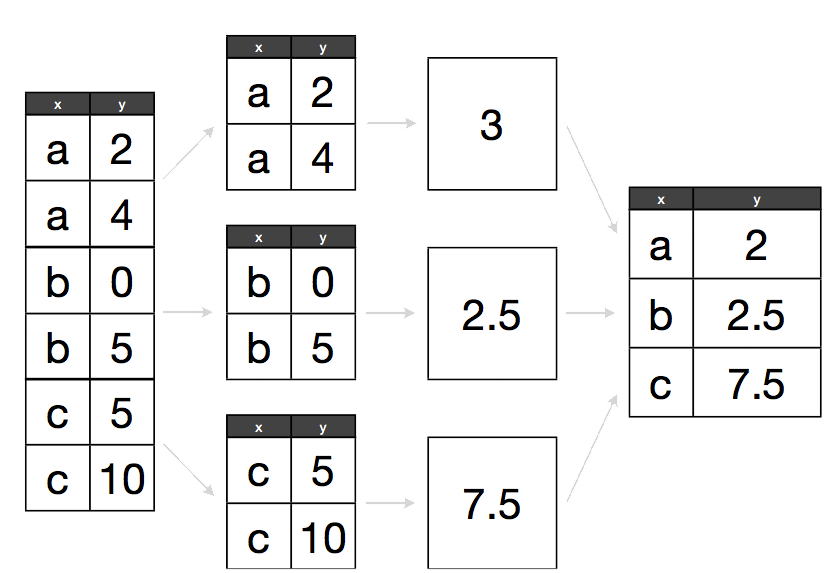
\includegraphics[width=0.7\linewidth]{img/splitapply} \end{center}

We want to \emph{split} our data into groups (in this case, continents),
\emph{apply} some calculations on that group, then \emph{combine} the
results together afterwards.

Luckily, \texttt{dplyr} offers a much cleaner, straight-forward solution
to this problem.

First, let's remove the column we just made:

\begin{Shaded}
\begin{Highlighting}[]
\NormalTok{gap <-}\StringTok{ }\NormalTok{gapminder}
\end{Highlighting}
\end{Shaded}

\subsection{\texorpdfstring{Use \texttt{group\_by} to Create a Grouped
Data}{Use group\_by to Create a Grouped Data}}\label{use-group_by-to-create-a-grouped-data}

We have already seen how \texttt{filter()} can help us select
observations that meet certain criteria (in the above:
\texttt{continent\ ==\ "Africa"}). More helpful, however, is the
\texttt{group\_by()} function, which will essentially use every unique
criterium that we could have used in \texttt{filter()}.

A \texttt{grouped\_df} can be thought of as a \texttt{list} where each
item in the \texttt{list} is a \texttt{data.frame} which contains only
the rows that correspond to a particular value for \texttt{continent}
(at least in the example above).

\begin{center}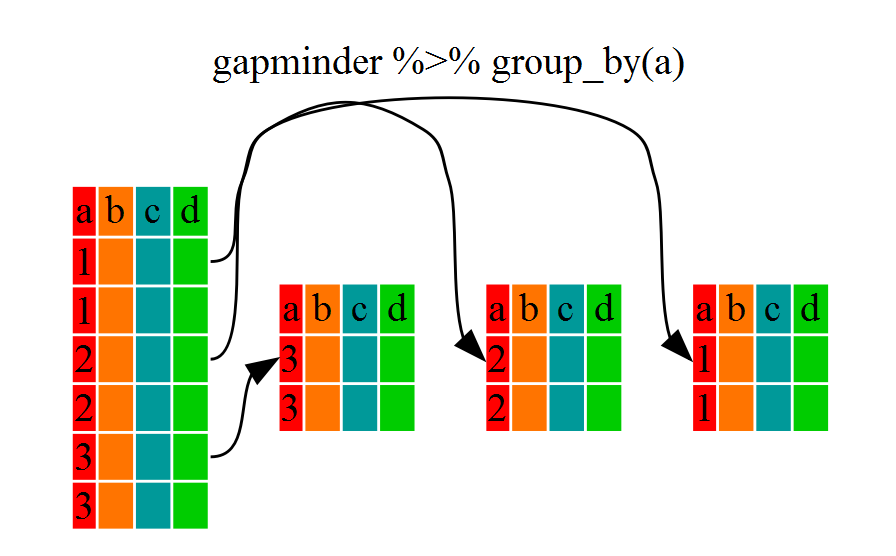
\includegraphics[width=0.7\linewidth]{img/dplyr-fig2} \end{center}

\subsection{\texorpdfstring{Summarize Across Groups with
\texttt{summarize}}{Summarize Across Groups with summarize}}\label{summarize-across-groups-with-summarize}

\texttt{group\_by()} on its own is not particularly interesting. It is
much more exciting used in conjunction with the \texttt{summarize()}
function.

This will allow us to create new variable(s) by applying transformations
to variables in each of our groups (continent-specific data frames).

In other words, using the \texttt{group\_by()} function, we split our
original data frame into multiple pieces, to which we then apply summary
functions (e.g., \texttt{mean()} or \texttt{sd()}) within
\texttt{summarize()}.

The output is a new data frame reduced in size, with one row per group.

\begin{Shaded}
\begin{Highlighting}[]
\NormalTok{gap }\OperatorTok
\StringTok{  }\KeywordTok{group_by}\NormalTok{(continent) }\OperatorTok
\StringTok{  }\KeywordTok{summarize}\NormalTok{(}\DataTypeTok{mean_gdpPercap =} \KeywordTok{mean}\NormalTok{(gdpPercap)) }
\CommentTok{#> `summarise()` ungrouping output (override with `.groups` argument)}
\CommentTok{#> # A tibble: 5 x 2}
\CommentTok{#>   continent mean_gdpPercap}
\CommentTok{#>   <fct>              <dbl>}
\CommentTok{#> 1 Africa             2194.}
\CommentTok{#> 2 Americas           7136.}
\CommentTok{#> 3 Asia               7902.}
\CommentTok{#> 4 Europe            14469.}
\CommentTok{#> 5 Oceania           18622.}
\end{Highlighting}
\end{Shaded}

\begin{center}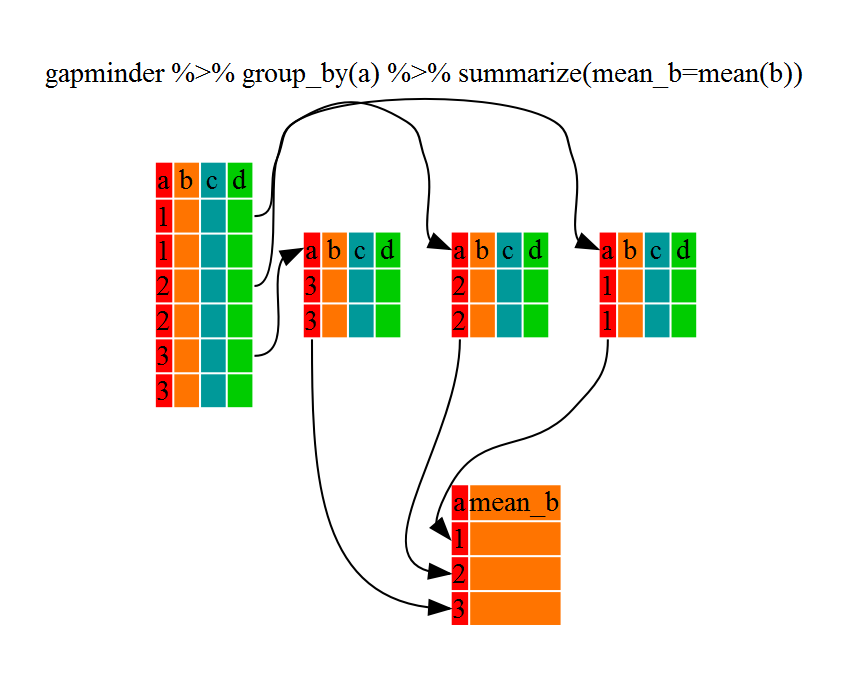
\includegraphics[width=0.7\linewidth]{img/dplyr-fig3} \end{center}

That allowed us to calculate the mean \texttt{gdpPercap} for each
continent.

But it gets even better -- the function \texttt{group\_by()} allows us
to group by multiple variables. Let's group by \texttt{year} and
\texttt{continent}:

\begin{Shaded}
\begin{Highlighting}[]
\NormalTok{gap }\OperatorTok
\StringTok{  }\KeywordTok{group_by}\NormalTok{(continent, year) }\OperatorTok
\StringTok{  }\KeywordTok{summarize}\NormalTok{(}\DataTypeTok{mean_gdpPercap =} \KeywordTok{mean}\NormalTok{(gdpPercap)) }\OperatorTok
\StringTok{  }\KeywordTok{head}\NormalTok{()}
\CommentTok{#> `summarise()` regrouping output by 'continent' (override with `.groups` argument)}
\CommentTok{#> # A tibble: 6 x 3}
\CommentTok{#> # Groups:   continent [1]}
\CommentTok{#>   continent  year mean_gdpPercap}
\CommentTok{#>   <fct>     <int>          <dbl>}
\CommentTok{#> 1 Africa     1952          1253.}
\CommentTok{#> 2 Africa     1957          1385.}
\CommentTok{#> 3 Africa     1962          1598.}
\CommentTok{#> 4 Africa     1967          2050.}
\CommentTok{#> 5 Africa     1972          2340.}
\CommentTok{#> 6 Africa     1977          2586.}
\end{Highlighting}
\end{Shaded}

That is already quite powerful, but it gets even better! You are not
limited to defining only one new variable in \texttt{summarize()}.

\begin{Shaded}
\begin{Highlighting}[]
\NormalTok{gap }\OperatorTok
\StringTok{  }\KeywordTok{group_by}\NormalTok{(continent, year) }\OperatorTok
\StringTok{  }\KeywordTok{summarize}\NormalTok{(}\DataTypeTok{mean_gdpPercap =} \KeywordTok{mean}\NormalTok{(gdpPercap), }
            \DataTypeTok{sd_gdpPercap =} \KeywordTok{sd}\NormalTok{(gdpPercap),}
            \DataTypeTok{mean_pop =} \KeywordTok{mean}\NormalTok{(pop),}
            \DataTypeTok{sd_pop =} \KeywordTok{sd}\NormalTok{(pop))}
\CommentTok{#> `summarise()` regrouping output by 'continent' (override with `.groups` argument)}
\CommentTok{#> # A tibble: 60 x 6}
\CommentTok{#> # Groups:   continent [5]}
\CommentTok{#>   continent  year mean_gdpPercap sd_gdpPercap mean_pop    sd_pop}
\CommentTok{#>   <fct>     <int>          <dbl>        <dbl>    <dbl>     <dbl>}
\CommentTok{#> 1 Africa     1952          1253.         983. 4570010.  6317450.}
\CommentTok{#> 2 Africa     1957          1385.        1135. 5093033.  7076042.}
\CommentTok{#> 3 Africa     1962          1598.        1462. 5702247.  7957545.}
\CommentTok{#> 4 Africa     1967          2050.        2848. 6447875.  8985505.}
\CommentTok{#> 5 Africa     1972          2340.        3287. 7305376. 10130833.}
\CommentTok{#> 6 Africa     1977          2586.        4142. 8328097. 11585184.}
\CommentTok{#> # ... with 54 more rows}
\end{Highlighting}
\end{Shaded}

\subsection{\texorpdfstring{Add New Variables with
\texttt{mutate}}{Add New Variables with mutate}}\label{add-new-variables-with-mutate}

What if we wanted to add these values to our original data frame instead
of creating a new object?

For this, we can use the \texttt{mutate()} function, which is similar to
\texttt{summarize()} except that it creates new variables in the same
data frame that you pass into it.

\begin{Shaded}
\begin{Highlighting}[]
\NormalTok{gap }\OperatorTok
\StringTok{  }\KeywordTok{group_by}\NormalTok{(continent, year) }\OperatorTok
\StringTok{  }\KeywordTok{mutate}\NormalTok{(}\DataTypeTok{mean_gdpPercap =} \KeywordTok{mean}\NormalTok{(gdpPercap), }
            \DataTypeTok{sd_gdpPercap =} \KeywordTok{sd}\NormalTok{(gdpPercap),}
            \DataTypeTok{mean_pop =} \KeywordTok{mean}\NormalTok{(pop),}
            \DataTypeTok{sd_pop =} \KeywordTok{sd}\NormalTok{(pop))}
\CommentTok{#> # A tibble: 1,704 x 10}
\CommentTok{#> # Groups:   continent, year [60]}
\CommentTok{#>   country continent  year lifeExp    pop gdpPercap mean_gdpPercap sd_gdpPercap}
\CommentTok{#>   <fct>   <fct>     <int>   <dbl>  <int>     <dbl>          <dbl>        <dbl>}
\CommentTok{#> 1 Afghan~ Asia       1952    28.8 8.43e6      779.          5195.       18635.}
\CommentTok{#> 2 Afghan~ Asia       1957    30.3 9.24e6      821.          5788.       19507.}
\CommentTok{#> 3 Afghan~ Asia       1962    32.0 1.03e7      853.          5729.       16416.}
\CommentTok{#> 4 Afghan~ Asia       1967    34.0 1.15e7      836.          5971.       14063.}
\CommentTok{#> 5 Afghan~ Asia       1972    36.1 1.31e7      740.          8187.       19088.}
\CommentTok{#> 6 Afghan~ Asia       1977    38.4 1.49e7      786.          7791.       11816.}
\CommentTok{#> # ... with 1,698 more rows, and 2 more variables: mean_pop <dbl>, sd_pop <dbl>}
\end{Highlighting}
\end{Shaded}

We can also use \texttt{mutate()} to create new variables prior to (or
even after) summarizing the information.

\begin{Shaded}
\begin{Highlighting}[]
\NormalTok{gap }\OperatorTok
\StringTok{  }\KeywordTok{mutate}\NormalTok{(}\DataTypeTok{gdp_billion =}\NormalTok{ gdpPercap}\OperatorTok{*}\NormalTok{pop}\OperatorTok{/}\DecValTok{10}\OperatorTok{^}\DecValTok{9}\NormalTok{) }\OperatorTok
\StringTok{  }\KeywordTok{group_by}\NormalTok{(continent, year) }\OperatorTok
\StringTok{  }\KeywordTok{summarize}\NormalTok{(}\DataTypeTok{mean_gdpPercap =} \KeywordTok{mean}\NormalTok{(gdpPercap),}
            \DataTypeTok{sd_gdpPercap =} \KeywordTok{sd}\NormalTok{(gdpPercap),}
            \DataTypeTok{mean_pop =} \KeywordTok{mean}\NormalTok{(pop),}
            \DataTypeTok{sd_pop =} \KeywordTok{sd}\NormalTok{(pop),}
            \DataTypeTok{mean_gdp_billion =} \KeywordTok{mean}\NormalTok{(gdp_billion),}
            \DataTypeTok{sd_gdp_billion =} \KeywordTok{sd}\NormalTok{(gdp_billion))}
\CommentTok{#> `summarise()` regrouping output by 'continent' (override with `.groups` argument)}
\CommentTok{#> # A tibble: 60 x 8}
\CommentTok{#> # Groups:   continent [5]}
\CommentTok{#>   continent  year mean_gdpPercap sd_gdpPercap mean_pop sd_pop mean_gdp_billion}
\CommentTok{#>   <fct>     <int>          <dbl>        <dbl>    <dbl>  <dbl>            <dbl>}
\CommentTok{#> 1 Africa     1952          1253.         983. 4570010. 6.32e6             5.99}
\CommentTok{#> 2 Africa     1957          1385.        1135. 5093033. 7.08e6             7.36}
\CommentTok{#> 3 Africa     1962          1598.        1462. 5702247. 7.96e6             8.78}
\CommentTok{#> 4 Africa     1967          2050.        2848. 6447875. 8.99e6            11.4 }
\CommentTok{#> 5 Africa     1972          2340.        3287. 7305376. 1.01e7            15.1 }
\CommentTok{#> 6 Africa     1977          2586.        4142. 8328097. 1.16e7            18.7 }
\CommentTok{#> # ... with 54 more rows, and 1 more variable: sd_gdp_billion <dbl>}
\end{Highlighting}
\end{Shaded}

\subsubsection*{\texorpdfstring{\texttt{mutate} vs.
\texttt{summarize}}{mutate vs. summarize}}\label{mutate-vs.-summarize}
\addcontentsline{toc}{subsubsection}{\texttt{mutate} vs.
\texttt{summarize}}

It can be confusing to decide whether to use \texttt{mutate} or
\texttt{summarize}. The key distinction is whether you want the output
to have one row for each group or one row for each row in the original
data frame:

\begin{itemize}
\tightlist
\item
  \texttt{mutate}: Creates new columns with as many rows as the original
  data frame.
\item
  \texttt{summarize}: Creates a data frame with as many rows as groups.
\end{itemize}

Note that if you use an aggregation function such as \texttt{mean()}
within \texttt{mutate()} without using \texttt{group\_by()}, you will
simply do the summary over all the rows of the input data frame.

And if you use an aggregation function such as \texttt{mean()} within
\texttt{summarize()} without using \texttt{group\_by()}, you will simply
create an output data frame with one row (i.e., the whole input data
frame is a single group).

\section{Challenges}\label{challenges-6}

\subsubsection*{Challenge 1.}\label{challenge-1.-3}
\addcontentsline{toc}{subsubsection}{Challenge 1.}

Use \texttt{dplyr} to create a data frame containing the median
\texttt{lifeExp} for each continent.

\subsubsection*{Challenge 2.}\label{challenge-2.-2}
\addcontentsline{toc}{subsubsection}{Challenge 2.}

Use \texttt{dplyr} to add a column to the Gapminder dataset that
contains the total population of the continent of each observation in a
given year. For example, if the first observation is Afghanistan in
1952, the new column would contain the population of Asia in 1952.

\subsubsection*{Challenge 3.}\label{challenge-3.-2}
\addcontentsline{toc}{subsubsection}{Challenge 3.}

Use \texttt{dplyr} to: (a) add a column called \texttt{gdpPercap\_diff}
that contains the difference between the observation's
\texttt{gdpPercap} and the mean \texttt{gdpPercap} of the continent in
that year, and (b) arrange the data frame by the column you just created
in descending order (so that the relatively richest country-years are
listed first).

\textbf{Hint:} You might have to \texttt{ungroup()} before you
\texttt{arrange()}.

\subsubsection*{Acknowledgments}\label{acknowledgments-2}
\addcontentsline{toc}{subsubsection}{Acknowledgments}

Some of the materials in this module were adapted from:

\begin{itemize}
\tightlist
\item
  \href{http://swcarpentry.github.io/r-novice-gapminder/}{Software
  Carpentry}.
\item
  \href{https://github.com/berkeley-scf/r-bootcamp-fall-2019}{R bootcamp
  at UC Berkeley}.
\end{itemize}

\chapter{Tidying Data}\label{tidying-data}

Even before we conduct analyses or calculations, we need to put our data
into the correct format. The goal here is to rearrange a messy dataset
into one that is \textbf{tidy}.

The two most important properties of tidy data are:

\begin{enumerate}
\def\labelenumi{\arabic{enumi})}
\tightlist
\item
  Each column is a variable.
\item
  Each row is an observation.
\end{enumerate}

Tidy data is easier to work with because you have a consistent way of
referring to variables (as column names) and observations (as row
indices). The data then becomes easier to manipulate, visualize, and
model.

For more on the concept of tidy data, read Hadley Wickham's paper
\href{http://vita.had.co.nz/papers/tidy-data.html}{here}.

\section{Wide vs.~Long Formats}\label{wide-vs.long-formats}

\begin{quote}
Tidy datasets are all alike, but every messy dataset is messy in its own
way.
\end{quote}

\begin{quote}
\textbf{Hadley Wickham}
\end{quote}

Tabular datasets can be arranged in many ways. For instance, consider
the data below. Each dataset displays information on heart rates
observed in individuals across three different time periods, but the
data are organized differently in each table.

\begin{Shaded}
\begin{Highlighting}[]
\NormalTok{wide <-}\StringTok{ }\KeywordTok{data.frame}\NormalTok{(}
  \DataTypeTok{name =} \KeywordTok{c}\NormalTok{(}\StringTok{"Wilbur"}\NormalTok{, }\StringTok{"Petunia"}\NormalTok{, }\StringTok{"Gregory"}\NormalTok{),}
  \DataTypeTok{time1 =} \KeywordTok{c}\NormalTok{(}\DecValTok{67}\NormalTok{, }\DecValTok{80}\NormalTok{, }\DecValTok{64}\NormalTok{),}
  \DataTypeTok{time2 =} \KeywordTok{c}\NormalTok{(}\DecValTok{56}\NormalTok{, }\DecValTok{90}\NormalTok{, }\DecValTok{50}\NormalTok{),}
  \DataTypeTok{time3 =} \KeywordTok{c}\NormalTok{(}\DecValTok{70}\NormalTok{, }\DecValTok{67}\NormalTok{, }\DecValTok{101}\NormalTok{)}
\NormalTok{)}
\NormalTok{wide}
\CommentTok{#>      name time1 time2 time3}
\CommentTok{#> 1  Wilbur    67    56    70}
\CommentTok{#> 2 Petunia    80    90    67}
\CommentTok{#> 3 Gregory    64    50   101}

\NormalTok{long <-}\StringTok{ }\KeywordTok{data.frame}\NormalTok{(}
  \DataTypeTok{name =} \KeywordTok{c}\NormalTok{(}\StringTok{"Wilbur"}\NormalTok{, }\StringTok{"Petunia"}\NormalTok{, }\StringTok{"Gregory"}\NormalTok{, }\StringTok{"Wilbur"}\NormalTok{, }\StringTok{"Petunia"}\NormalTok{, }\StringTok{"Gregory"}\NormalTok{, }\StringTok{"Wilbur"}\NormalTok{, }\StringTok{"Petunia"}\NormalTok{, }\StringTok{"Gregory"}\NormalTok{),}
  \DataTypeTok{time =} \KeywordTok{c}\NormalTok{(}\DecValTok{1}\NormalTok{, }\DecValTok{1}\NormalTok{, }\DecValTok{1}\NormalTok{, }\DecValTok{2}\NormalTok{, }\DecValTok{2}\NormalTok{, }\DecValTok{2}\NormalTok{, }\DecValTok{3}\NormalTok{, }\DecValTok{3}\NormalTok{, }\DecValTok{3}\NormalTok{),}
  \DataTypeTok{heartrate =} \KeywordTok{c}\NormalTok{(}\DecValTok{67}\NormalTok{, }\DecValTok{80}\NormalTok{, }\DecValTok{64}\NormalTok{, }\DecValTok{56}\NormalTok{, }\DecValTok{90}\NormalTok{, }\DecValTok{50}\NormalTok{, }\DecValTok{70}\NormalTok{, }\DecValTok{67}\NormalTok{, }\DecValTok{10}\NormalTok{)}
\NormalTok{)}
\NormalTok{long}
\CommentTok{#>      name time heartrate}
\CommentTok{#> 1  Wilbur    1        67}
\CommentTok{#> 2 Petunia    1        80}
\CommentTok{#> 3 Gregory    1        64}
\CommentTok{#> 4  Wilbur    2        56}
\CommentTok{#> 5 Petunia    2        90}
\CommentTok{#> 6 Gregory    2        50}
\CommentTok{#> 7  Wilbur    3        70}
\CommentTok{#> 8 Petunia    3        67}
\CommentTok{#> 9 Gregory    3        10}
\end{Highlighting}
\end{Shaded}

\textbf{Question:} Which one of these do you think is the \emph{tidy}
format?

\textbf{Answer:} The first dataframe (the ``wide'' one) would not be
considered \emph{tidy} because values (i.e., heart rate) are spread
across multiple columns.

We often refer to these different structures as ``long'' vs. ``wide''
formats:

\begin{itemize}
\item
  In the \textbf{``long''} format, you usually have one column for the
  observed variable, and the other columns are ID variables.
\item
  In the \textbf{``wide''} format, each row is often a
  site/subject/patient, and you have multiple observation variables
  containing the same type of data. These can be either repeated
  observations over time or observations of multiple variables (or a mix
  of both). In the case above, we had the same kind of data (heart rate)
  entered across three different columns, corresponding to three
  different time periods.
\end{itemize}

\begin{center}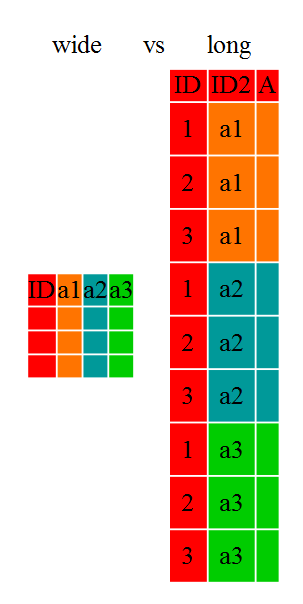
\includegraphics[width=0.7\linewidth]{img/tidyr-fig1} \end{center}

You may find data input in the ``wide'' format to be simpler, and some
other applications may prefer ``wide''-format data. However, many of R's
functions have been designed assuming you have ``long''-format data.

\section{Tidying the Gapminder Data}\label{tidying-the-gapminder-data}

Let's look at the structure of our original \texttt{gapminder}
dataframe:

\begin{Shaded}
\begin{Highlighting}[]
\KeywordTok{library}\NormalTok{(gapminder)}

\NormalTok{gap <-}\StringTok{ }\NormalTok{gapminder}
\KeywordTok{head}\NormalTok{(gap)}
\CommentTok{#> # A tibble: 6 x 6}
\CommentTok{#>   country     continent  year lifeExp      pop gdpPercap}
\CommentTok{#>   <fct>       <fct>     <int>   <dbl>    <int>     <dbl>}
\CommentTok{#> 1 Afghanistan Asia       1952    28.8  8425333      779.}
\CommentTok{#> 2 Afghanistan Asia       1957    30.3  9240934      821.}
\CommentTok{#> 3 Afghanistan Asia       1962    32.0 10267083      853.}
\CommentTok{#> 4 Afghanistan Asia       1967    34.0 11537966      836.}
\CommentTok{#> 5 Afghanistan Asia       1972    36.1 13079460      740.}
\CommentTok{#> 6 Afghanistan Asia       1977    38.4 14880372      786.}
\end{Highlighting}
\end{Shaded}

\textbf{Question:} Is this dataframe \textbf{wide} or \textbf{long}?

\textbf{Answer:} This dataframe is somewhere in between the purely
`long' and `wide' formats. We have three ``ID variables''
(\texttt{continent}, \texttt{country}, \texttt{year}) and three
``observation variables'' (\texttt{pop}, \texttt{lifeExp},
\texttt{gdpPercap}).

Despite not having \emph{all} observations in one column, this
intermediate format makes sense given that all three observation
variables have different units. As we have seen, many of the functions
in R are often vector-based, and you usually do not want to do
mathematical operations on values with different units.

On the other hand, there are some instances in which a purely long or
wide format is ideal (e.g., plotting). Likewise, sometimes you will get
data on your desk that is poorly organized, and you will need to
\textbf{reshape} it.

\section{\texorpdfstring{\texttt{tidyr}
Functions}{tidyr Functions}}\label{tidyr-functions}

Thankfully, the \texttt{tidyr} package will help you efficiently
transform your data regardless of their original format.

\begin{Shaded}
\begin{Highlighting}[]
\CommentTok{# Load the "tidyverse" package (necessary every new R session):}
\KeywordTok{require}\NormalTok{(tidyverse)}
\end{Highlighting}
\end{Shaded}

\subsection{\texorpdfstring{\texttt{gather}}{gather}}\label{gather}

Until now, we have been using the nicely formatted original gapminder
dataset. This dataset is not quite wide and not quite long -- it is
something in the middle -- but `real' data (i.e., our own research data)
will never be so well organized. Here let's start with the wide-format
version of the gapminder dataset.

\begin{Shaded}
\begin{Highlighting}[]
\NormalTok{gap_wide <-}\StringTok{ }\KeywordTok{read.csv}\NormalTok{(}\StringTok{"data/gapminder_wide.csv"}\NormalTok{, }\DataTypeTok{stringsAsFactors =} \OtherTok{FALSE}\NormalTok{)}
\KeywordTok{head}\NormalTok{(gap_wide)}
\CommentTok{#>   continent      country gdpPercap_1952 gdpPercap_1957 gdpPercap_1962}
\CommentTok{#> 1    Africa      Algeria           2449           3014           2551}
\CommentTok{#> 2    Africa       Angola           3521           3828           4269}
\CommentTok{#> 3    Africa        Benin           1063            960            949}
\CommentTok{#> 4    Africa     Botswana            851            918            984}
\CommentTok{#> 5    Africa Burkina Faso            543            617            723}
\CommentTok{#> 6    Africa      Burundi            339            380            355}
\CommentTok{#>   gdpPercap_1967 gdpPercap_1972 gdpPercap_1977 gdpPercap_1982 gdpPercap_1987}
\CommentTok{#> 1           3247           4183           4910           5745           5681}
\CommentTok{#> 2           5523           5473           3009           2757           2430}
\CommentTok{#> 3           1036           1086           1029           1278           1226}
\CommentTok{#> 4           1215           2264           3215           4551           6206}
\CommentTok{#> 5            795            855            743            807            912}
\CommentTok{#> 6            413            464            556            560            622}
\CommentTok{#>   gdpPercap_1992 gdpPercap_1997 gdpPercap_2002 gdpPercap_2007 lifeExp_1952}
\CommentTok{#> 1           5023           4797           5288           6223         43.1}
\CommentTok{#> 2           2628           2277           2773           4797         30.0}
\CommentTok{#> 3           1191           1233           1373           1441         38.2}
\CommentTok{#> 4           7954           8647          11004          12570         47.6}
\CommentTok{#> 5            932            946           1038           1217         32.0}
\CommentTok{#> 6            632            463            446            430         39.0}
\CommentTok{#>   lifeExp_1957 lifeExp_1962 lifeExp_1967 lifeExp_1972 lifeExp_1977 lifeExp_1982}
\CommentTok{#> 1         45.7         48.3         51.4         54.5         58.0         61.4}
\CommentTok{#> 2         32.0         34.0         36.0         37.9         39.5         39.9}
\CommentTok{#> 3         40.4         42.6         44.9         47.0         49.2         50.9}
\CommentTok{#> 4         49.6         51.5         53.3         56.0         59.3         61.5}
\CommentTok{#> 5         34.9         37.8         40.7         43.6         46.1         48.1}
\CommentTok{#> 6         40.5         42.0         43.5         44.1         45.9         47.5}
\CommentTok{#>   lifeExp_1987 lifeExp_1992 lifeExp_1997 lifeExp_2002 lifeExp_2007 pop_1952}
\CommentTok{#> 1         65.8         67.7         69.2         71.0         72.3  9279525}
\CommentTok{#> 2         39.9         40.6         41.0         41.0         42.7  4232095}
\CommentTok{#> 3         52.3         53.9         54.8         54.4         56.7  1738315}
\CommentTok{#> 4         63.6         62.7         52.6         46.6         50.7   442308}
\CommentTok{#> 5         49.6         50.3         50.3         50.6         52.3  4469979}
\CommentTok{#> 6         48.2         44.7         45.3         47.4         49.6  2445618}
\CommentTok{#>   pop_1957 pop_1962 pop_1967 pop_1972 pop_1977 pop_1982 pop_1987 pop_1992}
\CommentTok{#> 1 10270856 11000948 12760499 14760787 17152804 20033753 23254956 26298373}
\CommentTok{#> 2  4561361  4826015  5247469  5894858  6162675  7016384  7874230  8735988}
\CommentTok{#> 3  1925173  2151895  2427334  2761407  3168267  3641603  4243788  4981671}
\CommentTok{#> 4   474639   512764   553541   619351   781472   970347  1151184  1342614}
\CommentTok{#> 5  4713416  4919632  5127935  5433886  5889574  6634596  7586551  8878303}
\CommentTok{#> 6  2667518  2961915  3330989  3529983  3834415  4580410  5126023  5809236}
\CommentTok{#>   pop_1997 pop_2002 pop_2007}
\CommentTok{#> 1 29072015 31287142 33333216}
\CommentTok{#> 2  9875024 10866106 12420476}
\CommentTok{#> 3  6066080  7026113  8078314}
\CommentTok{#> 4  1536536  1630347  1639131}
\CommentTok{#> 5 10352843 12251209 14326203}
\CommentTok{#> 6  6121610  7021078  8390505}
\end{Highlighting}
\end{Shaded}

The first step towards getting our nice intermediate data format is to
first convert from the wide to the long format.

The function \texttt{gather()} will `gather' the observation variables
into a single variable. This is sometimes called ``melting'' your data,
because it melts the table from wide to long. Those data will be melted
into two variables: one for the variable names and the other for the
variable values.

\begin{Shaded}
\begin{Highlighting}[]
\NormalTok{gap_long <-}\StringTok{ }\NormalTok{gap_wide }\OperatorTok
\StringTok{    }\KeywordTok{gather}\NormalTok{(obstype_year, obs_values, }\DecValTok{3}\OperatorTok{:}\DecValTok{38}\NormalTok{)}
\KeywordTok{head}\NormalTok{(gap_long)}
\CommentTok{#>   continent      country   obstype_year obs_values}
\CommentTok{#> 1    Africa      Algeria gdpPercap_1952       2449}
\CommentTok{#> 2    Africa       Angola gdpPercap_1952       3521}
\CommentTok{#> 3    Africa        Benin gdpPercap_1952       1063}
\CommentTok{#> 4    Africa     Botswana gdpPercap_1952        851}
\CommentTok{#> 5    Africa Burkina Faso gdpPercap_1952        543}
\CommentTok{#> 6    Africa      Burundi gdpPercap_1952        339}
\end{Highlighting}
\end{Shaded}

Notice that we put three arguments into the \texttt{gather()} function:

\begin{enumerate}
\def\labelenumi{\arabic{enumi}.}
\tightlist
\item
  The name for the new ID variable (\texttt{obstype\_year}).
\item
  The name for the new amalgamated observation variable
  (\texttt{obs\_value}).
\item
  The indices of the old observation variables (\texttt{3:38},
  signalling columns 3 through 38) that we want to gather into one
  variable. Notice that we do not want to melt down columns 1 and 2, as
  these are considered ID variables.
\end{enumerate}

We can select observation variables using:

\begin{itemize}
\tightlist
\item
  Variable indices.
\item
  Variable names (without quotes).
\item
  \texttt{x:z} to select all variables between x and z.
\item
  \texttt{-y} to \emph{exclude} y.
\item
  \texttt{starts\_with(x,\ ignore.case\ =\ TRUE)}: All names that start
  with \texttt{x}.
\item
  \texttt{ends\_with(x,\ ignore.case\ =\ TRUE)}: All names that end with
  \texttt{x}.
\item
  \texttt{contains(x,\ ignore.case\ =\ TRUE)}: All names that contain
  \texttt{x}.
\end{itemize}

See the \texttt{select()} function in \texttt{dplyr} for more options.

For instance, here we do the same thing with (1) the
\texttt{starts\_with} function and (2) the \texttt{-} operator:

\begin{Shaded}
\begin{Highlighting}[]
\CommentTok{# 1. With the starts_with() function:}
\NormalTok{gap_long <-}\StringTok{ }\NormalTok{gap_wide }\OperatorTok
\StringTok{    }\KeywordTok{gather}\NormalTok{(obstype_year, obs_values, }\KeywordTok{starts_with}\NormalTok{(}\StringTok{'pop'}\NormalTok{),}
           \KeywordTok{starts_with}\NormalTok{(}\StringTok{'lifeExp'}\NormalTok{), }\KeywordTok{starts_with}\NormalTok{(}\StringTok{'gdpPercap'}\NormalTok{))}
\KeywordTok{head}\NormalTok{(gap_long)}
\CommentTok{#>   continent      country obstype_year obs_values}
\CommentTok{#> 1    Africa      Algeria     pop_1952    9279525}
\CommentTok{#> 2    Africa       Angola     pop_1952    4232095}
\CommentTok{#> 3    Africa        Benin     pop_1952    1738315}
\CommentTok{#> 4    Africa     Botswana     pop_1952     442308}
\CommentTok{#> 5    Africa Burkina Faso     pop_1952    4469979}
\CommentTok{#> 6    Africa      Burundi     pop_1952    2445618}

\CommentTok{# 2. With the - operator:}
\NormalTok{gap_long <-}\StringTok{ }\NormalTok{gap_wide }\OperatorTok\StringTok{ }
\StringTok{  }\KeywordTok{gather}\NormalTok{(obstype_year, obs_values, }\OperatorTok{-}\NormalTok{continent, }\OperatorTok{-}\NormalTok{country)}
\KeywordTok{head}\NormalTok{(gap_long)}
\CommentTok{#>   continent      country   obstype_year obs_values}
\CommentTok{#> 1    Africa      Algeria gdpPercap_1952       2449}
\CommentTok{#> 2    Africa       Angola gdpPercap_1952       3521}
\CommentTok{#> 3    Africa        Benin gdpPercap_1952       1063}
\CommentTok{#> 4    Africa     Botswana gdpPercap_1952        851}
\CommentTok{#> 5    Africa Burkina Faso gdpPercap_1952        543}
\CommentTok{#> 6    Africa      Burundi gdpPercap_1952        339}
\end{Highlighting}
\end{Shaded}

However you choose to do it, notice that the output collapses all of the
measured variables into two columns: one containing the new ID variable,
the other containing the observation value for that row.

\subsection{\texorpdfstring{\texttt{separate}}{separate}}\label{separate}

You will notice that, in our long dataset, \texttt{obstype\_year}
actually contains two pieces of information, the observation type
(\texttt{pop}, \texttt{lifeExp}, or \texttt{gdpPercap}) and the
\texttt{year}.

We can use the \texttt{separate()} function to split the character
strings into multiple variables.

\begin{Shaded}
\begin{Highlighting}[]
\NormalTok{gap_long_sep <-}\StringTok{ }\NormalTok{gap_long }\OperatorTok\StringTok{ }
\StringTok{  }\KeywordTok{separate}\NormalTok{(obstype_year, }\DataTypeTok{into =} \KeywordTok{c}\NormalTok{(}\StringTok{'obs_type'}\NormalTok{,}\StringTok{'year'}\NormalTok{), }\DataTypeTok{sep =} \StringTok{"_"}\NormalTok{) }\OperatorTok\StringTok{ }
\StringTok{  }\KeywordTok{mutate}\NormalTok{(}\DataTypeTok{year =} \KeywordTok{as.integer}\NormalTok{(year))}
\KeywordTok{head}\NormalTok{(gap_long_sep)}
\CommentTok{#>   continent      country  obs_type year obs_values}
\CommentTok{#> 1    Africa      Algeria gdpPercap 1952       2449}
\CommentTok{#> 2    Africa       Angola gdpPercap 1952       3521}
\CommentTok{#> 3    Africa        Benin gdpPercap 1952       1063}
\CommentTok{#> 4    Africa     Botswana gdpPercap 1952        851}
\CommentTok{#> 5    Africa Burkina Faso gdpPercap 1952        543}
\CommentTok{#> 6    Africa      Burundi gdpPercap 1952        339}
\end{Highlighting}
\end{Shaded}

\subsection{\texorpdfstring{\texttt{spread}}{spread}}\label{spread}

The opposite of \texttt{gather()} is \texttt{spread()}. It spreads our
observation variables back out to make a wider table. We can use this
function to spread our \texttt{gap\_long()} to the original ``medium''
format.

\begin{Shaded}
\begin{Highlighting}[]
\NormalTok{gap_medium <-}\StringTok{ }\NormalTok{gap_long_sep }\OperatorTok\StringTok{ }
\StringTok{  }\KeywordTok{spread}\NormalTok{(obs_type, obs_values)}
\KeywordTok{head}\NormalTok{(gap_medium)}
\CommentTok{#>   continent country year gdpPercap lifeExp      pop}
\CommentTok{#> 1    Africa Algeria 1952      2449    43.1  9279525}
\CommentTok{#> 2    Africa Algeria 1957      3014    45.7 10270856}
\CommentTok{#> 3    Africa Algeria 1962      2551    48.3 11000948}
\CommentTok{#> 4    Africa Algeria 1967      3247    51.4 12760499}
\CommentTok{#> 5    Africa Algeria 1972      4183    54.5 14760787}
\CommentTok{#> 6    Africa Algeria 1977      4910    58.0 17152804}
\end{Highlighting}
\end{Shaded}

All we need is some quick fixes to make this dataset identical to the
original \texttt{gapminder} dataset:

\begin{Shaded}
\begin{Highlighting}[]
\NormalTok{gap <-}\StringTok{ }\NormalTok{gapminder}
\KeywordTok{head}\NormalTok{(gap)}
\CommentTok{#> # A tibble: 6 x 6}
\CommentTok{#>   country     continent  year lifeExp      pop gdpPercap}
\CommentTok{#>   <fct>       <fct>     <int>   <dbl>    <int>     <dbl>}
\CommentTok{#> 1 Afghanistan Asia       1952    28.8  8425333      779.}
\CommentTok{#> 2 Afghanistan Asia       1957    30.3  9240934      821.}
\CommentTok{#> 3 Afghanistan Asia       1962    32.0 10267083      853.}
\CommentTok{#> 4 Afghanistan Asia       1967    34.0 11537966      836.}
\CommentTok{#> 5 Afghanistan Asia       1972    36.1 13079460      740.}
\CommentTok{#> 6 Afghanistan Asia       1977    38.4 14880372      786.}
\CommentTok{# Rearrange columns:}
\NormalTok{gap_medium <-}\StringTok{ }\NormalTok{gap_medium }\OperatorTok
\StringTok{  }\KeywordTok{select}\NormalTok{(country, continent, year, lifeExp, pop, gdpPercap)}
\KeywordTok{head}\NormalTok{(gap_medium)}
\CommentTok{#>   country continent year lifeExp      pop gdpPercap}
\CommentTok{#> 1 Algeria    Africa 1952    43.1  9279525      2449}
\CommentTok{#> 2 Algeria    Africa 1957    45.7 10270856      3014}
\CommentTok{#> 3 Algeria    Africa 1962    48.3 11000948      2551}
\CommentTok{#> 4 Algeria    Africa 1967    51.4 12760499      3247}
\CommentTok{#> 5 Algeria    Africa 1972    54.5 14760787      4183}
\CommentTok{#> 6 Algeria    Africa 1977    58.0 17152804      4910}
\CommentTok{# Arrange by country, continent, and year:}
\NormalTok{gap_medium <-}\StringTok{ }\NormalTok{gap_medium }\OperatorTok\StringTok{ }
\StringTok{  }\KeywordTok{arrange}\NormalTok{(country,continent,year)}
\KeywordTok{head}\NormalTok{(gap_medium)}
\CommentTok{#>       country continent year lifeExp      pop gdpPercap}
\CommentTok{#> 1 Afghanistan      Asia 1952    28.8  8425333       779}
\CommentTok{#> 2 Afghanistan      Asia 1957    30.3  9240934       821}
\CommentTok{#> 3 Afghanistan      Asia 1962    32.0 10267083       853}
\CommentTok{#> 4 Afghanistan      Asia 1967    34.0 11537966       836}
\CommentTok{#> 5 Afghanistan      Asia 1972    36.1 13079460       740}
\CommentTok{#> 6 Afghanistan      Asia 1977    38.4 14880372       786}
\end{Highlighting}
\end{Shaded}

\textbf{What we just told you will become obsolete\ldots{}}

\texttt{gather} and \texttt{spread} are being replaced by
\texttt{pivot\_longer} and \texttt{pivot\_wider} in
\texttt{tidyr\ 1.0.0}, which uses ideas from the \texttt{cdata} package
to make reshaping easier to think about. In future classes, we will
migrate to those functions.

\section{Dealing with Missing Data}\label{dealing-with-missing-data}

A common challenge in applying quantitative tools to social science
problems is dealing with missing data. You'll see a variety of ways the
creators of data sets designate that a piece of data is missing - for
example, \texttt{NA}, \texttt{-99}, or \texttt{-77} are sometimes used
to denote a missing piece of data. We recommend using \texttt{NA}, which
has a variety of associated functions that are useful when transforming
missing data.

\subsection{\texorpdfstring{\texttt{na\_if}}{na\_if}}\label{na_if}

You can use \texttt{na\_if} to replace certain pieces of data with
\texttt{NA}. Consider the case where \texttt{lifeExp} values below 35
are missing and simply filled in with ``unknown'':

\begin{Shaded}
\begin{Highlighting}[]
\NormalTok{gap_medium}\OperatorTok{$}\NormalTok{lifeExp[gap_medium}\OperatorTok{$}\NormalTok{lifeExp }\OperatorTok{<}\StringTok{ }\DecValTok{35}\NormalTok{] <-}\StringTok{ "unknown"}
\end{Highlighting}
\end{Shaded}

This is problematic for many reasons, including that we cannot perform
simple mathematical functions on columns with both number and character
values:

\begin{Shaded}
\begin{Highlighting}[]
\KeywordTok{mean}\NormalTok{(gap_medium}\OperatorTok{$}\NormalTok{lifeExp, }\DataTypeTok{na.rm =} \OtherTok{TRUE}\NormalTok{)}
\CommentTok{#> Warning in mean.default(gap_medium$lifeExp, na.rm = TRUE): argument is not}
\CommentTok{#> numeric or logical: returning NA}
\CommentTok{#> [1] NA}
\end{Highlighting}
\end{Shaded}

However, \texttt{NA}s are different in the sense that they can exist in
a numeric vector, and therefore you still can perform math functions (R
will omit those observations with \texttt{NA}). Below, we replace the
``unknown'' values with \texttt{NA}, and we can then calculate the mean
\texttt{lifeExp}.

\begin{Shaded}
\begin{Highlighting}[]
\NormalTok{gap_medium <-}\StringTok{ }\NormalTok{gap_medium }\OperatorTok
\StringTok{  }\KeywordTok{mutate}\NormalTok{(}\DataTypeTok{lifeExp =} \KeywordTok{na_if}\NormalTok{(lifeExp, }\StringTok{"unknown"}\NormalTok{),}
         \DataTypeTok{lifeExp =} \KeywordTok{as.double}\NormalTok{(lifeExp))}

\KeywordTok{mean}\NormalTok{(gap_medium}\OperatorTok{$}\NormalTok{lifeExp, }\DataTypeTok{na.rm =} \OtherTok{TRUE}\NormalTok{)}
\CommentTok{#> [1] 60}
\end{Highlighting}
\end{Shaded}

\subsection{\texorpdfstring{Replace \texttt{NA} values with
\texttt{replace\_na}}{Replace NA values with replace\_na}}\label{replace-na-values-with-replace_na}

Sometimes, you will want to replace all \texttt{NA} values in your data
(for instance, maybe you know that the true value of anything coded as
\texttt{NA} is actually 30). \texttt{replace\_na} is a simple command
that will replace all \texttt{NA}s with a new value.

\begin{Shaded}
\begin{Highlighting}[]
\NormalTok{gap_na_replaced <-}\StringTok{ }\NormalTok{gap_medium }\OperatorTok
\StringTok{  }\KeywordTok{mutate}\NormalTok{(}\DataTypeTok{lifeExp =} \KeywordTok{replace_na}\NormalTok{(lifeExp, }\DecValTok{30}\NormalTok{))}

\KeywordTok{head}\NormalTok{(gap_na_replaced)}
\CommentTok{#>       country continent year lifeExp      pop gdpPercap}
\CommentTok{#> 1 Afghanistan      Asia 1952    30.0  8425333       779}
\CommentTok{#> 2 Afghanistan      Asia 1957    30.0  9240934       821}
\CommentTok{#> 3 Afghanistan      Asia 1962    30.0 10267083       853}
\CommentTok{#> 4 Afghanistan      Asia 1967    30.0 11537966       836}
\CommentTok{#> 5 Afghanistan      Asia 1972    36.1 13079460       740}
\CommentTok{#> 6 Afghanistan      Asia 1977    38.4 14880372       786}
\end{Highlighting}
\end{Shaded}

\section{\texorpdfstring{More
\texttt{tidyverse}}{More tidyverse}}\label{more-tidyverse}

\texttt{dplyr} and \texttt{tidyr} have many more functions to help you
wrangle and manipulate your data. See the
\href{https://www.rstudio.com/wp-content/uploads/2015/02/data-wrangling-cheatsheet.pdf}{Data
Wrangling Cheatsheet} for more.

There are some other useful packages in the
\href{http://www.tidyverse.org}{tidyverse}:

\begin{itemize}
\tightlist
\item
  \texttt{ggplot2} for plotting (we will cover this in the Visualization
  module).
\item
  \texttt{readr} and \texttt{haven} for reading in data.
\item
  \texttt{purrr} for working iterations.
\item
  \texttt{stringr}, \texttt{lubridate}, and \texttt{forcats} for
  manipulating strings, dates, and factors, respectively.
\item
  Many many more! Take a peak at the
  \href{https://github.com/tidyverse}{tidyverse GitHub page}\ldots{}
\end{itemize}

\section{Challenges}\label{challenges-7}

\subsubsection*{Challenge 1.}\label{challenge-1.-4}
\addcontentsline{toc}{subsubsection}{Challenge 1.}

Subset the results from Challenge \#3 (of the previous chapter) to
select only the \texttt{country}, \texttt{year}, and
\texttt{gdpPercap\_diff} columns. Use \texttt{tidyr} to put it in wide
format so that countries are rows and years are columns.

\subsubsection*{Challenge 2.}\label{challenge-2.-3}
\addcontentsline{toc}{subsubsection}{Challenge 2.}

Now turn the dataframe above back into the long format with three
columns: \texttt{country}, \texttt{year}, and \texttt{gdpPercap\_diff}.

\subsubsection*{Acknowledgments}\label{acknowledgments-3}
\addcontentsline{toc}{subsubsection}{Acknowledgments}

Some of the materials in this module were adapted from:

\begin{itemize}
\tightlist
\item
  \href{http://swcarpentry.github.io/r-novice-gapminder/}{Software
  Carpentry}.
\item
  \href{https://github.com/berkeley-scf/r-bootcamp-fall-2019}{R bootcamp
  at UC Berkeley}.
\end{itemize}

\begin{Shaded}
\begin{Highlighting}[]
\KeywordTok{library}\NormalTok{(tidyverse)}
\KeywordTok{library}\NormalTok{(gapminder)}
\end{Highlighting}
\end{Shaded}

\chapter{Relational Data}\label{relational-data}

It is rare that data analysis involves only a single table of data.
Typically, you have many tables of data, and you must combine them to
answer the questions that you are interested in. Collectively, multiple
tables of data are called \textbf{relational data} because it is the
relations, not just the individual datasets, that are important.

Note that when we say relational database here, we are referring to how
the data are structured, not to the use of any fancy software.

\section{Why Relational Data}\label{why-relational-data}

As social scientists, we are often working with data across different
levels of analysis. The main principle of relational data is that each
table is structured around the same observational unit.

Why is this important? Check out the following data.

\begin{Shaded}
\begin{Highlighting}[]
\NormalTok{messy <-}\StringTok{ }\KeywordTok{data.frame}\NormalTok{(}
  \DataTypeTok{county =} \KeywordTok{c}\NormalTok{(}\DecValTok{36037}\NormalTok{, }\DecValTok{36038}\NormalTok{, }\DecValTok{36039}\NormalTok{, }\DecValTok{36040}\NormalTok{, }\OtherTok{NA}\NormalTok{ , }\DecValTok{37001}\NormalTok{, }\DecValTok{37002}\NormalTok{, }\DecValTok{37003}\NormalTok{),}
  \DataTypeTok{state =} \KeywordTok{c}\NormalTok{(}\StringTok{'NY'}\NormalTok{, }\StringTok{'NY'}\NormalTok{, }\StringTok{'NY'}\NormalTok{, }\OtherTok{NA}\NormalTok{, }\OtherTok{NA}\NormalTok{, }\StringTok{'VA'}\NormalTok{, }\StringTok{'VA'}\NormalTok{, }\StringTok{'VA'}\NormalTok{),}
  \DataTypeTok{cnty_pop =} \KeywordTok{c}\NormalTok{(}\DecValTok{3817735}\NormalTok{, }\DecValTok{422999}\NormalTok{, }\DecValTok{324920}\NormalTok{, }\DecValTok{143432}\NormalTok{, }\OtherTok{NA}\NormalTok{, }\DecValTok{3228290}\NormalTok{, }\DecValTok{449499}\NormalTok{, }\DecValTok{383888}\NormalTok{),}
  \DataTypeTok{state_pop =} \KeywordTok{c}\NormalTok{(}\DecValTok{43320903}\NormalTok{, }\DecValTok{43320903}\NormalTok{, }\OtherTok{NA}\NormalTok{, }\DecValTok{43320903}\NormalTok{, }\DecValTok{43320903}\NormalTok{, }\DecValTok{7173000}\NormalTok{, }\DecValTok{7173000}\NormalTok{, }\DecValTok{7173000}\NormalTok{),}
  \DataTypeTok{region =} \KeywordTok{c}\NormalTok{(}\DecValTok{1}\NormalTok{, }\DecValTok{1}\NormalTok{, }\DecValTok{1}\NormalTok{, }\DecValTok{1}\NormalTok{, }\DecValTok{1}\NormalTok{, }\DecValTok{3}\NormalTok{, }\DecValTok{3}\NormalTok{, }\DecValTok{4}\NormalTok{)}
\NormalTok{)}

\NormalTok{messy}
\CommentTok{#>   county state cnty_pop state_pop region}
\CommentTok{#> 1  36037    NY  3817735  43320903      1}
\CommentTok{#> 2  36038    NY   422999  43320903      1}
\CommentTok{#> 3  36039    NY   324920        NA      1}
\CommentTok{#> 4  36040  <NA>   143432  43320903      1}
\CommentTok{#> 5     NA  <NA>       NA  43320903      1}
\CommentTok{#> 6  37001    VA  3228290   7173000      3}
\CommentTok{#> 7  37002    VA   449499   7173000      3}
\CommentTok{#> 8  37003    VA   383888   7173000      4}
\end{Highlighting}
\end{Shaded}

What a mess! How can the population of the state of New York be 43
million for one county but ``missing'' for another? If this is a dataset
of counties, what does it mean when the ``county'' field is missing? If
region is something like Census region, how can two counties in the same
state be in different regions? And why is it that all the counties whose
codes start with 36 are in New York except for one, where the state is
unknown?

If we follow the principles of relational data, each type of
observational unit should form a table:

\begin{itemize}
\tightlist
\item
  \texttt{counties} contains data on counties.
\item
  \texttt{states} contains data on states.
\end{itemize}

So our data should look like this:

\begin{Shaded}
\begin{Highlighting}[]
\NormalTok{counties <-}\StringTok{ }\KeywordTok{data.frame}\NormalTok{(}
  \DataTypeTok{county =} \KeywordTok{c}\NormalTok{(}\DecValTok{36037}\NormalTok{, }\DecValTok{36038}\NormalTok{, }\DecValTok{36039}\NormalTok{, }\DecValTok{36040}\NormalTok{, }\DecValTok{37001}\NormalTok{, }\DecValTok{37002}\NormalTok{, }\DecValTok{37003}\NormalTok{),}
  \DataTypeTok{state =} \KeywordTok{c}\NormalTok{(}\StringTok{'NY'}\NormalTok{, }\StringTok{'NY'}\NormalTok{, }\StringTok{'NY'}\NormalTok{, }\StringTok{'NY'}\NormalTok{, }\StringTok{'VA'}\NormalTok{, }\StringTok{'VA'}\NormalTok{, }\StringTok{'VA'}\NormalTok{),}
  \DataTypeTok{county_pop =} \KeywordTok{c}\NormalTok{(}\DecValTok{3817735}\NormalTok{, }\DecValTok{422999}\NormalTok{, }\DecValTok{324920}\NormalTok{, }\DecValTok{143432}\NormalTok{, }\DecValTok{3228290}\NormalTok{, }\DecValTok{449499}\NormalTok{, }\DecValTok{383888}\NormalTok{), }\DataTypeTok{stringsAsFactors =}\NormalTok{ F}
\NormalTok{)}
\NormalTok{counties}
\CommentTok{#>   county state county_pop}
\CommentTok{#> 1  36037    NY    3817735}
\CommentTok{#> 2  36038    NY     422999}
\CommentTok{#> 3  36039    NY     324920}
\CommentTok{#> 4  36040    NY     143432}
\CommentTok{#> 5  37001    VA    3228290}
\CommentTok{#> 6  37002    VA     449499}
\CommentTok{#> 7  37003    VA     383888}

\NormalTok{states <-}\StringTok{ }\KeywordTok{data.frame}\NormalTok{(}
  \DataTypeTok{state =} \KeywordTok{c}\NormalTok{(}\StringTok{"NY"}\NormalTok{, }\StringTok{"VA"}\NormalTok{),}
  \DataTypeTok{state_pop =} \KeywordTok{c}\NormalTok{(}\DecValTok{43320903}\NormalTok{, }\DecValTok{7173000}\NormalTok{),}
  \DataTypeTok{region =} \KeywordTok{c}\NormalTok{(}\DecValTok{1}\NormalTok{, }\DecValTok{3}\NormalTok{), }\DataTypeTok{stringsAsFactors =}\NormalTok{ F}
\NormalTok{)}

\NormalTok{states}
\CommentTok{#>   state state_pop region}
\CommentTok{#> 1    NY  43320903      1}
\CommentTok{#> 2    VA   7173000      3}
\end{Highlighting}
\end{Shaded}

County population is a property of a county, so it lives in the county
table. State population is a property of a state, so it cannot live in
the county table. If we had panel data on counties, we would need
separate tables for things that vary at the county level (like state)
and things that vary at the county-year level (like population).

Now the ambiguity is gone. Every county has a population and a state.
Every state has a population and a region. There are no missing states,
no missing counties, and no conflicting definitions. The database is
self-documenting.

\section{Keys}\label{keys}

The variables used to connect each pair of tables are called
\textbf{keys}. A key is a variable (or set of variables) that uniquely
identifies an observation; it can also be called a \emph{unique
identifier}.

\begin{itemize}
\tightlist
\item
  Keys are complete. They never take on missing values.
\item
  Keys are unique. They are never duplicated across rows of a table.
\end{itemize}

In simple cases, a single variable is sufficient to identify an
observation. In the example above, each county is identified with
\textbf{county} (a numeric identifier); each state is identified with
\textbf{state} (a two-letter string).

There are two types of keys:

\begin{itemize}
\item
  A \textbf{primary key} uniquely identifies an observation in its own
  table. For example, \texttt{counties\$county} is a primary key because
  it uniquely identifies each county in the counties table.
\item
  A \textbf{foreign key} uniquely identifies an observation in another
  table. For example, \texttt{counties\$state} is a foreign key because
  it appears in the counties table where it matches each county to a
  unique state.
\end{itemize}

A primary key and the corresponding foreign key in another table form a
\textbf{relation}.

Sometimes a table does not have an explicit primary key: each row is an
observation, but no combination of variables reliably identifies it. If
a table lacks a primary key, it is useful to add one with
\texttt{mutate()} and \texttt{row\_number()}. This is called a
\textbf{surrogate key}.

\section{Joins}\label{joins}

Data stored in the form we have outlined above is considered
\emph{normalized}. In general, we should try to keep data normalized as
far into the code pipeline as we can. Storing normalized data means your
data will be easier to understand and it will be harder to make costly
mistakes.

At some point, however, we are going to have to merge (or \textbf{join})
the tables together to produce and analyze a single dataframe.

Let's say we wanted to merge tables \texttt{x} and \texttt{y}.
\textbf{join} allows us to combine variables from the two tables. It
first matches observations by their keys, then copies across variables
from one table to the other.

There are five join options:

\begin{enumerate}
\def\labelenumi{\arabic{enumi}.}
\tightlist
\item
  An \textbf{inner join} keeps observations that appear in both tables.
\item
  A \textbf{left join} keeps all observations in \texttt{x}.
\item
  A \textbf{right join} keeps all observations in \texttt{y}.
\item
  A \textbf{full join} keeps all observations in \texttt{x} and all
  observations in \texttt{y}.
\item
  An \textbf{anti join} keeps all observations in \texttt{x} that do not
  have a match in \texttt{y}.
\end{enumerate}

The most commonly used join is the \texttt{left\_join()}: you use this
whenever you look up additional data from another table, because it
preserves the original observations even when there is not a match. For
example, a \texttt{left\_join()} on \texttt{x} and \texttt{y} pulls in
variables from \texttt{y} while preserving all the observations in
\texttt{x}.

Let's say we want to combine the \texttt{countries} and \texttt{states}
tables we created earlier.

\begin{Shaded}
\begin{Highlighting}[]
\NormalTok{counties_states <-}\StringTok{ }\NormalTok{counties }\OperatorTok
\StringTok{  }\KeywordTok{left_join}\NormalTok{(states, }\DataTypeTok{by =} \StringTok{"state"}\NormalTok{)}

\NormalTok{counties_states}
\CommentTok{#>   county state county_pop state_pop region}
\CommentTok{#> 1  36037    NY    3817735  43320903      1}
\CommentTok{#> 2  36038    NY     422999  43320903      1}
\CommentTok{#> 3  36039    NY     324920  43320903      1}
\CommentTok{#> 4  36040    NY     143432  43320903      1}
\CommentTok{#> 5  37001    VA    3228290   7173000      3}
\CommentTok{#> 6  37002    VA     449499   7173000      3}
\CommentTok{#> 7  37003    VA     383888   7173000      3}
\end{Highlighting}
\end{Shaded}

Notice there are two new columns: \texttt{state\_pop} and
\texttt{region}.

The left join should be your default join: use it unless you have a
strong reason to prefer one of the others.

\section{Defining Keys}\label{defining-keys}

In the example above, the two tables were joined by a single variable,
and that variable has the same name in both tables. That constraint was
encoded by \texttt{by\ =\ "key"}.

You can use other values for \texttt{by} to connect the tables in other
ways:

\begin{enumerate}
\def\labelenumi{\arabic{enumi}.}
\tightlist
\item
  The default, \textbf{\texttt{by\ =\ NULL}}, uses all variables that
  appear in both tables, what we might call a ``natural join.''
\end{enumerate}

For example, let's say we wanted to add a column to the
\texttt{gapminder} dataset that encodes the regime type of each
country-year observation. We will get that data from the Polity IV
dataset.

\begin{Shaded}
\begin{Highlighting}[]
\NormalTok{gap <-}\StringTok{ }\NormalTok{gapminder}

\NormalTok{polity <-}\StringTok{ }\KeywordTok{read.csv}\NormalTok{(}\StringTok{"data/polity_sub.csv"}\NormalTok{, }\DataTypeTok{stringsAsFactors =}\NormalTok{ F)}
\KeywordTok{head}\NormalTok{(polity)}
\CommentTok{#>       country year polity2}
\CommentTok{#> 1 Afghanistan 1800      -6}
\CommentTok{#> 2 Afghanistan 1801      -6}
\CommentTok{#> 3 Afghanistan 1802      -6}
\CommentTok{#> 4 Afghanistan 1803      -6}
\CommentTok{#> 5 Afghanistan 1804      -6}
\CommentTok{#> 6 Afghanistan 1805      -6}
\end{Highlighting}
\end{Shaded}

We are now ready to join the tables. The common keys between them are
\texttt{country} and \texttt{year}:

\begin{Shaded}
\begin{Highlighting}[]
\NormalTok{gap1 <-}\StringTok{ }\NormalTok{gapminder }\OperatorTok
\StringTok{  }\KeywordTok{left_join}\NormalTok{(polity)}
\CommentTok{#> Joining, by = c("country", "year")}

\KeywordTok{head}\NormalTok{(gap1)}
\CommentTok{#> # A tibble: 6 x 7}
\CommentTok{#>   country     continent  year lifeExp      pop gdpPercap polity2}
\CommentTok{#>   <chr>       <fct>     <int>   <dbl>    <int>     <dbl>   <int>}
\CommentTok{#> 1 Afghanistan Asia       1952    28.8  8425333      779.     -10}
\CommentTok{#> 2 Afghanistan Asia       1957    30.3  9240934      821.     -10}
\CommentTok{#> 3 Afghanistan Asia       1962    32.0 10267083      853.     -10}
\CommentTok{#> 4 Afghanistan Asia       1967    34.0 11537966      836.      -7}
\CommentTok{#> 5 Afghanistan Asia       1972    36.1 13079460      740.      -7}
\CommentTok{#> 6 Afghanistan Asia       1977    38.4 14880372      786.      -7}
\end{Highlighting}
\end{Shaded}

\begin{enumerate}
\def\labelenumi{\arabic{enumi}.}
\setcounter{enumi}{1}
\item
  A character vector, \textbf{\texttt{by\ =\ c("x",\ "y")}}. This is
  like a natural join, but it uses only some of the common variables.
\item
  A named character vector: \textbf{\texttt{by\ =\ c("a"\ =\ "b")}}.
  This will match variable \texttt{a} in table \texttt{x} to variable
  \texttt{b} in table \texttt{y}. The variables from \texttt{x} will be
  used in the output.
\end{enumerate}

For example, let's add another variable to our \texttt{gapminder}
dataset -- physical integrity rights -- from the CIRI dataset.

\begin{Shaded}
\begin{Highlighting}[]
\NormalTok{ciri <-}\StringTok{ }\KeywordTok{read.csv}\NormalTok{(}\StringTok{"data/ciri_sub.csv"}\NormalTok{, }\DataTypeTok{stringsAsFactors =}\NormalTok{ F)}
\KeywordTok{head}\NormalTok{(ciri)}
\CommentTok{#>          CTRY YEAR PHYSINT}
\CommentTok{#> 1 Afghanistan 1981       0}
\CommentTok{#> 2 Afghanistan 1982       0}
\CommentTok{#> 3 Afghanistan 1983       0}
\CommentTok{#> 4 Afghanistan 1984       0}
\CommentTok{#> 5 Afghanistan 1985       0}
\CommentTok{#> 6 Afghanistan 1986       0}
\end{Highlighting}
\end{Shaded}

Both datasets have country and year columns, but they are named
differently.

\begin{Shaded}
\begin{Highlighting}[]
\NormalTok{gap2 <-}\StringTok{ }\NormalTok{gap1 }\OperatorTok
\StringTok{  }\KeywordTok{left_join}\NormalTok{(ciri, }\DataTypeTok{by =} \KeywordTok{c}\NormalTok{(}\StringTok{"country"}\NormalTok{ =}\StringTok{ "CTRY"}\NormalTok{, }\StringTok{"year"}\NormalTok{ =}\StringTok{ "YEAR"}\NormalTok{))}

\KeywordTok{head}\NormalTok{(gap2)}
\CommentTok{#> # A tibble: 6 x 8}
\CommentTok{#>   country     continent  year lifeExp      pop gdpPercap polity2 PHYSINT}
\CommentTok{#>   <chr>       <fct>     <int>   <dbl>    <int>     <dbl>   <int>   <int>}
\CommentTok{#> 1 Afghanistan Asia       1952    28.8  8425333      779.     -10      NA}
\CommentTok{#> 2 Afghanistan Asia       1957    30.3  9240934      821.     -10      NA}
\CommentTok{#> 3 Afghanistan Asia       1962    32.0 10267083      853.     -10      NA}
\CommentTok{#> 4 Afghanistan Asia       1967    34.0 11537966      836.      -7      NA}
\CommentTok{#> 5 Afghanistan Asia       1972    36.1 13079460      740.      -7      NA}
\CommentTok{#> 6 Afghanistan Asia       1977    38.4 14880372      786.      -7      NA}
\end{Highlighting}
\end{Shaded}

Notice that \texttt{PHYSINT} is \texttt{NA} in the first 6 rows because
the \texttt{ciri} dataset does not contain observations for Afghanistan
in these years. But since we used \texttt{left\_join()}, all
observations in \texttt{gapminder} were preserved.

We can see some values for \texttt{PHYSINT} if we peak at the bottom of
the dataset:

\begin{Shaded}
\begin{Highlighting}[]
\KeywordTok{tail}\NormalTok{(gap2)}
\CommentTok{#> # A tibble: 6 x 8}
\CommentTok{#>   country  continent  year lifeExp      pop gdpPercap polity2 PHYSINT}
\CommentTok{#>   <chr>    <fct>     <int>   <dbl>    <int>     <dbl>   <int>   <int>}
\CommentTok{#> 1 Zimbabwe Africa     1982    60.4  7636524      789.       4       5}
\CommentTok{#> 2 Zimbabwe Africa     1987    62.4  9216418      706.      -6       5}
\CommentTok{#> 3 Zimbabwe Africa     1992    60.4 10704340      693.      -6       5}
\CommentTok{#> 4 Zimbabwe Africa     1997    46.8 11404948      792.      -6       6}
\CommentTok{#> 5 Zimbabwe Africa     2002    40.0 11926563      672.      -4       2}
\CommentTok{#> 6 Zimbabwe Africa     2007    43.5 12311143      470.      -4       1}
\end{Highlighting}
\end{Shaded}

\section{Duplicate Keys}\label{duplicate-keys}

So far we have assumed that the keys are unique, but that is not always
the case. For example,

\begin{Shaded}
\begin{Highlighting}[]
\NormalTok{x <-}\StringTok{ }\KeywordTok{data.frame}\NormalTok{(}\DataTypeTok{key =} \KeywordTok{c}\NormalTok{(}\DecValTok{1}\NormalTok{, }\DecValTok{2}\NormalTok{),}
               \DataTypeTok{val_y =} \KeywordTok{c}\NormalTok{(}\StringTok{"x1"}\NormalTok{, }\StringTok{"x2"}\NormalTok{))}

\NormalTok{y <-}\StringTok{ }\KeywordTok{data.frame}\NormalTok{(}\DataTypeTok{key =} \KeywordTok{c}\NormalTok{(}\DecValTok{1}\NormalTok{, }\DecValTok{2}\NormalTok{, }\DecValTok{2}\NormalTok{, }\DecValTok{1}\NormalTok{),}
               \DataTypeTok{val_x =} \KeywordTok{c}\NormalTok{(}\StringTok{"y1"}\NormalTok{, }\StringTok{"y2"}\NormalTok{, }\StringTok{"y3"}\NormalTok{, }\StringTok{"y4"}\NormalTok{))}

\KeywordTok{left_join}\NormalTok{(x, y, }\DataTypeTok{by =} \StringTok{"key"}\NormalTok{)}
\CommentTok{#>   key val_y val_x}
\CommentTok{#> 1   1    x1    y1}
\CommentTok{#> 2   1    x1    y4}
\CommentTok{#> 3   2    x2    y2}
\CommentTok{#> 4   2    x2    y3}
\end{Highlighting}
\end{Shaded}

Notice that this can sometimes cause unintended duplicates.

\section{Challenges}\label{challenges-8}

\subsubsection*{Challenge 1.}\label{challenge-1.-5}
\addcontentsline{toc}{subsubsection}{Challenge 1.}

Merge the Polity IV and CIRI datasets, keeping all observations in
Polity IV. Save this merged dataframe as \texttt{p1}. How many
observations does \texttt{p1} have? Why?

\subsubsection*{Challenge 2.}\label{challenge-2.-4}
\addcontentsline{toc}{subsubsection}{Challenge 2.}

Merge the \texttt{gap1} dataset we created above with the \texttt{ciri}
dataset, this time keeping all observations in \texttt{ciri}. Save this
as \texttt{gap2}. How many observations does it have? What is the major
problem with merging the datasets this way?

\subsubsection*{Acknowledgements}\label{acknowledgements-1}
\addcontentsline{toc}{subsubsection}{Acknowledgements}

This page is in part derived from the following sources:

\begin{enumerate}
\def\labelenumi{\arabic{enumi}.}
\item
  \href{https://r4ds.had.co.nz}{R for Data Science}, licensed under
  \href{https://creativecommons.org/licenses/by-nc-nd/3.0/us/}{Creative
  Commons Attribution-NonCommercial-NoDerivs 3.0}.
\item
  \href{https://web.stanford.edu/~gentzkow/research/CodeAndData.pdf}{Gentzkow,
  Matthew and Jesse M. Shapiro. 2014. Code and Data for the Social
  Sciences: A Practitioner's Guide}.
\end{enumerate}

\chapter{Plotting}\label{plotting}

\begin{quote}
``Make it informative, then make it pretty''
\end{quote}

There are two major sets of tools for creating plots in R:

\begin{itemize}
\item
  \begin{enumerate}
  \def\labelenumi{\arabic{enumi}.}
  \tightlist
  \item
    \protect\hyperlink{1-r-base-graphics}{Base}, which comes with all R
    installations.
  \end{enumerate}
\item
  \begin{enumerate}
  \def\labelenumi{\arabic{enumi}.}
  \setcounter{enumi}{1}
  \tightlist
  \item
    \protect\hyperlink{2-ggplot2}{\texttt{ggplot2}}, a stand-alone
    package.
  \end{enumerate}
\end{itemize}

Note that other plotting facilities do exist (notably \texttt{lattice}),
but base and \texttt{ggplot2} are by far the most popular.

\section{The Dataset}\label{the-dataset}

For the following examples, we will be using the \texttt{gapminder}
dataset we have used previously. Gapminder is a country-year dataset
with information on life expectancy, among other things.

\begin{Shaded}
\begin{Highlighting}[]
\KeywordTok{library}\NormalTok{(gapminder)}
\NormalTok{gap <-}\StringTok{ }\NormalTok{gapminder}
\end{Highlighting}
\end{Shaded}

\section{R Base Graphics}\label{r-base-graphics}

The \textbf{basic} call takes the following form:

\begin{Shaded}
\begin{Highlighting}[]
\KeywordTok{plot}\NormalTok{(}\DataTypeTok{x=}\NormalTok{, }\DataTypeTok{y=}\NormalTok{)}
\end{Highlighting}
\end{Shaded}

We will also introduce a base R command to help us with creating these
plots. To reference a specific column in a dataset, we use a \texttt{\$}
with the following syntax: \texttt{dataset\$column}. See this in action
below, where we plot \texttt{gdpPercap} against \texttt{lifeExp}:

\begin{Shaded}
\begin{Highlighting}[]
\KeywordTok{plot}\NormalTok{(}\DataTypeTok{x =}\NormalTok{ gap}\OperatorTok{$}\NormalTok{gdpPercap, }\DataTypeTok{y =}\NormalTok{ gap}\OperatorTok{$}\NormalTok{lifeExp)}
\end{Highlighting}
\end{Shaded}

\begin{center}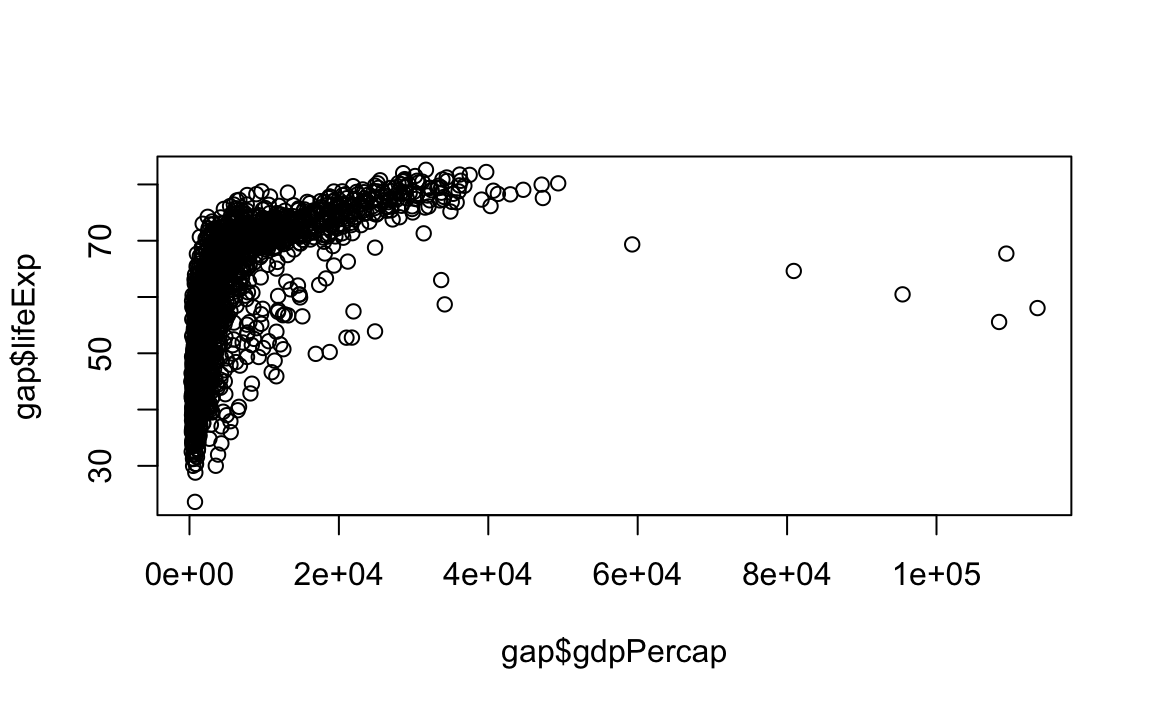
\includegraphics[width=0.7\linewidth]{plsc31101_files/figure-latex/unnamed-chunk-176-1} \end{center}

\subsection{Scatter and Line Plots}\label{scatter-and-line-plots}

The \texttt{type} argument accepts the following character indicators:

\begin{itemize}
\tightlist
\item
  \texttt{"p"}: Point/scatter plots (default plotting behavior).
\end{itemize}

\begin{Shaded}
\begin{Highlighting}[]
\KeywordTok{plot}\NormalTok{(}\DataTypeTok{x =}\NormalTok{ gap}\OperatorTok{$}\NormalTok{gdpPercap, }\DataTypeTok{y =}\NormalTok{ gap}\OperatorTok{$}\NormalTok{lifeExp, }\DataTypeTok{type=}\StringTok{"p"}\NormalTok{)}
\end{Highlighting}
\end{Shaded}

\begin{figure}

{\centering 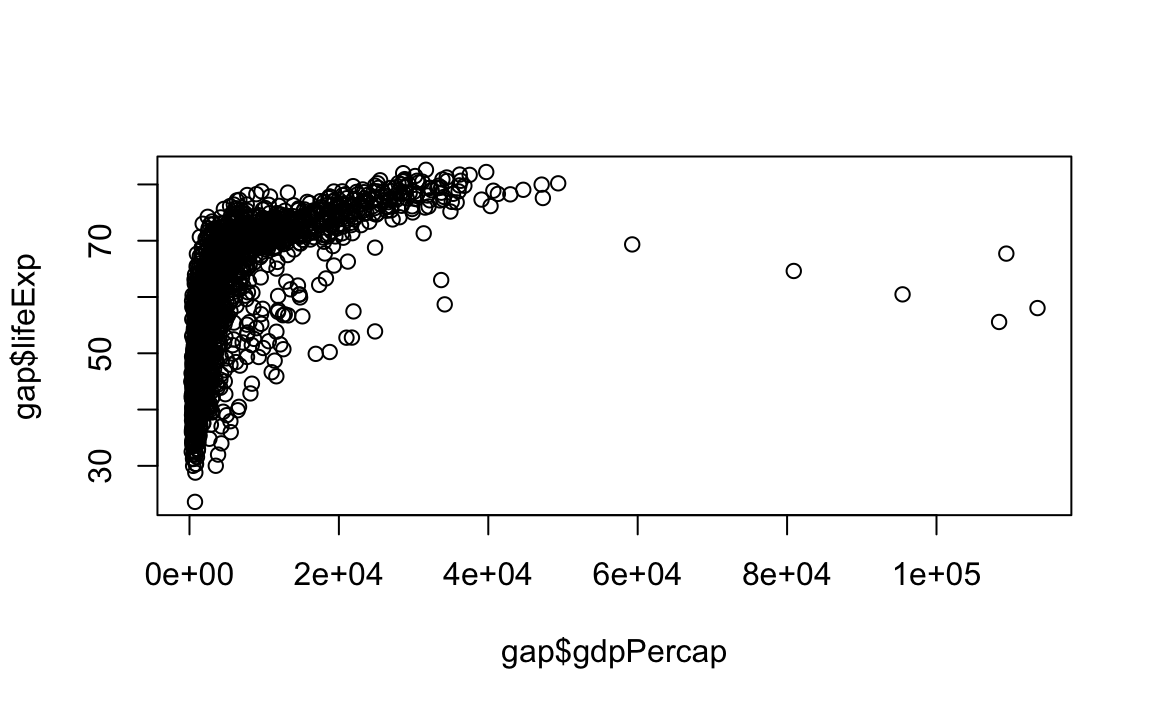
\includegraphics[width=0.7\linewidth]{plsc31101_files/figure-latex/unnamed-chunk-177-1} 

}

\caption{ }\label{fig:unnamed-chunk-177}
\end{figure}

\begin{itemize}
\tightlist
\item
  \texttt{"l"}: Line graphs.
\end{itemize}

\begin{Shaded}
\begin{Highlighting}[]
\CommentTok{# Note that "line" does not create a smooth line, just connected points}
\KeywordTok{plot}\NormalTok{(}\DataTypeTok{x =}\NormalTok{ gap}\OperatorTok{$}\NormalTok{gdpPercap, }\DataTypeTok{y =}\NormalTok{ gap}\OperatorTok{$}\NormalTok{lifeExp, }\DataTypeTok{type=}\StringTok{"l"}\NormalTok{) }
\end{Highlighting}
\end{Shaded}

\begin{figure}

{\centering 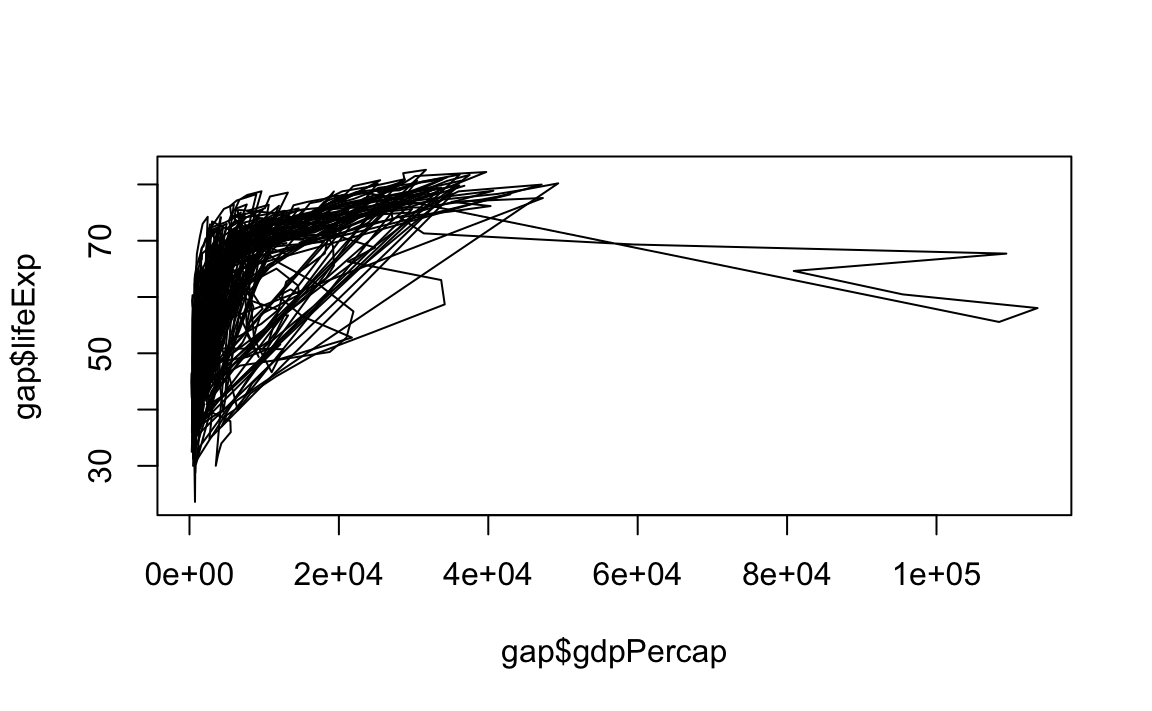
\includegraphics[width=0.7\linewidth]{plsc31101_files/figure-latex/unnamed-chunk-178-1} 

}

\caption{ }\label{fig:unnamed-chunk-178}
\end{figure}

\begin{itemize}
\tightlist
\item
  \texttt{"b"}: Both line and point plots.
\end{itemize}

\begin{Shaded}
\begin{Highlighting}[]
\KeywordTok{plot}\NormalTok{(}\DataTypeTok{x =}\NormalTok{ gap}\OperatorTok{$}\NormalTok{gdpPercap, }\DataTypeTok{y =}\NormalTok{ gap}\OperatorTok{$}\NormalTok{lifeExp, }\DataTypeTok{type=}\StringTok{"b"}\NormalTok{) }
\end{Highlighting}
\end{Shaded}

\begin{figure}

{\centering 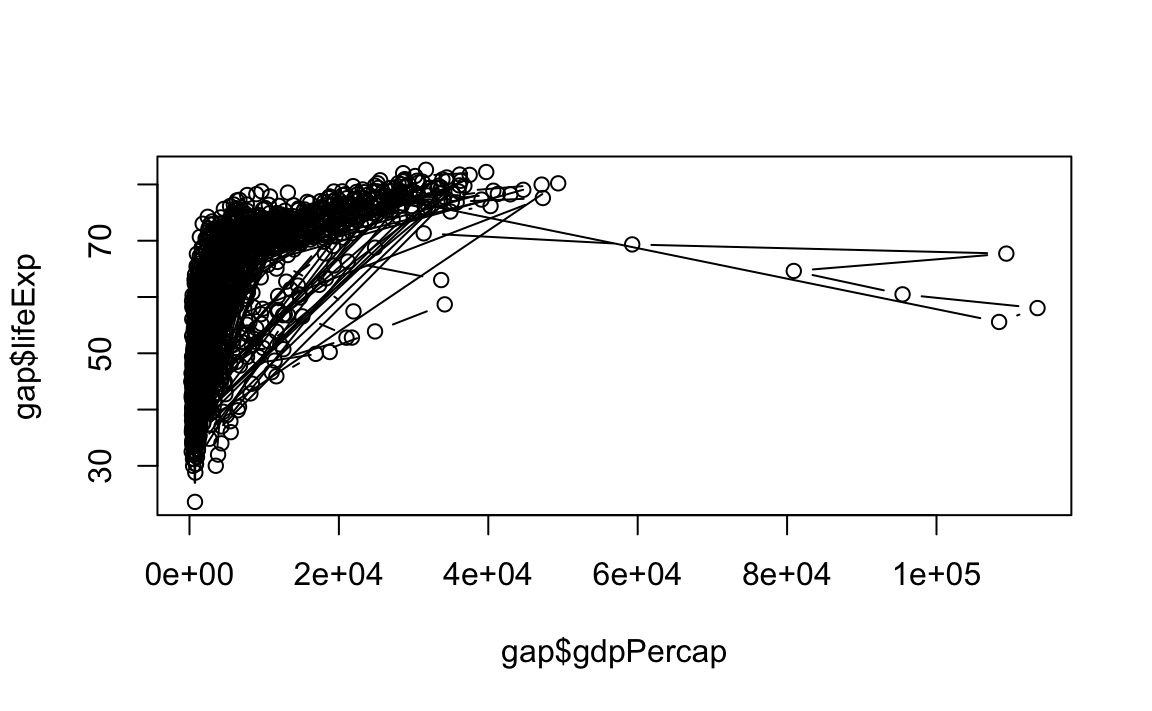
\includegraphics[width=0.7\linewidth]{plsc31101_files/figure-latex/unnamed-chunk-179-1} 

}

\caption{ }\label{fig:unnamed-chunk-179}
\end{figure}

\subsection{Histograms and Density
Plots}\label{histograms-and-density-plots}

Histograms display the frequency of different values of a variable.

\begin{Shaded}
\begin{Highlighting}[]
\KeywordTok{hist}\NormalTok{(}\DataTypeTok{x=}\NormalTok{gap}\OperatorTok{$}\NormalTok{lifeExp)}
\end{Highlighting}
\end{Shaded}

\begin{center}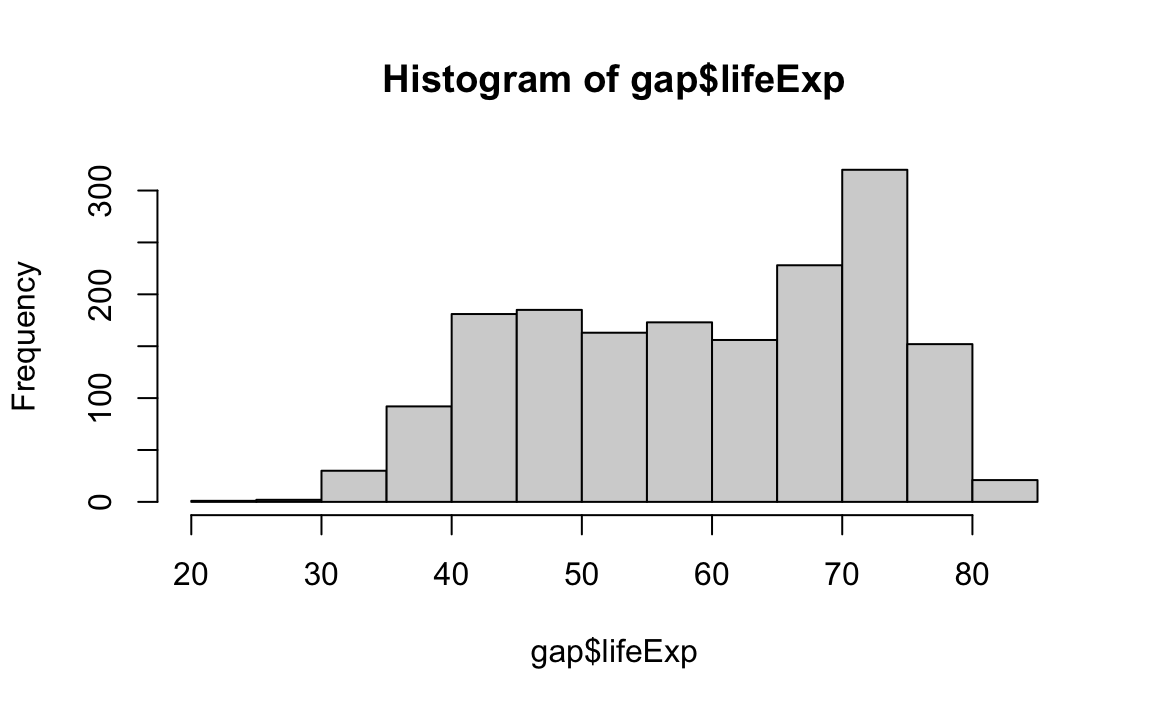
\includegraphics[width=0.7\linewidth]{plsc31101_files/figure-latex/unnamed-chunk-180-1} \end{center}

Histograms require a \texttt{breaks} argument, which determines the
number of bins in the plot. Let's play around with different
\texttt{breaks} values:

\begin{Shaded}
\begin{Highlighting}[]
\KeywordTok{hist}\NormalTok{(}\DataTypeTok{x=}\NormalTok{gap}\OperatorTok{$}\NormalTok{lifeExp, }\DataTypeTok{breaks=}\DecValTok{5}\NormalTok{)}
\KeywordTok{hist}\NormalTok{(}\DataTypeTok{x=}\NormalTok{gap}\OperatorTok{$}\NormalTok{lifeExp, }\DataTypeTok{breaks=}\DecValTok{10}\NormalTok{)}
\end{Highlighting}
\end{Shaded}

\begin{center}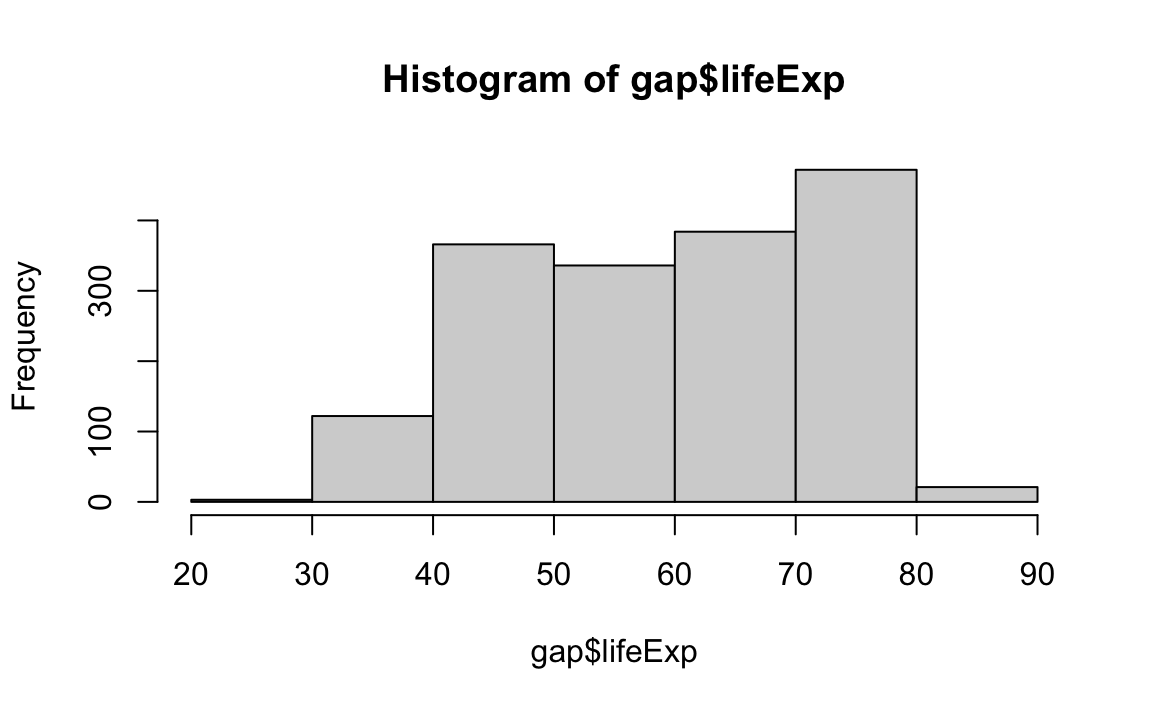
\includegraphics[width=0.7\linewidth]{plsc31101_files/figure-latex/unnamed-chunk-181-1} 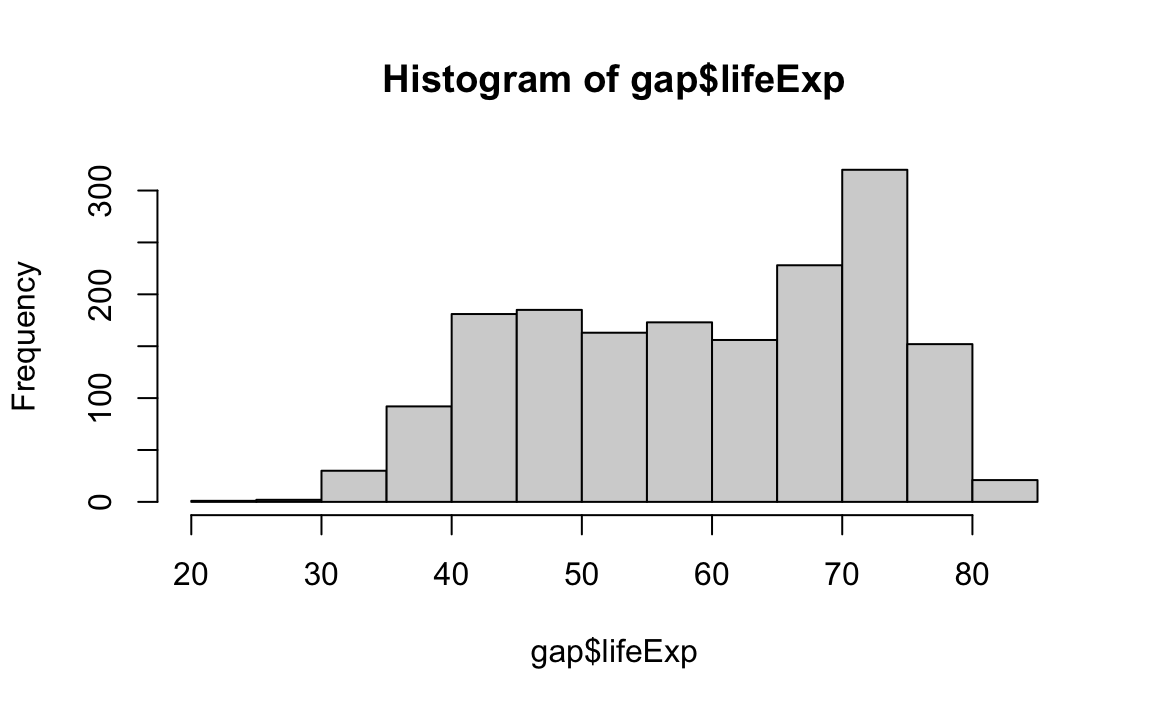
\includegraphics[width=0.7\linewidth]{plsc31101_files/figure-latex/unnamed-chunk-181-2} \end{center}

Density plots are similar; they visualize the distribution of data over
a continuous interval.

\begin{Shaded}
\begin{Highlighting}[]
\CommentTok{# Create a density object (}\AlertTok{NOTE}\CommentTok{: Be sure to remove missing values)}
\NormalTok{age.density <-}\StringTok{ }\KeywordTok{density}\NormalTok{(}\DataTypeTok{x=}\NormalTok{gap}\OperatorTok{$}\NormalTok{lifeExp, }\DataTypeTok{na.rm=}\NormalTok{T)}

\CommentTok{# Plot the density object}
\KeywordTok{plot}\NormalTok{(}\DataTypeTok{x=}\NormalTok{age.density)}
\end{Highlighting}
\end{Shaded}

\begin{figure}

{\centering 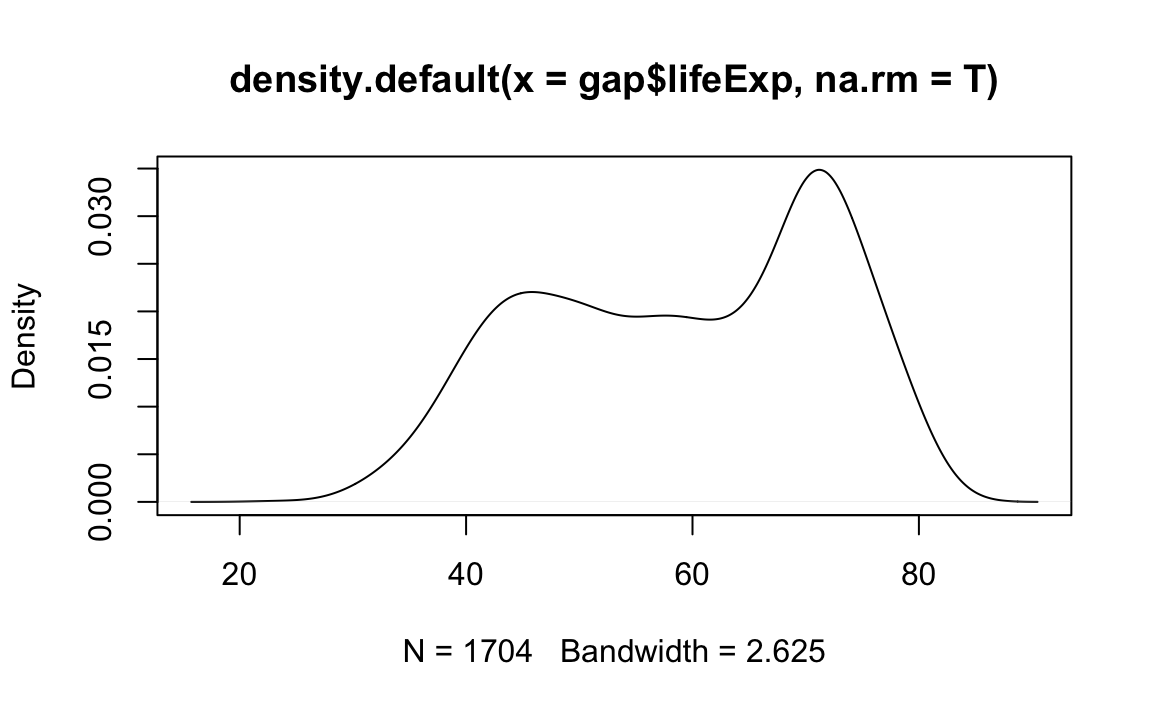
\includegraphics[width=0.7\linewidth]{plsc31101_files/figure-latex/unnamed-chunk-182-1} 

}

\caption{ }\label{fig:unnamed-chunk-182}
\end{figure}

Density passes a \texttt{bw} parameter, which determines the plot's
``bandwidth.''

\begin{Shaded}
\begin{Highlighting}[]
\CommentTok{# Plot the density object, bandwidth of 0.5}
\KeywordTok{plot}\NormalTok{(}\DataTypeTok{x=}\KeywordTok{density}\NormalTok{(}\DataTypeTok{x=}\NormalTok{gap}\OperatorTok{$}\NormalTok{lifeExp, }\DataTypeTok{bw=}\NormalTok{.}\DecValTok{5}\NormalTok{))}
\CommentTok{# Plot the density object, bandwidth of 2}
\KeywordTok{plot}\NormalTok{(}\DataTypeTok{x=}\KeywordTok{density}\NormalTok{(}\DataTypeTok{x=}\NormalTok{gap}\OperatorTok{$}\NormalTok{lifeExp, }\DataTypeTok{bw=}\DecValTok{2}\NormalTok{))}
\CommentTok{# Plot the density object, bandwidth of 6}
\KeywordTok{plot}\NormalTok{(}\DataTypeTok{x=}\KeywordTok{density}\NormalTok{(}\DataTypeTok{x=}\NormalTok{gap}\OperatorTok{$}\NormalTok{lifeExp, }\DataTypeTok{bw=}\DecValTok{6}\NormalTok{)) }
\end{Highlighting}
\end{Shaded}

\begin{center}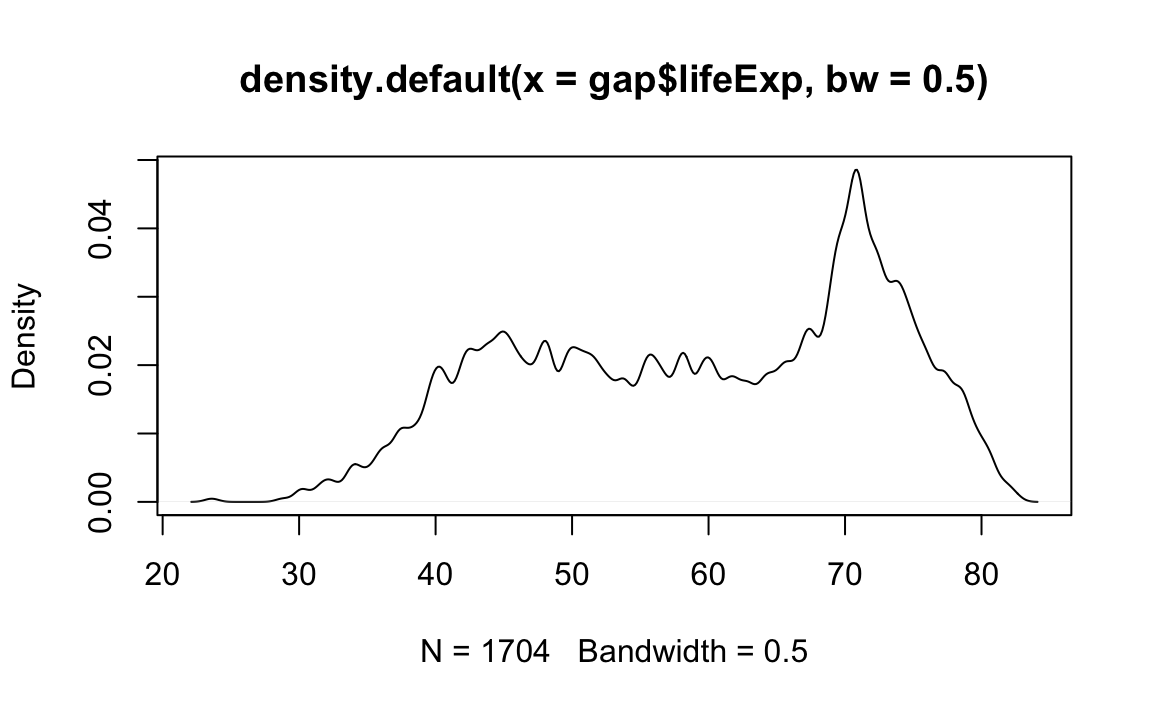
\includegraphics[width=0.7\linewidth]{plsc31101_files/figure-latex/unnamed-chunk-183-1} 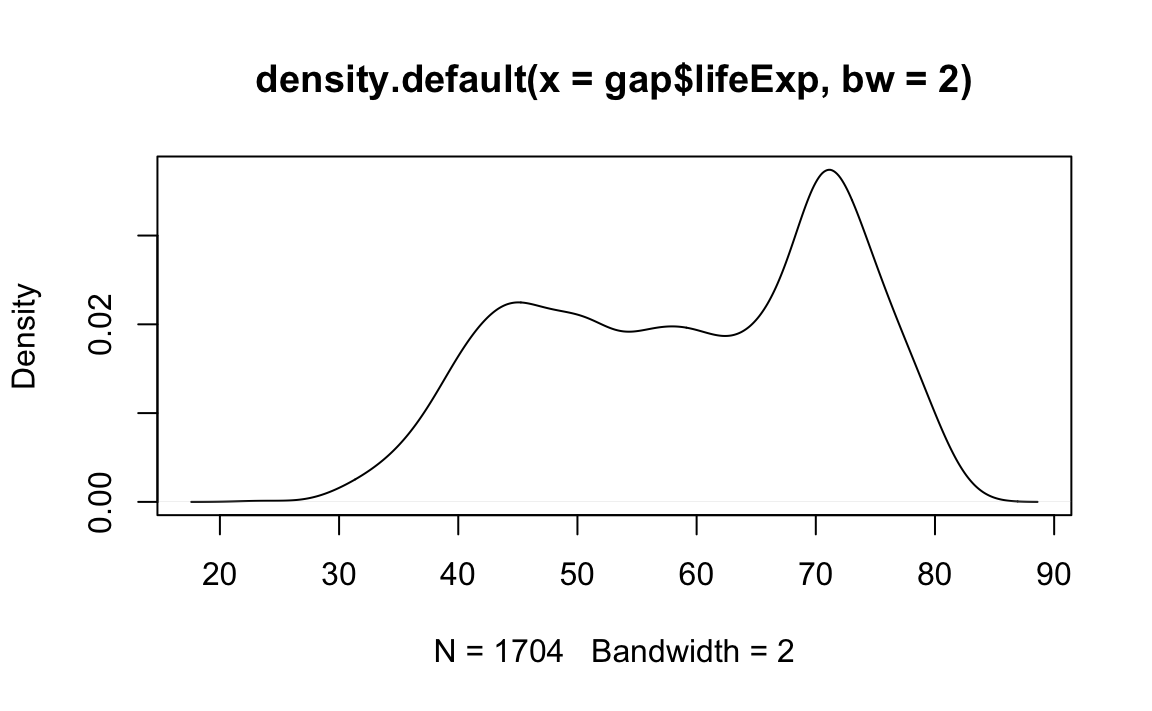
\includegraphics[width=0.7\linewidth]{plsc31101_files/figure-latex/unnamed-chunk-183-2} 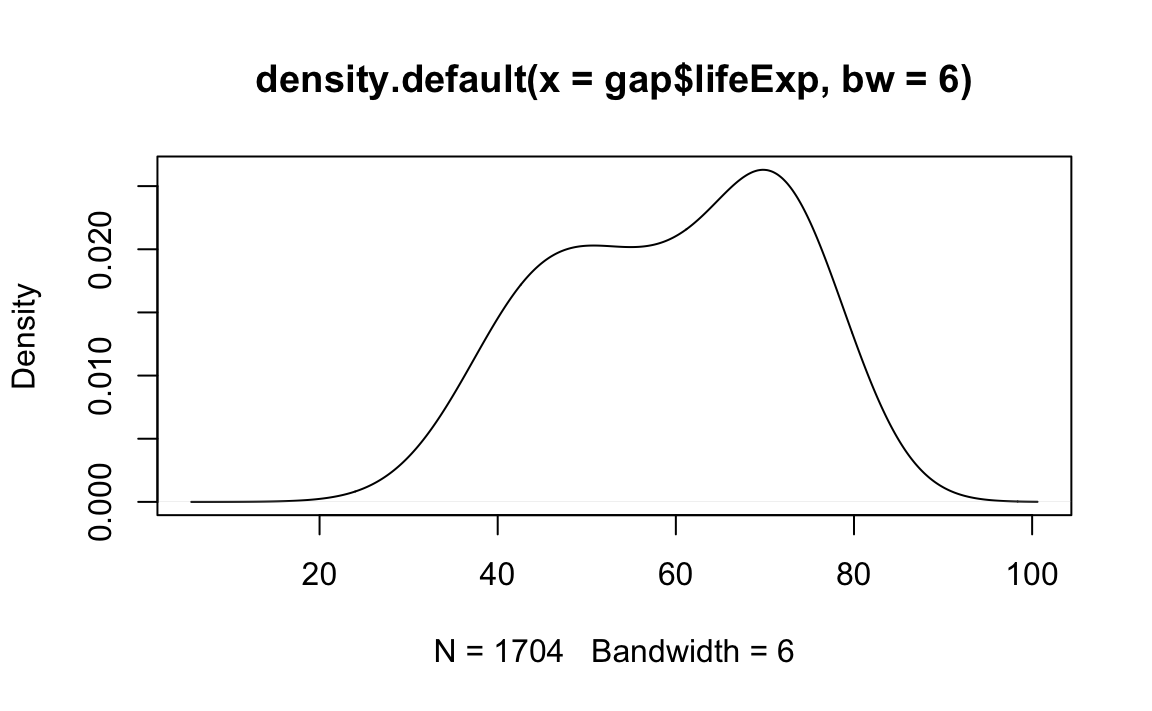
\includegraphics[width=0.7\linewidth]{plsc31101_files/figure-latex/unnamed-chunk-183-3} \end{center}

\subsection{Labels}\label{labels}

Here is the basic call with popular labeling arguments:

\begin{Shaded}
\begin{Highlighting}[]
\KeywordTok{plot}\NormalTok{(}\DataTypeTok{x=}\NormalTok{, }\DataTypeTok{y=}\NormalTok{, }\DataTypeTok{type=}\StringTok{""}\NormalTok{, }\DataTypeTok{xlab=}\StringTok{""}\NormalTok{, }\DataTypeTok{ylab=}\StringTok{""}\NormalTok{, }\DataTypeTok{main=}\StringTok{""}\NormalTok{) }
\end{Highlighting}
\end{Shaded}

From the previous example\ldots{}

\begin{Shaded}
\begin{Highlighting}[]
\KeywordTok{plot}\NormalTok{(}\DataTypeTok{x =}\NormalTok{ gap}\OperatorTok{$}\NormalTok{gdpPercap, }\DataTypeTok{y =}\NormalTok{ gap}\OperatorTok{$}\NormalTok{lifeExp, }\DataTypeTok{type=}\StringTok{"p"}\NormalTok{, }\DataTypeTok{xlab=}\StringTok{"GDP per cap"}\NormalTok{, }\DataTypeTok{ylab=}\StringTok{"Life Expectancy"}\NormalTok{, }\DataTypeTok{main=}\StringTok{"Life Expectancy ~ GDP"}\NormalTok{) }\CommentTok{# Add labels for axes and overall plot}
\end{Highlighting}
\end{Shaded}

\begin{figure}

{\centering 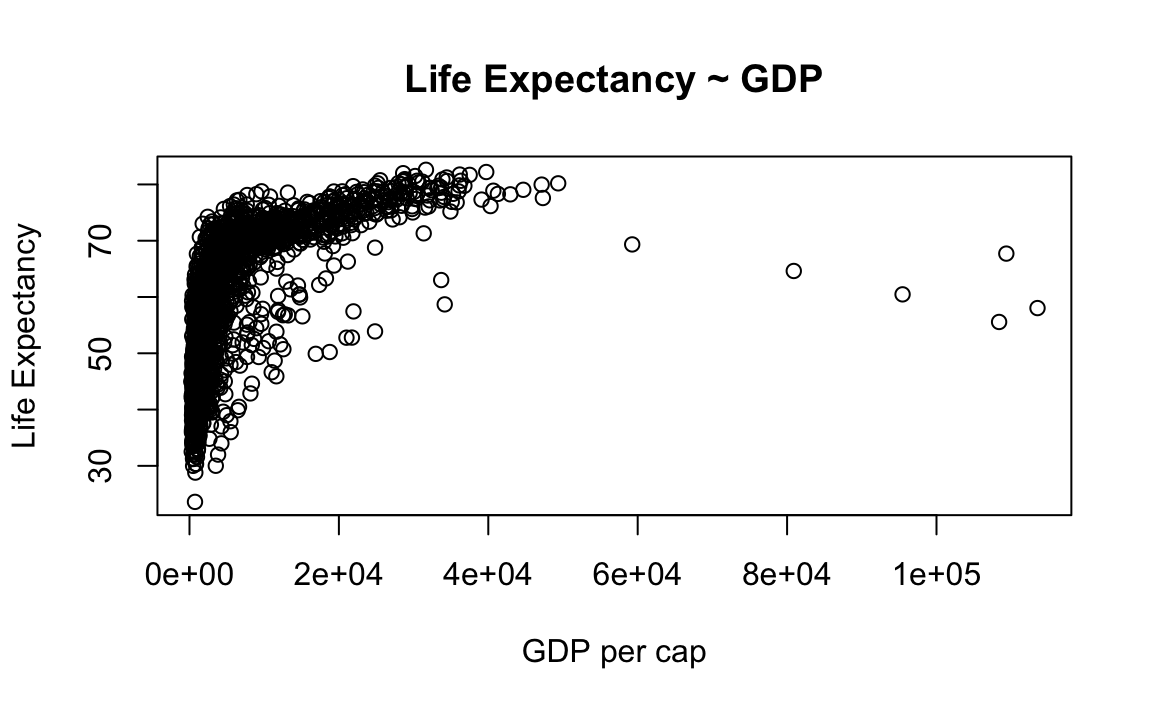
\includegraphics[width=0.7\linewidth]{plsc31101_files/figure-latex/unnamed-chunk-185-1} 

}

\caption{ }\label{fig:unnamed-chunk-185}
\end{figure}

\subsection{Axis and Size Scaling}\label{axis-and-size-scaling}

Currently it is hard to see the relationship between the points due to
some strong outliers in GDP per capita. We can change the scale of units
on the x-axis using scaling arguments.

Here is the basic call with popular scaling arguments:

\begin{Shaded}
\begin{Highlighting}[]
\KeywordTok{plot}\NormalTok{(}\DataTypeTok{x=}\NormalTok{, }\DataTypeTok{y=}\NormalTok{, }\DataTypeTok{type=}\StringTok{""}\NormalTok{, }\DataTypeTok{xlim=}\NormalTok{, }\DataTypeTok{ylim=}\NormalTok{, }\DataTypeTok{cex=}\NormalTok{)}
\end{Highlighting}
\end{Shaded}

From the previous example\ldots{}

\begin{Shaded}
\begin{Highlighting}[]
\CommentTok{# Create a basic plot}
\KeywordTok{plot}\NormalTok{(}\DataTypeTok{x =}\NormalTok{ gap}\OperatorTok{$}\NormalTok{gdpPercap, }\DataTypeTok{y =}\NormalTok{ gap}\OperatorTok{$}\NormalTok{lifeExp, }\DataTypeTok{type=}\StringTok{"p"}\NormalTok{)}
\CommentTok{# Limit gdp (x-axis) to between 1,000 and 20,000}
\KeywordTok{plot}\NormalTok{(}\DataTypeTok{x =}\NormalTok{ gap}\OperatorTok{$}\NormalTok{gdpPercap, }\DataTypeTok{y =}\NormalTok{ gap}\OperatorTok{$}\NormalTok{lifeExp, }\DataTypeTok{xlim =} \KeywordTok{c}\NormalTok{(}\DecValTok{1000}\NormalTok{,}\DecValTok{20000}\NormalTok{)) }
\CommentTok{# Limit gdp (x-axis) to between 1,000 and 20,000, increase point size to 2}
\KeywordTok{plot}\NormalTok{(}\DataTypeTok{x =}\NormalTok{ gap}\OperatorTok{$}\NormalTok{gdpPercap, }\DataTypeTok{y =}\NormalTok{ gap}\OperatorTok{$}\NormalTok{lifeExp, }\DataTypeTok{xlim =} \KeywordTok{c}\NormalTok{(}\DecValTok{1000}\NormalTok{,}\DecValTok{20000}\NormalTok{), }\DataTypeTok{cex=}\DecValTok{2}\NormalTok{) }
\CommentTok{# Limit gdp (x-axis) to between 1,000 and 20,000, decrease point size to 0.5}
\KeywordTok{plot}\NormalTok{(}\DataTypeTok{x =}\NormalTok{ gap}\OperatorTok{$}\NormalTok{gdpPercap, }\DataTypeTok{y =}\NormalTok{ gap}\OperatorTok{$}\NormalTok{lifeExp, }\DataTypeTok{xlim =} \KeywordTok{c}\NormalTok{(}\DecValTok{1000}\NormalTok{,}\DecValTok{20000}\NormalTok{), }\DataTypeTok{cex=}\FloatTok{0.5}\NormalTok{)  }
\end{Highlighting}
\end{Shaded}

\begin{figure}

{\centering 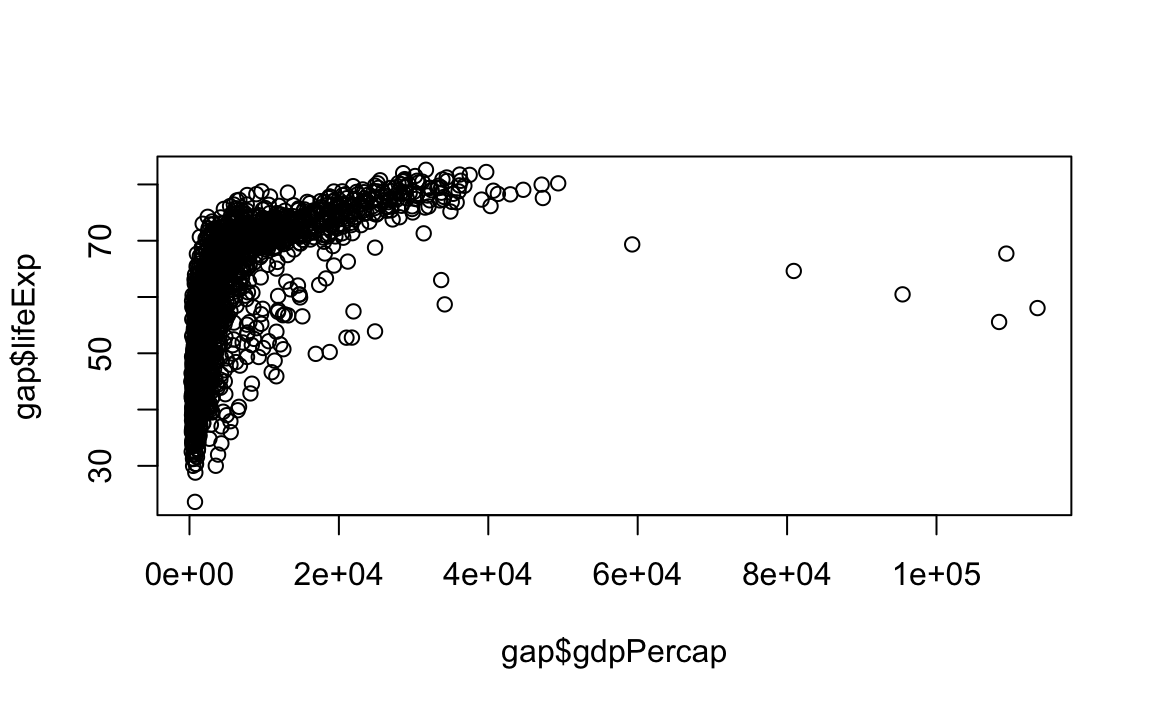
\includegraphics[width=0.7\linewidth]{plsc31101_files/figure-latex/unnamed-chunk-187-1} 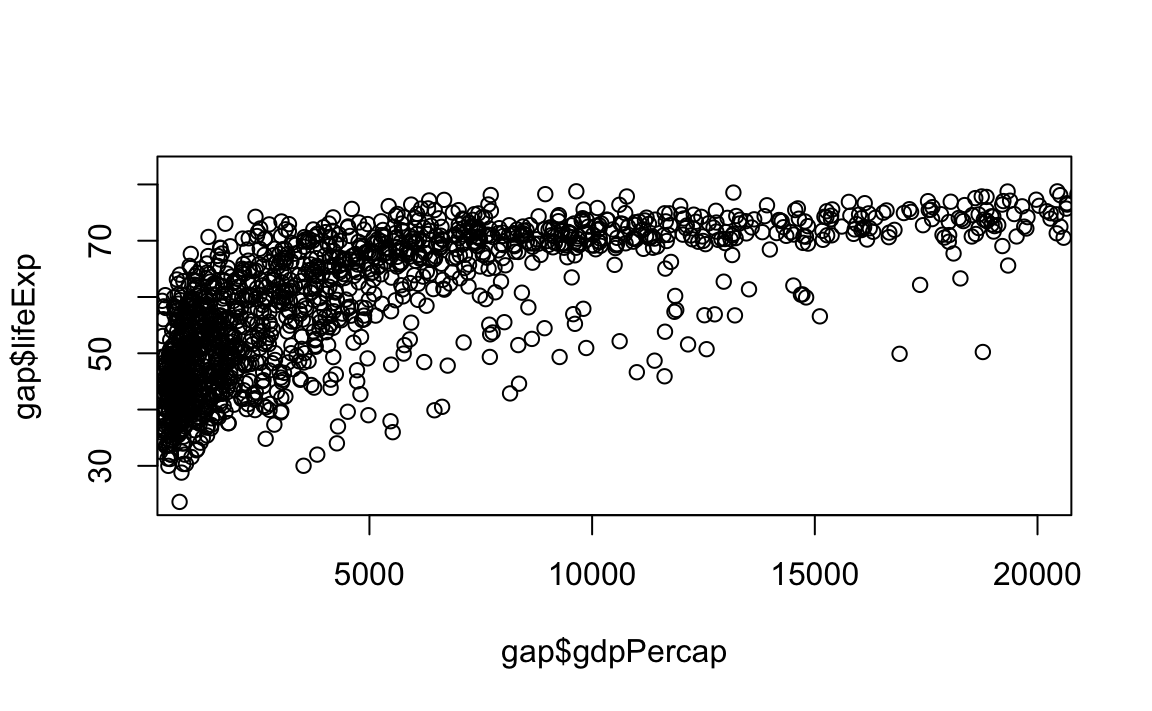
\includegraphics[width=0.7\linewidth]{plsc31101_files/figure-latex/unnamed-chunk-187-2} 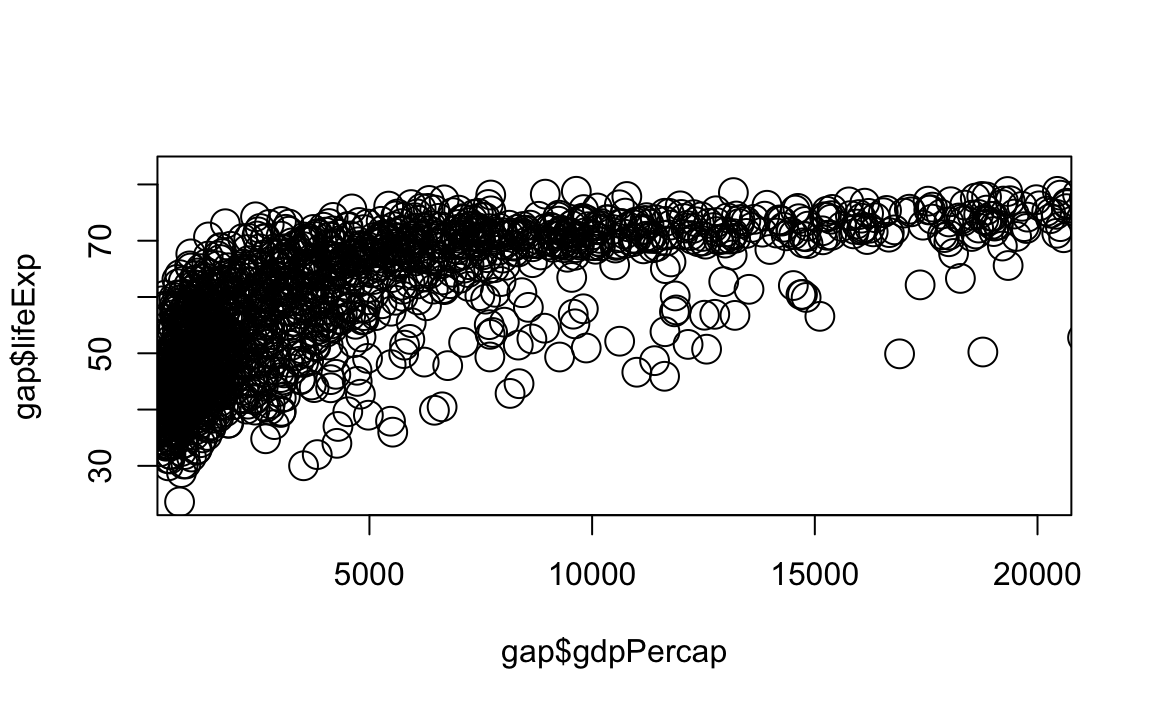
\includegraphics[width=0.7\linewidth]{plsc31101_files/figure-latex/unnamed-chunk-187-3} 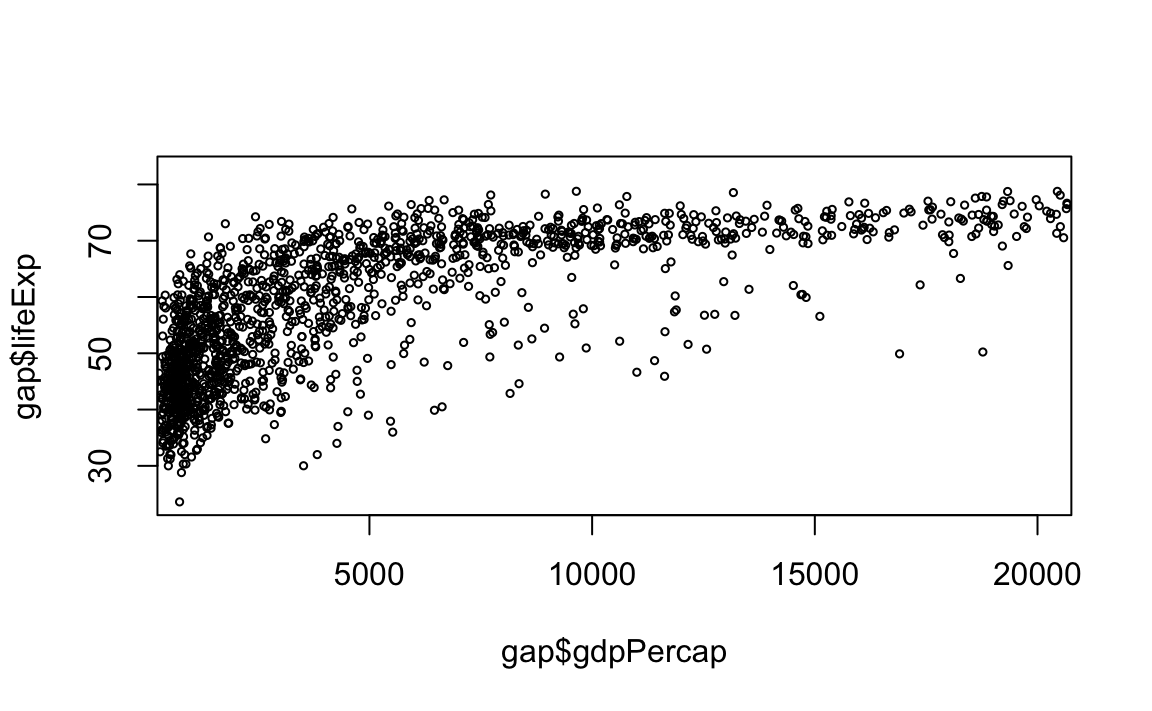
\includegraphics[width=0.7\linewidth]{plsc31101_files/figure-latex/unnamed-chunk-187-4} 

}

\caption{ }\label{fig:unnamed-chunk-187}
\end{figure}

\subsection{Graphical Parameters}\label{graphical-parameters}

We can change the points with a number of graphical options:

\begin{Shaded}
\begin{Highlighting}[]
\KeywordTok{plot}\NormalTok{(}\DataTypeTok{x=}\NormalTok{, }\DataTypeTok{y=}\NormalTok{, }\DataTypeTok{type=}\StringTok{""}\NormalTok{, }\DataTypeTok{col=}\StringTok{""}\NormalTok{, }\DataTypeTok{pch=}\NormalTok{, }\DataTypeTok{lty=}\NormalTok{, }\DataTypeTok{lwd=}\NormalTok{)}
\end{Highlighting}
\end{Shaded}

\begin{itemize}
\tightlist
\item
  Colors
\end{itemize}

\begin{Shaded}
\begin{Highlighting}[]
\KeywordTok{library}\NormalTok{(dplyr)}
\KeywordTok{colors}\NormalTok{() }\OperatorTok
\StringTok{  }\KeywordTok{head}\NormalTok{(}\DecValTok{20}\NormalTok{)}\CommentTok{# View first 20 elements of the color vector}
\CommentTok{#>  [1] "white"         "aliceblue"     "antiquewhite"  "antiquewhite1"}
\CommentTok{#>  [5] "antiquewhite2" "antiquewhite3" "antiquewhite4" "aquamarine"   }
\CommentTok{#>  [9] "aquamarine1"   "aquamarine2"   "aquamarine3"   "aquamarine4"  }
\CommentTok{#> [13] "azure"         "azure1"        "azure2"        "azure3"       }
\CommentTok{#> [17] "azure4"        "beige"         "bisque"        "bisque1"}
\end{Highlighting}
\end{Shaded}

Another option:
\href{http://research.stowers-institute.org/efg/R/Color/Chart/ColorsChart1.jpg}{R
Color Infographic}

\begin{Shaded}
\begin{Highlighting}[]
\KeywordTok{plot}\NormalTok{(}\DataTypeTok{x =}\NormalTok{ gap}\OperatorTok{$}\NormalTok{gdpPercap, }\DataTypeTok{y =}\NormalTok{ gap}\OperatorTok{$}\NormalTok{lifeExp, }\DataTypeTok{type=}\StringTok{"p"}\NormalTok{, }\DataTypeTok{col=}\StringTok{"aquamarine1"}\NormalTok{)}
\end{Highlighting}
\end{Shaded}

\begin{figure}

{\centering 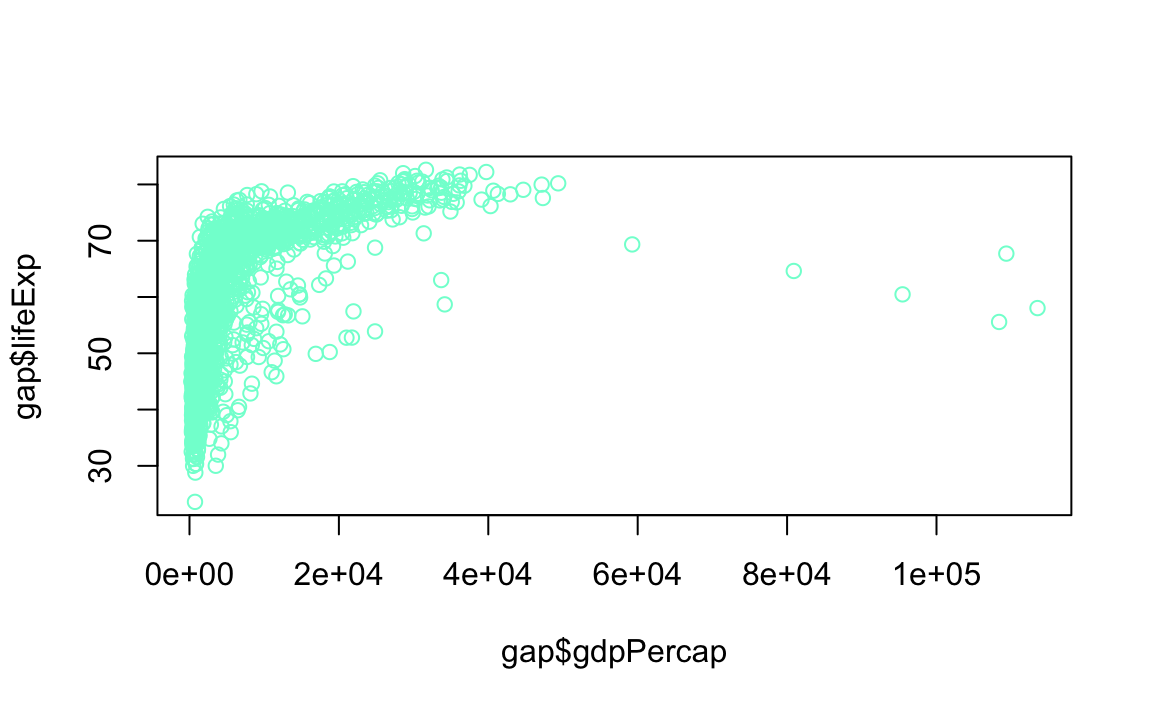
\includegraphics[width=0.7\linewidth]{plsc31101_files/figure-latex/unnamed-chunk-190-1} 

}

\caption{ }\label{fig:unnamed-chunk-190}
\end{figure}

\begin{itemize}
\tightlist
\item
  Point Styles and Widths
\end{itemize}

\href{http://www.endmemo.com/program/R/pic/pchsymbols.png}{A Good
Reference}

\begin{Shaded}
\begin{Highlighting}[]
\CommentTok{# Change point style to crosses}
\KeywordTok{plot}\NormalTok{(}\DataTypeTok{x =}\NormalTok{ gap}\OperatorTok{$}\NormalTok{gdpPercap, }\DataTypeTok{y =}\NormalTok{ gap}\OperatorTok{$}\NormalTok{lifeExp, }\DataTypeTok{type=}\StringTok{"p"}\NormalTok{, }\DataTypeTok{pch=}\DecValTok{3}\NormalTok{) }
\CommentTok{# Change point style to filled squares}
\KeywordTok{plot}\NormalTok{(}\DataTypeTok{x =}\NormalTok{ gap}\OperatorTok{$}\NormalTok{gdpPercap, }\DataTypeTok{y =}\NormalTok{ gap}\OperatorTok{$}\NormalTok{lifeExp, }\DataTypeTok{type=}\StringTok{"p"}\NormalTok{, }\DataTypeTok{pch=}\DecValTok{15}\NormalTok{) }
\CommentTok{# Change point style to filled squares and increase point size to 3}
\KeywordTok{plot}\NormalTok{(}\DataTypeTok{x =}\NormalTok{ gap}\OperatorTok{$}\NormalTok{gdpPercap, }\DataTypeTok{y =}\NormalTok{ gap}\OperatorTok{$}\NormalTok{lifeExp, }\DataTypeTok{type=}\StringTok{"p"}\NormalTok{, }\DataTypeTok{pch=}\DecValTok{15}\NormalTok{, }\DataTypeTok{cex=}\DecValTok{3}\NormalTok{) }
\CommentTok{# Change point style to "w"}
\KeywordTok{plot}\NormalTok{(}\DataTypeTok{x =}\NormalTok{ gap}\OperatorTok{$}\NormalTok{gdpPercap, }\DataTypeTok{y =}\NormalTok{ gap}\OperatorTok{$}\NormalTok{lifeExp, }\DataTypeTok{type=}\StringTok{"p"}\NormalTok{, }\DataTypeTok{pch=}\StringTok{"w"}\NormalTok{)}
\CommentTok{# Change point style to "$" and increase point size to 2}
\KeywordTok{plot}\NormalTok{(}\DataTypeTok{x =}\NormalTok{ gap}\OperatorTok{$}\NormalTok{gdpPercap, }\DataTypeTok{y =}\NormalTok{ gap}\OperatorTok{$}\NormalTok{lifeExp, }\DataTypeTok{type=}\StringTok{"p"}\NormalTok{, }\DataTypeTok{pch=}\StringTok{"$"}\NormalTok{, }\DataTypeTok{cex=}\DecValTok{2}\NormalTok{) }
\end{Highlighting}
\end{Shaded}

\begin{figure}

{\centering 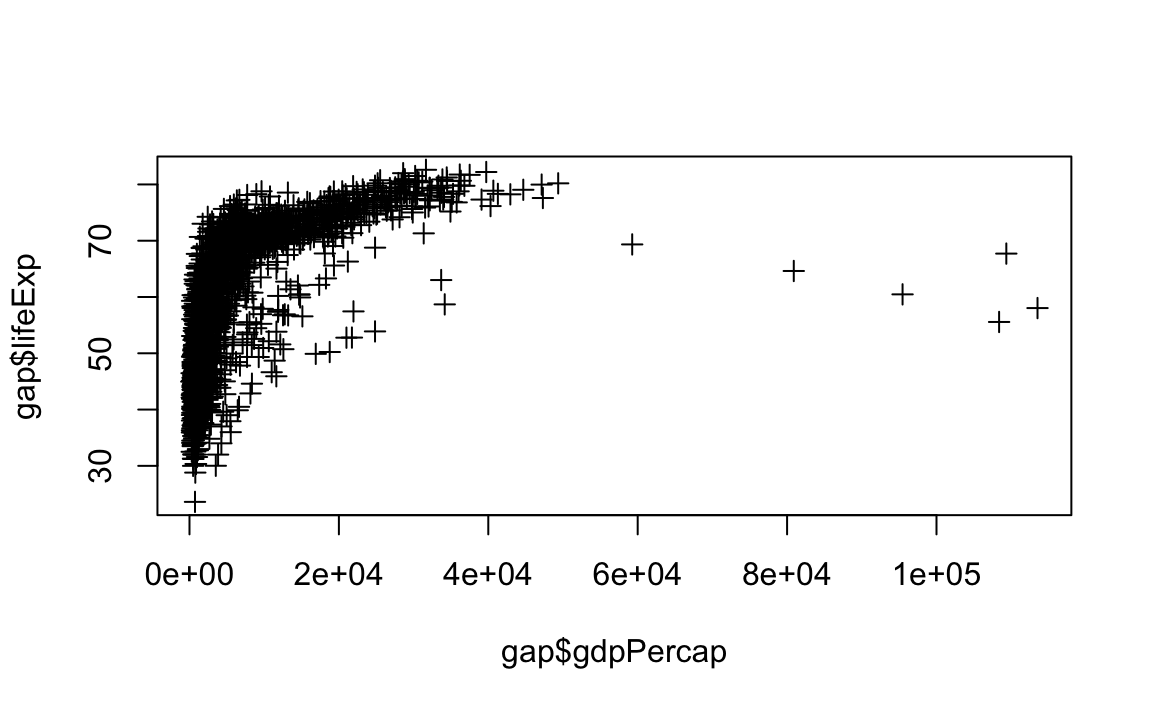
\includegraphics[width=0.7\linewidth]{plsc31101_files/figure-latex/unnamed-chunk-191-1} 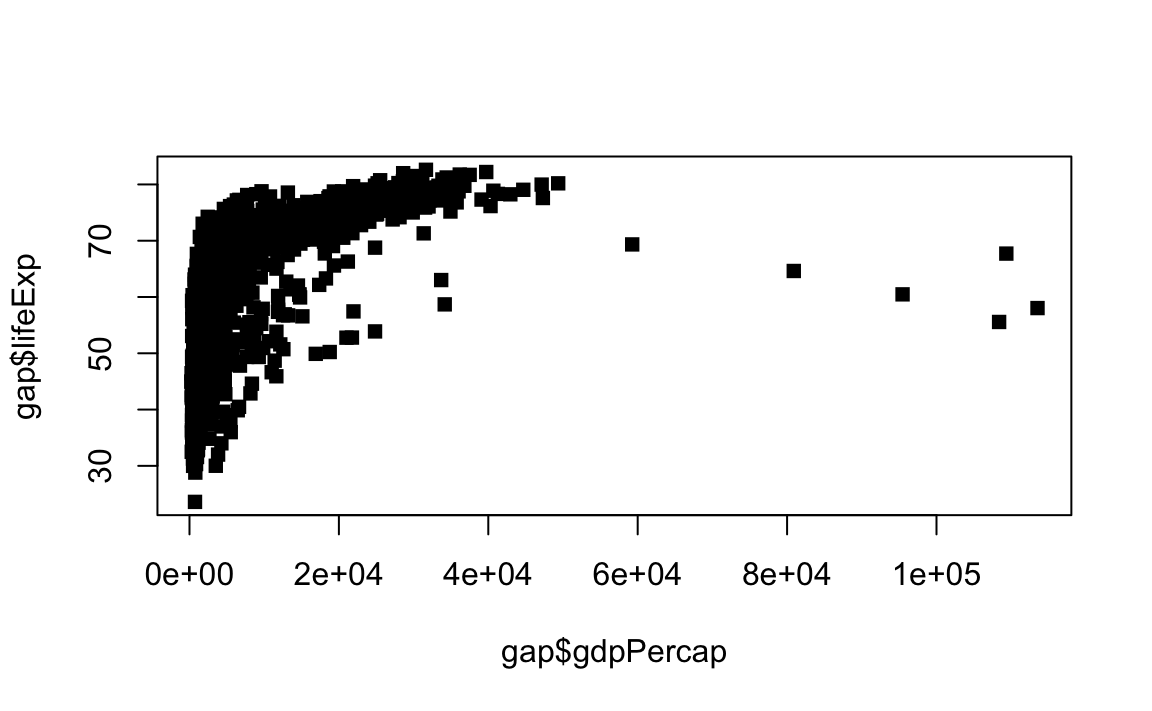
\includegraphics[width=0.7\linewidth]{plsc31101_files/figure-latex/unnamed-chunk-191-2} 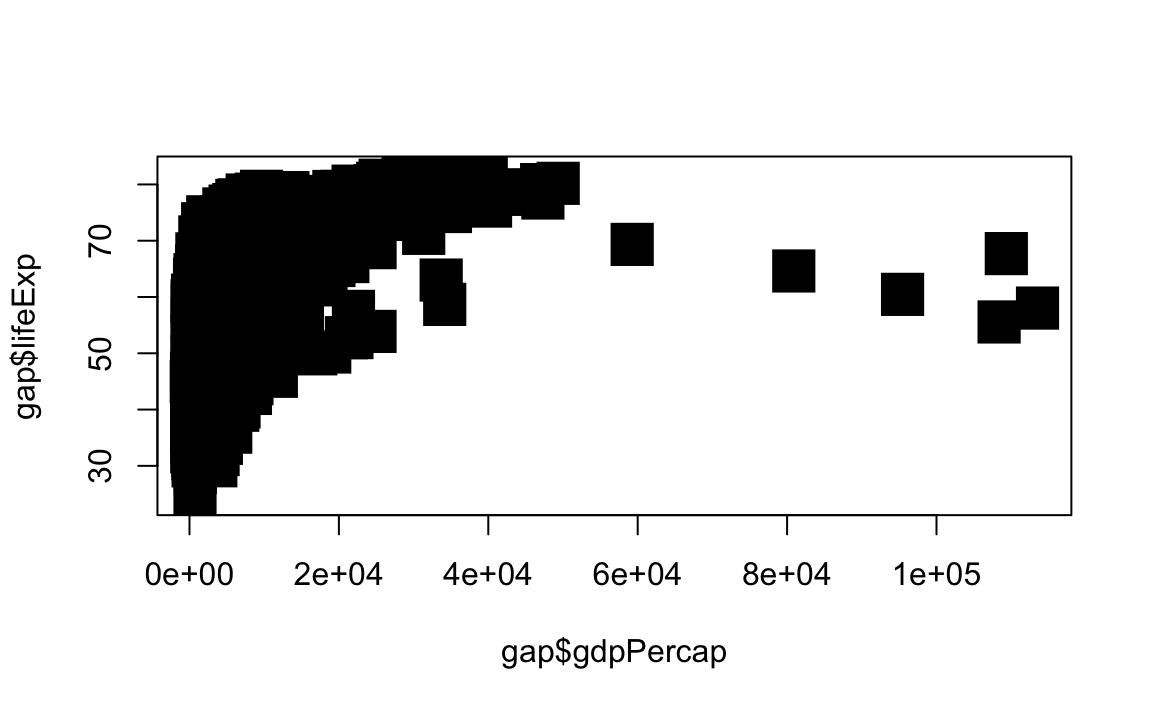
\includegraphics[width=0.7\linewidth]{plsc31101_files/figure-latex/unnamed-chunk-191-3} 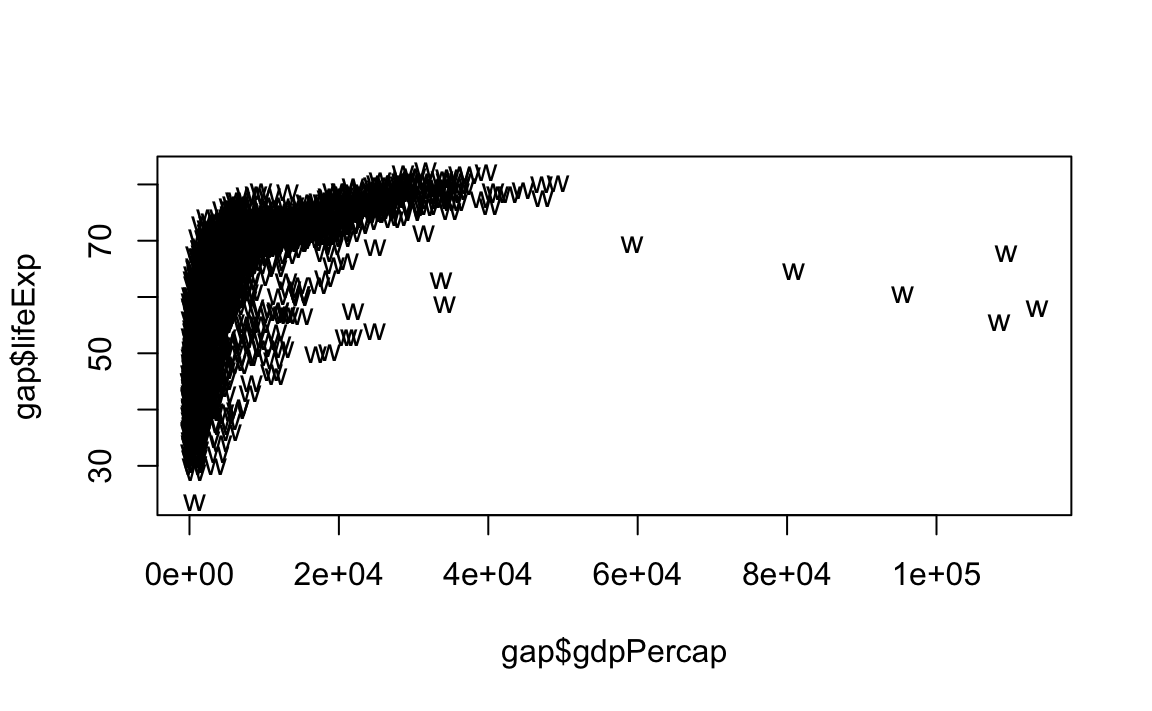
\includegraphics[width=0.7\linewidth]{plsc31101_files/figure-latex/unnamed-chunk-191-4} 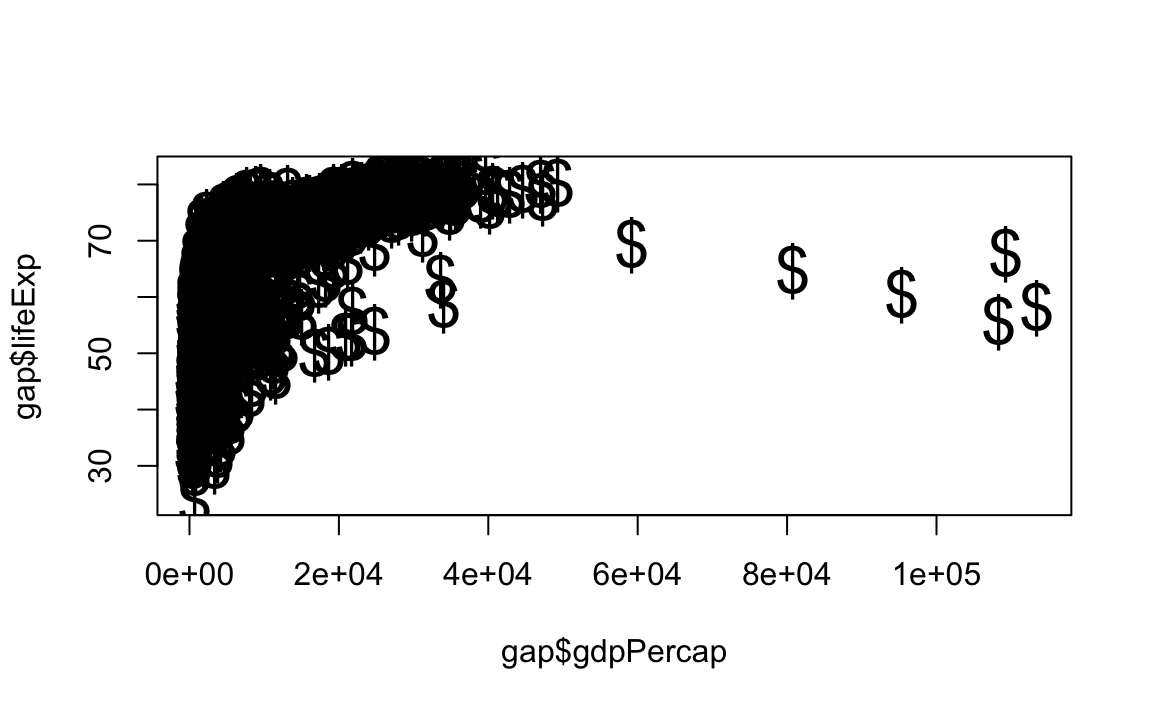
\includegraphics[width=0.7\linewidth]{plsc31101_files/figure-latex/unnamed-chunk-191-5} 

}

\caption{ }\label{fig:unnamed-chunk-191}
\end{figure}

\begin{itemize}
\tightlist
\item
  Line Styles and Widths
\end{itemize}

\begin{Shaded}
\begin{Highlighting}[]
\CommentTok{# Line plot with solid line}
\KeywordTok{plot}\NormalTok{(}\DataTypeTok{x =}\NormalTok{ gap}\OperatorTok{$}\NormalTok{gdpPercap, }\DataTypeTok{y =}\NormalTok{ gap}\OperatorTok{$}\NormalTok{lifeExp, }\DataTypeTok{type=}\StringTok{"l"}\NormalTok{, }\DataTypeTok{lty=}\DecValTok{1}\NormalTok{)}
\CommentTok{# Line plot with medium dashed line}
\KeywordTok{plot}\NormalTok{(}\DataTypeTok{x =}\NormalTok{ gap}\OperatorTok{$}\NormalTok{gdpPercap, }\DataTypeTok{y =}\NormalTok{ gap}\OperatorTok{$}\NormalTok{lifeExp, }\DataTypeTok{type=}\StringTok{"l"}\NormalTok{, }\DataTypeTok{lty=}\DecValTok{2}\NormalTok{)}
\CommentTok{# Line plot with short dashed line}
\KeywordTok{plot}\NormalTok{(}\DataTypeTok{x =}\NormalTok{ gap}\OperatorTok{$}\NormalTok{gdpPercap, }\DataTypeTok{y =}\NormalTok{ gap}\OperatorTok{$}\NormalTok{lifeExp, }\DataTypeTok{type=}\StringTok{"l"}\NormalTok{, }\DataTypeTok{lty=}\DecValTok{3}\NormalTok{)}
\CommentTok{# Change line width to 2}
\KeywordTok{plot}\NormalTok{(}\DataTypeTok{x =}\NormalTok{ gap}\OperatorTok{$}\NormalTok{gdpPercap, }\DataTypeTok{y =}\NormalTok{ gap}\OperatorTok{$}\NormalTok{lifeExp, }\DataTypeTok{type=}\StringTok{"l"}\NormalTok{, }\DataTypeTok{lty=}\DecValTok{3}\NormalTok{, }\DataTypeTok{lwd=}\DecValTok{2}\NormalTok{)}
\CommentTok{# Change line width to 5}
\KeywordTok{plot}\NormalTok{(}\DataTypeTok{x =}\NormalTok{ gap}\OperatorTok{$}\NormalTok{gdpPercap, }\DataTypeTok{y =}\NormalTok{ gap}\OperatorTok{$}\NormalTok{lifeExp, }\DataTypeTok{type=}\StringTok{"l"}\NormalTok{,  }\DataTypeTok{lwd=}\DecValTok{5}\NormalTok{)}
\CommentTok{# Change line width to 10 and use dash-dot}
\KeywordTok{plot}\NormalTok{(}\DataTypeTok{x =}\NormalTok{ gap}\OperatorTok{$}\NormalTok{gdpPercap, }\DataTypeTok{y =}\NormalTok{ gap}\OperatorTok{$}\NormalTok{lifeExp, }\DataTypeTok{type=}\StringTok{"l"}\NormalTok{,  }\DataTypeTok{lty=}\DecValTok{4}\NormalTok{, }\DataTypeTok{lwd=}\DecValTok{10}\NormalTok{)}
\end{Highlighting}
\end{Shaded}

\begin{figure}

{\centering 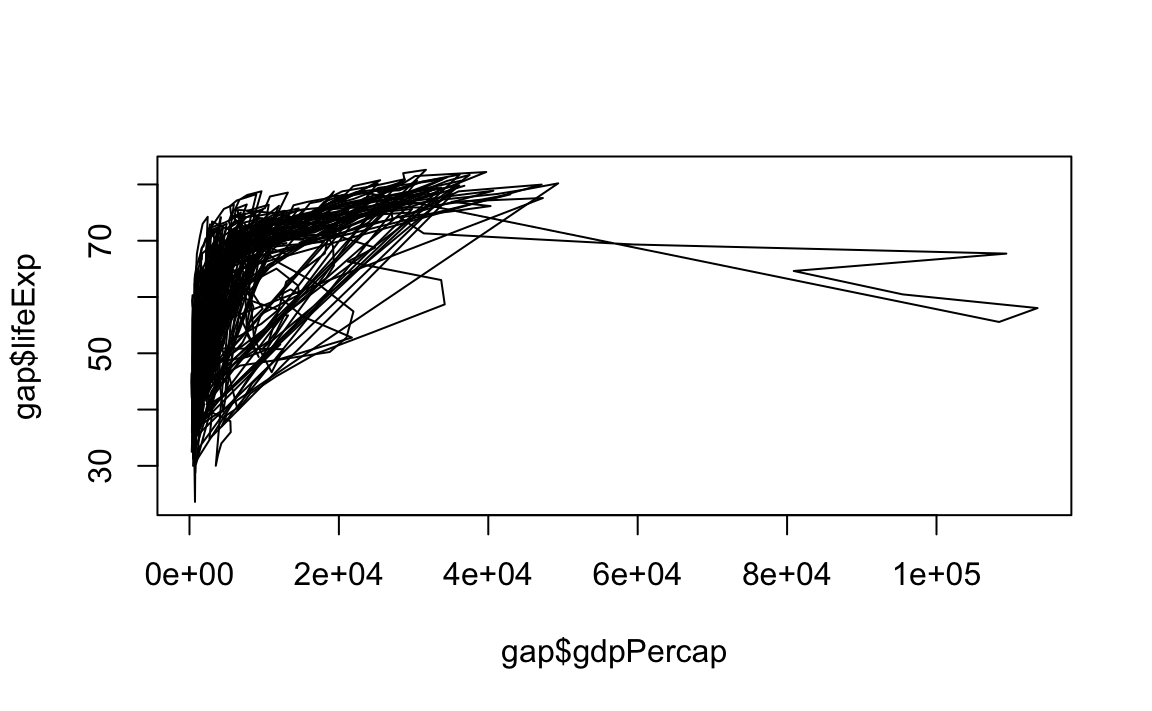
\includegraphics[width=0.7\linewidth]{plsc31101_files/figure-latex/unnamed-chunk-192-1} 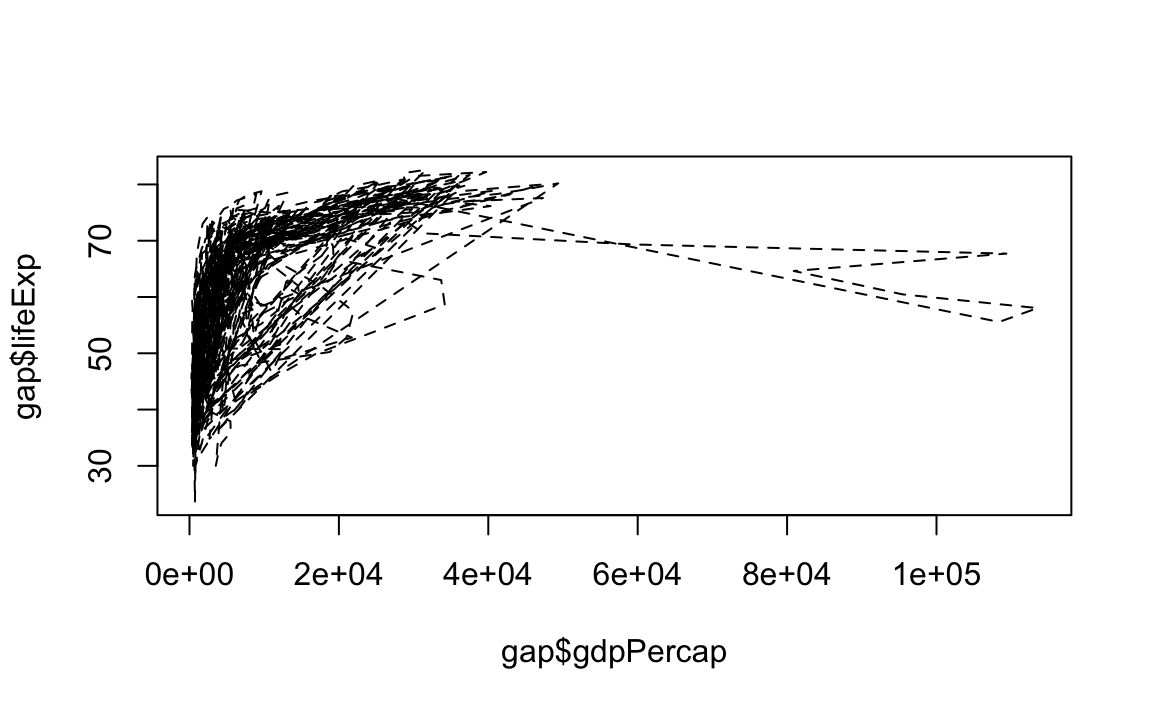
\includegraphics[width=0.7\linewidth]{plsc31101_files/figure-latex/unnamed-chunk-192-2} 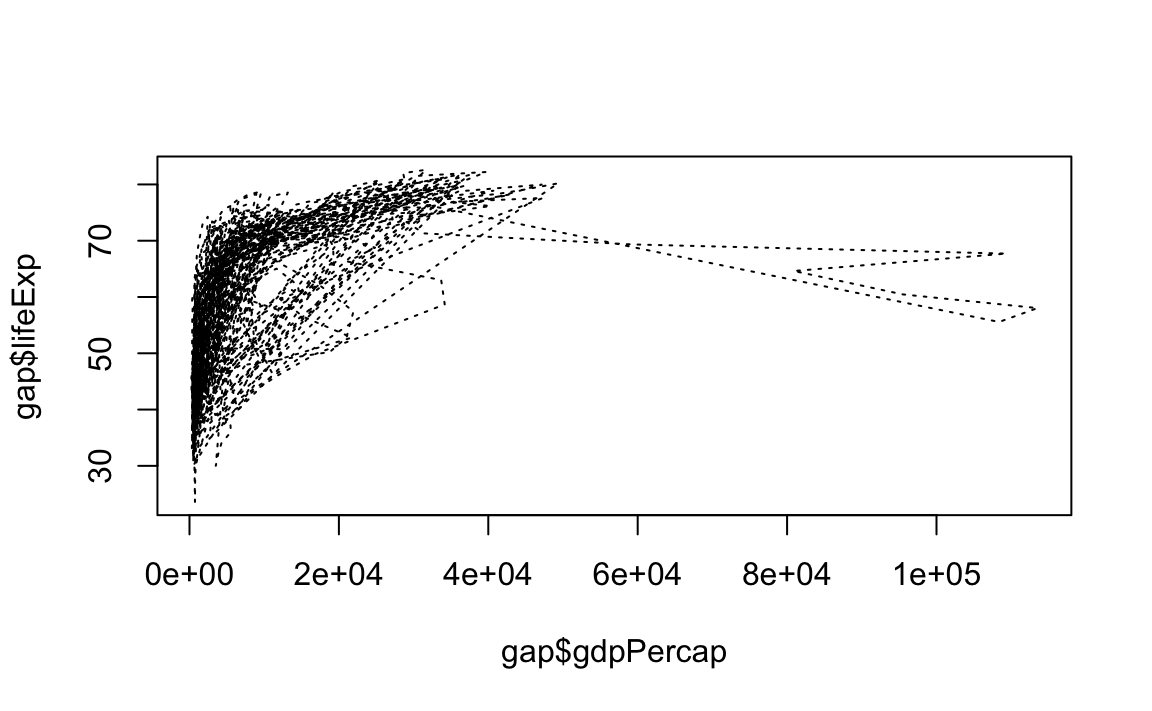
\includegraphics[width=0.7\linewidth]{plsc31101_files/figure-latex/unnamed-chunk-192-3} 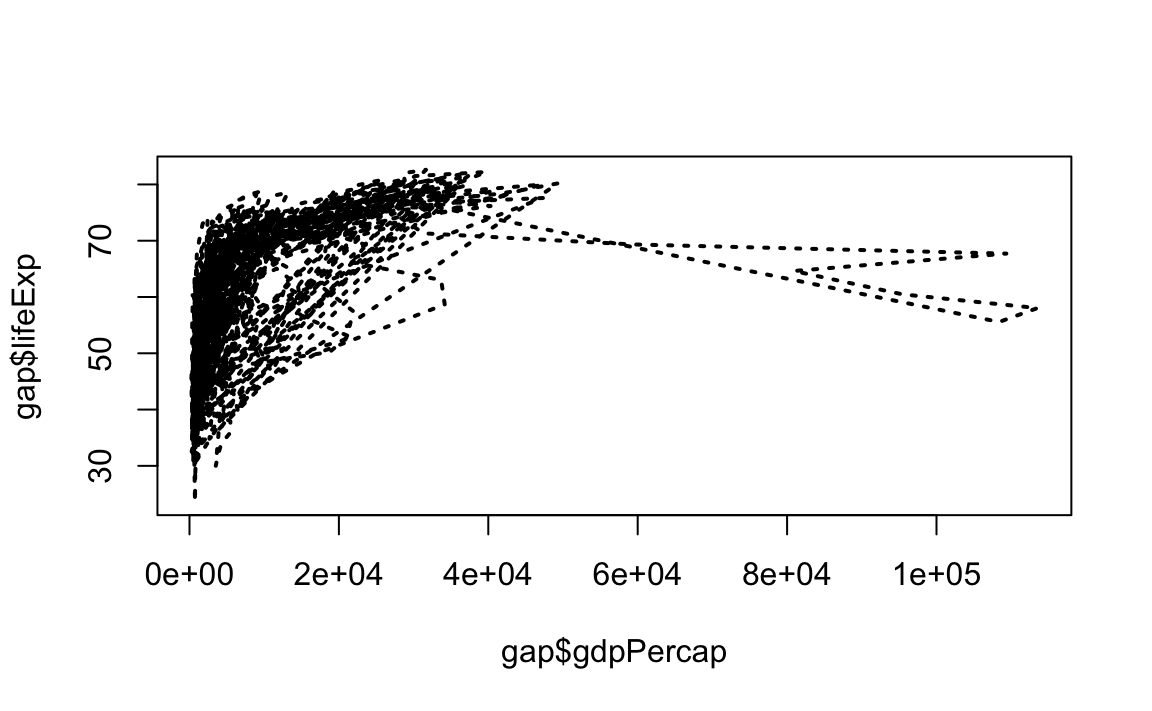
\includegraphics[width=0.7\linewidth]{plsc31101_files/figure-latex/unnamed-chunk-192-4} 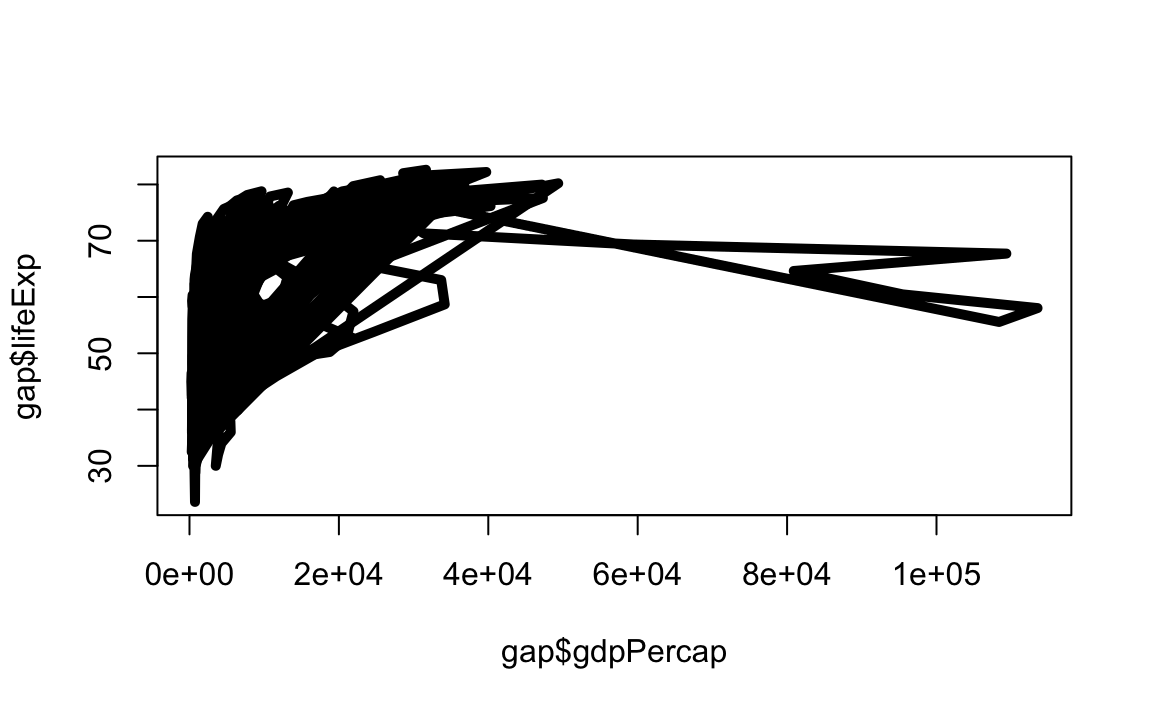
\includegraphics[width=0.7\linewidth]{plsc31101_files/figure-latex/unnamed-chunk-192-5} \includegraphics[width=0.7\linewidth]{plsc31101_files/figure-latex/unnamed-chunk-192-6} 

}

\caption{ }\label{fig:unnamed-chunk-192}
\end{figure}

\subsection{Annotations, Reference Lines, and
Legends}\label{annotations-reference-lines-and-legends}

\begin{itemize}
\tightlist
\item
  Text
\end{itemize}

We can add text to an arbitrary point on the graph like this:

\begin{Shaded}
\begin{Highlighting}[]
\CommentTok{# Plot the line first}
\KeywordTok{plot}\NormalTok{(}\DataTypeTok{x =}\NormalTok{ gap}\OperatorTok{$}\NormalTok{gdpPercap, }\DataTypeTok{y =}\NormalTok{ gap}\OperatorTok{$}\NormalTok{lifeExp, }\DataTypeTok{type=}\StringTok{"p"}\NormalTok{)}
\CommentTok{# Now add the label}
\KeywordTok{text}\NormalTok{(}\DataTypeTok{x=}\DecValTok{40000}\NormalTok{, }\DataTypeTok{y=}\DecValTok{50}\NormalTok{, }\DataTypeTok{labels=}\StringTok{"Evens Out"}\NormalTok{, }\DataTypeTok{cex =}\NormalTok{ .}\DecValTok{75}\NormalTok{)}
\end{Highlighting}
\end{Shaded}

\begin{figure}

{\centering \includegraphics[width=0.7\linewidth]{plsc31101_files/figure-latex/unnamed-chunk-193-1} 

}

\caption{ }\label{fig:unnamed-chunk-193}
\end{figure}

We can also add labels for every point by passing in a vector of text:

\begin{Shaded}
\begin{Highlighting}[]
\CommentTok{# First randomly select rows for a smaller gapaset}
\NormalTok{small <-}\StringTok{ }\NormalTok{gap }\OperatorTok\StringTok{ }\KeywordTok{sample_n}\NormalTok{(}\DecValTok{100}\NormalTok{)}

\CommentTok{# Plot the line first}
\KeywordTok{plot}\NormalTok{(}\DataTypeTok{x =}\NormalTok{ small}\OperatorTok{$}\NormalTok{gdpPercap, }\DataTypeTok{y =}\NormalTok{ small}\OperatorTok{$}\NormalTok{lifeExp, }\DataTypeTok{type=}\StringTok{"p"}\NormalTok{)}
\CommentTok{# Now add the label}
\KeywordTok{text}\NormalTok{(}\DataTypeTok{x =}\NormalTok{ small}\OperatorTok{$}\NormalTok{gdpPercap, }\DataTypeTok{y =}\NormalTok{ small}\OperatorTok{$}\NormalTok{lifeExp, }\DataTypeTok{labels =}\NormalTok{ small}\OperatorTok{$}\NormalTok{country)}
\end{Highlighting}
\end{Shaded}

\begin{figure}

{\centering \includegraphics[width=0.7\linewidth]{plsc31101_files/figure-latex/unnamed-chunk-194-1} 

}

\caption{ }\label{fig:unnamed-chunk-194}
\end{figure}

\begin{itemize}
\tightlist
\item
  Reference Lines
\end{itemize}

\begin{Shaded}
\begin{Highlighting}[]
\CommentTok{# Plot the line}
\KeywordTok{plot}\NormalTok{(}\DataTypeTok{x =}\NormalTok{ gap}\OperatorTok{$}\NormalTok{gdpPercap, }\DataTypeTok{y =}\NormalTok{ gap}\OperatorTok{$}\NormalTok{lifeExp, }\DataTypeTok{type=}\StringTok{"p"}\NormalTok{)}
\CommentTok{# Now the guides}
\KeywordTok{abline}\NormalTok{(}\DataTypeTok{v=}\DecValTok{40000}\NormalTok{, }\DataTypeTok{h=}\DecValTok{75}\NormalTok{, }\DataTypeTok{lty=}\DecValTok{2}\NormalTok{)}
\end{Highlighting}
\end{Shaded}

\begin{figure}

{\centering \includegraphics[width=0.7\linewidth]{plsc31101_files/figure-latex/unnamed-chunk-195-1} 

}

\caption{ }\label{fig:unnamed-chunk-195}
\end{figure}

\begin{Shaded}
\begin{Highlighting}[]
\KeywordTok{library}\NormalTok{(tidyverse)}
\KeywordTok{library}\NormalTok{(gapminder)}

\NormalTok{gap <-}\StringTok{ }\NormalTok{gapminder}
\end{Highlighting}
\end{Shaded}

\section{ggplot2}\label{ggplot2}

\subsubsection*{\texorpdfstring{Why
\texttt{ggplot}?}{Why ggplot?}}\label{why-ggplot}
\addcontentsline{toc}{subsubsection}{Why \texttt{ggplot}?}

\begin{itemize}
\tightlist
\item
  More elegant and compact code than R base graphics.
\item
  More aesthetically pleasing defaults than \texttt{lattice}.
\item
  Very powerful for exploratory data analysis.
\item
  Follows a grammar, just like any language.
\item
  It defines basic components that make up a sentence. In this case, the
  grammar defines components in a plot.
\item
  \emph{G}rammar of \emph{g}raphics originally coined by Lee Wilkinson.
\end{itemize}

\subsection{Grammar}\label{grammar}

The general call for \texttt{ggplot2} looks like this:

\begin{Shaded}
\begin{Highlighting}[]
\KeywordTok{ggplot}\NormalTok{(}\DataTypeTok{data=}\NormalTok{, }\KeywordTok{aes}\NormalTok{(}\DataTypeTok{x=}\NormalTok{, }\DataTypeTok{y=}\NormalTok{), }\DataTypeTok{color=}\NormalTok{, }\DataTypeTok{size=}\NormalTok{,) }\OperatorTok{+}\StringTok{ }\KeywordTok{geom_xxxx}\NormalTok{()}\OperatorTok{+}\KeywordTok{geom_yyyy}\NormalTok{()}
\end{Highlighting}
\end{Shaded}

The \emph{grammar} involves some basic components:

\begin{enumerate}
\def\labelenumi{\arabic{enumi}.}
\tightlist
\item
  \textbf{Data}: A dataframe.
\item
  \textbf{Aes}thetics: How your data are represented visually, i.e., its
  ``mapping.'' Which variables are shown on the x- and y-axes, as well
  as color, size, shape, etc.
\item
  \textbf{Geom}etry: The geometric objects in a plot -- points, lines,
  polygons, etc.
\end{enumerate}

The key to understanding \texttt{ggplot2} is thinking about a figure in
layers, just like you might do in an image editing program like
Photoshop, Illustrator, or Inkscape.

Let's look at an example:

\begin{Shaded}
\begin{Highlighting}[]
\KeywordTok{ggplot}\NormalTok{(}\DataTypeTok{data =}\NormalTok{ gap, }\KeywordTok{aes}\NormalTok{(}\DataTypeTok{x =}\NormalTok{ gdpPercap, }\DataTypeTok{y =}\NormalTok{ lifeExp)) }\OperatorTok{+}
\StringTok{  }\KeywordTok{geom_point}\NormalTok{()}
\end{Highlighting}
\end{Shaded}

\begin{center}\includegraphics[width=0.7\linewidth]{plsc31101_files/figure-latex/unnamed-chunk-199-1} \end{center}

So the first thing we do is call the \texttt{ggplot} function. This
function lets R know that we are creating a new plot, and any of the
arguments we give the \texttt{ggplot} function are the global options
for the plot: They apply to all layers on the plot.

We have passed in two arguments to \texttt{ggplot}. First, we told
\texttt{ggplot} what \textbf{\texttt{data}} we wanted to show on our
figure -- in this example, the \texttt{gapminder} data we read in
earlier.

For the second argument, we passed in the \textbf{\texttt{aes}}
function, which tells \texttt{ggplot} how variables in the data map to
aesthetic properties of the figure -- in this case, the x and y
locations. Here we told \texttt{ggplot} we wanted to plot the
\texttt{lifeExp} column of the \texttt{gapminder} dataframe on the
x-axis, and the \texttt{gdpPercap} column on the y-axis.

Notice that we did not need to explicitly pass \texttt{aes} these
columns (e.g., \texttt{x\ =\ gapminder\$lifeExp}). This is because
\texttt{ggplot} is smart enough to know to look in the data for that
column!

By itself, the call to \texttt{ggplot} is not enough to draw a figure:

\begin{Shaded}
\begin{Highlighting}[]
\KeywordTok{ggplot}\NormalTok{(}\DataTypeTok{data =}\NormalTok{ gap, }\KeywordTok{aes}\NormalTok{(}\DataTypeTok{x =}\NormalTok{ gdpPercap, }\DataTypeTok{y =}\NormalTok{ lifeExp))}
\end{Highlighting}
\end{Shaded}

We need to tell \texttt{ggplot} how we want to visually represent the
data, which we do by adding a new \textbf{\texttt{geom}} layer. In our
example, we used \texttt{geom\_point}, which tells \texttt{ggplot} we
want to visually represent the relationship between x and y as a
scatterplot of points:

\begin{Shaded}
\begin{Highlighting}[]
\KeywordTok{ggplot}\NormalTok{(}\DataTypeTok{data =}\NormalTok{ gap, }\KeywordTok{aes}\NormalTok{(}\DataTypeTok{x =}\NormalTok{ gdpPercap, }\DataTypeTok{y =}\NormalTok{ lifeExp)) }\OperatorTok{+}\StringTok{ }
\StringTok{  }\KeywordTok{geom_point}\NormalTok{()}

\CommentTok{# Same as}
\CommentTok{# my_plot <- ggplot(data = gap, aes(x = gdpPercap, y = lifeExp))}
\CommentTok{# my_plot + geom_point()}
\end{Highlighting}
\end{Shaded}

\begin{center}\includegraphics[width=0.7\linewidth]{plsc31101_files/figure-latex/unnamed-chunk-201-1} \end{center}

\subsubsection*{Challenge 1.}\label{challenge-1.-6}
\addcontentsline{toc}{subsubsection}{Challenge 1.}

Modify the example so that the figure visualizes how life expectancy has
changed over time.

Hint: The \texttt{gapminder} dataset has a column called \texttt{year},
which should appear on the x-axis.

\subsection{\texorpdfstring{Anatomy of
\texttt{aes}}{Anatomy of aes}}\label{anatomy-of-aes}

In the previous examples and challenge, we have used the \texttt{aes}
function to tell the scatterplot \texttt{geom} about the \textbf{x} and
\textbf{y} locations of each point. Another aesthetic property we can
modify is the point \textbf{color}.

\begin{Shaded}
\begin{Highlighting}[]
\KeywordTok{ggplot}\NormalTok{(}\DataTypeTok{data =}\NormalTok{ gap, }\KeywordTok{aes}\NormalTok{(}\DataTypeTok{x =}\NormalTok{ gdpPercap, }\DataTypeTok{y =}\NormalTok{ lifeExp, }\DataTypeTok{color=}\NormalTok{continent)) }\OperatorTok{+}\StringTok{ }
\StringTok{  }\KeywordTok{geom_point}\NormalTok{()}
\end{Highlighting}
\end{Shaded}

\begin{center}\includegraphics[width=0.7\linewidth]{plsc31101_files/figure-latex/unnamed-chunk-202-1} \end{center}

Normally, specifying options like \texttt{color="red"} or
\texttt{size=10} for a given layer results in its contents being red and
quite large. Inside the \texttt{aes()} function, however, these
arguments are given entire variables whose values will then be displayed
using different realizations of that aesthetic.

\textbf{Color} is not the only aesthetic argument we can set to display
variation in the data. We can also vary by shape, size, etc.

\begin{Shaded}
\begin{Highlighting}[]
\KeywordTok{ggplot}\NormalTok{(}\DataTypeTok{data=}\NormalTok{, }\KeywordTok{aes}\NormalTok{(}\DataTypeTok{x=}\NormalTok{, }\DataTypeTok{y=}\NormalTok{, }\DataTypeTok{by =}\NormalTok{, }\DataTypeTok{color=}\NormalTok{, }\DataTypeTok{linetype=}\NormalTok{, }\DataTypeTok{shape=}\NormalTok{, }\DataTypeTok{size=}\NormalTok{))}
\end{Highlighting}
\end{Shaded}

\subsection{Layers}\label{layers}

In the previous challenge, you plotted \texttt{lifExp} over time. Using
a scatterplot probably is not the best for visualizing change over time.
Instead, let's tell \texttt{ggplot} to visualize the data as a line
plot:

\begin{Shaded}
\begin{Highlighting}[]
\KeywordTok{ggplot}\NormalTok{(}\DataTypeTok{data =}\NormalTok{ gap, }\KeywordTok{aes}\NormalTok{(}\DataTypeTok{x=}\NormalTok{year, }\DataTypeTok{y=}\NormalTok{lifeExp, }\DataTypeTok{by=}\NormalTok{country, }\DataTypeTok{color=}\NormalTok{continent)) }\OperatorTok{+}\StringTok{ }
\StringTok{  }\KeywordTok{geom_line}\NormalTok{()}
\end{Highlighting}
\end{Shaded}

\begin{center}\includegraphics[width=0.7\linewidth]{plsc31101_files/figure-latex/unnamed-chunk-204-1} \end{center}

Instead of adding a \texttt{geom\_point} layer, we have added a
\texttt{geom\_line} layer. We have also added the \texttt{**by**}
aesthetic, which tells \texttt{ggplot} to draw a line for each country.

But what if we want to visualize both lines and points on the plot? We
can simply add another layer to the plot:

\begin{Shaded}
\begin{Highlighting}[]
\KeywordTok{ggplot}\NormalTok{(}\DataTypeTok{data =}\NormalTok{ gap, }\KeywordTok{aes}\NormalTok{(}\DataTypeTok{x=}\NormalTok{year, }\DataTypeTok{y=}\NormalTok{lifeExp, }\DataTypeTok{by=}\NormalTok{country, }\DataTypeTok{color=}\NormalTok{continent)) }\OperatorTok{+}\StringTok{ }
\StringTok{  }\KeywordTok{geom_line}\NormalTok{() }\OperatorTok{+}\StringTok{ }
\StringTok{  }\KeywordTok{geom_point}\NormalTok{()}
\end{Highlighting}
\end{Shaded}

\begin{center}\includegraphics[width=0.7\linewidth]{plsc31101_files/figure-latex/unnamed-chunk-205-1} \end{center}

It is important to note that each layer is drawn on top of the previous
layer. In this example, the points have been drawn on top of the lines.
Here is a demonstration:

\begin{Shaded}
\begin{Highlighting}[]
\KeywordTok{ggplot}\NormalTok{(}\DataTypeTok{data =}\NormalTok{ gap, }\KeywordTok{aes}\NormalTok{(}\DataTypeTok{x=}\NormalTok{year, }\DataTypeTok{y=}\NormalTok{lifeExp, }\DataTypeTok{by=}\NormalTok{country)) }\OperatorTok{+}\StringTok{ }
\StringTok{  }\KeywordTok{geom_line}\NormalTok{(}\KeywordTok{aes}\NormalTok{(}\DataTypeTok{color=}\NormalTok{continent)) }\OperatorTok{+}\StringTok{ }
\StringTok{  }\KeywordTok{geom_point}\NormalTok{()}
\end{Highlighting}
\end{Shaded}

\begin{center}\includegraphics[width=0.7\linewidth]{plsc31101_files/figure-latex/unnamed-chunk-206-1} \end{center}

In this example, the aesthetic mapping of \textbf{color} has been moved
from the global plot options in \texttt{ggplot} to the
\texttt{geom\_line} layer, so it no longer applies to the points. Now we
can clearly see that the points are drawn on top of the lines.

\subsubsection*{Challenge 2.}\label{challenge-2.-5}
\addcontentsline{toc}{subsubsection}{Challenge 2.}

Switch the order of the point and line layers from the previous example.
What happened?

\subsection{Labels}\label{labels-1}

Labels are considered to be their own layers in \texttt{ggplot}.

\begin{Shaded}
\begin{Highlighting}[]
\CommentTok{# Add x- and y-axis labels}
\KeywordTok{ggplot}\NormalTok{(}\DataTypeTok{data =}\NormalTok{ gap, }\KeywordTok{aes}\NormalTok{(}\DataTypeTok{x =}\NormalTok{ gdpPercap, }\DataTypeTok{y =}\NormalTok{ lifeExp, }\DataTypeTok{color=}\NormalTok{continent)) }\OperatorTok{+}\StringTok{ }
\StringTok{  }\KeywordTok{geom_point}\NormalTok{() }\OperatorTok{+}\StringTok{ }
\StringTok{  }\KeywordTok{xlab}\NormalTok{(}\StringTok{"GDP per capita"}\NormalTok{) }\OperatorTok{+}\StringTok{ }
\StringTok{  }\KeywordTok{ylab}\NormalTok{(}\StringTok{"Life Expectancy"}\NormalTok{) }\OperatorTok{+}\StringTok{ }
\StringTok{  }\KeywordTok{ggtitle}\NormalTok{(}\StringTok{"My fancy graph"}\NormalTok{)}
\end{Highlighting}
\end{Shaded}

\begin{center}\includegraphics[width=0.7\linewidth]{plsc31101_files/figure-latex/unnamed-chunk-207-1} \end{center}

So are scales:

\begin{Shaded}
\begin{Highlighting}[]
\CommentTok{# Limit x-axis from 1,000 to 20,000}
\KeywordTok{ggplot}\NormalTok{(}\DataTypeTok{data =}\NormalTok{ gap, }\KeywordTok{aes}\NormalTok{(}\DataTypeTok{x =}\NormalTok{ gdpPercap, }\DataTypeTok{y =}\NormalTok{ lifeExp, }\DataTypeTok{color=}\NormalTok{continent)) }\OperatorTok{+}\StringTok{ }
\StringTok{  }\KeywordTok{geom_point}\NormalTok{() }\OperatorTok{+}\StringTok{ }
\StringTok{  }\KeywordTok{xlab}\NormalTok{(}\StringTok{"GDP per capita"}\NormalTok{) }\OperatorTok{+}\StringTok{ }
\StringTok{  }\KeywordTok{ylab}\NormalTok{(}\StringTok{"Life Expectancy"}\NormalTok{) }\OperatorTok{+}\StringTok{ }
\StringTok{  }\KeywordTok{ggtitle}\NormalTok{(}\StringTok{"My fancy graph"}\NormalTok{) }\OperatorTok{+}\StringTok{ }
\StringTok{  }\KeywordTok{xlim}\NormalTok{(}\DecValTok{1000}\NormalTok{, }\DecValTok{20000}\NormalTok{)}
\CommentTok{#> Warning: Removed 515 rows containing missing values (geom_point).}
\end{Highlighting}
\end{Shaded}

\begin{center}\includegraphics[width=0.7\linewidth]{plsc31101_files/figure-latex/unnamed-chunk-208-1} \end{center}

\subsection{Transformations and Stats}\label{transformations-and-stats}

\texttt{ggplot} also makes it easy to overlay statistical models over
the data. To demonstrate, we will go back to an earlier example:

\begin{Shaded}
\begin{Highlighting}[]
\KeywordTok{ggplot}\NormalTok{(}\DataTypeTok{data =}\NormalTok{ gap, }\KeywordTok{aes}\NormalTok{(}\DataTypeTok{x =}\NormalTok{ gdpPercap, }\DataTypeTok{y =}\NormalTok{ lifeExp, }\DataTypeTok{color=}\NormalTok{continent)) }\OperatorTok{+}\StringTok{ }
\StringTok{  }\KeywordTok{geom_point}\NormalTok{()}
\end{Highlighting}
\end{Shaded}

\begin{center}\includegraphics[width=0.7\linewidth]{plsc31101_files/figure-latex/unnamed-chunk-209-1} \end{center}

We can change the scale of units on the x-axis using the \texttt{scale}
functions, which control the mapping between the data values and visual
values of an aesthetic.

\begin{Shaded}
\begin{Highlighting}[]
\KeywordTok{ggplot}\NormalTok{(}\DataTypeTok{data =}\NormalTok{ gap, }\KeywordTok{aes}\NormalTok{(}\DataTypeTok{x =}\NormalTok{ gdpPercap, }\DataTypeTok{y =}\NormalTok{ lifeExp, }\DataTypeTok{color=}\NormalTok{continent)) }\OperatorTok{+}\StringTok{ }
\StringTok{  }\KeywordTok{geom_point}\NormalTok{() }\OperatorTok{+}\StringTok{ }
\StringTok{  }\KeywordTok{scale_x_log10}\NormalTok{()}
\end{Highlighting}
\end{Shaded}

\begin{center}\includegraphics[width=0.7\linewidth]{plsc31101_files/figure-latex/unnamed-chunk-210-1} \end{center}

The \texttt{log10} function applied a transformation to the values of
the \texttt{gdpPercap} column before rendering them on the plot, so that
each multiple of 10 now only corresponds to an increase in 1 on the
transformed scale, e.g., a GDP per capita of 1,000 is now 3 on the
y-axis, a value of 10,000 corresponds to 4 on the x-axis, and so on.
This makes it easier to visualize the spread of data on the x-axis.

We can fit a simple relationship to the data by adding another layer,
\texttt{geom\_smooth}:

\begin{Shaded}
\begin{Highlighting}[]
\KeywordTok{ggplot}\NormalTok{(}\DataTypeTok{data =}\NormalTok{ gap, }\KeywordTok{aes}\NormalTok{(}\DataTypeTok{x =}\NormalTok{ gdpPercap, }\DataTypeTok{y =}\NormalTok{ lifeExp, }\DataTypeTok{color=}\NormalTok{continent)) }\OperatorTok{+}\StringTok{ }
\StringTok{  }\KeywordTok{geom_point}\NormalTok{() }\OperatorTok{+}\StringTok{ }
\StringTok{  }\KeywordTok{scale_x_log10}\NormalTok{() }\OperatorTok{+}\StringTok{ }
\StringTok{  }\KeywordTok{geom_smooth}\NormalTok{(}\DataTypeTok{method=}\StringTok{"lm"}\NormalTok{)}
\CommentTok{#> `geom_smooth()` using formula 'y ~ x'}
\end{Highlighting}
\end{Shaded}

\begin{center}\includegraphics[width=0.7\linewidth]{plsc31101_files/figure-latex/unnamed-chunk-211-1} \end{center}

Note that we have 5 lines, one for each region, because of the
\textbf{\texttt{color}} option in the global \texttt{aes} function. But
if we move it, we get different results:

\begin{Shaded}
\begin{Highlighting}[]
\KeywordTok{ggplot}\NormalTok{(}\DataTypeTok{data =}\NormalTok{ gap, }\KeywordTok{aes}\NormalTok{(}\DataTypeTok{x =}\NormalTok{ gdpPercap, }\DataTypeTok{y =}\NormalTok{ lifeExp)) }\OperatorTok{+}\StringTok{ }
\StringTok{  }\KeywordTok{geom_point}\NormalTok{(}\KeywordTok{aes}\NormalTok{(}\DataTypeTok{color=}\NormalTok{continent)) }\OperatorTok{+}\StringTok{ }
\StringTok{  }\KeywordTok{scale_x_log10}\NormalTok{() }\OperatorTok{+}\StringTok{ }
\StringTok{  }\KeywordTok{geom_smooth}\NormalTok{(}\DataTypeTok{method=}\StringTok{"lm"}\NormalTok{)}
\CommentTok{#> `geom_smooth()` using formula 'y ~ x'}
\end{Highlighting}
\end{Shaded}

\begin{center}\includegraphics[width=0.7\linewidth]{plsc31101_files/figure-latex/unnamed-chunk-212-1} \end{center}

So, there are two ways an aesthetic can be specified. Here, we set the
\textbf{\texttt{color}} aesthetic by passing it as an argument to
\texttt{geom\_point}. Previously in the lesson, we used the \texttt{aes}
function to define a \emph{mapping} between data variables and their
visual representation.

We can make the line thicker by setting the \textbf{\texttt{size}}
aesthetic in the \texttt{geom\_smooth} layer:

\begin{Shaded}
\begin{Highlighting}[]
\KeywordTok{ggplot}\NormalTok{(}\DataTypeTok{data =}\NormalTok{ gap, }\KeywordTok{aes}\NormalTok{(}\DataTypeTok{x =}\NormalTok{ gdpPercap, }\DataTypeTok{y =}\NormalTok{ lifeExp)) }\OperatorTok{+}\StringTok{ }
\StringTok{  }\KeywordTok{geom_point}\NormalTok{(}\KeywordTok{aes}\NormalTok{(}\DataTypeTok{color=}\NormalTok{continent)) }\OperatorTok{+}\StringTok{ }
\StringTok{  }\KeywordTok{scale_x_log10}\NormalTok{() }\OperatorTok{+}\StringTok{ }
\StringTok{  }\KeywordTok{geom_smooth}\NormalTok{(}\DataTypeTok{method=}\StringTok{"lm"}\NormalTok{, }\DataTypeTok{size =} \FloatTok{1.5}\NormalTok{)}
\CommentTok{#> `geom_smooth()` using formula 'y ~ x'}
\end{Highlighting}
\end{Shaded}

\begin{center}\includegraphics[width=0.7\linewidth]{plsc31101_files/figure-latex/unnamed-chunk-213-1} \end{center}

\subsubsection*{Challenge 3.}\label{challenge-3.-3}
\addcontentsline{toc}{subsubsection}{Challenge 3.}

Modify the color and size of the points on the point layer in the
previous example so that they are fixed (i.e., not reflective of
continent).

Hint: Do not use the \texttt{aes} function.

\subsection{Facets}\label{facets}

Earlier, we visualized the change in life expectancy over time across
all countries in one plot. Alternatively, we can split this out over
multiple panels by adding a layer of \textbf{facet} panels:

\begin{Shaded}
\begin{Highlighting}[]
\KeywordTok{ggplot}\NormalTok{(}\DataTypeTok{data =}\NormalTok{ gap, }\KeywordTok{aes}\NormalTok{(}\DataTypeTok{x =}\NormalTok{ year, }\DataTypeTok{y =}\NormalTok{ lifeExp)) }\OperatorTok{+}
\StringTok{  }\KeywordTok{geom_point}\NormalTok{() }\OperatorTok{+}\StringTok{ }
\StringTok{  }\KeywordTok{facet_wrap}\NormalTok{( }\OperatorTok{~}\StringTok{ }\NormalTok{continent)}
\end{Highlighting}
\end{Shaded}

\begin{center}\includegraphics[width=0.7\linewidth]{plsc31101_files/figure-latex/unnamed-chunk-214-1} \end{center}

\subsection{Legend and Scale
Manipulations}\label{legend-and-scale-manipulations}

When creating plots with \texttt{ggplot}, you will notice that legends
are sometimes automatically produced. Additionally, you will often need
to transform the axis scales, similar to the modifcations we made with
the base plots.

We can easily set axis limits with \texttt{xlim} and \texttt{ylim}
layers, or with the \texttt{limits} argument withing
\texttt{scale\_x\_log10}:

\begin{Shaded}
\begin{Highlighting}[]
\KeywordTok{ggplot}\NormalTok{(}\DataTypeTok{data =}\NormalTok{ gap, }\KeywordTok{aes}\NormalTok{(}\DataTypeTok{x =}\NormalTok{ gdpPercap, }\DataTypeTok{y =}\NormalTok{ lifeExp)) }\OperatorTok{+}
\StringTok{  }\KeywordTok{geom_point}\NormalTok{() }\OperatorTok{+}\StringTok{ }
\StringTok{  }\KeywordTok{scale_x_log10}\NormalTok{(}\DataTypeTok{limits =} \KeywordTok{c}\NormalTok{(}\DecValTok{100}\NormalTok{, }\DecValTok{100000}\NormalTok{)) }\OperatorTok{+}
\StringTok{  }\KeywordTok{ylim}\NormalTok{(}\DecValTok{0}\NormalTok{, }\DecValTok{100}\NormalTok{)}
\CommentTok{#> Warning: Removed 3 rows containing missing values (geom_point).}
\end{Highlighting}
\end{Shaded}

\begin{center}\includegraphics[width=0.7\linewidth]{plsc31101_files/figure-latex/unnamed-chunk-215-1} \end{center}

There are many other axis features we can change. For example, we can
change the angle of an axis text with \texttt{theme} or reverse the
direction of an axis with \texttt{scale\_x\_reverse} or
\texttt{scale\_y\_reverse}. Stack Overflow is a great resource for a
variety of axis transformations.

\begin{Shaded}
\begin{Highlighting}[]
\KeywordTok{library}\NormalTok{(scales)}
\CommentTok{#> }
\CommentTok{#> Attaching package: 'scales'}
\CommentTok{#> The following object is masked from 'package:purrr':}
\CommentTok{#> }
\CommentTok{#>     discard}
\CommentTok{#> The following object is masked from 'package:readr':}
\CommentTok{#> }
\CommentTok{#>     col_factor}
\KeywordTok{ggplot}\NormalTok{(}\DataTypeTok{data =}\NormalTok{ gap, }\KeywordTok{aes}\NormalTok{(}\DataTypeTok{x =}\NormalTok{ gdpPercap, }\DataTypeTok{y =}\NormalTok{ lifeExp)) }\OperatorTok{+}
\StringTok{  }\KeywordTok{geom_point}\NormalTok{() }\OperatorTok{+}
\StringTok{  }\KeywordTok{theme}\NormalTok{(}\DataTypeTok{axis.text.x =} \KeywordTok{element_text}\NormalTok{(}\DataTypeTok{angle=}\DecValTok{45}\NormalTok{)) }\OperatorTok{+}
\StringTok{  }\KeywordTok{scale_x_reverse}\NormalTok{()}
\end{Highlighting}
\end{Shaded}

\begin{center}\includegraphics[width=0.7\linewidth]{plsc31101_files/figure-latex/unnamed-chunk-216-1} \end{center}

Legend manipulations can be a little trickier. Let's consider a plot
where we group our observations by continent:

\begin{Shaded}
\begin{Highlighting}[]
\NormalTok{legend_plot <-}\StringTok{ }\KeywordTok{ggplot}\NormalTok{(}\DataTypeTok{data =}\NormalTok{ gap, }\KeywordTok{aes}\NormalTok{(}\DataTypeTok{x =} \KeywordTok{log}\NormalTok{(gdpPercap), }\DataTypeTok{y =}\NormalTok{ lifeExp, }\DataTypeTok{color=}\NormalTok{continent)) }\OperatorTok{+}
\StringTok{  }\KeywordTok{geom_point}\NormalTok{() }\OperatorTok{+}\StringTok{ }
\StringTok{  }\KeywordTok{scale_x_log10}\NormalTok{()}

\NormalTok{legend_plot}
\end{Highlighting}
\end{Shaded}

\begin{center}\includegraphics[width=0.7\linewidth]{plsc31101_files/figure-latex/unnamed-chunk-217-1} \end{center}

First, let's change the legend position:

\begin{Shaded}
\begin{Highlighting}[]
\NormalTok{legend_plot }\OperatorTok{+}\StringTok{ }
\StringTok{  }\KeywordTok{theme}\NormalTok{(}\DataTypeTok{legend.position=}\StringTok{"bottom"}\NormalTok{)}

\NormalTok{legend_plot }\OperatorTok{+}\StringTok{ }
\StringTok{  }\KeywordTok{theme}\NormalTok{(}\DataTypeTok{legend.position=}\StringTok{"top"}\NormalTok{)}
\end{Highlighting}
\end{Shaded}

\begin{center}\includegraphics[width=0.7\linewidth]{plsc31101_files/figure-latex/unnamed-chunk-218-1} \includegraphics[width=0.7\linewidth]{plsc31101_files/figure-latex/unnamed-chunk-218-2} \end{center}

We can also remove the title of the legend for self-explanatory
groupings:

\begin{Shaded}
\begin{Highlighting}[]
\NormalTok{legend_plot }\OperatorTok{+}\StringTok{ }
\StringTok{  }\KeywordTok{theme}\NormalTok{(}\DataTypeTok{legend.title =} \KeywordTok{element_blank}\NormalTok{())}
\end{Highlighting}
\end{Shaded}

\begin{center}\includegraphics[width=0.7\linewidth]{plsc31101_files/figure-latex/unnamed-chunk-219-1} \end{center}

We can reverse the order of the groups with the \texttt{guides} layer.
Here, we specify that we want to reverse \texttt{color}, because that
was the original aesthetic that we specified to create the groupings and
the legend:

\begin{Shaded}
\begin{Highlighting}[]
\NormalTok{legend_plot }\OperatorTok{+}
\StringTok{  }\KeywordTok{guides}\NormalTok{(}\DataTypeTok{color =} \KeywordTok{guide_legend}\NormalTok{(}\DataTypeTok{reverse =} \OtherTok{TRUE}\NormalTok{))}
\end{Highlighting}
\end{Shaded}

\begin{center}\includegraphics[width=0.7\linewidth]{plsc31101_files/figure-latex/unnamed-chunk-220-1} \end{center}

Finally, we can also change the legend title by modifying the label for
\texttt{color}:

\begin{Shaded}
\begin{Highlighting}[]
\NormalTok{legend_plot }\OperatorTok{+}
\StringTok{  }\KeywordTok{labs}\NormalTok{(}\DataTypeTok{color =} \StringTok{"My New Title"}\NormalTok{)}
\end{Highlighting}
\end{Shaded}

\begin{center}\includegraphics[width=0.7\linewidth]{plsc31101_files/figure-latex/unnamed-chunk-221-1} \end{center}

And we can change the legend labels and colors. Again, we are using
\texttt{scale\_color\_manual} because we originally specified the groups
with the \texttt{**color**} aesthetic:

\begin{Shaded}
\begin{Highlighting}[]
\NormalTok{legend_plot }\OperatorTok{+}
\StringTok{  }\KeywordTok{scale_color_manual}\NormalTok{(}\DataTypeTok{labels =} \KeywordTok{c}\NormalTok{(}\StringTok{"Af"}\NormalTok{, }\StringTok{"Am"}\NormalTok{, }\StringTok{"As"}\NormalTok{, }\StringTok{"Eu"}\NormalTok{, }\StringTok{"Oc"}\NormalTok{), }
                     \DataTypeTok{values =} \KeywordTok{c}\NormalTok{(}\StringTok{"red"}\NormalTok{, }\StringTok{"darkblue"}\NormalTok{, }\StringTok{"seagreen"}\NormalTok{, }\StringTok{"purple"}\NormalTok{, }\StringTok{"#5ab4ac"}\NormalTok{))}
\end{Highlighting}
\end{Shaded}

\begin{center}\includegraphics[width=0.7\linewidth]{plsc31101_files/figure-latex/unnamed-chunk-222-1} \end{center}

\subsection{Putting Everything
Together}\label{putting-everything-together}

Here are some other common \texttt{geom} layers:

\textbf{Bar Plots}

\begin{Shaded}
\begin{Highlighting}[]
\CommentTok{# Count of lifeExp bins}
\KeywordTok{ggplot}\NormalTok{(}\DataTypeTok{data =}\NormalTok{ gap, }\KeywordTok{aes}\NormalTok{(}\DataTypeTok{x =}\NormalTok{ lifeExp)) }\OperatorTok{+}\StringTok{ }
\StringTok{  }\KeywordTok{geom_bar}\NormalTok{(}\DataTypeTok{stat=}\StringTok{"bin"}\NormalTok{)}
\CommentTok{#> `stat_bin()` using `bins = 30`. Pick better value with `binwidth`.}

\CommentTok{# With color representing regions}
\KeywordTok{ggplot}\NormalTok{(}\DataTypeTok{data =}\NormalTok{ gap, }\KeywordTok{aes}\NormalTok{(}\DataTypeTok{x =}\NormalTok{ lifeExp, }\DataTypeTok{fill =}\NormalTok{ continent)) }\OperatorTok{+}\StringTok{ }
\StringTok{  }\KeywordTok{geom_bar}\NormalTok{(}\DataTypeTok{stat=}\StringTok{"bin"}\NormalTok{)}
\CommentTok{#> `stat_bin()` using `bins = 30`. Pick better value with `binwidth`.}
\end{Highlighting}
\end{Shaded}

\begin{center}\includegraphics[width=0.7\linewidth]{plsc31101_files/figure-latex/unnamed-chunk-223-1} \includegraphics[width=0.7\linewidth]{plsc31101_files/figure-latex/unnamed-chunk-223-2} \end{center}

\textbf{Box Plots}

\begin{Shaded}
\begin{Highlighting}[]
\KeywordTok{ggplot}\NormalTok{(}\DataTypeTok{data =}\NormalTok{ gap, }\KeywordTok{aes}\NormalTok{(}\DataTypeTok{x =}\NormalTok{ continent, }\DataTypeTok{y =}\NormalTok{ lifeExp)) }\OperatorTok{+}\StringTok{ }
\StringTok{  }\KeywordTok{geom_boxplot}\NormalTok{()}
\end{Highlighting}
\end{Shaded}

\begin{center}\includegraphics[width=0.7\linewidth]{plsc31101_files/figure-latex/unnamed-chunk-224-1} \end{center}

This is just a taste of what you can do with \texttt{ggplot2}.

RStudio provides a really useful
\href{https://www.rstudio.com/wp-content/uploads/2015/03/ggplot2-cheatsheet.pdf}{cheat
sheet} of the different layers available, and more extensive
documentation is available on the
\href{http://docs.ggplot2.org/current/}{\texttt{ggplot2} website}.

Finally, if you have no idea how to change something, a quick Google
search will usually send you to a relevant question and answer on Stack
Overflow with reusable code to modify!

\subsubsection*{Challenge 4.}\label{challenge-4.-1}
\addcontentsline{toc}{subsubsection}{Challenge 4.}

Create a density plot of GDP per capita, filled by continent.

Advanced:

\begin{itemize}
\tightlist
\item
  Transform the x-axis to better visualize the data spread.
\item
  Add a facet layer to panel the density plots by year.
\end{itemize}

\section{Saving Plots}\label{saving-plots}

There are two basic image types:

\begin{enumerate}
\def\labelenumi{\arabic{enumi})}
\tightlist
\item
  \textbf{Raster/Bitmap} (.png, .jpeg)
\end{enumerate}

Every pixel of a plot contains its own separate coding; not so great if
you want to resize the image.

\begin{Shaded}
\begin{Highlighting}[]
\KeywordTok{jpeg}\NormalTok{(}\DataTypeTok{filename=}\StringTok{"example.png"}\NormalTok{, }\DataTypeTok{width=}\NormalTok{, }\DataTypeTok{height=}\NormalTok{)}
\KeywordTok{plot}\NormalTok{(x,y)}
\KeywordTok{dev.off}\NormalTok{()}
\end{Highlighting}
\end{Shaded}

\begin{enumerate}
\def\labelenumi{\arabic{enumi})}
\setcounter{enumi}{1}
\tightlist
\item
  \textbf{Vector} (.pdf, .ps)
\end{enumerate}

Every element of a plot is encoded with a function that gives its coding
conditional on several factors; this is great for resizing.

\begin{Shaded}
\begin{Highlighting}[]
\KeywordTok{pdf}\NormalTok{(}\DataTypeTok{filename=}\StringTok{"example.pdf"}\NormalTok{, }\DataTypeTok{width=}\NormalTok{, }\DataTypeTok{height=}\NormalTok{)}
\KeywordTok{plot}\NormalTok{(x,y)}
\KeywordTok{dev.off}\NormalTok{()}
\end{Highlighting}
\end{Shaded}

\textbf{Exporting with \texttt{ggplot}}

\begin{Shaded}
\begin{Highlighting}[]
\CommentTok{# Assume we saved our plot as an object called example.plot}
\KeywordTok{ggsave}\NormalTok{(}\DataTypeTok{filename=}\StringTok{"example.pdf"}\NormalTok{, }\DataTypeTok{plot=}\NormalTok{example.plot, }\DataTypeTok{scale=}\NormalTok{, }\DataTypeTok{width=}\NormalTok{, }\DataTypeTok{height=}\NormalTok{)}
\end{Highlighting}
\end{Shaded}

\chapter{Statistical Inferences}\label{statistical-inferences}

\begin{Shaded}
\begin{Highlighting}[]
\CommentTok{# setup}
\KeywordTok{library}\NormalTok{(gapminder)}
\NormalTok{gap <-}\StringTok{ }\NormalTok{gapminder}
\end{Highlighting}
\end{Shaded}

\section{Statistical Distributions}\label{statistical-distributions}

Since R was developed by statisticians, it handles distributions and
simulation seamlessly.

All commonly-used distributions have functions in R. Each distribution
has a family of functions:

\begin{itemize}
\tightlist
\item
  \texttt{d} - Probability density/mass function, e.g., \texttt{dnorm()}
\item
  \texttt{r} - Generate a random value, e.g., \texttt{rnorm()}
\item
  \texttt{p} - Cumulative distribution function, e.g., \texttt{pnorm()}
\item
  \texttt{q} - Quantile function (inverse CDF), e.g., \texttt{qnorm()}
\end{itemize}

Let's see some of these functions in action with the normal distribution
(mean 0, standard deviation 1):

\begin{Shaded}
\begin{Highlighting}[]
\KeywordTok{dnorm}\NormalTok{(}\FloatTok{1.96}\NormalTok{) }\CommentTok{# Probability density of 1.96 from the normal distribution}
\CommentTok{#> [1] 0.0584}
\KeywordTok{rnorm}\NormalTok{(}\DecValTok{1}\OperatorTok{:}\DecValTok{10}\NormalTok{) }\CommentTok{# Get 10 random values from the normal distribution}
\CommentTok{#>  [1] -1.40004  0.25532 -2.43726 -0.00557  0.62155  1.14841 -1.82182 -0.24733}
\CommentTok{#>  [9] -0.24420 -0.28271}
\KeywordTok{pnorm}\NormalTok{(}\FloatTok{1.96}\NormalTok{) }\CommentTok{# Cumulative distribution function}
\CommentTok{#> [1] 0.975}
\KeywordTok{qnorm}\NormalTok{(.}\DecValTok{975}\NormalTok{) }\CommentTok{# Inverse cumulative distribution function}
\CommentTok{#> [1] 1.96}
\end{Highlighting}
\end{Shaded}

We can also use these functions on other distributions:

\begin{itemize}
\tightlist
\item
  \texttt{rnorm()} \# Normal distribution
\item
  \texttt{runif()} \# Uniform distribution
\item
  \texttt{rbinom()} \# Binomial distribution
\item
  \texttt{rpois()} \# Poisson distribution
\item
  \texttt{rbeta()} \# Beta distribution
\item
  \texttt{rgamma()} \# Gamma distribution
\item
  \texttt{rt()} \# Student t distribution
\item
  \texttt{rchisq()}. \# Chi-squared distribution
\end{itemize}

\begin{Shaded}
\begin{Highlighting}[]
\KeywordTok{rbinom}\NormalTok{(}\DecValTok{0}\OperatorTok{:}\DecValTok{10}\NormalTok{, }\DataTypeTok{size =} \DecValTok{10}\NormalTok{, }\DataTypeTok{prob =} \FloatTok{0.3}\NormalTok{)}
\CommentTok{#>  [1] 2 4 4 2 6 4 1 3 4 4 1}
\KeywordTok{dt}\NormalTok{(}\DecValTok{5}\NormalTok{, }\DataTypeTok{df =} \DecValTok{1}\NormalTok{)}
\CommentTok{#> [1] 0.0122}

\NormalTok{x <-}\StringTok{ }\KeywordTok{seq}\NormalTok{(}\OperatorTok{-}\DecValTok{5}\NormalTok{, }\DecValTok{5}\NormalTok{, }\DataTypeTok{length =} \DecValTok{100}\NormalTok{)}
\KeywordTok{plot}\NormalTok{(x, }\KeywordTok{dnorm}\NormalTok{(x), }\DataTypeTok{type =} \StringTok{'l'}\NormalTok{)}
\end{Highlighting}
\end{Shaded}

\begin{center}\includegraphics[width=0.7\linewidth]{plsc31101_files/figure-latex/unnamed-chunk-231-1} \end{center}

\subsection{Sampling and Simulation}\label{sampling-and-simulation}

We can draw a sample with or without replacement with \texttt{sample}.

\begin{Shaded}
\begin{Highlighting}[]
\KeywordTok{sample}\NormalTok{(}\DecValTok{1}\OperatorTok{:}\KeywordTok{nrow}\NormalTok{(gap), }\DecValTok{20}\NormalTok{, }\DataTypeTok{replace =} \OtherTok{FALSE}\NormalTok{)}
\CommentTok{#>  [1]  447 1284  752  674 1699 1241  726 1579 1568 1094  265  150 1023 1290 1440}
\CommentTok{#> [16]  117  930 1553  180 1208}
\end{Highlighting}
\end{Shaded}

\texttt{dplyr} has a helpful \texttt{select\_n} function that samples
rows of a dataframe.

\begin{Shaded}
\begin{Highlighting}[]
\NormalTok{small <-}\StringTok{ }\KeywordTok{sample_n}\NormalTok{(gap, }\DecValTok{20}\NormalTok{)}
\KeywordTok{nrow}\NormalTok{(small)}
\CommentTok{#> [1] 20}
\end{Highlighting}
\end{Shaded}

Here's an example of some code that would be part of a bootstrap:

\begin{Shaded}
\begin{Highlighting}[]
\NormalTok{gap <-}\StringTok{ }\KeywordTok{read.csv}\NormalTok{(}\StringTok{"data/gapminder-FiveYearData.csv"}\NormalTok{, }\DataTypeTok{stringsAsFactors =}\NormalTok{ F)}

\CommentTok{# Actual mean}
\KeywordTok{mean}\NormalTok{(gap}\OperatorTok{$}\NormalTok{lifeExp, }\DataTypeTok{na.rm =} \OtherTok{TRUE}\NormalTok{)}
\CommentTok{#> [1] 59.5}

\CommentTok{# Here's a bootstrap sample:}
\NormalTok{smp <-}\StringTok{ }\KeywordTok{sample_n}\NormalTok{(gap, }\DataTypeTok{size =} \KeywordTok{nrow}\NormalTok{(gap), }\DataTypeTok{replace =} \OtherTok{TRUE}\NormalTok{) }
\KeywordTok{mean}\NormalTok{(smp}\OperatorTok{$}\NormalTok{lifeExp, }\DataTypeTok{na.rm =} \OtherTok{TRUE}\NormalTok{)}
\CommentTok{#> [1] 59.4}
\end{Highlighting}
\end{Shaded}

\subsection{Random Seeds}\label{random-seeds}

A few key facts about generating random numbers:

\begin{itemize}
\tightlist
\item
  Random numbers on a computer are \emph{pseudo-random}; they are
  generated deterministically from a very, very, very long sequence that
  repeats.
\item
  The \emph{seed} determines where you are in that sequence.
\end{itemize}

To replicate any work involving random numbers, make sure to set the
seed first. The seed can be arbitrary -- pick your favorite number.

\begin{Shaded}
\begin{Highlighting}[]
\KeywordTok{set.seed}\NormalTok{(}\DecValTok{1}\NormalTok{)}
\NormalTok{vals <-}\StringTok{ }\KeywordTok{sample}\NormalTok{(}\DecValTok{1}\OperatorTok{:}\KeywordTok{nrow}\NormalTok{(gap), }\DecValTok{10}\NormalTok{)}
\NormalTok{vals}
\CommentTok{#>  [1] 1017  679  129  930 1533  471  299  270 1211 1331}

\NormalTok{vals <-}\StringTok{ }\KeywordTok{sample}\NormalTok{(}\DecValTok{1}\OperatorTok{:}\KeywordTok{nrow}\NormalTok{(gap), }\DecValTok{10}\NormalTok{)}
\NormalTok{vals}
\CommentTok{#>  [1]  597 1301 1518  330 1615   37 1129  729  878  485}

\KeywordTok{set.seed}\NormalTok{(}\DecValTok{1}\NormalTok{)}
\NormalTok{vals <-}\StringTok{ }\KeywordTok{sample}\NormalTok{(}\DecValTok{1}\OperatorTok{:}\KeywordTok{nrow}\NormalTok{(gap), }\DecValTok{10}\NormalTok{)}
\NormalTok{vals}
\CommentTok{#>  [1] 1017  679  129  930 1533  471  299  270 1211 1331}
\end{Highlighting}
\end{Shaded}

\subsection{Challenges}\label{challenges-9}

\subsubsection*{Challenge 1.}\label{challenge-1.-7}
\addcontentsline{toc}{subsubsection}{Challenge 1.}

Generate 100 random Poisson values with a population mean of 5. How
close is the mean of those 100 values to the value of 5?

\subsubsection*{Challenge 2.}\label{challenge-2.-6}
\addcontentsline{toc}{subsubsection}{Challenge 2.}

What is the 95th percentile of a chi-square distribution with 1 degree
of freedom?

\subsubsection*{Challenge 3.}\label{challenge-3.-4}
\addcontentsline{toc}{subsubsection}{Challenge 3.}

What is the probability of getting a value greater than 5 if you draw
from a standard normal distribution? What about a t distribution with 1
degree of freedom?

\section{Inferences and Regressions}\label{inferences-and-regressions}

Once we have imported our data, summarized it, carried out group-wise
operations, and perhaps reshaped it, we may also want to attempt causal
inference.

This often requires doing the following:

\begin{enumerate}
\def\labelenumi{\arabic{enumi})}
\tightlist
\item
  Carrying out Classical Hypothesis Tests
\item
  Estimating Regressions
\end{enumerate}

\begin{Shaded}
\begin{Highlighting}[]
\CommentTok{# Setup}
\KeywordTok{library}\NormalTok{(gapminder)}
\NormalTok{gap <-}\StringTok{ }\NormalTok{gapminder}
\end{Highlighting}
\end{Shaded}

\subsection{Statistical Tests}\label{statistical-tests}

Let's say we are interested in whether the life expectancy in 1967 is
different than in 1977.

\begin{Shaded}
\begin{Highlighting}[]
\CommentTok{# Pull out life expectancy by different years}
\NormalTok{life.exp.}\DecValTok{1967}\NormalTok{ <-}\StringTok{ }\NormalTok{gap}\OperatorTok{$}\NormalTok{lifeExp[gap}\OperatorTok{$}\NormalTok{year}\OperatorTok{==}\DecValTok{1967}\NormalTok{]}
\NormalTok{life.exp.}\DecValTok{1977}\NormalTok{ <-}\StringTok{ }\NormalTok{gap}\OperatorTok{$}\NormalTok{lifeExp[gap}\OperatorTok{$}\NormalTok{year}\OperatorTok{==}\DecValTok{1977}\NormalTok{]}
\end{Highlighting}
\end{Shaded}

One can test for differences in distributions in either:

\begin{enumerate}
\def\labelenumi{\arabic{enumi})}
\tightlist
\item
  Their means using t-tests:
\end{enumerate}

\begin{Shaded}
\begin{Highlighting}[]
\CommentTok{# t test of means}
\KeywordTok{t.test}\NormalTok{(}\DataTypeTok{x =}\NormalTok{ life.exp.}\DecValTok{1967}\NormalTok{, }\DataTypeTok{y =}\NormalTok{ life.exp.}\DecValTok{1977}\NormalTok{)}
\CommentTok{#> }
\CommentTok{#>  Welch Two Sample t-test}
\CommentTok{#> }
\CommentTok{#> data:  life.exp.1967 and life.exp.1977}
\CommentTok{#> t = -3, df = 281, p-value = 0.005}
\CommentTok{#> alternative hypothesis: true difference in means is not equal to 0}
\CommentTok{#> 95 percent confidence interval:}
\CommentTok{#>  -6.57 -1.21}
\CommentTok{#> sample estimates:}
\CommentTok{#> mean of x mean of y }
\CommentTok{#>      55.7      59.6}
\end{Highlighting}
\end{Shaded}

\begin{enumerate}
\def\labelenumi{\arabic{enumi})}
\setcounter{enumi}{1}
\tightlist
\item
  Their entire distributions using ks-tests:
\end{enumerate}

\begin{Shaded}
\begin{Highlighting}[]
\CommentTok{# ks tests of distributions}
\KeywordTok{ks.test}\NormalTok{(}\DataTypeTok{x =}\NormalTok{ life.exp.}\DecValTok{1967}\NormalTok{, }\DataTypeTok{y =}\NormalTok{ life.exp.}\DecValTok{1977}\NormalTok{)}
\CommentTok{#> Warning in ks.test(x = life.exp.1967, y = life.exp.1977): p-value will be}
\CommentTok{#> approximate in the presence of ties}
\CommentTok{#> }
\CommentTok{#>  Two-sample Kolmogorov-Smirnov test}
\CommentTok{#> }
\CommentTok{#> data:  life.exp.1967 and life.exp.1977}
\CommentTok{#> D = 0.2, p-value = 0.008}
\CommentTok{#> alternative hypothesis: two-sided}
\end{Highlighting}
\end{Shaded}

\subsection{Regressions and Linear
Models}\label{regressions-and-linear-models}

Running regressions in R is generally straightforward. There are two
basic, catch-all regression functions in R:

\begin{itemize}
\item
  \texttt{glm} fits a generalized linear model with your choice of
  family/link function (Gaussian, logit, Poisson, etc.).
\item
  \texttt{lm} is just a standard linear regression (equivalent to
  \texttt{glm} with \texttt{family\ =\ gaussian(link\ =\ "identity")}).
\end{itemize}

The basic \texttt{glm} call looks something like this:

\begin{Shaded}
\begin{Highlighting}[]
\KeywordTok{glm}\NormalTok{(}\DataTypeTok{formula =}\NormalTok{ y }\OperatorTok{~}\StringTok{ }\NormalTok{x1 }\OperatorTok{+}\StringTok{ }\NormalTok{x2 }\OperatorTok{+}\StringTok{ }\NormalTok{x3 }\OperatorTok{+}\StringTok{ }\NormalTok{..., }\DataTypeTok{family =} \KeywordTok{familyname}\NormalTok{(}\DataTypeTok{link =} \StringTok{"linkname"}\NormalTok{), }\DataTypeTok{data =}\NormalTok{ )}
\end{Highlighting}
\end{Shaded}

There are a bunch of families and links to use (\texttt{?family} for a
full list), but some essentials are:
\textbf{\texttt{binomial(link\ =\ "logit")}},
\textbf{\texttt{gaussian(link\ =\ "identity")}}, and
\textbf{\texttt{poisson(link\ =\ "log")}}.

If you are using \texttt{lm}, the call looks the same but without the
\texttt{family} argument.

\begin{itemize}
\tightlist
\item
  Example: Suppose we want to regress the life expectency on the GDP per
  capita and the population, as well as the continent and the year. The
  \texttt{lm} call would be something like this:
\end{itemize}

\begin{Shaded}
\begin{Highlighting}[]
\NormalTok{reg <-}\StringTok{ }\KeywordTok{lm}\NormalTok{(}\DataTypeTok{formula =}\NormalTok{ lifeExp }\OperatorTok{~}\StringTok{ }\KeywordTok{log}\NormalTok{(gdpPercap) }\OperatorTok{+}\StringTok{ }\KeywordTok{log}\NormalTok{(pop) }\OperatorTok{+}\StringTok{ }\NormalTok{continent }\OperatorTok{+}\StringTok{ }\NormalTok{year, }\DataTypeTok{data =}\NormalTok{ gap)}
\end{Highlighting}
\end{Shaded}

\subsubsection*{Missing values}\label{missing-values}
\addcontentsline{toc}{subsubsection}{Missing values}

Missing values obviously cannot convey any information about the
relationship between the variables. Most modeling functions will drop
any rows that contain missing values.

\subsection{Regression Output}\label{regression-output}

When we store this regression in an object, we get access to several
items of interest:

\begin{enumerate}
\def\labelenumi{\arabic{enumi}.}
\tightlist
\item
  All components contained in the regression output:
\end{enumerate}

\begin{Shaded}
\begin{Highlighting}[]
\KeywordTok{names}\NormalTok{(reg)}
\CommentTok{#>  [1] "coefficients"  "residuals"     "effects"       "rank"         }
\CommentTok{#>  [5] "fitted.values" "assign"        "qr"            "df.residual"  }
\CommentTok{#>  [9] "contrasts"     "xlevels"       "call"          "terms"        }
\CommentTok{#> [13] "model"}
\end{Highlighting}
\end{Shaded}

\begin{enumerate}
\def\labelenumi{\arabic{enumi}.}
\setcounter{enumi}{1}
\tightlist
\item
  Regression coefficients:
\end{enumerate}

\begin{Shaded}
\begin{Highlighting}[]
\NormalTok{reg}\OperatorTok{$}\NormalTok{coefficients}
\CommentTok{#>       (Intercept)    log(gdpPercap)          log(pop) continentAmericas }
\CommentTok{#>          -460.813             5.076             0.153             8.745 }
\CommentTok{#>     continentAsia   continentEurope  continentOceania              year }
\CommentTok{#>             6.825            12.281            12.540             0.238}
\end{Highlighting}
\end{Shaded}

\begin{enumerate}
\def\labelenumi{\arabic{enumi}.}
\setcounter{enumi}{2}
\tightlist
\item
  Regression degrees of freedom:
\end{enumerate}

\begin{Shaded}
\begin{Highlighting}[]
\NormalTok{reg}\OperatorTok{$}\NormalTok{df.residual}
\CommentTok{#> [1] 1696}
\end{Highlighting}
\end{Shaded}

\begin{enumerate}
\def\labelenumi{\arabic{enumi}.}
\setcounter{enumi}{3}
\tightlist
\item
  Standard (diagnostic) plots for a regression:
\end{enumerate}

\begin{Shaded}
\begin{Highlighting}[]
\KeywordTok{plot}\NormalTok{(reg)}
\end{Highlighting}
\end{Shaded}

\begin{center}\includegraphics[width=0.7\linewidth]{plsc31101_files/figure-latex/unnamed-chunk-246-1} \includegraphics[width=0.7\linewidth]{plsc31101_files/figure-latex/unnamed-chunk-246-2} \includegraphics[width=0.7\linewidth]{plsc31101_files/figure-latex/unnamed-chunk-246-3} \includegraphics[width=0.7\linewidth]{plsc31101_files/figure-latex/unnamed-chunk-246-4} \end{center}

R also has a helpful \texttt{summary} method for regression objects:

\begin{Shaded}
\begin{Highlighting}[]
\KeywordTok{summary}\NormalTok{(reg)}
\CommentTok{#> }
\CommentTok{#> Call:}
\CommentTok{#> lm(formula = lifeExp ~ log(gdpPercap) + log(pop) + continent + }
\CommentTok{#>     year, data = gap)}
\CommentTok{#> }
\CommentTok{#> Residuals:}
\CommentTok{#>     Min      1Q  Median      3Q     Max }
\CommentTok{#> -25.057  -3.286   0.329   3.706  15.065 }
\CommentTok{#> }
\CommentTok{#> Coefficients:}
\CommentTok{#>                    Estimate Std. Error t value Pr(>|t|)    }
\CommentTok{#> (Intercept)       -4.61e+02   1.70e+01  -27.15   <2e-16 ***}
\CommentTok{#> log(gdpPercap)     5.08e+00   1.63e-01   31.19   <2e-16 ***}
\CommentTok{#> log(pop)           1.53e-01   9.67e-02    1.58     0.11    }
\CommentTok{#> continentAmericas  8.75e+00   4.77e-01   18.35   <2e-16 ***}
\CommentTok{#> continentAsia      6.83e+00   4.23e-01   16.13   <2e-16 ***}
\CommentTok{#> continentEurope    1.23e+01   5.29e-01   23.20   <2e-16 ***}
\CommentTok{#> continentOceania   1.25e+01   1.28e+00    9.79   <2e-16 ***}
\CommentTok{#> year               2.38e-01   8.93e-03   26.61   <2e-16 ***}
\CommentTok{#> ---}
\CommentTok{#> Signif. codes:  0 '***' 0.001 '**' 0.01 '*' 0.05 '.' 0.1 ' ' 1}
\CommentTok{#> }
\CommentTok{#> Residual standard error: 5.81 on 1696 degrees of freedom}
\CommentTok{#> Multiple R-squared:  0.798,  Adjusted R-squared:  0.798 }
\CommentTok{#> F-statistic:  960 on 7 and 1696 DF,  p-value: <2e-16}
\end{Highlighting}
\end{Shaded}

We can also extract useful things from the summary object:

\begin{Shaded}
\begin{Highlighting}[]
\CommentTok{# Store summary method results}
\NormalTok{summ_reg <-}\StringTok{ }\KeywordTok{summary}\NormalTok{(reg)}

\CommentTok{# View summary method results objects}
\KeywordTok{objects}\NormalTok{(summ_reg)}
\CommentTok{#>  [1] "adj.r.squared" "aliased"       "call"          "coefficients" }
\CommentTok{#>  [5] "cov.unscaled"  "df"            "fstatistic"    "r.squared"    }
\CommentTok{#>  [9] "residuals"     "sigma"         "terms"}

\CommentTok{# View table of coefficients}
\NormalTok{summ_reg}\OperatorTok{$}\NormalTok{coefficients}
\CommentTok{#>                   Estimate Std. Error t value  Pr(>|t|)}
\CommentTok{#> (Intercept)       -460.813   16.97028  -27.15 3.96e-135}
\CommentTok{#> log(gdpPercap)       5.076    0.16272   31.19 3.37e-169}
\CommentTok{#> log(pop)             0.153    0.09668    1.58  1.14e-01}
\CommentTok{#> continentAmericas    8.745    0.47660   18.35  9.61e-69}
\CommentTok{#> continentAsia        6.825    0.42320   16.13  1.49e-54}
\CommentTok{#> continentEurope     12.281    0.52924   23.20 1.12e-103}
\CommentTok{#> continentOceania    12.540    1.28114    9.79  4.80e-22}
\CommentTok{#> year                 0.238    0.00893   26.61 1.06e-130}
\end{Highlighting}
\end{Shaded}

\subsection{Interactions}\label{interactions}

There are also some useful shortcuts for regressing on interaction
terms:

\begin{enumerate}
\def\labelenumi{\arabic{enumi}.}
\tightlist
\item
  \texttt{x1:x2} interacts all terms in \texttt{x1} with all terms in
  \texttt{x2}:
\end{enumerate}

\begin{Shaded}
\begin{Highlighting}[]
\NormalTok{mod.}\DecValTok{1}\NormalTok{ <-}\StringTok{ }\KeywordTok{lm}\NormalTok{(lifeExp }\OperatorTok{~}\StringTok{ }\KeywordTok{log}\NormalTok{(gdpPercap) }\OperatorTok{+}\StringTok{ }\KeywordTok{log}\NormalTok{(pop) }\OperatorTok{+}\StringTok{ }\NormalTok{continent}\OperatorTok{:}\KeywordTok{factor}\NormalTok{(year), }\DataTypeTok{data =}\NormalTok{ gap)}
\KeywordTok{summary}\NormalTok{(mod.}\DecValTok{1}\NormalTok{)}
\CommentTok{#> }
\CommentTok{#> Call:}
\CommentTok{#> lm(formula = lifeExp ~ log(gdpPercap) + log(pop) + continent:factor(year), }
\CommentTok{#>     data = gap)}
\CommentTok{#> }
\CommentTok{#> Residuals:}
\CommentTok{#>     Min      1Q  Median      3Q     Max }
\CommentTok{#> -26.568  -2.553   0.004   2.915  15.567 }
\CommentTok{#> }
\CommentTok{#> Coefficients: (1 not defined because of singularities)}
\CommentTok{#>                                    Estimate Std. Error t value Pr(>|t|)    }
\CommentTok{#> (Intercept)                         27.1838     4.6849    5.80  7.8e-09 ***}
\CommentTok{#> log(gdpPercap)                       5.0795     0.1605   31.65  < 2e-16 ***}
\CommentTok{#> log(pop)                             0.0789     0.0943    0.84  0.40251    }
\CommentTok{#> continentAfrica:factor(year)1952   -24.1425     4.1125   -5.87  5.2e-09 ***}
\CommentTok{#> continentAmericas:factor(year)1952 -16.4465     4.1663   -3.95  8.2e-05 ***}
\CommentTok{#> continentAsia:factor(year)1952     -19.3347     4.1408   -4.67  3.3e-06 ***}
\CommentTok{#> continentEurope:factor(year)1952    -7.0918     4.1352   -1.71  0.08654 .  }
\CommentTok{#> continentOceania:factor(year)1952   -6.0635     5.6511   -1.07  0.28344    }
\CommentTok{#> continentAfrica:factor(year)1957   -22.4964     4.1098   -5.47  5.1e-08 ***}
\CommentTok{#> continentAmericas:factor(year)1957 -14.3673     4.1643   -3.45  0.00057 ***}
\CommentTok{#> continentAsia:factor(year)1957     -17.1743     4.1375   -4.15  3.5e-05 ***}
\CommentTok{#> continentEurope:factor(year)1957    -5.9094     4.1327   -1.43  0.15293    }
\CommentTok{#> continentOceania:factor(year)1957   -5.6300     5.6503   -1.00  0.31921    }
\CommentTok{#> continentAfrica:factor(year)1962   -21.0139     4.1069   -5.12  3.5e-07 ***}
\CommentTok{#> continentAmericas:factor(year)1962 -12.3135     4.1630   -2.96  0.00314 ** }
\CommentTok{#> continentAsia:factor(year)1962     -15.5626     4.1351   -3.76  0.00017 ***}
\CommentTok{#> continentEurope:factor(year)1962    -5.0542     4.1308   -1.22  0.22130    }
\CommentTok{#> continentOceania:factor(year)1962   -5.3122     5.6498   -0.94  0.34723    }
\CommentTok{#> continentAfrica:factor(year)1967   -19.7034     4.1035   -4.80  1.7e-06 ***}
\CommentTok{#> continentAmericas:factor(year)1967 -10.9324     4.1613   -2.63  0.00869 ** }
\CommentTok{#> continentAsia:factor(year)1967     -13.1569     4.1327   -3.18  0.00148 ** }
\CommentTok{#> continentEurope:factor(year)1967    -4.9134     4.1291   -1.19  0.23423    }
\CommentTok{#> continentOceania:factor(year)1967   -5.7712     5.6492   -1.02  0.30712    }
\CommentTok{#> continentAfrica:factor(year)1972   -18.1469     4.1007   -4.43  1.0e-05 ***}
\CommentTok{#> continentAmericas:factor(year)1972  -9.6537     4.1595   -2.32  0.02042 *  }
\CommentTok{#> continentAsia:factor(year)1972     -11.6014     4.1293   -2.81  0.00502 ** }
\CommentTok{#> continentEurope:factor(year)1972    -4.9763     4.1275   -1.21  0.22813    }
\CommentTok{#> continentOceania:factor(year)1972   -5.8094     5.6487   -1.03  0.30389    }
\CommentTok{#> continentAfrica:factor(year)1977   -16.1848     4.0996   -3.95  8.2e-05 ***}
\CommentTok{#> continentAmericas:factor(year)1977  -8.3382     4.1580   -2.01  0.04509 *  }
\CommentTok{#> continentAsia:factor(year)1977     -10.1220     4.1270   -2.45  0.01428 *  }
\CommentTok{#> continentEurope:factor(year)1977    -4.5523     4.1267   -1.10  0.27013    }
\CommentTok{#> continentOceania:factor(year)1977   -5.1232     5.6485   -0.91  0.36454    }
\CommentTok{#> continentAfrica:factor(year)1982   -14.1933     4.0990   -3.46  0.00055 ***}
\CommentTok{#> continentAmericas:factor(year)1982  -6.5921     4.1577   -1.59  0.11304    }
\CommentTok{#> continentAsia:factor(year)1982      -7.6001     4.1257   -1.84  0.06564 .  }
\CommentTok{#> continentEurope:factor(year)1982    -4.1185     4.1262   -1.00  0.31837    }
\CommentTok{#> continentOceania:factor(year)1982   -4.0553     5.6483   -0.72  0.47288    }
\CommentTok{#> continentAfrica:factor(year)1987   -12.1850     4.0995   -2.97  0.00300 ** }
\CommentTok{#> continentAmericas:factor(year)1987  -4.7157     4.1577   -1.13  0.25687    }
\CommentTok{#> continentAsia:factor(year)1987      -5.6914     4.1249   -1.38  0.16785    }
\CommentTok{#> continentEurope:factor(year)1987    -3.7298     4.1258   -0.90  0.36613    }
\CommentTok{#> continentOceania:factor(year)1987   -3.5164     5.6480   -0.62  0.53364    }
\CommentTok{#> continentAfrica:factor(year)1992   -11.8028     4.0994   -2.88  0.00404 ** }
\CommentTok{#> continentAmericas:factor(year)1992  -3.2855     4.1575   -0.79  0.42949    }
\CommentTok{#> continentAsia:factor(year)1992      -4.3823     4.1241   -1.06  0.28811    }
\CommentTok{#> continentEurope:factor(year)1992    -2.5151     4.1262   -0.61  0.54225    }
\CommentTok{#> continentOceania:factor(year)1992   -1.9804     5.6480   -0.35  0.72590    }
\CommentTok{#> continentAfrica:factor(year)1997   -11.9577     4.0986   -2.92  0.00358 ** }
\CommentTok{#> continentAmericas:factor(year)1997  -2.1611     4.1566   -0.52  0.60319    }
\CommentTok{#> continentAsia:factor(year)1997      -3.5016     4.1228   -0.85  0.39583    }
\CommentTok{#> continentEurope:factor(year)1997    -2.0843     4.1256   -0.51  0.61348    }
\CommentTok{#> continentOceania:factor(year)1997   -1.4478     5.6478   -0.26  0.79771    }
\CommentTok{#> continentAfrica:factor(year)2002   -12.5237     4.0972   -3.06  0.00227 ** }
\CommentTok{#> continentAmericas:factor(year)2002  -0.9898     4.1564   -0.24  0.81180    }
\CommentTok{#> continentAsia:factor(year)2002      -2.6798     4.1221   -0.65  0.51571    }
\CommentTok{#> continentEurope:factor(year)2002    -1.5734     4.1252   -0.38  0.70294    }
\CommentTok{#> continentOceania:factor(year)2002   -0.4735     5.6477   -0.08  0.93320    }
\CommentTok{#> continentAfrica:factor(year)2007   -11.6568     4.0948   -2.85  0.00447 ** }
\CommentTok{#> continentAmericas:factor(year)2007  -0.6931     4.1550   -0.17  0.86754    }
\CommentTok{#> continentAsia:factor(year)2007      -2.2008     4.1202   -0.53  0.59332    }
\CommentTok{#> continentEurope:factor(year)2007    -1.5284     4.1247   -0.37  0.71102    }
\CommentTok{#> continentOceania:factor(year)2007        NA         NA      NA       NA    }
\CommentTok{#> ---}
\CommentTok{#> Signif. codes:  0 '***' 0.001 '**' 0.01 '*' 0.05 '.' 0.1 ' ' 1}
\CommentTok{#> }
\CommentTok{#> Residual standard error: 5.65 on 1642 degrees of freedom}
\CommentTok{#> Multiple R-squared:  0.816,  Adjusted R-squared:  0.809 }
\CommentTok{#> F-statistic:  119 on 61 and 1642 DF,  p-value: <2e-16}
\end{Highlighting}
\end{Shaded}

\begin{enumerate}
\def\labelenumi{\arabic{enumi}.}
\setcounter{enumi}{1}
\tightlist
\item
  \texttt{x1*x2} produces the cross of \texttt{x1} and \texttt{x2}, or
  \texttt{x1+x2+x1:x2}:
\end{enumerate}

\begin{Shaded}
\begin{Highlighting}[]
\NormalTok{mod.}\DecValTok{2}\NormalTok{ <-}\StringTok{ }\KeywordTok{lm}\NormalTok{(lifeExp }\OperatorTok{~}\StringTok{ }\KeywordTok{log}\NormalTok{(gdpPercap) }\OperatorTok{+}\StringTok{ }\KeywordTok{log}\NormalTok{(pop) }\OperatorTok{+}\StringTok{ }\NormalTok{continent}\OperatorTok{*}\KeywordTok{factor}\NormalTok{(year), }\DataTypeTok{data =}\NormalTok{ gap)}
\KeywordTok{summary}\NormalTok{(mod.}\DecValTok{2}\NormalTok{)}
\CommentTok{#> }
\CommentTok{#> Call:}
\CommentTok{#> lm(formula = lifeExp ~ log(gdpPercap) + log(pop) + continent * }
\CommentTok{#>     factor(year), data = gap)}
\CommentTok{#> }
\CommentTok{#> Residuals:}
\CommentTok{#>     Min      1Q  Median      3Q     Max }
\CommentTok{#> -26.568  -2.553   0.004   2.915  15.567 }
\CommentTok{#> }
\CommentTok{#> Coefficients:}
\CommentTok{#>                                    Estimate Std. Error t value Pr(>|t|)    }
\CommentTok{#> (Intercept)                          3.0413     2.0741    1.47  0.14275    }
\CommentTok{#> log(gdpPercap)                       5.0795     0.1605   31.65  < 2e-16 ***}
\CommentTok{#> log(pop)                             0.0789     0.0943    0.84  0.40251    }
\CommentTok{#> continentAmericas                    7.6960     1.3932    5.52  3.9e-08 ***}
\CommentTok{#> continentAsia                        4.8078     1.2657    3.80  0.00015 ***}
\CommentTok{#> continentEurope                     17.0508     1.3295   12.83  < 2e-16 ***}
\CommentTok{#> continentOceania                    18.0790     4.0890    4.42  1.0e-05 ***}
\CommentTok{#> factor(year)1957                     1.6461     1.1078    1.49  0.13747    }
\CommentTok{#> factor(year)1962                     3.1286     1.1084    2.82  0.00482 ** }
\CommentTok{#> factor(year)1967                     4.4392     1.1097    4.00  6.6e-05 ***}
\CommentTok{#> factor(year)1972                     5.9956     1.1113    5.39  7.9e-08 ***}
\CommentTok{#> factor(year)1977                     7.9578     1.1124    7.15  1.3e-12 ***}
\CommentTok{#> factor(year)1982                     9.9492     1.1134    8.94  < 2e-16 ***}
\CommentTok{#> factor(year)1987                    11.9575     1.1138   10.74  < 2e-16 ***}
\CommentTok{#> factor(year)1992                    12.3398     1.1146   11.07  < 2e-16 ***}
\CommentTok{#> factor(year)1997                    12.1848     1.1161   10.92  < 2e-16 ***}
\CommentTok{#> factor(year)2002                    11.6188     1.1181   10.39  < 2e-16 ***}
\CommentTok{#> factor(year)2007                    12.4857     1.1212   11.14  < 2e-16 ***}
\CommentTok{#> continentAmericas:factor(year)1957   0.4330     1.9438    0.22  0.82375    }
\CommentTok{#> continentAsia:factor(year)1957       0.5142     1.7776    0.29  0.77241    }
\CommentTok{#> continentEurope:factor(year)1957    -0.4638     1.8313   -0.25  0.80010    }
\CommentTok{#> continentOceania:factor(year)1957   -1.2126     5.7552   -0.21  0.83315    }
\CommentTok{#> continentAmericas:factor(year)1962   1.0043     1.9438    0.52  0.60546    }
\CommentTok{#> continentAsia:factor(year)1962       0.6435     1.7777    0.36  0.71741    }
\CommentTok{#> continentEurope:factor(year)1962    -1.0911     1.8315   -0.60  0.55142    }
\CommentTok{#> continentOceania:factor(year)1962   -2.3774     5.7552   -0.41  0.67960    }
\CommentTok{#> continentAmericas:factor(year)1967   1.0750     1.9438    0.55  0.58033    }
\CommentTok{#> continentAsia:factor(year)1967       1.7387     1.7777    0.98  0.32819    }
\CommentTok{#> continentEurope:factor(year)1967    -2.2608     1.8317   -1.23  0.21728    }
\CommentTok{#> continentOceania:factor(year)1967   -4.1468     5.7552   -0.72  0.47130    }
\CommentTok{#> continentAmericas:factor(year)1972   0.7972     1.9438    0.41  0.68176    }
\CommentTok{#> continentAsia:factor(year)1972       1.7377     1.7779    0.98  0.32851    }
\CommentTok{#> continentEurope:factor(year)1972    -3.8801     1.8322   -2.12  0.03435 *  }
\CommentTok{#> continentOceania:factor(year)1972   -5.7415     5.7552   -1.00  0.31862    }
\CommentTok{#> continentAmericas:factor(year)1977   0.1505     1.9439    0.08  0.93828    }
\CommentTok{#> continentAsia:factor(year)1977       1.2549     1.7784    0.71  0.48050    }
\CommentTok{#> continentEurope:factor(year)1977    -5.4183     1.8329   -2.96  0.00316 ** }
\CommentTok{#> continentOceania:factor(year)1977   -7.0175     5.7553   -1.22  0.22290    }
\CommentTok{#> continentAmericas:factor(year)1982  -0.0948     1.9439   -0.05  0.96110    }
\CommentTok{#> continentAsia:factor(year)1982       1.7854     1.7788    1.00  0.31567    }
\CommentTok{#> continentEurope:factor(year)1982    -6.9759     1.8336   -3.80  0.00015 ***}
\CommentTok{#> continentOceania:factor(year)1982   -7.9409     5.7553   -1.38  0.16785    }
\CommentTok{#> continentAmericas:factor(year)1987  -0.2267     1.9440   -0.12  0.90720    }
\CommentTok{#> continentAsia:factor(year)1987       1.6858     1.7796    0.95  0.34363    }
\CommentTok{#> continentEurope:factor(year)1987    -8.5955     1.8350   -4.68  3.0e-06 ***}
\CommentTok{#> continentOceania:factor(year)1987   -9.4104     5.7554   -1.64  0.10223    }
\CommentTok{#> continentAmericas:factor(year)1992   0.8213     1.9441    0.42  0.67276    }
\CommentTok{#> continentAsia:factor(year)1992       2.6127     1.7803    1.47  0.14243    }
\CommentTok{#> continentEurope:factor(year)1992    -7.7631     1.8346   -4.23  2.5e-05 ***}
\CommentTok{#> continentOceania:factor(year)1992   -8.2567     5.7555   -1.43  0.15160    }
\CommentTok{#> continentAmericas:factor(year)1997   2.1006     1.9443    1.08  0.28012    }
\CommentTok{#> continentAsia:factor(year)1997       3.6483     1.7812    2.05  0.04070 *  }
\CommentTok{#> continentEurope:factor(year)1997    -7.1773     1.8358   -3.91  9.6e-05 ***}
\CommentTok{#> continentOceania:factor(year)1997   -7.5691     5.7557   -1.32  0.18867    }
\CommentTok{#> continentAmericas:factor(year)2002   3.8379     1.9442    1.97  0.04854 *  }
\CommentTok{#> continentAsia:factor(year)2002       5.0361     1.7814    2.83  0.00476 ** }
\CommentTok{#> continentEurope:factor(year)2002    -6.1005     1.8369   -3.32  0.00092 ***}
\CommentTok{#> continentOceania:factor(year)2002   -6.0287     5.7558   -1.05  0.29506    }
\CommentTok{#> continentAmericas:factor(year)2007   3.2677     1.9444    1.68  0.09303 .  }
\CommentTok{#> continentAsia:factor(year)2007       4.6483     1.7823    2.61  0.00919 ** }
\CommentTok{#> continentEurope:factor(year)2007    -6.9223     1.8378   -3.77  0.00017 ***}
\CommentTok{#> continentOceania:factor(year)2007   -6.4222     5.7558   -1.12  0.26468    }
\CommentTok{#> ---}
\CommentTok{#> Signif. codes:  0 '***' 0.001 '**' 0.01 '*' 0.05 '.' 0.1 ' ' 1}
\CommentTok{#> }
\CommentTok{#> Residual standard error: 5.65 on 1642 degrees of freedom}
\CommentTok{#> Multiple R-squared:  0.816,  Adjusted R-squared:  0.809 }
\CommentTok{#> F-statistic:  119 on 61 and 1642 DF,  p-value: <2e-16}
\end{Highlighting}
\end{Shaded}

Note that we wrapped the \texttt{year} variable into a \texttt{factor()}
function. By default, R breaks up our variables into their different
factor levels (as it will do whenever your regressors have factor
levels).

If your data are not factorized, you can tell \texttt{lm/glm} to
factorize a variable (i.e., create dummy variables on the fly) by
writing \texttt{factor()}.

\begin{Shaded}
\begin{Highlighting}[]
\KeywordTok{glm}\NormalTok{(}\DataTypeTok{formula =}\NormalTok{ y }\OperatorTok{~}\StringTok{ }\NormalTok{x1 }\OperatorTok{+}\StringTok{ }\NormalTok{x2 }\OperatorTok{+}\StringTok{ }\KeywordTok{factor}\NormalTok{(x3), }\DataTypeTok{family =} \KeywordTok{family}\NormalTok{(}\DataTypeTok{link =} \StringTok{"link"}\NormalTok{),}
            \DataTypeTok{data =}\NormalTok{ )}
\end{Highlighting}
\end{Shaded}

\subsection{Formatting Regression
Tables}\label{formatting-regression-tables}

Most papers report the results of regression analysis in some kind of
table. Typically, this table includes the values of coefficients,
standard errors, and significance levels from one or more models.

The \texttt{stargazer} package provides excellent tools to make and
format regression tables automatically. It can also output summary
statistics from a dataframe.

\begin{Shaded}
\begin{Highlighting}[]
\KeywordTok{library}\NormalTok{(stargazer)}
\CommentTok{#> }
\CommentTok{#> Please cite as:}
\CommentTok{#>  Hlavac, Marek (2018). stargazer: Well-Formatted Regression and Summary Statistics Tables.}
\CommentTok{#>  R package version 5.2.2. https://CRAN.R-project.org/package=stargazer}
\KeywordTok{stargazer}\NormalTok{(gap, }\DataTypeTok{type =} \StringTok{"text"}\NormalTok{)}
\CommentTok{#> }
\CommentTok{#> ===================================================}
\CommentTok{#> Statistic N Mean St. Dev. Min Pctl(25) Pctl(75) Max}
\CommentTok{#> ===================================================}
\end{Highlighting}
\end{Shaded}

Let's say we want to report the results from three different models:

\begin{Shaded}
\begin{Highlighting}[]
\NormalTok{mod.}\DecValTok{1}\NormalTok{ <-}\StringTok{ }\KeywordTok{lm}\NormalTok{(lifeExp }\OperatorTok{~}\StringTok{ }\KeywordTok{log}\NormalTok{(gdpPercap) }\OperatorTok{+}\StringTok{ }\KeywordTok{log}\NormalTok{(pop), }\DataTypeTok{data =}\NormalTok{ gap)}
\NormalTok{mod.}\DecValTok{2}\NormalTok{ <-}\StringTok{ }\KeywordTok{lm}\NormalTok{(lifeExp }\OperatorTok{~}\StringTok{ }\KeywordTok{log}\NormalTok{(gdpPercap) }\OperatorTok{+}\StringTok{ }\KeywordTok{log}\NormalTok{(pop) }\OperatorTok{+}\StringTok{ }\NormalTok{continent, }\DataTypeTok{data =}\NormalTok{ gap)}
\NormalTok{mod.}\DecValTok{3}\NormalTok{ <-}\StringTok{ }\KeywordTok{lm}\NormalTok{(lifeExp }\OperatorTok{~}\StringTok{ }\KeywordTok{log}\NormalTok{(gdpPercap) }\OperatorTok{+}\StringTok{ }\KeywordTok{log}\NormalTok{(pop) }\OperatorTok{+}\StringTok{ }\NormalTok{continent }\OperatorTok{+}\StringTok{ }\NormalTok{year, }\DataTypeTok{data =}\NormalTok{ gap)}
\end{Highlighting}
\end{Shaded}

\texttt{stargazer} can produce well-formatted tables that hold
regression analysis results from all these models side-by-side.

\begin{Shaded}
\begin{Highlighting}[]
\KeywordTok{stargazer}\NormalTok{(mod.}\DecValTok{1}\NormalTok{, mod.}\DecValTok{2}\NormalTok{, mod.}\DecValTok{3}\NormalTok{, }\DataTypeTok{title =} \StringTok{"Regression Results"}\NormalTok{, }\DataTypeTok{type =} \StringTok{"text"}\NormalTok{)}
\CommentTok{#> }
\CommentTok{#> Regression Results}
\CommentTok{#> ===================================================================================================}
\CommentTok{#>                                                   Dependent variable:                              }
\CommentTok{#>                     -------------------------------------------------------------------------------}
\CommentTok{#>                                                         lifeExp                                    }
\CommentTok{#>                                 (1)                        (2)                       (3)           }
\CommentTok{#> ---------------------------------------------------------------------------------------------------}
\CommentTok{#> log(gdpPercap)               8.340***                   6.590***                  5.080***         }
\CommentTok{#>                               (0.143)                    (0.182)                   (0.163)         }
\CommentTok{#>                                                                                                    }
\CommentTok{#> log(pop)                     1.280***                   0.866***                    0.153          }
\CommentTok{#>                               (0.111)                    (0.111)                   (0.097)         }
\CommentTok{#>                                                                                                    }
\CommentTok{#> continentAmericas                                       6.170***                  8.740***         }
\CommentTok{#>                                                          (0.555)                   (0.477)         }
\CommentTok{#>                                                                                                    }
\CommentTok{#> continentAsia                                           4.670***                  6.830***         }
\CommentTok{#>                                                          (0.494)                   (0.423)         }
\CommentTok{#>                                                                                                    }
\CommentTok{#> continentEurope                                         8.560***                  12.300***        }
\CommentTok{#>                                                          (0.608)                   (0.529)         }
\CommentTok{#>                                                                                                    }
\CommentTok{#> continentOceania                                        8.350***                  12.500***        }
\CommentTok{#>                                                          (1.510)                   (1.280)         }
\CommentTok{#>                                                                                                    }
\CommentTok{#> year                                                                              0.238***         }
\CommentTok{#>                                                                                    (0.009)         }
\CommentTok{#>                                                                                                    }
\CommentTok{#> Constant                    -28.800***                 -12.000***                -461.000***       }
\CommentTok{#>                               (2.080)                    (2.270)                  (17.000)         }
\CommentTok{#>                                                                                                    }
\CommentTok{#> ---------------------------------------------------------------------------------------------------}
\CommentTok{#> Observations                   1,704                      1,704                     1,704          }
\CommentTok{#> R2                             0.677                      0.714                     0.798          }
\CommentTok{#> Adjusted R2                    0.677                      0.713                     0.798          }
\CommentTok{#> Residual Std. Error      7.340 (df = 1701)          6.920 (df = 1697)         5.810 (df = 1696)    }
\CommentTok{#> F Statistic         1,786.000*** (df = 2; 1701) 707.000*** (df = 6; 1697) 960.000*** (df = 7; 1696)}
\CommentTok{#> ===================================================================================================}
\CommentTok{#> Note:                                                                   *p<0.1; **p<0.05; ***p<0.01}
\end{Highlighting}
\end{Shaded}

\subsubsection*{Customization}\label{customization}
\addcontentsline{toc}{subsubsection}{Customization}

\texttt{stargazer} is incredibly customizable. Let's say we wanted to

\begin{itemize}
\tightlist
\item
  Re-name our explanatory variables;
\item
  Remove information on the ``Constant'';
\item
  Only keep the number of observations from the summary statistics; and
\item
  Style the table to look like those in the American Journal of
  Political Science.
\end{itemize}

\begin{Shaded}
\begin{Highlighting}[]
\KeywordTok{stargazer}\NormalTok{(mod.}\DecValTok{1}\NormalTok{, mod.}\DecValTok{2}\NormalTok{, mod.}\DecValTok{3}\NormalTok{, }\DataTypeTok{title =} \StringTok{"Regression Results"}\NormalTok{, }\DataTypeTok{type =} \StringTok{"text"}\NormalTok{, }
          \DataTypeTok{covariate.labels  =} \KeywordTok{c}\NormalTok{(}\StringTok{"GDP per capita, logged"}\NormalTok{, }\StringTok{"Population, logged"}\NormalTok{, }\StringTok{"Americas"}\NormalTok{, }\StringTok{"Asia"}\NormalTok{, }\StringTok{"Europe"}\NormalTok{, }\StringTok{"Oceania"}\NormalTok{, }\StringTok{"Year"}\NormalTok{, }\StringTok{"Constant"}\NormalTok{), }
          \DataTypeTok{omit =} \StringTok{"Constant"}\NormalTok{, }
          \DataTypeTok{keep.stat=}\StringTok{"n"}\NormalTok{, }\DataTypeTok{style =} \StringTok{"ajps"}\NormalTok{)}
\CommentTok{#> }
\CommentTok{#> Regression Results}
\CommentTok{#> --------------------------------------------------}
\CommentTok{#>                                  lifeExp          }
\CommentTok{#>                        Model 1  Model 2   Model 3 }
\CommentTok{#> --------------------------------------------------}
\CommentTok{#> GDP per capita, logged 8.340*** 6.590*** 5.080*** }
\CommentTok{#>                        (0.143)  (0.182)   (0.163) }
\CommentTok{#> Population, logged     1.280*** 0.866***   0.153  }
\CommentTok{#>                        (0.111)  (0.111)   (0.097) }
\CommentTok{#> Americas                        6.170*** 8.740*** }
\CommentTok{#>                                 (0.555)   (0.477) }
\CommentTok{#> Asia                            4.670*** 6.830*** }
\CommentTok{#>                                 (0.494)   (0.423) }
\CommentTok{#> Europe                          8.560*** 12.300***}
\CommentTok{#>                                 (0.608)   (0.529) }
\CommentTok{#> Oceania                         8.350*** 12.500***}
\CommentTok{#>                                 (1.510)   (1.280) }
\CommentTok{#> Year                                     0.238*** }
\CommentTok{#>                                           (0.009) }
\CommentTok{#> N                        1704     1704     1704   }
\CommentTok{#> --------------------------------------------------}
\CommentTok{#> ***p < .01; **p < .05; *p < .1}
\end{Highlighting}
\end{Shaded}

Check out \texttt{?stargazer} to see more options.

\subsubsection*{Output Types}\label{output-types}
\addcontentsline{toc}{subsubsection}{Output Types}

Once we like the look of our table, we can output/export it in a number
of ways. The \texttt{type} argument specifies what output the command
should produce. Possible values are:

\begin{itemize}
\tightlist
\item
  \texttt{"latex"} for LaTeX code.
\item
  \texttt{"html"} for HTML code.
\item
  \texttt{"text"} for ASCII text output (what we used above).
\end{itemize}

Let's say we are using LaTeX to typeset our paper. We can output our
regression table in LaTeX:

\begin{Shaded}
\begin{Highlighting}[]
\KeywordTok{stargazer}\NormalTok{(mod.}\DecValTok{1}\NormalTok{, mod.}\DecValTok{2}\NormalTok{, mod.}\DecValTok{3}\NormalTok{, }\DataTypeTok{title =} \StringTok{"Regression Results"}\NormalTok{, }\DataTypeTok{type =} \StringTok{"latex"}\NormalTok{, }
          \DataTypeTok{covariate.labels  =} \KeywordTok{c}\NormalTok{(}\StringTok{"GDP per capita, logged"}\NormalTok{, }\StringTok{"Population, logged"}\NormalTok{, }\StringTok{"Americas"}\NormalTok{, }\StringTok{"Asia"}\NormalTok{, }\StringTok{"Europe"}\NormalTok{, }\StringTok{"Oceania"}\NormalTok{, }\StringTok{"Year"}\NormalTok{, }\StringTok{"Constant"}\NormalTok{), }
          \DataTypeTok{omit =} \StringTok{"Constant"}\NormalTok{, }
          \DataTypeTok{keep.stat=}\StringTok{"n"}\NormalTok{, }\DataTypeTok{style =} \StringTok{"ajps"}\NormalTok{)}
\CommentTok{#> }
\CommentTok{#> % Table created by stargazer v.5.2.2 by Marek Hlavac, Harvard University. E-mail: hlavac at fas.harvard.edu}
\CommentTok{#> % Date and time: Fri, Oct 02, 2020 - 11:59:55}
\CommentTok{#> \textbackslash{}begin\{table\}[!htbp] \textbackslash{}centering }
\CommentTok{#>   \textbackslash{}caption\{Regression Results\} }
\CommentTok{#>   \textbackslash{}label\{\} }
\CommentTok{#> \textbackslash{}begin\{tabular\}\{@\{\textbackslash{}extracolsep\{5pt\}\}lccc\} }
\CommentTok{#> \textbackslash{}\textbackslash{}[-1.8ex]\textbackslash{}hline \textbackslash{}\textbackslash{}[-1.8ex] }
\CommentTok{#> \textbackslash{}\textbackslash{}[-1.8ex] & \textbackslash{}multicolumn\{3\}\{c\}\{\textbackslash{}textbf\{lifeExp\}\} \textbackslash{}\textbackslash{} }
\CommentTok{#> \textbackslash{}\textbackslash{}[-1.8ex] & \textbackslash{}textbf\{Model 1\} & \textbackslash{}textbf\{Model 2\} & \textbackslash{}textbf\{Model 3\}\textbackslash{}\textbackslash{} }
\CommentTok{#> \textbackslash{}hline \textbackslash{}\textbackslash{}[-1.8ex] }
\CommentTok{#>  GDP per capita, logged & 8.340$^\{***\}$ & 6.590$^\{***\}$ & 5.080$^\{***\}$ \textbackslash{}\textbackslash{} }
\CommentTok{#>   & (0.143) & (0.182) & (0.163) \textbackslash{}\textbackslash{} }
\CommentTok{#>   Population, logged & 1.280$^\{***\}$ & 0.866$^\{***\}$ & 0.153 \textbackslash{}\textbackslash{} }
\CommentTok{#>   & (0.111) & (0.111) & (0.097) \textbackslash{}\textbackslash{} }
\CommentTok{#>   Americas &  & 6.170$^\{***\}$ & 8.740$^\{***\}$ \textbackslash{}\textbackslash{} }
\CommentTok{#>   &  & (0.555) & (0.477) \textbackslash{}\textbackslash{} }
\CommentTok{#>   Asia &  & 4.670$^\{***\}$ & 6.830$^\{***\}$ \textbackslash{}\textbackslash{} }
\CommentTok{#>   &  & (0.494) & (0.423) \textbackslash{}\textbackslash{} }
\CommentTok{#>   Europe &  & 8.560$^\{***\}$ & 12.300$^\{***\}$ \textbackslash{}\textbackslash{} }
\CommentTok{#>   &  & (0.608) & (0.529) \textbackslash{}\textbackslash{} }
\CommentTok{#>   Oceania &  & 8.350$^\{***\}$ & 12.500$^\{***\}$ \textbackslash{}\textbackslash{} }
\CommentTok{#>   &  & (1.510) & (1.280) \textbackslash{}\textbackslash{} }
\CommentTok{#>   Year &  &  & 0.238$^\{***\}$ \textbackslash{}\textbackslash{} }
\CommentTok{#>   &  &  & (0.009) \textbackslash{}\textbackslash{} }
\CommentTok{#>  N & 1704 & 1704 & 1704 \textbackslash{}\textbackslash{} }
\CommentTok{#> \textbackslash{}hline \textbackslash{}\textbackslash{}[-1.8ex] }
\CommentTok{#> \textbackslash{}multicolumn\{4\}\{l\}\{$^\{***\}$p $<$ .01; $^\{**\}$p $<$ .05; $^\{*\}$p $<$ .1\} \textbackslash{}\textbackslash{} }
\CommentTok{#> \textbackslash{}end\{tabular\} }
\CommentTok{#> \textbackslash{}end\{table\}}
\end{Highlighting}
\end{Shaded}

To include the produced tables in our paper, we can simply insert this
\texttt{stargazer} LaTeX output into the publication's TeX source.

Alternatively, you can use the \texttt{out} argument to save the output
in a .tex or .txt file:

\begin{Shaded}
\begin{Highlighting}[]
\KeywordTok{stargazer}\NormalTok{(mod.}\DecValTok{1}\NormalTok{, mod.}\DecValTok{2}\NormalTok{, mod.}\DecValTok{3}\NormalTok{, }\DataTypeTok{title =} \StringTok{"Regression Results"}\NormalTok{, }\DataTypeTok{type =} \StringTok{"latex"}\NormalTok{, }
          \DataTypeTok{covariate.labels  =} \KeywordTok{c}\NormalTok{(}\StringTok{"GDP per capita, logged"}\NormalTok{, }\StringTok{"Population, logged"}\NormalTok{, }\StringTok{"Americas"}\NormalTok{, }\StringTok{"Asia"}\NormalTok{, }\StringTok{"Europe"}\NormalTok{, }\StringTok{"Oceania"}\NormalTok{, }\StringTok{"Year"}\NormalTok{, }\StringTok{"Constant"}\NormalTok{), }
          \DataTypeTok{omit =} \StringTok{"Constant"}\NormalTok{, }
          \DataTypeTok{keep.stat=}\StringTok{"n"}\NormalTok{, }\DataTypeTok{style =} \StringTok{"ajps"}\NormalTok{,}
          \DataTypeTok{out =} \StringTok{"regression-table.txt"}\NormalTok{)}
\end{Highlighting}
\end{Shaded}

To include \texttt{stargazer} tables in Microsoft Word documents (e.g.,
.doc or .docx), use the following procedure:

\begin{itemize}
\tightlist
\item
  Use the \texttt{out} argument to save output into an \texttt{.html}
  file.
\item
  Open the resulting file in your web browser.
\item
  Copy and paste the table from the web browser to your Microsoft Word
  document.
\end{itemize}

\begin{Shaded}
\begin{Highlighting}[]
\KeywordTok{stargazer}\NormalTok{(mod.}\DecValTok{1}\NormalTok{, mod.}\DecValTok{2}\NormalTok{, mod.}\DecValTok{3}\NormalTok{, }\DataTypeTok{title =} \StringTok{"Regression Results"}\NormalTok{, }\DataTypeTok{type =} \StringTok{"html"}\NormalTok{, }
          \DataTypeTok{covariate.labels  =} \KeywordTok{c}\NormalTok{(}\StringTok{"GDP per capita, logged"}\NormalTok{, }\StringTok{"Population, logged"}\NormalTok{, }\StringTok{"Americas"}\NormalTok{, }\StringTok{"Asia"}\NormalTok{, }\StringTok{"Europe"}\NormalTok{, }\StringTok{"Oceania"}\NormalTok{, }\StringTok{"Year"}\NormalTok{, }\StringTok{"Constant"}\NormalTok{), }
          \DataTypeTok{omit =} \StringTok{"Constant"}\NormalTok{, }
          \DataTypeTok{keep.stat=}\StringTok{"n"}\NormalTok{, }\DataTypeTok{style =} \StringTok{"ajps"}\NormalTok{,}
          \DataTypeTok{out =} \StringTok{"regression-table.html"}\NormalTok{)}
\end{Highlighting}
\end{Shaded}

\subsection{Challenges}\label{challenges-10}

\subsubsection*{Challenge 1.}\label{challenge-1.-8}
\addcontentsline{toc}{subsubsection}{Challenge 1.}

Fit two linear regression models from the \texttt{gapminder} data where
the outcome is \texttt{lifeExp} and the explanatory variables are
\texttt{log(pop)}, \texttt{log(gdpPercap)}, and \texttt{year}. In one
model, treat \texttt{year} as a numeric variable. In the other,
factorize the \texttt{year} variable. How do you interpret each model?

\subsubsection*{Challenge 2.}\label{challenge-2.-7}
\addcontentsline{toc}{subsubsection}{Challenge 2.}

Fit a logistic regression model where the outcome is whether
\texttt{lifeExp} is greater than or less than 60 years, exploring the
use of different predictors.

\subsubsection*{Challenge 3.}\label{challenge-3.-5}
\addcontentsline{toc}{subsubsection}{Challenge 3.}

Using \texttt{stargazer}, format a table reporting the results from the
three models you created above (two linear regressions and one
logistic).

\chapter{Data Classes and Structures}\label{data-classes-and-structures}

To make the best use of the R language, you will need a strong
understanding of basic data structures and how to operate on them.

This is \textbf{critical} to understand because these are the objects
you will manipulate on a day-to-day basis in R. But they are not always
as easy to work with as they seem at the outset. Dealing with object
types and conversions is one of the most common sources of frustration
for beginners.

R's base data structures can be organized by their dimensionality (1d,
2d, or nd) and whether they are homogeneous (all contents must be of the
same type) or heterogeneous (the contents can be of different types).
This gives rise to the five data types most often used in data analysis:

\begin{longtable}[]{@{}lll@{}}
\toprule
& Homogeneous & Heterogeneous\tabularnewline
\midrule
\endhead
1d & Atomic vector & List\tabularnewline
2d & Matrix & Dataframe\tabularnewline
nd & Array &\tabularnewline
\bottomrule
\end{longtable}

Each data structure has its own specifications and behavior. In the rest
of this chapter, we will cover the types of data objects that exist in R
and how they work.

\begin{enumerate}
\def\labelenumi{\arabic{enumi}.}
\tightlist
\item
  \protect\hyperlink{vectors}{Vectors}
\item
  \protect\hyperlink{lists}{Lists}
\item
  \protect\hyperlink{matrices}{Matrices}
\item
  \protect\hyperlink{dataframes}{Dataframes}
\end{enumerate}

\hypertarget{vectors}{\section{Vectors}\label{vectors}}

Your garden variety R object is a vector. Vectors are 1-dimensional
chains of values. We call each value an \emph{element} of a vector.

\subsection{Creating Vectors}\label{creating-vectors}

A single piece of information that you regard as a scalar is just a
vector of length 1. R will cheerfully let you add stuff to it with
\texttt{c()}, which is short for `combine':

\begin{Shaded}
\begin{Highlighting}[]
\NormalTok{x <-}\StringTok{ }\DecValTok{3} \OperatorTok{*}\StringTok{ }\DecValTok{4}
\NormalTok{x}
\CommentTok{#> [1] 12}
\KeywordTok{is.vector}\NormalTok{(x)}
\CommentTok{#> [1] TRUE}
\KeywordTok{length}\NormalTok{(x)}
\CommentTok{#> [1] 1}

\NormalTok{x <-}\StringTok{ }\KeywordTok{c}\NormalTok{(}\DecValTok{1}\NormalTok{, }\DecValTok{2}\NormalTok{, }\DecValTok{3}\NormalTok{)}
\NormalTok{x}
\CommentTok{#> [1] 1 2 3}
\KeywordTok{length}\NormalTok{(x)}
\CommentTok{#> [1] 3}

\CommentTok{# Other ways to make a vector}
\NormalTok{x <-}\StringTok{ }\DecValTok{1}\OperatorTok{:}\DecValTok{3}
\end{Highlighting}
\end{Shaded}

We can also add elements to the end of a vector by passing the original
vector into the \texttt{c} function, like so:

\begin{Shaded}
\begin{Highlighting}[]
\NormalTok{z <-}\StringTok{ }\KeywordTok{c}\NormalTok{(}\StringTok{"Beyonce"}\NormalTok{, }\StringTok{"Kelly"}\NormalTok{, }\StringTok{"Michelle"}\NormalTok{, }\StringTok{"LeToya"}\NormalTok{)}
\NormalTok{z <-}\StringTok{ }\KeywordTok{c}\NormalTok{(z, }\StringTok{"Farrah"}\NormalTok{)}
\NormalTok{z}
\CommentTok{#> [1] "Beyonce"  "Kelly"    "Michelle" "LeToya"   "Farrah"}
\end{Highlighting}
\end{Shaded}

Notice that vectors are always flat, even if you nest \texttt{c()}'s:

\begin{Shaded}
\begin{Highlighting}[]
\CommentTok{# These are equivalent}
\KeywordTok{c}\NormalTok{(}\DecValTok{1}\NormalTok{, }\KeywordTok{c}\NormalTok{(}\DecValTok{2}\NormalTok{, }\KeywordTok{c}\NormalTok{(}\DecValTok{3}\NormalTok{, }\DecValTok{4}\NormalTok{)))}
\CommentTok{#> [1] 1 2 3 4}
\KeywordTok{c}\NormalTok{(}\DecValTok{1}\NormalTok{, }\DecValTok{2}\NormalTok{, }\DecValTok{3}\NormalTok{, }\DecValTok{4}\NormalTok{)}
\CommentTok{#> [1] 1 2 3 4}
\end{Highlighting}
\end{Shaded}

\subsection{Vectors Are Everywhere}\label{vectors-are-everywhere}

R is built to work with vectors. Many operations are vectorized, meaning
they will perform calculations on each component by default. Novices
often do not internalize or exploit this and they write lots of
unnecessary for loops.

\begin{Shaded}
\begin{Highlighting}[]
\NormalTok{a <-}\StringTok{ }\KeywordTok{c}\NormalTok{(}\DecValTok{1}\NormalTok{, }\OperatorTok{-}\DecValTok{2}\NormalTok{, }\DecValTok{3}\NormalTok{)}
\NormalTok{a}\OperatorTok{^}\DecValTok{2}
\CommentTok{#> [1] 1 4 9}
\end{Highlighting}
\end{Shaded}

We can also add two vectors. It is important to know that if you
\textbf{sum} two vectors in R, it takes the element-wise sum. For
example, the following three statements are completely equivalent:

\begin{Shaded}
\begin{Highlighting}[]
\KeywordTok{c}\NormalTok{(}\DecValTok{1}\NormalTok{, }\DecValTok{2}\NormalTok{, }\DecValTok{3}\NormalTok{) }\OperatorTok{+}\StringTok{ }\KeywordTok{c}\NormalTok{(}\DecValTok{4}\NormalTok{, }\DecValTok{5}\NormalTok{, }\DecValTok{6}\NormalTok{)}
\KeywordTok{c}\NormalTok{(}\DecValTok{1} \OperatorTok{+}\StringTok{ }\DecValTok{4}\NormalTok{, }\DecValTok{2} \OperatorTok{+}\StringTok{ }\DecValTok{5}\NormalTok{, }\DecValTok{3} \OperatorTok{+}\StringTok{ }\DecValTok{6}\NormalTok{)}
\KeywordTok{c}\NormalTok{(}\DecValTok{5}\NormalTok{, }\DecValTok{7}\NormalTok{, }\DecValTok{9}\NormalTok{)}
\end{Highlighting}
\end{Shaded}

When reading function documentation, keep your eyes peeled for arguments
that can be vectors. You will be surprised how common they are. For
example, the mean of random normal variables can be provided as a
vector.

\begin{Shaded}
\begin{Highlighting}[]
\KeywordTok{set.seed}\NormalTok{(}\DecValTok{1999}\NormalTok{)}
\KeywordTok{rnorm}\NormalTok{(}\DecValTok{5}\NormalTok{, }\DataTypeTok{mean =} \KeywordTok{c}\NormalTok{(}\DecValTok{10}\NormalTok{, }\DecValTok{100}\NormalTok{, }\DecValTok{1000}\NormalTok{, }\DecValTok{10000}\NormalTok{, }\DecValTok{100000}\NormalTok{))}
\CommentTok{#> [1]     10.7    100.0   1001.2  10001.5 100000.1}
\end{Highlighting}
\end{Shaded}

This could be awesome in some settings, but dangerous in others, i.e.,
if you exploit this by mistake and get no warning. This is one of the
reasons it is so important to keep close tabs on your R objects: Are
they what you expect in terms of their flavor and length or dimensions?
Check early and check often.

\subsection{Recycling}\label{recycling}

R recycles vectors if they are not the necessary length. You will get a
warning if R suspects recycling is unintended, i.e., when one length is
not an integer multiple of another, but recycling is silent if it seems
like you know what you are doing. This can be a beautiful thing when you
are doing it deliberately, but devastating when you are not.

\begin{Shaded}
\begin{Highlighting}[]
\NormalTok{(y <-}\StringTok{ }\DecValTok{1}\OperatorTok{:}\DecValTok{3}\NormalTok{)}
\CommentTok{#> [1] 1 2 3}
\NormalTok{(z <-}\StringTok{ }\DecValTok{3}\OperatorTok{:}\DecValTok{7}\NormalTok{)}
\CommentTok{#> [1] 3 4 5 6 7}
\NormalTok{y }\OperatorTok{+}\StringTok{ }\NormalTok{z}
\CommentTok{#> Warning in y + z: longer object length is not a multiple of shorter object}
\CommentTok{#> length}
\CommentTok{#> [1] 4 6 8 7 9}

\NormalTok{(y <-}\StringTok{ }\DecValTok{1}\OperatorTok{:}\DecValTok{10}\NormalTok{)}
\CommentTok{#>  [1]  1  2  3  4  5  6  7  8  9 10}
\NormalTok{(z <-}\StringTok{ }\DecValTok{3}\OperatorTok{:}\DecValTok{7}\NormalTok{)}
\CommentTok{#> [1] 3 4 5 6 7}
\NormalTok{y }\OperatorTok{+}\StringTok{ }\NormalTok{z}
\CommentTok{#>  [1]  4  6  8 10 12  9 11 13 15 17}
\end{Highlighting}
\end{Shaded}

\subsection{Types of Vectors}\label{types-of-vectors}

There are four common types of vectors, depending on the class:

\begin{enumerate}
\def\labelenumi{\arabic{enumi}.}
\tightlist
\item
  \texttt{integer}
\item
  \texttt{numeric} (same as \texttt{double})
\item
  \texttt{character}
\item
  \texttt{logical}
\end{enumerate}

\subsubsection*{Numeric Vectors}\label{numeric-vectors}
\addcontentsline{toc}{subsubsection}{Numeric Vectors}

Numeric vectors contain numbers. They can be stored as \emph{integers}
(whole numbers) or \emph{doubles} (numbers with decimal points). In
practice, you rarely need to concern yourself with this difference, but
just know that they are different but related things.

\begin{Shaded}
\begin{Highlighting}[]
\KeywordTok{c}\NormalTok{(}\DecValTok{1}\NormalTok{, }\DecValTok{2}\NormalTok{, }\DecValTok{335}\NormalTok{)}
\CommentTok{#> [1]   1   2 335}
\KeywordTok{c}\NormalTok{(}\FloatTok{4.2}\NormalTok{, }\DecValTok{4}\NormalTok{, }\DecValTok{6}\NormalTok{, }\FloatTok{53.2}\NormalTok{)}
\CommentTok{#> [1]  4.2  4.0  6.0 53.2}
\end{Highlighting}
\end{Shaded}

\subsubsection*{Character Vectors}\label{character-vectors}
\addcontentsline{toc}{subsubsection}{Character Vectors}

Character vectors contain character (or `string') values. Note that each
value has to be surrounded by quotation marks \emph{before} the comma.

\begin{Shaded}
\begin{Highlighting}[]
\KeywordTok{c}\NormalTok{(}\StringTok{"Beyonce"}\NormalTok{, }\StringTok{"Kelly"}\NormalTok{, }\StringTok{"Michelle"}\NormalTok{, }\StringTok{"LeToya"}\NormalTok{)}
\CommentTok{#> [1] "Beyonce"  "Kelly"    "Michelle" "LeToya"}
\end{Highlighting}
\end{Shaded}

\subsubsection*{Logical (Boolean)
Vectors}\label{logical-boolean-vectors}
\addcontentsline{toc}{subsubsection}{Logical (Boolean) Vectors}

Logical vectors take on one of three possible values:

\begin{enumerate}
\def\labelenumi{\arabic{enumi}.}
\tightlist
\item
  \texttt{TRUE}
\item
  \texttt{FALSE}
\item
  \texttt{NA} (missing value)
\end{enumerate}

They are often used in conjunction with Boolean expressions.

\begin{Shaded}
\begin{Highlighting}[]
\NormalTok{b1 <-}\StringTok{ }\KeywordTok{c}\NormalTok{(}\OtherTok{TRUE}\NormalTok{, }\OtherTok{TRUE}\NormalTok{, }\OtherTok{FALSE}\NormalTok{, }\OtherTok{NA}\NormalTok{)}
\NormalTok{b1}
\CommentTok{#> [1]  TRUE  TRUE FALSE    NA}

\NormalTok{vec_}\DecValTok{1}\NormalTok{ <-}\StringTok{ }\KeywordTok{c}\NormalTok{(}\DecValTok{1}\NormalTok{, }\DecValTok{2}\NormalTok{, }\DecValTok{3}\NormalTok{)}
\NormalTok{vec_}\DecValTok{2}\NormalTok{ <-}\StringTok{ }\KeywordTok{c}\NormalTok{(}\DecValTok{1}\NormalTok{, }\DecValTok{9}\NormalTok{, }\DecValTok{3}\NormalTok{)}
\NormalTok{vec_}\DecValTok{1} \OperatorTok{==}\StringTok{ }\NormalTok{vec_}\DecValTok{2}
\CommentTok{#> [1]  TRUE FALSE  TRUE}

\NormalTok{b2 <-}\StringTok{ }\NormalTok{vec_}\DecValTok{1} \OperatorTok{==}\StringTok{ }\NormalTok{vec_}\DecValTok{2}
\end{Highlighting}
\end{Shaded}

\subsection{Coercion}\label{coercion-1}

We can change or convert a vector's type using \texttt{as....}.

\begin{Shaded}
\begin{Highlighting}[]
\NormalTok{num_var <-}\StringTok{ }\KeywordTok{c}\NormalTok{(}\DecValTok{1}\NormalTok{, }\FloatTok{2.5}\NormalTok{, }\FloatTok{4.5}\NormalTok{)}
\KeywordTok{class}\NormalTok{(num_var)}
\CommentTok{#> [1] "numeric"}
\KeywordTok{as.character}\NormalTok{(num_var)}
\CommentTok{#> [1] "1"   "2.5" "4.5"}
\end{Highlighting}
\end{Shaded}

Remember that all elements of a vector must be the same type. So when
you attempt to combine different types, they will be \textbf{coerced} to
the most ``flexible'' type.

For example, combining a character and an integer yields a character:

\begin{Shaded}
\begin{Highlighting}[]
\KeywordTok{c}\NormalTok{(}\StringTok{"a"}\NormalTok{, }\DecValTok{1}\NormalTok{)}
\CommentTok{#> [1] "a" "1"}
\end{Highlighting}
\end{Shaded}

Guess what the following do without running them first:

\begin{Shaded}
\begin{Highlighting}[]
\KeywordTok{c}\NormalTok{(}\FloatTok{1.7}\NormalTok{, }\StringTok{"a"}\NormalTok{) }
\KeywordTok{c}\NormalTok{(}\OtherTok{TRUE}\NormalTok{, }\DecValTok{2}\NormalTok{) }
\KeywordTok{c}\NormalTok{(}\StringTok{"a"}\NormalTok{, }\OtherTok{TRUE}\NormalTok{) }
\end{Highlighting}
\end{Shaded}

\subsubsection*{TRUE == 1 and FALSE == 0}\label{true-1-and-false-0}
\addcontentsline{toc}{subsubsection}{TRUE == 1 and FALSE == 0}

Notice that when a logical vector is coerced to an integer or double,
\texttt{TRUE} becomes 1 and \texttt{FALSE} becomes 0. This is very
useful in conjunction with \texttt{sum()} and \texttt{mean()}.

\begin{Shaded}
\begin{Highlighting}[]
\NormalTok{vec_}\DecValTok{1}\NormalTok{ <-}\StringTok{ }\KeywordTok{c}\NormalTok{(}\DecValTok{1}\NormalTok{, }\DecValTok{2}\NormalTok{, }\DecValTok{3}\NormalTok{)}
\NormalTok{vec_}\DecValTok{2}\NormalTok{ <-}\StringTok{ }\KeywordTok{c}\NormalTok{(}\DecValTok{1}\NormalTok{, }\DecValTok{9}\NormalTok{, }\DecValTok{3}\NormalTok{)}
\NormalTok{boo_}\DecValTok{1}\NormalTok{ <-}\StringTok{ }\NormalTok{vec_}\DecValTok{1} \OperatorTok{==}\StringTok{ }\NormalTok{vec_}\DecValTok{2}

\CommentTok{# Total number of TRUEs}
\KeywordTok{sum}\NormalTok{(boo_}\DecValTok{1}\NormalTok{)}
\CommentTok{#> [1] 2}

\CommentTok{# Proportion that are TRUE}
\KeywordTok{mean}\NormalTok{(boo_}\DecValTok{1}\NormalTok{)}
\CommentTok{#> [1] 0.667}
\end{Highlighting}
\end{Shaded}

\subsubsection*{Coercion often happens
automatically.}\label{coercion-often-happens-automatically.}
\addcontentsline{toc}{subsubsection}{Coercion often happens
automatically.}

This is called \emph{implicit coercion}. Most mathematical functions
(\texttt{+}, \texttt{log}, \texttt{abs}, etc.) will coerce to a double
or integer, and most logical operations (\texttt{\&},
\texttt{\textbar{}}, \texttt{any}, etc) will coerce to a logical. You
will usually get a warning message if the coercion might lose
information.

\begin{Shaded}
\begin{Highlighting}[]
\DecValTok{1} \OperatorTok{<}\StringTok{ "2"}
\CommentTok{#> [1] TRUE}
\StringTok{"1"} \OperatorTok{>}\StringTok{ }\DecValTok{2}
\CommentTok{#> [1] FALSE}
\end{Highlighting}
\end{Shaded}

Sometimes coercions, especially nonsensical ones, will not work.

\begin{Shaded}
\begin{Highlighting}[]
\NormalTok{x <-}\StringTok{ }\KeywordTok{c}\NormalTok{(}\StringTok{"a"}\NormalTok{, }\StringTok{"b"}\NormalTok{, }\StringTok{"c"}\NormalTok{)}
\KeywordTok{as.numeric}\NormalTok{(x)}
\CommentTok{#> Warning: NAs introduced by coercion}
\CommentTok{#> [1] NA NA NA}
\KeywordTok{as.logical}\NormalTok{(x)}
\CommentTok{#> [1] NA NA NA}
\end{Highlighting}
\end{Shaded}

\subsection{Naming a Vector}\label{naming-a-vector}

We can also attach names to our vector. This helps us understand what
each element refers to.

You can give names to the elements of a vector with the \texttt{names()}
function. Have a look at this example:

\begin{Shaded}
\begin{Highlighting}[]
\NormalTok{days_month <-}\StringTok{ }\KeywordTok{c}\NormalTok{(}\DecValTok{31}\NormalTok{, }\DecValTok{28}\NormalTok{, }\DecValTok{31}\NormalTok{, }\DecValTok{30}\NormalTok{, }\DecValTok{31}\NormalTok{, }\DecValTok{30}\NormalTok{, }\DecValTok{31}\NormalTok{, }\DecValTok{31}\NormalTok{, }\DecValTok{30}\NormalTok{, }\DecValTok{31}\NormalTok{, }\DecValTok{30}\NormalTok{, }\DecValTok{31}\NormalTok{)}
\KeywordTok{names}\NormalTok{(days_month) <-}\StringTok{ }\KeywordTok{c}\NormalTok{(}\StringTok{"Jan"}\NormalTok{, }\StringTok{"Feb"}\NormalTok{, }\StringTok{"Mar"}\NormalTok{, }\StringTok{"Apr"}\NormalTok{, }\StringTok{"May"}\NormalTok{, }\StringTok{"Jun"}\NormalTok{, }\StringTok{"Jul"}\NormalTok{, }\StringTok{"Aug"}\NormalTok{, }\StringTok{"Sep"}\NormalTok{, }\StringTok{"Oct"}\NormalTok{, }\StringTok{"Nov"}\NormalTok{, }\StringTok{"Dec"}\NormalTok{)}

\NormalTok{days_month}
\CommentTok{#> Jan Feb Mar Apr May Jun Jul Aug Sep Oct Nov Dec }
\CommentTok{#>  31  28  31  30  31  30  31  31  30  31  30  31}
\end{Highlighting}
\end{Shaded}

You can name a vector when you create it:

\begin{Shaded}
\begin{Highlighting}[]
\NormalTok{some_vector <-}\StringTok{ }\KeywordTok{c}\NormalTok{(}\DataTypeTok{name =} \StringTok{"Rochelle Terman"}\NormalTok{, }\DataTypeTok{profession =} \StringTok{"Professor Extraordinaire"}\NormalTok{)}
\NormalTok{some_vector}
\CommentTok{#>                       name                 profession }
\CommentTok{#>          "Rochelle Terman" "Professor Extraordinaire"}
\end{Highlighting}
\end{Shaded}

Notice that in the first case, we surrounded each name with quotation
marks. But we do not have to do this when creating a named vector.

Names do not have to be unique, and not all values need to have a name
associated with them. However, names are most useful for subsetting,
described in the next chapter. When subsetting, it is most useful when
the names are unique.

\subsection{Challenges}\label{challenges-11}

\subsubsection*{Challenge 1: Create and examine your
vector.}\label{challenge-1-create-and-examine-your-vector.}
\addcontentsline{toc}{subsubsection}{Challenge 1: Create and examine
your vector.}

Create a character vector called \texttt{fruit} that contains 4 of your
favorite fruits. Then evaluate its structure using the commands below:

\begin{Shaded}
\begin{Highlighting}[]

\CommentTok{# First create your fruit vector }
\CommentTok{# YOUR CODE HERE}


\CommentTok{# Examine your vector}
\KeywordTok{length}\NormalTok{(fruit)}
\KeywordTok{class}\NormalTok{(fruit)}
\KeywordTok{str}\NormalTok{(fruit)}
\end{Highlighting}
\end{Shaded}

\subsubsection*{Challenge 2: Coercion.}\label{challenge-2-coercion.}
\addcontentsline{toc}{subsubsection}{Challenge 2: Coercion.}

\begin{Shaded}
\begin{Highlighting}[]

\CommentTok{# 1. Create a vector of a sequence of numbers from 1 to 10.}

\CommentTok{# 2. Coerce that vector into a character vector.}

\CommentTok{# 3. Add the element "11" to the end of the vector.}

\CommentTok{# 4. Coerce it back to a numeric vector.}
\end{Highlighting}
\end{Shaded}

\subsubsection*{Challenge 3: Calculations on
Vectors.}\label{challenge-3-calculations-on-vectors.}
\addcontentsline{toc}{subsubsection}{Challenge 3: Calculations on
Vectors.}

Create a vector of the numbers 11 to 20 and multiply it by the original
vector from Challenge 2.

\section{Subsetting Vectors}\label{subsetting-vectors}

Sometimes we want to isolate elements of a vector for inspection,
modification, etc. This is often called \textbf{indexing} or
\textbf{subsetting}.

\begin{quote}
By the way, indexing begins at 1 in R, unlike many other languages that
index from 0.
\end{quote}

\subsection{Subsetting Types}\label{subsetting-types}

Let's explore the different types of subsetting with a simple vector,
\texttt{x}:

\begin{Shaded}
\begin{Highlighting}[]
\NormalTok{x <-}\StringTok{ }\KeywordTok{c}\NormalTok{(}\FloatTok{2.1}\NormalTok{, }\FloatTok{4.2}\NormalTok{, }\FloatTok{3.3}\NormalTok{, }\FloatTok{5.4}\NormalTok{)}
\end{Highlighting}
\end{Shaded}

Note that the number after the decimal point gives the original position
in the vector.

There are four things you can use to subset a vector:

\subsubsection*{\texorpdfstring{1. \textbf{Positive integers} return
elements at the specified
positions.}{1. Positive integers return elements at the specified positions.}}\label{positive-integers-return-elements-at-the-specified-positions.}
\addcontentsline{toc}{subsubsection}{1. \textbf{Positive integers}
return elements at the specified positions.}

The simplest way to subset a vector is with a single integer:

\begin{Shaded}
\begin{Highlighting}[]
\NormalTok{x <-}\StringTok{ }\KeywordTok{c}\NormalTok{(}\FloatTok{2.1}\NormalTok{, }\FloatTok{4.2}\NormalTok{, }\FloatTok{3.3}\NormalTok{, }\FloatTok{5.4}\NormalTok{)}
\NormalTok{x[}\DecValTok{1}\NormalTok{]}
\CommentTok{#> [1] 2.1}
\NormalTok{x[}\DecValTok{3}\NormalTok{]}
\CommentTok{#> [1] 3.3}
\end{Highlighting}
\end{Shaded}

We can also index multiple values by passing a vector of integers:

\begin{Shaded}
\begin{Highlighting}[]
\NormalTok{x <-}\StringTok{ }\KeywordTok{c}\NormalTok{(}\FloatTok{2.1}\NormalTok{, }\FloatTok{4.2}\NormalTok{, }\FloatTok{3.3}\NormalTok{, }\FloatTok{5.4}\NormalTok{)}
\NormalTok{x[}\KeywordTok{c}\NormalTok{(}\DecValTok{3}\NormalTok{, }\DecValTok{1}\NormalTok{)]}
\CommentTok{#> [1] 3.3 2.1}
\end{Highlighting}
\end{Shaded}

Note that you \emph{have} to use \texttt{c} inside the \texttt{{[}} for
this to work!

More examples:

\begin{Shaded}
\begin{Highlighting}[]
\CommentTok{# `order(x)` gives the index positions of smallest to largest values}
\NormalTok{(x <-}\StringTok{ }\KeywordTok{c}\NormalTok{(}\FloatTok{2.1}\NormalTok{, }\FloatTok{4.2}\NormalTok{, }\FloatTok{3.3}\NormalTok{, }\FloatTok{5.4}\NormalTok{))}
\CommentTok{#> [1] 2.1 4.2 3.3 5.4}
\KeywordTok{order}\NormalTok{(x)}
\CommentTok{#> [1] 1 3 2 4}

\CommentTok{# Use this to order values}
\NormalTok{x[}\KeywordTok{order}\NormalTok{(x)]}
\CommentTok{#> [1] 2.1 3.3 4.2 5.4}
\NormalTok{x[}\KeywordTok{c}\NormalTok{(}\DecValTok{1}\NormalTok{, }\DecValTok{3}\NormalTok{, }\DecValTok{2}\NormalTok{, }\DecValTok{4}\NormalTok{)]}
\CommentTok{#> [1] 2.1 3.3 4.2 5.4}
\end{Highlighting}
\end{Shaded}

\subsubsection*{\texorpdfstring{2. \textbf{Negative integers} omit
elements at the specified
positions.}{2. Negative integers omit elements at the specified positions.}}\label{negative-integers-omit-elements-at-the-specified-positions.}
\addcontentsline{toc}{subsubsection}{2. \textbf{Negative integers} omit
elements at the specified positions.}

\begin{Shaded}
\begin{Highlighting}[]
\NormalTok{x <-}\StringTok{ }\KeywordTok{c}\NormalTok{(}\FloatTok{2.1}\NormalTok{, }\FloatTok{4.2}\NormalTok{, }\FloatTok{3.3}\NormalTok{, }\FloatTok{5.4}\NormalTok{)}
\NormalTok{x[}\OperatorTok{-}\DecValTok{1}\NormalTok{]}
\CommentTok{#> [1] 4.2 3.3 5.4}
\NormalTok{x[}\OperatorTok{-}\KeywordTok{c}\NormalTok{(}\DecValTok{1}\NormalTok{, }\DecValTok{3}\NormalTok{)]}
\CommentTok{#> [1] 4.2 5.4}
\end{Highlighting}
\end{Shaded}

You cannot mix positive and negative integers in a single subset:

\begin{Shaded}
\begin{Highlighting}[]
\NormalTok{x <-}\StringTok{ }\KeywordTok{c}\NormalTok{(}\FloatTok{2.1}\NormalTok{, }\FloatTok{4.2}\NormalTok{, }\FloatTok{3.3}\NormalTok{, }\FloatTok{5.4}\NormalTok{)}
\NormalTok{x[}\KeywordTok{c}\NormalTok{(}\OperatorTok{-}\DecValTok{1}\NormalTok{, }\DecValTok{2}\NormalTok{)]}
\CommentTok{#> Error in x[c(-1, 2)]: only 0's may be mixed with negative subscripts}
\end{Highlighting}
\end{Shaded}

\subsubsection*{\texorpdfstring{3. \textbf{Character vectors} return
elements with matching names. This only works if the vector is
named.}{3. Character vectors return elements with matching names. This only works if the vector is named.}}\label{character-vectors-return-elements-with-matching-names.-this-only-works-if-the-vector-is-named.}
\addcontentsline{toc}{subsubsection}{3. \textbf{Character vectors}
return elements with matching names. This only works if the vector is
named.}

\begin{Shaded}
\begin{Highlighting}[]
\NormalTok{x <-}\StringTok{ }\KeywordTok{c}\NormalTok{(}\FloatTok{2.1}\NormalTok{, }\FloatTok{4.2}\NormalTok{, }\FloatTok{3.3}\NormalTok{, }\FloatTok{5.4}\NormalTok{)}

\CommentTok{# Apply names}
\KeywordTok{names}\NormalTok{(x) <-}\StringTok{ }\KeywordTok{c}\NormalTok{(}\StringTok{"a"}\NormalTok{, }\StringTok{"b"}\NormalTok{, }\StringTok{"c"}\NormalTok{, }\StringTok{"d"}\NormalTok{)}

\CommentTok{# Subset using names}
\NormalTok{x[}\StringTok{"d"}\NormalTok{]}
\CommentTok{#>   d }
\CommentTok{#> 5.4}
\NormalTok{x[}\KeywordTok{c}\NormalTok{(}\StringTok{"d"}\NormalTok{, }\StringTok{"c"}\NormalTok{, }\StringTok{"a"}\NormalTok{)]}
\CommentTok{#>   d   c   a }
\CommentTok{#> 5.4 3.3 2.1}
\end{Highlighting}
\end{Shaded}

\subsubsection*{\texorpdfstring{4. \textbf{Logical vectors} select
elements where the corresponding logical value is
\texttt{TRUE}.}{4. Logical vectors select elements where the corresponding logical value is TRUE.}}\label{logical-vectors-select-elements-where-the-corresponding-logical-value-is-true.}
\addcontentsline{toc}{subsubsection}{4. \textbf{Logical vectors} select
elements where the corresponding logical value is \texttt{TRUE}.}

\begin{Shaded}
\begin{Highlighting}[]
\NormalTok{x <-}\StringTok{ }\KeywordTok{c}\NormalTok{(}\FloatTok{2.1}\NormalTok{, }\FloatTok{4.2}\NormalTok{, }\FloatTok{3.3}\NormalTok{, }\FloatTok{5.4}\NormalTok{)}
\NormalTok{x[}\KeywordTok{c}\NormalTok{(}\OtherTok{TRUE}\NormalTok{, }\OtherTok{TRUE}\NormalTok{, }\OtherTok{FALSE}\NormalTok{, }\OtherTok{FALSE}\NormalTok{)]}
\CommentTok{#> [1] 2.1 4.2}
\end{Highlighting}
\end{Shaded}

Logical subsetting is the most useful type of subsetting, because you
use it to subset based on \textbf{comparative} statements.

\begin{Shaded}
\begin{Highlighting}[]
\NormalTok{x <-}\StringTok{ }\KeywordTok{c}\NormalTok{(}\FloatTok{2.1}\NormalTok{, }\FloatTok{4.2}\NormalTok{, }\FloatTok{3.3}\NormalTok{, }\FloatTok{5.4}\NormalTok{)}
\NormalTok{x }\OperatorTok{>}\StringTok{ }\DecValTok{3}
\CommentTok{#> [1] FALSE  TRUE  TRUE  TRUE}
\end{Highlighting}
\end{Shaded}

This command tests if the condition stated by the comparison operator is
\texttt{TRUE} or \texttt{FALSE} for every element of the vector, and it
returns a logical vector!

We can now pass this statement between the square brackets that follow
\texttt{x} to subset only those items that match \texttt{TRUE}:

\begin{Shaded}
\begin{Highlighting}[]
\NormalTok{x <-}\StringTok{ }\KeywordTok{c}\NormalTok{(}\FloatTok{2.1}\NormalTok{, }\FloatTok{4.2}\NormalTok{, }\FloatTok{3.3}\NormalTok{, }\FloatTok{5.4}\NormalTok{)}
\NormalTok{x[x }\OperatorTok{>}\StringTok{ }\DecValTok{3}\NormalTok{]}
\CommentTok{#> [1] 4.2 3.3 5.4}

\CommentTok{# With !}
\OperatorTok{!}\NormalTok{x }\OperatorTok{>}\StringTok{ }\DecValTok{5} 
\CommentTok{#> [1]  TRUE  TRUE  TRUE FALSE}
\NormalTok{x[}\OperatorTok{!}\NormalTok{x }\OperatorTok{>}\StringTok{ }\DecValTok{5}\NormalTok{]}
\CommentTok{#> [1] 2.1 4.2 3.3}

\CommentTok{# With %in% }
\NormalTok{x }\OperatorTok\StringTok{ }\KeywordTok{c}\NormalTok{(}\FloatTok{3.3}\NormalTok{, }\FloatTok{4.2}\NormalTok{)}
\CommentTok{#> [1] FALSE  TRUE  TRUE FALSE}
\NormalTok{x[x }\OperatorTok\StringTok{ }\KeywordTok{c}\NormalTok{(}\FloatTok{3.3}\NormalTok{, }\FloatTok{4.2}\NormalTok{)]}
\CommentTok{#> [1] 4.2 3.3}
\end{Highlighting}
\end{Shaded}

\subsubsection*{Challenge.}\label{challenge.}
\addcontentsline{toc}{subsubsection}{Challenge.}

Subset \texttt{country\_vector} below to return every value EXCEPT
\texttt{"Canada"} and \texttt{"Brazil"}.

\begin{Shaded}
\begin{Highlighting}[]
\NormalTok{country_vector<-}\KeywordTok{c}\NormalTok{(}\StringTok{"Afghanistan"}\NormalTok{, }\StringTok{"Canada"}\NormalTok{, }\StringTok{"Sierra Leone"}\NormalTok{, }\StringTok{"Denmark"}\NormalTok{, }\StringTok{"Japan"}\NormalTok{, }\StringTok{"Brazil"}\NormalTok{)}

\CommentTok{# Do it using positive integers.}

\CommentTok{# Do it using negative integers.}

\CommentTok{# Do it using a logical vector.}

\CommentTok{# Do it using a conditional statement (and an implicit logical vector).}
\end{Highlighting}
\end{Shaded}

\hypertarget{lists}{\section{Lists}\label{lists}}

Lists are different from vectors because their elements can be of
\textbf{any type}. Lists are sometimes called recursive vectors, because
a list can contain other lists. This makes them fundamentally different
from vectors.

In data analysis, you will not make lists very often, at least not
consciously, but you should still know about them. Why?

\begin{enumerate}
\def\labelenumi{\arabic{enumi}.}
\tightlist
\item
  Dataframes are lists! They are a special case where each element is an
  atomic vector, all having the same length.
\item
  Many functions will return lists to you, and you will want to extract
  goodies from them, such as the p-value for a hypothesis test or the
  estimated error variance in a regression model.
\end{enumerate}

\subsection{Creating Lists}\label{creating-lists}

You construct lists by using \texttt{list()} instead of \texttt{c()}:

\begin{Shaded}
\begin{Highlighting}[]
\NormalTok{x <-}\StringTok{ }\KeywordTok{list}\NormalTok{(}\DecValTok{1}\NormalTok{, }\StringTok{"a"}\NormalTok{, }\OtherTok{TRUE}\NormalTok{, }\KeywordTok{c}\NormalTok{(}\DecValTok{4}\NormalTok{, }\DecValTok{5}\NormalTok{, }\DecValTok{6}\NormalTok{))}
\NormalTok{x}
\CommentTok{#> [[1]]}
\CommentTok{#> [1] 1}
\CommentTok{#> }
\CommentTok{#> [[2]]}
\CommentTok{#> [1] "a"}
\CommentTok{#> }
\CommentTok{#> [[3]]}
\CommentTok{#> [1] TRUE}
\CommentTok{#> }
\CommentTok{#> [[4]]}
\CommentTok{#> [1] 4 5 6}
\end{Highlighting}
\end{Shaded}

\subsection{Naming Lists}\label{naming-lists}

As with vectors, we can attach names to each element on our list:

\begin{Shaded}
\begin{Highlighting}[]
\NormalTok{my_list <-}\StringTok{ }\KeywordTok{list}\NormalTok{(}\DataTypeTok{name1 =}\NormalTok{ elem1, }
                \DataTypeTok{name2 =}\NormalTok{ elem2)}
\end{Highlighting}
\end{Shaded}

This creates a list with components that are named \texttt{name1},
\texttt{name2}, and so on. If you want to name your lists after you have
created them, you can use the \texttt{names()} function as you did with
vectors. The following commands are fully equivalent to the assignment
above:

\begin{Shaded}
\begin{Highlighting}[]
\NormalTok{my_list <-}\StringTok{ }\KeywordTok{list}\NormalTok{(elem1, elem2)}
\KeywordTok{names}\NormalTok{(my_list) <-}\StringTok{ }\KeywordTok{c}\NormalTok{(}\StringTok{"name1"}\NormalTok{, }\StringTok{"name2"}\NormalTok{)}
\end{Highlighting}
\end{Shaded}

\subsection{List Structure}\label{list-structure}

A very useful tool for working with lists is \texttt{str()}, because it
focuses on reviewing the structure of a list, not its contents.

\begin{Shaded}
\begin{Highlighting}[]
\NormalTok{x <-}\StringTok{ }\KeywordTok{list}\NormalTok{(}\DataTypeTok{a =} \KeywordTok{c}\NormalTok{(}\DecValTok{1}\NormalTok{, }\DecValTok{2}\NormalTok{, }\DecValTok{3}\NormalTok{),}
          \DataTypeTok{b =} \KeywordTok{c}\NormalTok{(}\StringTok{"Hello"}\NormalTok{, }\StringTok{"there"}\NormalTok{),}
          \DataTypeTok{c =} \DecValTok{1}\OperatorTok{:}\DecValTok{10}\NormalTok{)}
\KeywordTok{str}\NormalTok{(x)}
\CommentTok{#> List of 3}
\CommentTok{#>  $ a: num [1:3] 1 2 3}
\CommentTok{#>  $ b: chr [1:2] "Hello" "there"}
\CommentTok{#>  $ c: int [1:10] 1 2 3 4 5 6 7 8 9 10}
\end{Highlighting}
\end{Shaded}

A list does not print to the console like a vector. Instead, each
element of the list starts on a new line.

\begin{Shaded}
\begin{Highlighting}[]
\NormalTok{x_vec <-}\StringTok{ }\KeywordTok{c}\NormalTok{(}\DecValTok{1}\NormalTok{,}\DecValTok{2}\NormalTok{,}\DecValTok{3}\NormalTok{)}
\NormalTok{x_list <-}\StringTok{ }\KeywordTok{list}\NormalTok{(}\DecValTok{1}\NormalTok{,}\DecValTok{2}\NormalTok{,}\DecValTok{3}\NormalTok{)}
\NormalTok{x_vec}
\CommentTok{#> [1] 1 2 3}
\NormalTok{x_list}
\CommentTok{#> [[1]]}
\CommentTok{#> [1] 1}
\CommentTok{#> }
\CommentTok{#> [[2]]}
\CommentTok{#> [1] 2}
\CommentTok{#> }
\CommentTok{#> [[3]]}
\CommentTok{#> [1] 3}
\end{Highlighting}
\end{Shaded}

Lists are used to build up many of the more complicated data structures
in R. For example, both dataframes and linear model objects (as produced
by \texttt{lm()}) are lists:

\begin{Shaded}
\begin{Highlighting}[]
\KeywordTok{head}\NormalTok{(mtcars)}
\CommentTok{#>                    mpg cyl disp  hp drat   wt qsec vs am gear carb}
\CommentTok{#> Mazda RX4         21.0   6  160 110 3.90 2.62 16.5  0  1    4    4}
\CommentTok{#> Mazda RX4 Wag     21.0   6  160 110 3.90 2.88 17.0  0  1    4    4}
\CommentTok{#> Datsun 710        22.8   4  108  93 3.85 2.32 18.6  1  1    4    1}
\CommentTok{#> Hornet 4 Drive    21.4   6  258 110 3.08 3.21 19.4  1  0    3    1}
\CommentTok{#> Hornet Sportabout 18.7   8  360 175 3.15 3.44 17.0  0  0    3    2}
\CommentTok{#> Valiant           18.1   6  225 105 2.76 3.46 20.2  1  0    3    1}
\KeywordTok{is.list}\NormalTok{(mtcars)}
\CommentTok{#> [1] TRUE}
\NormalTok{mod <-}\StringTok{ }\KeywordTok{lm}\NormalTok{(mpg }\OperatorTok{~}\StringTok{ }\NormalTok{wt, }\DataTypeTok{data =}\NormalTok{ mtcars)}
\KeywordTok{is.list}\NormalTok{(mod)}
\CommentTok{#> [1] TRUE}
\end{Highlighting}
\end{Shaded}

You could say that a list is some kind of super data type: You can store
practically any piece of information in it!

For this reason, lists are extremely useful inside functions. You can
``staple'' together lots of different kinds of results into a single
object that a function can return.

\begin{Shaded}
\begin{Highlighting}[]
\NormalTok{mod <-}\StringTok{ }\KeywordTok{lm}\NormalTok{(mpg }\OperatorTok{~}\StringTok{ }\NormalTok{wt, }\DataTypeTok{data =}\NormalTok{ mtcars)}
\KeywordTok{str}\NormalTok{(mod)}
\CommentTok{#> List of 12}
\CommentTok{#>  $ coefficients : Named num [1:2] 37.29 -5.34}
\CommentTok{#>   ..- attr(*, "names")= chr [1:2] "(Intercept)" "wt"}
\CommentTok{#>  $ residuals    : Named num [1:32] -2.28 -0.92 -2.09 1.3 -0.2 ...}
\CommentTok{#>   ..- attr(*, "names")= chr [1:32] "Mazda RX4" "Mazda RX4 Wag" "Datsun 710" "Hornet 4 Drive" ...}
\CommentTok{#>  $ effects      : Named num [1:32] -113.65 -29.116 -1.661 1.631 0.111 ...}
\CommentTok{#>   ..- attr(*, "names")= chr [1:32] "(Intercept)" "wt" "" "" ...}
\CommentTok{#>  $ rank         : int 2}
\CommentTok{#>  $ fitted.values: Named num [1:32] 23.3 21.9 24.9 20.1 18.9 ...}
\CommentTok{#>   ..- attr(*, "names")= chr [1:32] "Mazda RX4" "Mazda RX4 Wag" "Datsun 710" "Hornet 4 Drive" ...}
\CommentTok{#>  $ assign       : int [1:2] 0 1}
\CommentTok{#>  $ qr           :List of 5}
\CommentTok{#>   ..$ qr   : num [1:32, 1:2] -5.657 0.177 0.177 0.177 0.177 ...}
\CommentTok{#>   .. ..- attr(*, "dimnames")=List of 2}
\CommentTok{#>   .. .. ..$ : chr [1:32] "Mazda RX4" "Mazda RX4 Wag" "Datsun 710" "Hornet 4 Drive" ...}
\CommentTok{#>   .. .. ..$ : chr [1:2] "(Intercept)" "wt"}
\CommentTok{#>   .. ..- attr(*, "assign")= int [1:2] 0 1}
\CommentTok{#>   ..$ qraux: num [1:2] 1.18 1.05}
\CommentTok{#>   ..$ pivot: int [1:2] 1 2}
\CommentTok{#>   ..$ tol  : num 1e-07}
\CommentTok{#>   ..$ rank : int 2}
\CommentTok{#>   ..- attr(*, "class")= chr "qr"}
\CommentTok{#>  $ df.residual  : int 30}
\CommentTok{#>  $ xlevels      : Named list()}
\CommentTok{#>  $ call         : language lm(formula = mpg ~ wt, data = mtcars)}
\CommentTok{#>  $ terms        :Classes 'terms', 'formula'  language mpg ~ wt}
\CommentTok{#>   .. ..- attr(*, "variables")= language list(mpg, wt)}
\CommentTok{#>   .. ..- attr(*, "factors")= int [1:2, 1] 0 1}
\CommentTok{#>   .. .. ..- attr(*, "dimnames")=List of 2}
\CommentTok{#>   .. .. .. ..$ : chr [1:2] "mpg" "wt"}
\CommentTok{#>   .. .. .. ..$ : chr "wt"}
\CommentTok{#>   .. ..- attr(*, "term.labels")= chr "wt"}
\CommentTok{#>   .. ..- attr(*, "order")= int 1}
\CommentTok{#>   .. ..- attr(*, "intercept")= int 1}
\CommentTok{#>   .. ..- attr(*, "response")= int 1}
\CommentTok{#>   .. ..- attr(*, ".Environment")=<environment: R_GlobalEnv> }
\CommentTok{#>   .. ..- attr(*, "predvars")= language list(mpg, wt)}
\CommentTok{#>   .. ..- attr(*, "dataClasses")= Named chr [1:2] "numeric" "numeric"}
\CommentTok{#>   .. .. ..- attr(*, "names")= chr [1:2] "mpg" "wt"}
\CommentTok{#>  $ model        :'data.frame':   32 obs. of  2 variables:}
\CommentTok{#>   ..$ mpg: num [1:32] 21 21 22.8 21.4 18.7 18.1 14.3 24.4 22.8 19.2 ...}
\CommentTok{#>   ..$ wt : num [1:32] 2.62 2.88 2.32 3.21 3.44 ...}
\CommentTok{#>   ..- attr(*, "terms")=Classes 'terms', 'formula'  language mpg ~ wt}
\CommentTok{#>   .. .. ..- attr(*, "variables")= language list(mpg, wt)}
\CommentTok{#>   .. .. ..- attr(*, "factors")= int [1:2, 1] 0 1}
\CommentTok{#>   .. .. .. ..- attr(*, "dimnames")=List of 2}
\CommentTok{#>   .. .. .. .. ..$ : chr [1:2] "mpg" "wt"}
\CommentTok{#>   .. .. .. .. ..$ : chr "wt"}
\CommentTok{#>   .. .. ..- attr(*, "term.labels")= chr "wt"}
\CommentTok{#>   .. .. ..- attr(*, "order")= int 1}
\CommentTok{#>   .. .. ..- attr(*, "intercept")= int 1}
\CommentTok{#>   .. .. ..- attr(*, "response")= int 1}
\CommentTok{#>   .. .. ..- attr(*, ".Environment")=<environment: R_GlobalEnv> }
\CommentTok{#>   .. .. ..- attr(*, "predvars")= language list(mpg, wt)}
\CommentTok{#>   .. .. ..- attr(*, "dataClasses")= Named chr [1:2] "numeric" "numeric"}
\CommentTok{#>   .. .. .. ..- attr(*, "names")= chr [1:2] "mpg" "wt"}
\CommentTok{#>  - attr(*, "class")= chr "lm"}
\end{Highlighting}
\end{Shaded}

\section{Subsetting Lists}\label{subsetting-lists}

Subsetting a list works in the same way as subsetting an atomic vector.
However, there is one important difference: \texttt{{[}} will always
return a list. \texttt{{[}{[}} and \texttt{\$}, as described below, let
you pull out the components of the list.

The
\href{https://r4ds.had.co.nz/vectors.html\#lists-of-condiments}{``pepper
shaker photos''} in R for Data Science are a splendid visual explanation
of the different ways to get stuff out of a list. Highly recommended.

Let's illustrate with the following list \texttt{my\_list}:

\begin{Shaded}
\begin{Highlighting}[]
\NormalTok{my_list <-}\StringTok{ }\KeywordTok{list}\NormalTok{(}\DataTypeTok{a =} \DecValTok{1}\OperatorTok{:}\DecValTok{3}\NormalTok{, }
                \DataTypeTok{b =} \StringTok{"a string"}\NormalTok{, }
                \DataTypeTok{c =}\NormalTok{ pi, }
                \DataTypeTok{d =} \KeywordTok{list}\NormalTok{(}\OperatorTok{-}\DecValTok{1}\NormalTok{, }\OperatorTok{-}\DecValTok{5}\NormalTok{))}
\end{Highlighting}
\end{Shaded}

\subsection{\texorpdfstring{With \texttt{{[}}}{With {[}}}\label{with}

\texttt{{[}} extracts a sub-list where the result will always be a list.
Like with vectors, you can subset with a logical, integer, or character
vector.

\begin{Shaded}
\begin{Highlighting}[]
\NormalTok{my_list[}\DecValTok{1}\NormalTok{]}
\CommentTok{#> $a}
\CommentTok{#> [1] 1 2 3}
\KeywordTok{str}\NormalTok{(my_list[}\DecValTok{1}\NormalTok{])}
\CommentTok{#> List of 1}
\CommentTok{#>  $ a: int [1:3] 1 2 3}

\NormalTok{my_list[}\DecValTok{1}\OperatorTok{:}\DecValTok{2}\NormalTok{]}
\CommentTok{#> $a}
\CommentTok{#> [1] 1 2 3}
\CommentTok{#> }
\CommentTok{#> $b}
\CommentTok{#> [1] "a string"}
\KeywordTok{str}\NormalTok{(my_list[}\DecValTok{1}\OperatorTok{:}\DecValTok{2}\NormalTok{])}
\CommentTok{#> List of 2}
\CommentTok{#>  $ a: int [1:3] 1 2 3}
\CommentTok{#>  $ b: chr "a string"}
\end{Highlighting}
\end{Shaded}

\subsection{\texorpdfstring{With
\texttt{{[}{[}}}{With {[}{[}}}\label{with-1}

\texttt{{[}{[}} extracts a single \emph{component} from a list. In other
words, it removes that hierarchy and returns whatever object is stored
inside.

\begin{Shaded}
\begin{Highlighting}[]
\NormalTok{my_list[[}\DecValTok{1}\NormalTok{]]}
\CommentTok{#> [1] 1 2 3}
\KeywordTok{str}\NormalTok{(my_list[[}\DecValTok{1}\NormalTok{]])}
\CommentTok{#>  int [1:3] 1 2 3}

\CommentTok{# Compare to}
\NormalTok{my_list[}\DecValTok{1}\NormalTok{]}
\CommentTok{#> $a}
\CommentTok{#> [1] 1 2 3}
\KeywordTok{str}\NormalTok{(my_list[}\DecValTok{1}\NormalTok{])}
\CommentTok{#> List of 1}
\CommentTok{#>  $ a: int [1:3] 1 2 3}
\end{Highlighting}
\end{Shaded}

The distinction between \texttt{{[}} and \texttt{{[}{[}} is really
important for lists, because \texttt{{[}{[}} drills down into the list
while \texttt{{[}} returns a new, smaller list.

\begin{quote}
``If list \texttt{x} is a train carrying objects, then
\texttt{x{[}{[}5{]}{]}} is the object in car 5; \texttt{x{[}4:6{]}} is a
train of cars 4-6.''

--- \citet{RLangTip}
\end{quote}

\subsection{\texorpdfstring{with \texttt{\$}}{with \$}}\label{with-2}

\texttt{\$} is a shorthand for extracting a single named element of a
list. It works especially well when coupled with tab completion.

\begin{Shaded}
\begin{Highlighting}[]
\NormalTok{my_list}\OperatorTok{$}\NormalTok{a}
\CommentTok{#> [1] 1 2 3}
\end{Highlighting}
\end{Shaded}

\subsection{Challenges}\label{challenges-12}

\subsubsection*{Challenge 1.}\label{challenge-1.-9}
\addcontentsline{toc}{subsubsection}{Challenge 1.}

What are the four basic types of atomic vectors? How does a list differ
from an atomic vector?

\subsubsection*{Challenge 2.}\label{challenge-2.-8}
\addcontentsline{toc}{subsubsection}{Challenge 2.}

Why is \texttt{1\ ==\ "1"} true? Why is \texttt{-1\ \textless{}\ FALSE}
true? Why is \texttt{"one"\ \textless{}\ 2} false?

\subsubsection*{Challenge 3.}\label{challenge-3.-6}
\addcontentsline{toc}{subsubsection}{Challenge 3.}

Create three vectors and combine them into a list. Assign them names.

\subsubsection*{Challenge 4.}\label{challenge-4.-2}
\addcontentsline{toc}{subsubsection}{Challenge 4.}

If \texttt{x} is a list, what is the class of \texttt{x{[}1{]}}? How
about \texttt{x{[}{[}1{]}{]}}?

\subsubsection*{Challenge 5.}\label{challenge-5.-1}
\addcontentsline{toc}{subsubsection}{Challenge 5.}

Take a look at the linear model below:

\begin{Shaded}
\begin{Highlighting}[]
\NormalTok{mod <-}\StringTok{ }\KeywordTok{lm}\NormalTok{(mpg }\OperatorTok{~}\StringTok{ }\NormalTok{wt, }\DataTypeTok{data =}\NormalTok{ mtcars)}
\KeywordTok{summary}\NormalTok{(mod)}
\CommentTok{#> }
\CommentTok{#> Call:}
\CommentTok{#> lm(formula = mpg ~ wt, data = mtcars)}
\CommentTok{#> }
\CommentTok{#> Residuals:}
\CommentTok{#>    Min     1Q Median     3Q    Max }
\CommentTok{#> -4.543 -2.365 -0.125  1.410  6.873 }
\CommentTok{#> }
\CommentTok{#> Coefficients:}
\CommentTok{#>             Estimate Std. Error t value Pr(>|t|)    }
\CommentTok{#> (Intercept)   37.285      1.878   19.86  < 2e-16 ***}
\CommentTok{#> wt            -5.344      0.559   -9.56  1.3e-10 ***}
\CommentTok{#> ---}
\CommentTok{#> Signif. codes:  0 '***' 0.001 '**' 0.01 '*' 0.05 '.' 0.1 ' ' 1}
\CommentTok{#> }
\CommentTok{#> Residual standard error: 3.05 on 30 degrees of freedom}
\CommentTok{#> Multiple R-squared:  0.753,  Adjusted R-squared:  0.745 }
\CommentTok{#> F-statistic: 91.4 on 1 and 30 DF,  p-value: 1.29e-10}
\end{Highlighting}
\end{Shaded}

Extract the R squared from the model summary.

\hypertarget{matrices}{\section{Matrices}\label{matrices}}

Matrices are like 2-d vectors, that is, they are a collection of
elements of the same data type (numeric, character, or logical) arranged
into a fixed number of rows and columns.

\begin{Shaded}
\begin{Highlighting}[]
\NormalTok{m <-}\StringTok{ }\KeywordTok{matrix}\NormalTok{(}\DecValTok{1}\OperatorTok{:}\DecValTok{6}\NormalTok{, }\DataTypeTok{nrow =} \DecValTok{2}\NormalTok{, }\DataTypeTok{ncol =} \DecValTok{3}\NormalTok{)}
\NormalTok{m}
\CommentTok{#>      [,1] [,2] [,3]}
\CommentTok{#> [1,]    1    3    5}
\CommentTok{#> [2,]    2    4    6}
\end{Highlighting}
\end{Shaded}

\begin{quote}
General arrays are available in R, where a matrix is an important
special case having dimension 2.
\end{quote}

Practically speaking, matrices are good for large tables of numbers.
However, as social scientists, we rarely work with purely numerical
data.

By definition, if you want to combine different types of data (one
column numbers, another column characters\ldots{}), you want a
\textbf{dataframe}, not a matrix.

Let's make a simple matrix and give it decent row and column names. You
will see familiar or self-explanatory functions below for getting to
know a matrix.

\begin{Shaded}
\begin{Highlighting}[]
\NormalTok{## Do not worry if the construction of this matrix confuses you; }
\NormalTok{## just focus on the product}
\NormalTok{m <-}\StringTok{ }\KeywordTok{outer}\NormalTok{(}\KeywordTok{as.character}\NormalTok{(}\DecValTok{1}\OperatorTok{:}\DecValTok{4}\NormalTok{), }\KeywordTok{as.character}\NormalTok{(}\DecValTok{1}\OperatorTok{:}\DecValTok{4}\NormalTok{),}
              \ControlFlowTok{function}\NormalTok{(x, y) \{}
                \KeywordTok{paste0}\NormalTok{(}\StringTok{'x'}\NormalTok{, x, }\StringTok{'-'}\NormalTok{, y)}
\NormalTok{                \})}
\NormalTok{m}
\CommentTok{#>      [,1]   [,2]   [,3]   [,4]  }
\CommentTok{#> [1,] "x1-1" "x1-2" "x1-3" "x1-4"}
\CommentTok{#> [2,] "x2-1" "x2-2" "x2-3" "x2-4"}
\CommentTok{#> [3,] "x3-1" "x3-2" "x3-3" "x3-4"}
\CommentTok{#> [4,] "x4-1" "x4-2" "x4-3" "x4-4"}
\KeywordTok{str}\NormalTok{(m)}
\CommentTok{#>  chr [1:4, 1:4] "x1-1" "x2-1" "x3-1" "x4-1" "x1-2" "x2-2" "x3-2" "x4-2" ...}
\KeywordTok{class}\NormalTok{(m)}
\CommentTok{#> [1] "matrix" "array"}
\KeywordTok{dim}\NormalTok{(m)}
\CommentTok{#> [1] 4 4}
\KeywordTok{nrow}\NormalTok{(m)}
\CommentTok{#> [1] 4}
\KeywordTok{ncol}\NormalTok{(m)}
\CommentTok{#> [1] 4}
\KeywordTok{rownames}\NormalTok{(m)}
\CommentTok{#> NULL}

\KeywordTok{rownames}\NormalTok{(m) <-}\StringTok{ }\KeywordTok{c}\NormalTok{(}\StringTok{"row1"}\NormalTok{, }\StringTok{"row2"}\NormalTok{, }\StringTok{"row3"}\NormalTok{, }\StringTok{"row4"}\NormalTok{)}
\KeywordTok{colnames}\NormalTok{(m) <-}\StringTok{ }\KeywordTok{c}\NormalTok{(}\StringTok{"col1"}\NormalTok{, }\StringTok{"col2"}\NormalTok{, }\StringTok{"col3"}\NormalTok{, }\StringTok{"col4"}\NormalTok{)}

\NormalTok{m}
\CommentTok{#>      col1   col2   col3   col4  }
\CommentTok{#> row1 "x1-1" "x1-2" "x1-3" "x1-4"}
\CommentTok{#> row2 "x2-1" "x2-2" "x2-3" "x2-4"}
\CommentTok{#> row3 "x3-1" "x3-2" "x3-3" "x3-4"}
\CommentTok{#> row4 "x4-1" "x4-2" "x4-3" "x4-4"}
\end{Highlighting}
\end{Shaded}

\section{Indexing a Matrix}\label{indexing-a-matrix}

Similar to vectors, you can use the square brackets \texttt{{[}\ {]}} to
select one or multiple elements from a matrix. But whereas vectors have
one dimension, matrices have two dimensions. We therefore have to use
two subsetting vectors -- one for rows and another for columns to select
-- separated by a comma. Blank subsetting is also useful because it lets
you keep all rows or all columns.

\begin{Shaded}
\begin{Highlighting}[]
\NormalTok{m[}\DecValTok{2}\NormalTok{, }\DecValTok{3}\NormalTok{] }\CommentTok{# Selects the value at the second row and third column}
\CommentTok{#> [1] "x2-3"}

\NormalTok{m[}\DecValTok{2}\NormalTok{, ] }\CommentTok{# We get row 2}
\CommentTok{#>   col1   col2   col3   col4 }
\CommentTok{#> "x2-1" "x2-2" "x2-3" "x2-4"}

\NormalTok{m[ , }\DecValTok{3}\NormalTok{, drop =}\StringTok{ }\OtherTok{FALSE}\NormalTok{] }\CommentTok{# We get column 3}
\CommentTok{#>      col3  }
\CommentTok{#> row1 "x1-3"}
\CommentTok{#> row2 "x2-3"}
\CommentTok{#> row3 "x3-3"}
\CommentTok{#> row4 "x4-3"}

\KeywordTok{dim}\NormalTok{(m[ , }\DecValTok{3}\NormalTok{, }\DataTypeTok{drop =} \OtherTok{FALSE}\NormalTok{]) }\CommentTok{# We get column 3 as a 4 x 1 matrix}
\CommentTok{#> [1] 4 1}

\NormalTok{m[}\KeywordTok{c}\NormalTok{(}\StringTok{"row1"}\NormalTok{, }\StringTok{"row4"}\NormalTok{), }\KeywordTok{c}\NormalTok{(}\StringTok{"col2"}\NormalTok{, }\StringTok{"col3"}\NormalTok{)] }\CommentTok{# We get rows 1, 4 and columns 2, 3}
\CommentTok{#>      col2   col3  }
\CommentTok{#> row1 "x1-2" "x1-3"}
\CommentTok{#> row4 "x4-2" "x4-3"}

\NormalTok{m[}\OperatorTok{-}\KeywordTok{c}\NormalTok{(}\DecValTok{2}\NormalTok{, }\DecValTok{3}\NormalTok{), }\KeywordTok{c}\NormalTok{(}\OtherTok{TRUE}\NormalTok{, }\OtherTok{TRUE}\NormalTok{, }\OtherTok{FALSE}\NormalTok{, }\OtherTok{FALSE}\NormalTok{)] }\CommentTok{# Wacky but possible}
\CommentTok{#>      col1   col2  }
\CommentTok{#> row1 "x1-1" "x1-2"}
\CommentTok{#> row4 "x4-1" "x4-2"}
\end{Highlighting}
\end{Shaded}

\hypertarget{dataframes}{\section{Dataframes}\label{dataframes}}

Dataframes are a very important data type in R. It is pretty much the
\emph{de facto} data structure for most tabular data and it is also what
we use for statistics.

Hopefully the slog through vectors, matrices, and lists will be redeemed
by greater prowess at manipulating \texttt{data.frames}. Why should this
be true?

\begin{enumerate}
\def\labelenumi{\arabic{enumi}.}
\tightlist
\item
  A dataframe is a \emph{list}.
\item
  The list elements are the variables, and they are atomic vectors.
\item
  Dataframes are rectangular, like their matrix friends, so your
  intuition -- and even some syntax -- can be borrowed from the matrix
  world.
\end{enumerate}

\textbf{NB}: You might have heard of ``tibbles,'' used in the
\texttt{tidyverse} suite of packages. Tibbles are like dataframes 2.0,
tweaking some of the behavior of dataframes to make life easier for data
anlysis. For now, just think of tibbles and dataframes as the same thing
and do not worry about the difference.

\subsection{Creating Dataframes}\label{creating-dataframes}

We have already worked extensively with dataframes that we have imported
through a package or \texttt{read.csv}.

\begin{Shaded}
\begin{Highlighting}[]
\KeywordTok{library}\NormalTok{(gapminder)}
\NormalTok{gap <-}\StringTok{ }\NormalTok{gapminder}
\end{Highlighting}
\end{Shaded}

We can create a dataframe from scratch using \texttt{data.frame()}. This
function takes vectors as input:

\begin{Shaded}
\begin{Highlighting}[]
\NormalTok{vec_}\DecValTok{1}\NormalTok{ <-}\StringTok{ }\DecValTok{1}\OperatorTok{:}\DecValTok{3}
\NormalTok{vec_}\DecValTok{2}\NormalTok{ <-}\StringTok{ }\KeywordTok{c}\NormalTok{(}\StringTok{"a"}\NormalTok{, }\StringTok{"b"}\NormalTok{, }\StringTok{"c"}\NormalTok{)}
\NormalTok{df <-}\StringTok{ }\KeywordTok{data.frame}\NormalTok{(vec_}\DecValTok{1}\NormalTok{, vec_}\DecValTok{2}\NormalTok{)}
\end{Highlighting}
\end{Shaded}

\subsection{The Structure of
Dataframes}\label{the-structure-of-dataframes}

Under the hood, a dataframe is a list of equal-length vectors. This
makes it a 2-dimensional structure, so it shares properties of both the
matrix and the list.

\begin{Shaded}
\begin{Highlighting}[]
\NormalTok{vec_}\DecValTok{1}\NormalTok{ <-}\StringTok{ }\DecValTok{1}\OperatorTok{:}\DecValTok{3}
\NormalTok{vec_}\DecValTok{2}\NormalTok{ <-}\StringTok{ }\KeywordTok{c}\NormalTok{(}\StringTok{"a"}\NormalTok{, }\StringTok{"b"}\NormalTok{, }\StringTok{"c"}\NormalTok{)}
\NormalTok{df <-}\StringTok{ }\KeywordTok{data.frame}\NormalTok{(vec_}\DecValTok{1}\NormalTok{, vec_}\DecValTok{2}\NormalTok{)}

\KeywordTok{str}\NormalTok{(df)}
\CommentTok{#> 'data.frame':    3 obs. of  2 variables:}
\CommentTok{#>  $ vec_1: int  1 2 3}
\CommentTok{#>  $ vec_2: chr  "a" "b" "c"}
\end{Highlighting}
\end{Shaded}

The \texttt{length()} of a dataframe is the length of the underlying
list and so is the same as \texttt{ncol()}; \texttt{nrow()} gives the
number of rows.

\begin{Shaded}
\begin{Highlighting}[]
\NormalTok{vec_}\DecValTok{1}\NormalTok{ <-}\StringTok{ }\DecValTok{1}\OperatorTok{:}\DecValTok{3}
\NormalTok{vec_}\DecValTok{2}\NormalTok{ <-}\StringTok{ }\KeywordTok{c}\NormalTok{(}\StringTok{"a"}\NormalTok{, }\StringTok{"b"}\NormalTok{, }\StringTok{"c"}\NormalTok{)}
\NormalTok{df <-}\StringTok{ }\KeywordTok{data.frame}\NormalTok{(vec_}\DecValTok{1}\NormalTok{, vec_}\DecValTok{2}\NormalTok{)}

\CommentTok{# These two are equivalent - number of columns}
\KeywordTok{length}\NormalTok{(df)}
\CommentTok{#> [1] 2}
\KeywordTok{ncol}\NormalTok{(df)}
\CommentTok{#> [1] 2}

\CommentTok{# Get number of rows}
\KeywordTok{nrow}\NormalTok{(df)}
\CommentTok{#> [1] 3}

\CommentTok{# Get number of both columns and rows}
\KeywordTok{dim}\NormalTok{(df)}
\CommentTok{#> [1] 3 2}
\end{Highlighting}
\end{Shaded}

\subsection{Naming Dataframes}\label{naming-dataframes}

Dataframes have \texttt{colnames()} and \texttt{rownames()}. However,
since dataframes are really lists (of vectors) under the hood,
\texttt{names()} and \texttt{colnames()} are the same thing.

\begin{Shaded}
\begin{Highlighting}[]
\NormalTok{vec_}\DecValTok{1}\NormalTok{ <-}\StringTok{ }\DecValTok{1}\OperatorTok{:}\DecValTok{3}
\NormalTok{vec_}\DecValTok{2}\NormalTok{ <-}\StringTok{ }\KeywordTok{c}\NormalTok{(}\StringTok{"a"}\NormalTok{, }\StringTok{"b"}\NormalTok{, }\StringTok{"c"}\NormalTok{)}
\NormalTok{df <-}\StringTok{ }\KeywordTok{data.frame}\NormalTok{(vec_}\DecValTok{1}\NormalTok{, vec_}\DecValTok{2}\NormalTok{)}

\CommentTok{# These two are equivalent}
\KeywordTok{names}\NormalTok{(df)}
\CommentTok{#> [1] "vec_1" "vec_2"}
\KeywordTok{colnames}\NormalTok{(df)}
\CommentTok{#> [1] "vec_1" "vec_2"}

\CommentTok{# Change the colnames}
\KeywordTok{colnames}\NormalTok{(df) <-}\StringTok{ }\KeywordTok{c}\NormalTok{(}\StringTok{"Number"}\NormalTok{, }\StringTok{"Character"}\NormalTok{)}

\CommentTok{# Change the rownames}
\KeywordTok{rownames}\NormalTok{(df) }
\CommentTok{#> [1] "1" "2" "3"}
\KeywordTok{rownames}\NormalTok{(df) <-}\StringTok{ }\KeywordTok{c}\NormalTok{(}\StringTok{"donut"}\NormalTok{, }\StringTok{"pickle"}\NormalTok{, }\StringTok{"pretzel"}\NormalTok{)}
\NormalTok{df}
\CommentTok{#>         Number Character}
\CommentTok{#> donut        1         a}
\CommentTok{#> pickle       2         b}
\CommentTok{#> pretzel      3         c}
\end{Highlighting}
\end{Shaded}

\section{Indexing Dataframes}\label{indexing-dataframes}

\begin{quote}
A dataframe is a list that quacks like a matrix.
\end{quote}

Remember that dataframes are really lists of vectors (one vector per
column). That means that dataframes have both list- and matrix-like
behavior.

For example, just as \texttt{list\$name} selects the \texttt{name}
element from the list, \texttt{df\$name} selects the \texttt{name}
column (vector) from the dataframe:

\begin{Shaded}
\begin{Highlighting}[]
\KeywordTok{library}\NormalTok{(gapminder)}
\NormalTok{gap <-}\StringTok{ }\NormalTok{gapminder}

\KeywordTok{head}\NormalTok{(gap}\OperatorTok{$}\NormalTok{country)}
\CommentTok{#> [1] Afghanistan Afghanistan Afghanistan Afghanistan Afghanistan Afghanistan}
\CommentTok{#> 142 Levels: Afghanistan Albania Algeria Angola Argentina Australia ... Zimbabwe}
\end{Highlighting}
\end{Shaded}

Likewise, we can use square brackets to subset rows and columns:

\begin{Shaded}
\begin{Highlighting}[]
\CommentTok{# Row 1, column 3}
\NormalTok{gap[}\DecValTok{1}\NormalTok{, }\DecValTok{3}\NormalTok{]}
\CommentTok{#> # A tibble: 1 x 1}
\CommentTok{#>    year}
\CommentTok{#>   <int>}
\CommentTok{#> 1  1952}

\CommentTok{# Fourth row}
\NormalTok{gap[}\DecValTok{4}\NormalTok{, ]}
\CommentTok{#> # A tibble: 1 x 6}
\CommentTok{#>   country     continent  year lifeExp      pop gdpPercap}
\CommentTok{#>   <fct>       <fct>     <int>   <dbl>    <int>     <dbl>}
\CommentTok{#> 1 Afghanistan Asia       1967    34.0 11537966      836.}

\CommentTok{# First two rows of the columns 1 and 5}
\NormalTok{gap[}\KeywordTok{c}\NormalTok{(}\DecValTok{1}\NormalTok{,}\DecValTok{2}\NormalTok{), }\KeywordTok{c}\NormalTok{(}\DecValTok{1}\NormalTok{, }\DecValTok{5}\NormalTok{)]}
\CommentTok{#> # A tibble: 2 x 2}
\CommentTok{#>   country         pop}
\CommentTok{#>   <fct>         <int>}
\CommentTok{#> 1 Afghanistan 8425333}
\CommentTok{#> 2 Afghanistan 9240934}
\end{Highlighting}
\end{Shaded}

We can also use subsetting in conjunction with assignment to quickly add
a column:

\begin{Shaded}
\begin{Highlighting}[]
\KeywordTok{names}\NormalTok{(gap)}
\CommentTok{#> [1] "country"   "continent" "year"      "lifeExp"   "pop"       "gdpPercap"}
\NormalTok{gap}\OperatorTok{$}\NormalTok{new_col <-}\StringTok{ }\OtherTok{NA}
\KeywordTok{head}\NormalTok{(gap)}
\CommentTok{#> # A tibble: 6 x 7}
\CommentTok{#>   country     continent  year lifeExp      pop gdpPercap new_col}
\CommentTok{#>   <fct>       <fct>     <int>   <dbl>    <int>     <dbl> <lgl>  }
\CommentTok{#> 1 Afghanistan Asia       1952    28.8  8425333      779. NA     }
\CommentTok{#> 2 Afghanistan Asia       1957    30.3  9240934      821. NA     }
\CommentTok{#> 3 Afghanistan Asia       1962    32.0 10267083      853. NA     }
\CommentTok{#> 4 Afghanistan Asia       1967    34.0 11537966      836. NA     }
\CommentTok{#> 5 Afghanistan Asia       1972    36.1 13079460      740. NA     }
\CommentTok{#> 6 Afghanistan Asia       1977    38.4 14880372      786. NA}
\end{Highlighting}
\end{Shaded}

\subsection{Challenges}\label{challenges-13}

\subsubsection*{Challenge 1.}\label{challenge-1.-10}
\addcontentsline{toc}{subsubsection}{Challenge 1.}

Create a 3x2 dataframe called \texttt{basket}. The first column should
contain the names of 3 fruits. The second column should contain the
price of those fruits. Now give your dataframe appropriate column and
row names.

\subsubsection*{Challenge 2.}\label{challenge-2.-9}
\addcontentsline{toc}{subsubsection}{Challenge 2.}

Add a third column called \texttt{color} that tells what color each
fruit is.

\chapter{Strings and Regular
Expressions}\label{strings-and-regular-expressions}

This unit focuses on character (or ``string'') data. We will explore

\begin{enumerate}
\def\labelenumi{\arabic{enumi}.}
\tightlist
\item
  \textbf{String basics}, like concatinating and subsettings.
\item
  \textbf{Regular expressions}, a powerful cross-language tool for
  working with string data.
\item
  \textbf{Common tools} that take regex and apply them to real problems.
\end{enumerate}

This chapter will focus on the \textbf{\texttt{stringr}} package for
string manipulation. \texttt{stringr} is not part of the core
\texttt{tidyverse} because you do not always have textual data, so we
need to load it explicitly.

\begin{Shaded}
\begin{Highlighting}[]
\KeywordTok{library}\NormalTok{(tidyverse)}
\KeywordTok{library}\NormalTok{(stringr)}
\end{Highlighting}
\end{Shaded}

\section{String Basics}\label{string-basics}

This unit focuses on character (or ``string'') data. We will focus on
\textbf{string basics}, such as concatinating and subsettings.

\subsection{Creating Strings}\label{creating-strings}

You can create strings with either single quotes or double quotes.
Unlike other languages, there is no difference in behavior. I recommend
always using \texttt{"}, unless you want to create a string that
contains multiple \texttt{"}.

\begin{Shaded}
\begin{Highlighting}[]
\NormalTok{string1 <-}\StringTok{ "This is a string"}
\NormalTok{string2 <-}\StringTok{ 'If I want to include a "quote" inside a string, I use single quotes'}
\end{Highlighting}
\end{Shaded}

\subsection{Escape and Special
Characters}\label{escape-and-special-characters}

Single and double quotes are known as ``metacharacters,'' meaning that
they have special meaning to the R language. To include a literal single
or double quote in a string you can use \texttt{\textbackslash{}} to
``escape'' it:

\begin{Shaded}
\begin{Highlighting}[]
\NormalTok{double_quote <-}\StringTok{ "}\CharTok{\textbackslash{}"}\StringTok{"} \CommentTok{# or '"'}
\NormalTok{single_quote <-}\StringTok{ '}\CharTok{\textbackslash{}'}\StringTok{'} \CommentTok{# or "'"}
\end{Highlighting}
\end{Shaded}

That means if you want to include a literal backslash, you will need to
double it up: \texttt{"\textbackslash{}\textbackslash{}"}.

Beware that the printed representation of a string is not the same as
the string itself, because the printed representation shows the escapes.
To see the raw contents of the string, use \texttt{writeLines()}:

\begin{Shaded}
\begin{Highlighting}[]
\NormalTok{x <-}\StringTok{ }\KeywordTok{c}\NormalTok{(}\StringTok{"}\CharTok{\textbackslash{}"}\StringTok{"}\NormalTok{, }\StringTok{"}\CharTok{\textbackslash{}\textbackslash{}}\StringTok{"}\NormalTok{)}
\NormalTok{x}
\CommentTok{#> [1] "\textbackslash{}"" "\textbackslash{}\textbackslash{}"}
\KeywordTok{writeLines}\NormalTok{(x)}
\CommentTok{#> "}
\CommentTok{#> \textbackslash{}}
\end{Highlighting}
\end{Shaded}

There are a handful of other special characters. The most common are
\texttt{"\textbackslash{}n"}, newline, and \texttt{"\textbackslash{}t"},
tab, but you can see the complete list by requesting help on \texttt{"}:
\texttt{?\textquotesingle{}"\textquotesingle{}}, or
\texttt{?"\textquotesingle{}"}.

Sometimes you will also see strings like
\texttt{"\textbackslash{}u00b5"}. This is a way of writing non-English
characters that works on all platforms:

\begin{Shaded}
\begin{Highlighting}[]
\NormalTok{x <-}\StringTok{ "\textbackslash{}u00b5"}
\NormalTok{x}
\CommentTok{#> [1] "µ"}
\end{Highlighting}
\end{Shaded}

Multiple strings are often stored in a character vector, which you can
create with \texttt{c()}:

\begin{Shaded}
\begin{Highlighting}[]
\KeywordTok{c}\NormalTok{(}\StringTok{"one"}\NormalTok{, }\StringTok{"two"}\NormalTok{, }\StringTok{"three"}\NormalTok{)}
\CommentTok{#> [1] "one"   "two"   "three"}
\end{Highlighting}
\end{Shaded}

\subsection{String Length}\label{string-length}

Base R contains many functions to work with strings, but we will avoid
them because they can be inconsistent, which makes them hard to
remember.

Instead, we will use functions from \texttt{stringr}. \texttt{stringr}
contains functions with more intuitive names, and all start with
\texttt{str\_}. For example, \texttt{str\_length()} tells you the number
of characters in a string:

\begin{Shaded}
\begin{Highlighting}[]
\KeywordTok{str_length}\NormalTok{(}\KeywordTok{c}\NormalTok{(}\StringTok{"a"}\NormalTok{, }\StringTok{"R for data science"}\NormalTok{, }\OtherTok{NA}\NormalTok{))}
\CommentTok{#> [1]  1 18 NA}
\end{Highlighting}
\end{Shaded}

The common \texttt{str\_} prefix is particularly useful if you use
RStudio, because typing \texttt{str\_} will trigger autocomplete,
allowing you to see all \texttt{stringr} functions:

\subsection{Combining Strings}\label{combining-strings}

To combine two or more strings, use \texttt{str\_c()}:

\begin{Shaded}
\begin{Highlighting}[]
\KeywordTok{str_c}\NormalTok{(}\StringTok{"x"}\NormalTok{, }\StringTok{"y"}\NormalTok{)}
\CommentTok{#> [1] "xy"}
\KeywordTok{str_c}\NormalTok{(}\StringTok{"x"}\NormalTok{, }\StringTok{"y"}\NormalTok{, }\StringTok{"z"}\NormalTok{)}
\CommentTok{#> [1] "xyz"}
\end{Highlighting}
\end{Shaded}

Use the \texttt{sep} argument to control how they are separated:

\begin{Shaded}
\begin{Highlighting}[]
\KeywordTok{str_c}\NormalTok{(}\StringTok{"x"}\NormalTok{, }\StringTok{"y"}\NormalTok{, }\DataTypeTok{sep =} \StringTok{", "}\NormalTok{)}
\CommentTok{#> [1] "x, y"}
\end{Highlighting}
\end{Shaded}

\texttt{str\_c()} is vectorised, and it automatically recycles shorter
vectors to the same length as the longest:

\begin{Shaded}
\begin{Highlighting}[]
\NormalTok{x <-}\StringTok{ }\KeywordTok{c}\NormalTok{(}\StringTok{"a"}\NormalTok{, }\StringTok{"b"}\NormalTok{, }\StringTok{"c"}\NormalTok{)}
\KeywordTok{str_c}\NormalTok{(}\StringTok{"prefix-"}\NormalTok{, x)}
\CommentTok{#> [1] "prefix-a" "prefix-b" "prefix-c"}
\end{Highlighting}
\end{Shaded}

To collapse a vector of strings into a single string, use
\texttt{collapse}:

\begin{Shaded}
\begin{Highlighting}[]
\NormalTok{x <-}\StringTok{ }\KeywordTok{c}\NormalTok{(}\StringTok{"x"}\NormalTok{, }\StringTok{"y"}\NormalTok{, }\StringTok{"z"}\NormalTok{)}
\KeywordTok{str_c}\NormalTok{(x, }\DataTypeTok{sep =} \StringTok{", "}\NormalTok{) }\CommentTok{# This will not work}
\CommentTok{#> [1] "x" "y" "z"}
\KeywordTok{str_c}\NormalTok{(x, }\DataTypeTok{collapse =} \StringTok{", "}\NormalTok{) }\CommentTok{# But this will}
\CommentTok{#> [1] "x, y, z"}
\end{Highlighting}
\end{Shaded}

\subsection{Subsetting Strings}\label{subsetting-strings}

You can extract parts of a string using \texttt{str\_sub()}. As well as
the string, \texttt{str\_sub()} takes \texttt{start} and \texttt{end}
arguments, which give the (inclusive) position of the substring:

\begin{Shaded}
\begin{Highlighting}[]
\NormalTok{x <-}\StringTok{ }\KeywordTok{c}\NormalTok{(}\StringTok{"Rochelle is the GOAT"}\NormalTok{)}
\KeywordTok{str_sub}\NormalTok{(x, }\DecValTok{1}\NormalTok{, }\DecValTok{8}\NormalTok{)}
\CommentTok{#> [1] "Rochelle"}

\CommentTok{# Negative numbers count backwards from the end}
\KeywordTok{str_sub}\NormalTok{(x, }\OperatorTok{-}\DecValTok{8}\NormalTok{, }\OperatorTok{-}\DecValTok{1}\NormalTok{)}
\CommentTok{#> [1] "the GOAT"}
\end{Highlighting}
\end{Shaded}

You can also use the assignment form of \texttt{str\_sub()} to modify
strings:

\begin{Shaded}
\begin{Highlighting}[]
\NormalTok{x <-}\StringTok{ }\KeywordTok{c}\NormalTok{(}\StringTok{"Rochelle is the GOAT"}\NormalTok{)}
\KeywordTok{str_sub}\NormalTok{(x, }\DecValTok{1}\NormalTok{, }\DecValTok{1}\NormalTok{) <-}\StringTok{ }\KeywordTok{str_to_lower}\NormalTok{(}\KeywordTok{str_sub}\NormalTok{(x, }\DecValTok{1}\NormalTok{, }\DecValTok{1}\NormalTok{))}
\NormalTok{x}
\CommentTok{#> [1] "rochelle is the GOAT"}
\end{Highlighting}
\end{Shaded}

\subsection{Locales}\label{locales}

Above I used \texttt{str\_to\_lower()} to change the text to lower case.
You can also use \texttt{str\_to\_upper()} or \texttt{str\_to\_title()}.
However, changing case is more complicated than it might at first
appear, because different languages have different rules for changing
case. You can pick which set of rules to use by specifying a locale:

\begin{Shaded}
\begin{Highlighting}[]
\CommentTok{# Turkish has two i's (with and without a dot), and it}
\CommentTok{# has a different rule for capitalising each of them:}
\KeywordTok{str_to_upper}\NormalTok{(}\KeywordTok{c}\NormalTok{(}\StringTok{"i"}\NormalTok{, }\StringTok{"ı"}\NormalTok{))}
\CommentTok{#> [1] "I" "I"}
\KeywordTok{str_to_upper}\NormalTok{(}\KeywordTok{c}\NormalTok{(}\StringTok{"i"}\NormalTok{, }\StringTok{"ı"}\NormalTok{), }\DataTypeTok{locale =} \StringTok{"tr"}\NormalTok{)}
\CommentTok{#> [1] "İ" "I"}
\end{Highlighting}
\end{Shaded}

The locale is specified as a ISO 639 language code, which is a two- or
three-letter abbreviation. If you do not already know the code for your
language,
\href{https://en.wikipedia.org/wiki/List_of_ISO_639-1_codes}{Wikipedia}
has a good list. If you leave the locale blank, it will use the current
locale, as provided by your operating system.

Another important operation that is affected by the locale is sorting.
The base R \texttt{order()} and \texttt{sort()} functions sort strings
using the current locale. If you want robust behavior across different
computers, you may want to use \texttt{str\_sort()} and
\texttt{str\_order()}, which take an additional \texttt{locale}
argument:

\begin{Shaded}
\begin{Highlighting}[]
\NormalTok{x <-}\StringTok{ }\KeywordTok{c}\NormalTok{(}\StringTok{"apple"}\NormalTok{, }\StringTok{"eggplant"}\NormalTok{, }\StringTok{"banana"}\NormalTok{)}
\KeywordTok{str_sort}\NormalTok{(x, }\DataTypeTok{locale =} \StringTok{"en"}\NormalTok{)  }\CommentTok{# English}
\CommentTok{#> [1] "apple"    "banana"   "eggplant"}
\KeywordTok{str_sort}\NormalTok{(x, }\DataTypeTok{locale =} \StringTok{"haw"}\NormalTok{) }\CommentTok{# Hawaiian}
\CommentTok{#> [1] "apple"    "eggplant" "banana"}
\end{Highlighting}
\end{Shaded}

\subsection{Challenges}\label{challenges-14}

\subsubsection*{Challenge 1.}\label{challenge-1.-11}
\addcontentsline{toc}{subsubsection}{Challenge 1.}

In code that does not use \texttt{stringr}, you will often see
\texttt{paste()} and \texttt{paste0()}. What is the difference between
the two functions? What \texttt{stringr} function are they equivalent
to? How do the functions differ in their handling of \texttt{NA}?

\subsubsection*{Challenge 2.}\label{challenge-2.-10}
\addcontentsline{toc}{subsubsection}{Challenge 2.}

In your own words, describe the difference between the \texttt{sep} and
\texttt{collapse} arguments to \texttt{str\_c()}.

\subsubsection*{Challenge 3.}\label{challenge-3.-7}
\addcontentsline{toc}{subsubsection}{Challenge 3.}

Use \texttt{str\_length()} and \texttt{str\_sub()} to extract the middle
character from a string. What will you do if the string has an even
number of characters?

\subsubsection*{Challenge 4.}\label{challenge-4.-3}
\addcontentsline{toc}{subsubsection}{Challenge 4.}

What does \texttt{str\_trim()} do? What is the opposite of
\texttt{str\_trim()}?

\begin{Shaded}
\begin{Highlighting}[]
\KeywordTok{library}\NormalTok{(tidyverse)}
\KeywordTok{library}\NormalTok{(stringr)}
\end{Highlighting}
\end{Shaded}

\section{Regular Expressions}\label{regular-expressions}

Regular expressions are a very terse language that allows you to
describe patterns in strings. They take a little while to get your head
around, but once you understand them, you will find them extremely
useful.

To learn regular expressions, we will use \texttt{str\_view()} and
\texttt{str\_view\_all()}. These functions take a character vector and a
regular expression and show you how they match. We will start with very
simple regular expressions and then gradually get more and more
complicated. Once you have mastered pattern matching, you will learn how
to apply those ideas with various \texttt{stringr} functions.

\subsection{Basic Matches}\label{basic-matches}

The simplest patterns match exact strings:

\begin{Shaded}
\begin{Highlighting}[]
\NormalTok{x <-}\StringTok{ }\KeywordTok{c}\NormalTok{(}\StringTok{"apple"}\NormalTok{, }\StringTok{"banana"}\NormalTok{, }\StringTok{"pear"}\NormalTok{)}
\KeywordTok{str_view}\NormalTok{(x, }\StringTok{"an"}\NormalTok{)}
\end{Highlighting}
\end{Shaded}

\hypertarget{htmlwidget-ac96cb3ee4656e2e9ec3}{}

The next step up in complexity is \texttt{.}, which matches any
character (except a newline):

\begin{Shaded}
\begin{Highlighting}[]
\NormalTok{x <-}\StringTok{ }\KeywordTok{c}\NormalTok{(}\StringTok{"apple"}\NormalTok{, }\StringTok{"banana"}\NormalTok{, }\StringTok{"pear"}\NormalTok{)}
\KeywordTok{str_view}\NormalTok{(x, }\StringTok{".a."}\NormalTok{)}
\end{Highlighting}
\end{Shaded}

\hypertarget{htmlwidget-e5c8c404fe174e4c81bd}{}

\subsection{Escape Characters}\label{escape-characters}

If ``\texttt{.}'' matches any character, how do you match the character
``\texttt{.}''? You need to use an ``escape'' to tell the regular
expression you want to match it exactly, not use its special behavior.

Regexps use the backslash, \texttt{\textbackslash{}}, to escape special
behavior. So, to match an \texttt{.}, you need the regexp
\texttt{\textbackslash{}.}. Unfortunately, this creates a problem. We
use \emph{strings} to represent regular expressions, and
\texttt{\textbackslash{}} is also used as an escape symbol in strings.
So, to create the regular expression \texttt{\textbackslash{}.}, we need
the string \texttt{"\textbackslash{}\textbackslash{}."}.

\begin{Shaded}
\begin{Highlighting}[]
\CommentTok{# To create the regular expression, we need \textbackslash{}\textbackslash{}}
\NormalTok{dot <-}\StringTok{ "}\CharTok{\textbackslash{}\textbackslash{}}\StringTok{."}
\CommentTok{# But the expression itself only contains one:}
\KeywordTok{writeLines}\NormalTok{(dot)}
\CommentTok{#> \textbackslash{}.}
\end{Highlighting}
\end{Shaded}

In this lesson, I will write the regular expression as
\texttt{\textbackslash{}.} and strings that represent the regular
expression as \texttt{"\textbackslash{}\textbackslash{}."}.

\subsection{Anchors}\label{anchors}

By default, regular expressions will match any part of a string. It is
often useful to \emph{anchor} the regular expression so that it matches
from the start or end of the string. You can use:

\begin{itemize}
\tightlist
\item
  \texttt{\^{}} to match the start of the string.
\item
  \texttt{\$} to match the end of the string.
\end{itemize}

\begin{Shaded}
\begin{Highlighting}[]
\NormalTok{x <-}\StringTok{ }\KeywordTok{c}\NormalTok{(}\StringTok{"apple"}\NormalTok{, }\StringTok{"banana"}\NormalTok{, }\StringTok{"pear"}\NormalTok{)}
\KeywordTok{str_view}\NormalTok{(x, }\StringTok{"^a"}\NormalTok{)}
\end{Highlighting}
\end{Shaded}

\hypertarget{htmlwidget-36aa3d2a04d42bbc2145}{}

\begin{Shaded}
\begin{Highlighting}[]
\KeywordTok{str_view}\NormalTok{(x, }\StringTok{"a$"}\NormalTok{)}
\end{Highlighting}
\end{Shaded}

\hypertarget{htmlwidget-febe03efa1a2d8d52a86}{}

To remember which is which, try this mnemonic which I learned from
\href{https://twitter.com/emisshula/status/323863393167613953}{Evan
Misshula}: If you begin with power (\texttt{\^{}}), you end up with
money (\texttt{\$}).

To force a regular expression to only match a complete string, anchor it
with both \texttt{\^{}} and \texttt{\$}:

\begin{Shaded}
\begin{Highlighting}[]
\NormalTok{x <-}\StringTok{ }\KeywordTok{c}\NormalTok{(}\StringTok{"apple pie"}\NormalTok{, }\StringTok{"apple"}\NormalTok{, }\StringTok{"apple cake"}\NormalTok{)}
\KeywordTok{str_view}\NormalTok{(x, }\StringTok{"apple"}\NormalTok{)}
\end{Highlighting}
\end{Shaded}

\hypertarget{htmlwidget-1fb4450895fe099f74a1}{}

\begin{Shaded}
\begin{Highlighting}[]
\KeywordTok{str_view}\NormalTok{(x, }\StringTok{"^apple$"}\NormalTok{)}
\end{Highlighting}
\end{Shaded}

\hypertarget{htmlwidget-10b3b7155e8045a1b2ad}{}

\subsection{Character Classes and
Alternatives}\label{character-classes-and-alternatives}

There are a number of special patterns that match more than one
character. You have already seen \texttt{.}, which matches any character
apart from a newline. There are four other useful tools:

\begin{itemize}
\tightlist
\item
  \texttt{\textbackslash{}d}: Matches any digit.
\item
  \texttt{\textbackslash{}s}: Matches any whitespace (e.g., space, tab,
  newline).
\item
  \texttt{{[}abc{]}}: Matches a, b, or c.
\item
  \texttt{{[}\^{}abc{]}}: Matches anything except a, b, or c.
\end{itemize}

Remember that, to create a regular expression containing
\texttt{\textbackslash{}d} or \texttt{\textbackslash{}s}, you will need
to escape the \texttt{\textbackslash{}} for the string, so you will type
\texttt{"\textbackslash{}\textbackslash{}d"} or
\texttt{"\textbackslash{}\textbackslash{}s"}.

A character class containing a single character is a nice alternative to
backslash escapes when you want to include a single metacharacter in a
regex. Many people find this more readable.

\begin{Shaded}
\begin{Highlighting}[]
\CommentTok{# Look for a literal character that normally has special meaning in a regex:}
\NormalTok{x <-}\StringTok{ }\KeywordTok{c}\NormalTok{(}\StringTok{"abc"}\NormalTok{, }\StringTok{"a.c"}\NormalTok{, }\StringTok{"a*c"}\NormalTok{, }\StringTok{"a c"}\NormalTok{)}
\KeywordTok{str_view}\NormalTok{(x, }\StringTok{"a[.]c"}\NormalTok{)}
\end{Highlighting}
\end{Shaded}

\hypertarget{htmlwidget-4018eef1a407a0df6b52}{}

\begin{Shaded}
\begin{Highlighting}[]
\KeywordTok{str_view}\NormalTok{(x, }\StringTok{".[*]c"}\NormalTok{)}
\end{Highlighting}
\end{Shaded}

\hypertarget{htmlwidget-5b1b2f4ad92281566982}{}

\begin{Shaded}
\begin{Highlighting}[]
\KeywordTok{str_view}\NormalTok{(x, }\StringTok{"a[ ]"}\NormalTok{)}
\end{Highlighting}
\end{Shaded}

\hypertarget{htmlwidget-25c3e940e6859592f801}{}

This works for most (but not all) regex metacharacters: \texttt{\$},
\texttt{.}, \texttt{\textbar{}}, \texttt{?}, \texttt{*}, \texttt{+},
\texttt{(}, \texttt{)}, \texttt{{[}}, and \texttt{\{}. Unfortunately, a
few characters have special meaning even inside a character class and
must be handled with backslash escapes: \texttt{{]}},
\texttt{\textbackslash{}}, \texttt{\^{}}, and \texttt{-}.

You can use \emph{alternation} to pick between one or more alternative
patterns. For example, \texttt{abc\textbar{}deaf} will match either
\texttt{"abc"} or \texttt{"deaf"}.

Like with mathematical expressions, if precedence ever gets confusing,
use parentheses to make it clear what you want:

\begin{Shaded}
\begin{Highlighting}[]
\NormalTok{x <-}\StringTok{ }\KeywordTok{c}\NormalTok{(}\StringTok{"grey"}\NormalTok{, }\StringTok{"gray"}\NormalTok{)}
\KeywordTok{str_view}\NormalTok{(x, }\StringTok{"gr(e|a)y"}\NormalTok{)}
\end{Highlighting}
\end{Shaded}

\hypertarget{htmlwidget-3f27c09be0c60bb52829}{}

\subsection{Repetition}\label{repetition}

The next step up in power involves controlling how many times a pattern
matches:

\begin{itemize}
\tightlist
\item
  \texttt{?}: 0 or 1
\item
  \texttt{+}: 1 or more
\item
  \texttt{*}: 0 or more
\end{itemize}

\begin{Shaded}
\begin{Highlighting}[]
\NormalTok{x <-}\StringTok{ "1888 is the longest year in Roman numerals: MDCCCLXXXVIII"}
\KeywordTok{str_view}\NormalTok{(x, }\StringTok{"CC?"}\NormalTok{)}
\end{Highlighting}
\end{Shaded}

\hypertarget{htmlwidget-416566eb193bf50d04e6}{}

\begin{Shaded}
\begin{Highlighting}[]
\KeywordTok{str_view}\NormalTok{(x, }\StringTok{"CC+"}\NormalTok{)}
\end{Highlighting}
\end{Shaded}

\hypertarget{htmlwidget-72cbf064100ce560a04c}{}

\begin{Shaded}
\begin{Highlighting}[]
\KeywordTok{str_view}\NormalTok{(x, }\StringTok{'C[LX]+'}\NormalTok{)}
\end{Highlighting}
\end{Shaded}

\hypertarget{htmlwidget-d11fc4360aa0230696d7}{}

\subsection{Regex Resources}\label{regex-resources}

For more information on regular expressions, see:

\begin{enumerate}
\def\labelenumi{\arabic{enumi}.}
\tightlist
\item
  \href{http://regextutorials.com/}{This tutorial}.
\item
  \href{https://medium.com/factory-mind/regex-tutorial-a-simple-cheatsheet-by-examples-649dc1c3f285}{This
  cheatsheet}.
\end{enumerate}

\subsection{Challenges}\label{challenges-15}

Create regular expressions to find all words that

\begin{enumerate}
\def\labelenumi{\arabic{enumi}.}
\item
  Start with a vowel.
\item
  Only contain consonants. (Hint: Think about matching ``not''-vowels.)
\item
  End with \texttt{ed}, but not with \texttt{eed}.
\item
  End with \texttt{ing} or \texttt{ise}.
\end{enumerate}

\begin{Shaded}
\begin{Highlighting}[]
\KeywordTok{library}\NormalTok{(tidyverse)}
\KeywordTok{library}\NormalTok{(stringr)}
\end{Highlighting}
\end{Shaded}

\section{Common Tools}\label{common-tools}

Now that you have learned the basics of regular expressions, it is time
to learn how to apply them to real problems. In this section, you will
learn a wide array of \texttt{stringr} functions that let you

\begin{itemize}
\tightlist
\item
  Determine which strings match a pattern.
\item
  Find the positions of matches.
\item
  Extract the content of matches.
\item
  Replace matches with new values.
\item
  Split a string based on a match.
\end{itemize}

\subsection{Detect Matches}\label{detect-matches}

To determine if a character vector matches a pattern, use
\texttt{str\_detect()}. It returns a logical vector the same length as
the input:

\begin{Shaded}
\begin{Highlighting}[]
\NormalTok{x <-}\StringTok{ }\KeywordTok{c}\NormalTok{(}\StringTok{"apple"}\NormalTok{, }\StringTok{"banana"}\NormalTok{, }\StringTok{"pear"}\NormalTok{)}
\KeywordTok{str_detect}\NormalTok{(x, }\StringTok{"e"}\NormalTok{)}
\CommentTok{#> [1]  TRUE FALSE  TRUE}
\end{Highlighting}
\end{Shaded}

Remember that, when you use a logical vector in a numeric context,
\texttt{FALSE} becomes 0 and \texttt{TRUE} becomes 1. That makes
\texttt{sum()} and \texttt{mean()} useful if you want to answer
questions about matches across a larger vector:

\begin{Shaded}
\begin{Highlighting}[]
\NormalTok{words<-}\StringTok{ }\NormalTok{stringr}\OperatorTok{::}\NormalTok{words}
\CommentTok{# See common words}
\NormalTok{words[}\DecValTok{1}\OperatorTok{:}\DecValTok{10}\NormalTok{]}
\CommentTok{#>  [1] "a"        "able"     "about"    "absolute" "accept"   "account" }
\CommentTok{#>  [7] "achieve"  "across"   "act"      "active"}
\CommentTok{# How many common words start with t?}
\KeywordTok{sum}\NormalTok{(}\KeywordTok{str_detect}\NormalTok{(words, }\StringTok{"^t"}\NormalTok{))}
\CommentTok{#> [1] 65}
\CommentTok{# What proportion of common words end with a vowel?}
\KeywordTok{mean}\NormalTok{(}\KeywordTok{str_detect}\NormalTok{(words, }\StringTok{"[aeiou]$"}\NormalTok{))}
\CommentTok{#> [1] 0.277}
\end{Highlighting}
\end{Shaded}

A common use of \texttt{str\_detect()} is to select the elements that
match a pattern. You can do this with logical subsetting, or the
convenient \texttt{str\_subset()} wrapper:

\begin{Shaded}
\begin{Highlighting}[]
\NormalTok{words[}\KeywordTok{str_detect}\NormalTok{(words, }\StringTok{"x$"}\NormalTok{)]}
\CommentTok{#> [1] "box" "sex" "six" "tax"}
\KeywordTok{str_subset}\NormalTok{(words, }\StringTok{"x$"}\NormalTok{)}
\CommentTok{#> [1] "box" "sex" "six" "tax"}
\end{Highlighting}
\end{Shaded}

Typically, however, your strings will be one column of a data frame, and
you will want to use \texttt{filter} instead:

\begin{Shaded}
\begin{Highlighting}[]
\NormalTok{df <-}\StringTok{ }\KeywordTok{data.frame}\NormalTok{(}
  \DataTypeTok{i =} \KeywordTok{seq_along}\NormalTok{(words),}
  \DataTypeTok{word =}\NormalTok{ words}
\NormalTok{)}
\NormalTok{df }\OperatorTok\StringTok{ }
\StringTok{  }\KeywordTok{filter}\NormalTok{(}\KeywordTok{str_detect}\NormalTok{(word, }\StringTok{"x$"}\NormalTok{))}
\CommentTok{#>     i word}
\CommentTok{#> 1 108  box}
\CommentTok{#> 2 747  sex}
\CommentTok{#> 3 772  six}
\CommentTok{#> 4 841  tax}
\end{Highlighting}
\end{Shaded}

A variation on \texttt{str\_detect()} is \texttt{str\_count()}. Rather
than a simple yes or no, it tells you how many matches there are in a
string:

\begin{Shaded}
\begin{Highlighting}[]
\NormalTok{x <-}\StringTok{ }\KeywordTok{c}\NormalTok{(}\StringTok{"apple"}\NormalTok{, }\StringTok{"banana"}\NormalTok{, }\StringTok{"pear"}\NormalTok{)}
\KeywordTok{str_count}\NormalTok{(x, }\StringTok{"a"}\NormalTok{)}
\CommentTok{#> [1] 1 3 1}
\CommentTok{# On average, how many vowels per word?}
\KeywordTok{mean}\NormalTok{(}\KeywordTok{str_count}\NormalTok{(words, }\StringTok{"[aeiou]"}\NormalTok{))}
\CommentTok{#> [1] 1.99}
\end{Highlighting}
\end{Shaded}

It is natural to use \texttt{str\_count()} with \texttt{mutate()}:

\begin{Shaded}
\begin{Highlighting}[]
\NormalTok{df1 <-}\StringTok{ }\NormalTok{df }\OperatorTok\StringTok{ }
\StringTok{  }\KeywordTok{mutate}\NormalTok{(}
    \DataTypeTok{vowels =} \KeywordTok{str_count}\NormalTok{(word, }\StringTok{"[aeiou]"}\NormalTok{),}
    \DataTypeTok{consonants =} \KeywordTok{str_count}\NormalTok{(word, }\StringTok{"[^aeiou]"}\NormalTok{)}
\NormalTok{  )}

\KeywordTok{head}\NormalTok{(df1)}
\CommentTok{#>   i     word vowels consonants}
\CommentTok{#> 1 1        a      1          0}
\CommentTok{#> 2 2     able      2          2}
\CommentTok{#> 3 3    about      3          2}
\CommentTok{#> 4 4 absolute      4          4}
\CommentTok{#> 5 5   accept      2          4}
\CommentTok{#> 6 6  account      3          4}
\end{Highlighting}
\end{Shaded}

\subsubsection*{Challenge 1.}\label{challenge-1.-12}
\addcontentsline{toc}{subsubsection}{Challenge 1.}

For each of the following challenges, try solving it by using both a
single regular expression and a combination of multiple
\texttt{str\_detect()} calls.

\begin{verbatim}
1.  Find all words that start or end with `x`.

2.  Find all words that start with a vowel and end with a consonant.
\end{verbatim}

\subsection{Extract Matches}\label{extract-matches}

To extract the actual text of a match, use \texttt{str\_extract()}. To
show that off, we are going to need a more complicated example. I am
going to use the
\href{https://en.wikipedia.org/wiki/Harvard_sentences}{Harvard
sentences}. These are provided in \texttt{stringr::sentences}:

\begin{Shaded}
\begin{Highlighting}[]
\KeywordTok{length}\NormalTok{(sentences)}
\CommentTok{#> [1] 720}
\KeywordTok{head}\NormalTok{(sentences)}
\CommentTok{#> [1] "The birch canoe slid on the smooth planks." }
\CommentTok{#> [2] "Glue the sheet to the dark blue background."}
\CommentTok{#> [3] "It's easy to tell the depth of a well."     }
\CommentTok{#> [4] "These days a chicken leg is a rare dish."   }
\CommentTok{#> [5] "Rice is often served in round bowls."       }
\CommentTok{#> [6] "The juice of lemons makes fine punch."}
\end{Highlighting}
\end{Shaded}

Imagine we want to find all sentences that contain a color. We first
create a vector of color names, and then turn it into a single regular
expression:

\begin{Shaded}
\begin{Highlighting}[]
\NormalTok{colors <-}\StringTok{ }\KeywordTok{c}\NormalTok{(}\StringTok{"red"}\NormalTok{, }\StringTok{"orange"}\NormalTok{, }\StringTok{"yellow"}\NormalTok{, }\StringTok{"green"}\NormalTok{, }\StringTok{"blue"}\NormalTok{, }\StringTok{"purple"}\NormalTok{)}
\NormalTok{color_match <-}\StringTok{ }\KeywordTok{str_c}\NormalTok{(colors, }\DataTypeTok{collapse =} \StringTok{"|"}\NormalTok{)}
\NormalTok{color_match}
\CommentTok{#> [1] "red|orange|yellow|green|blue|purple"}
\end{Highlighting}
\end{Shaded}

Now we can select the sentences that contain a color, and then extract
the color to figure out which one it is:

\begin{Shaded}
\begin{Highlighting}[]
\CommentTok{# Find sentences with colors}
\NormalTok{has_color <-}\StringTok{ }\KeywordTok{str_subset}\NormalTok{(sentences, color_match)}
\KeywordTok{head}\NormalTok{(has_color)}
\CommentTok{#> [1] "Glue the sheet to the dark blue background."}
\CommentTok{#> [2] "Two blue fish swam in the tank."            }
\CommentTok{#> [3] "The colt reared and threw the tall rider."  }
\CommentTok{#> [4] "The wide road shimmered in the hot sun."    }
\CommentTok{#> [5] "See the cat glaring at the scared mouse."   }
\CommentTok{#> [6] "A wisp of cloud hung in the blue air."}

\CommentTok{# Extract the color}
\NormalTok{matches <-}\StringTok{ }\KeywordTok{str_extract}\NormalTok{(has_color, color_match)}
\KeywordTok{head}\NormalTok{(matches)}
\CommentTok{#> [1] "blue" "blue" "red"  "red"  "red"  "blue"}
\end{Highlighting}
\end{Shaded}

Note that \texttt{str\_extract()} only extracts the first match. This is
a common pattern for \texttt{stringr} functions, because working with a
single match allows you to use much simpler data structures. To get all
matches, use \texttt{str\_extract\_all()}. It returns a list:

\begin{Shaded}
\begin{Highlighting}[]
\NormalTok{all_colors <-}\StringTok{ }\KeywordTok{str_extract_all}\NormalTok{(has_color, color_match)}
\NormalTok{all_colors[}\DecValTok{15}\OperatorTok{:}\DecValTok{20}\NormalTok{]}
\CommentTok{#> [[1]]}
\CommentTok{#> [1] "red"}
\CommentTok{#> }
\CommentTok{#> [[2]]}
\CommentTok{#> [1] "red"}
\CommentTok{#> }
\CommentTok{#> [[3]]}
\CommentTok{#> [1] "red"}
\CommentTok{#> }
\CommentTok{#> [[4]]}
\CommentTok{#> [1] "blue"}
\CommentTok{#> }
\CommentTok{#> [[5]]}
\CommentTok{#> [1] "red"}
\CommentTok{#> }
\CommentTok{#> [[6]]}
\CommentTok{#> [1] "blue" "red"}
\end{Highlighting}
\end{Shaded}

If you use \texttt{simplify\ =\ TRUE}, \texttt{str\_extract\_all()} will
return a matrix with short matches expanded to the same length as the
longest:

\begin{Shaded}
\begin{Highlighting}[]
\KeywordTok{str_extract_all}\NormalTok{(has_color, color_match, }\DataTypeTok{simplify =} \OtherTok{TRUE}\NormalTok{)}
\CommentTok{#>       [,1]     [,2] }
\CommentTok{#>  [1,] "blue"   ""   }
\CommentTok{#>  [2,] "blue"   ""   }
\CommentTok{#>  [3,] "red"    ""   }
\CommentTok{#>  [4,] "red"    ""   }
\CommentTok{#>  [5,] "red"    ""   }
\CommentTok{#>  [6,] "blue"   ""   }
\CommentTok{#>  [7,] "yellow" ""   }
\CommentTok{#>  [8,] "red"    ""   }
\CommentTok{#>  [9,] "red"    ""   }
\CommentTok{#> [10,] "green"  ""   }
\CommentTok{#> [11,] "red"    ""   }
\CommentTok{#> [12,] "red"    ""   }
\CommentTok{#> [13,] "blue"   ""   }
\CommentTok{#> [14,] "red"    ""   }
\CommentTok{#> [15,] "red"    ""   }
\CommentTok{#> [16,] "red"    ""   }
\CommentTok{#> [17,] "red"    ""   }
\CommentTok{#> [18,] "blue"   ""   }
\CommentTok{#> [19,] "red"    ""   }
\CommentTok{#> [20,] "blue"   "red"}
\CommentTok{#> [21,] "red"    ""   }
\CommentTok{#> [22,] "green"  ""   }
\CommentTok{#> [23,] "red"    ""   }
\CommentTok{#> [24,] "red"    ""   }
\CommentTok{#> [25,] "red"    ""   }
\CommentTok{#> [26,] "red"    ""   }
\CommentTok{#> [27,] "red"    ""   }
\CommentTok{#> [28,] "red"    ""   }
\CommentTok{#> [29,] "green"  ""   }
\CommentTok{#> [30,] "red"    ""   }
\CommentTok{#> [31,] "green"  ""   }
\CommentTok{#> [32,] "red"    ""   }
\CommentTok{#> [33,] "purple" ""   }
\CommentTok{#> [34,] "green"  ""   }
\CommentTok{#> [35,] "red"    ""   }
\CommentTok{#> [36,] "red"    ""   }
\CommentTok{#> [37,] "red"    ""   }
\CommentTok{#> [38,] "red"    ""   }
\CommentTok{#> [39,] "red"    ""   }
\CommentTok{#> [40,] "blue"   ""   }
\CommentTok{#> [41,] "red"    ""   }
\CommentTok{#> [42,] "blue"   ""   }
\CommentTok{#> [43,] "red"    ""   }
\CommentTok{#> [44,] "red"    ""   }
\CommentTok{#> [45,] "red"    ""   }
\CommentTok{#> [46,] "red"    ""   }
\CommentTok{#> [47,] "green"  ""   }
\CommentTok{#> [48,] "green"  ""   }
\CommentTok{#> [49,] "green"  "red"}
\CommentTok{#> [50,] "red"    ""   }
\CommentTok{#> [51,] "red"    ""   }
\CommentTok{#> [52,] "yellow" ""   }
\CommentTok{#> [53,] "red"    ""   }
\CommentTok{#> [54,] "orange" "red"}
\CommentTok{#> [55,] "red"    ""   }
\CommentTok{#> [56,] "red"    ""   }
\CommentTok{#> [57,] "red"    ""}
\end{Highlighting}
\end{Shaded}

\subsubsection*{Challenge 2.}\label{challenge-2.-11}
\addcontentsline{toc}{subsubsection}{Challenge 2.}

In the previous example, you might have noticed that the regular
expression matched ``flickered'', which is not a color. Modify the regex
to fix the problem.

\subsection{Replacing Matches}\label{replacing-matches}

\texttt{str\_replace()} and \texttt{str\_replace\_all()} allow you to
replace matches with new strings. The simplest use is to replace a
pattern with a fixed string:

\begin{Shaded}
\begin{Highlighting}[]
\NormalTok{x <-}\StringTok{ }\KeywordTok{c}\NormalTok{(}\StringTok{"apple"}\NormalTok{, }\StringTok{"pear"}\NormalTok{, }\StringTok{"banana"}\NormalTok{)}
\KeywordTok{str_replace}\NormalTok{(x, }\StringTok{"[aeiou]"}\NormalTok{, }\StringTok{"-"}\NormalTok{) }\CommentTok{# replace the first instance of a match}
\CommentTok{#> [1] "-pple"  "p-ar"   "b-nana"}
\KeywordTok{str_replace_all}\NormalTok{(x, }\StringTok{"[aeiou]"}\NormalTok{, }\StringTok{"-"}\NormalTok{) }\CommentTok{# replace all instances of a match}
\CommentTok{#> [1] "-ppl-"  "p--r"   "b-n-n-"}
\end{Highlighting}
\end{Shaded}

With \texttt{str\_replace\_all()}, you can perform multiple replacements
by supplying a named vector:

\begin{Shaded}
\begin{Highlighting}[]
\NormalTok{x <-}\StringTok{ }\KeywordTok{c}\NormalTok{(}\StringTok{"1 house"}\NormalTok{, }\StringTok{"2 cars"}\NormalTok{, }\StringTok{"3 people"}\NormalTok{)}
\KeywordTok{str_replace_all}\NormalTok{(x, }\KeywordTok{c}\NormalTok{(}\StringTok{"1"}\NormalTok{ =}\StringTok{ "one"}\NormalTok{, }\StringTok{"2"}\NormalTok{ =}\StringTok{ "two"}\NormalTok{, }\StringTok{"3"}\NormalTok{ =}\StringTok{ "three"}\NormalTok{))}
\CommentTok{#> [1] "one house"    "two cars"     "three people"}
\end{Highlighting}
\end{Shaded}

\subsection{Splitting}\label{splitting}

Use \texttt{str\_split()} to split a string up into pieces. For example,
we could split sentences into words:

\begin{Shaded}
\begin{Highlighting}[]
\NormalTok{sentences }\OperatorTok
\StringTok{  }\KeywordTok{head}\NormalTok{(}\DecValTok{5}\NormalTok{) }\OperatorTok\StringTok{ }
\StringTok{  }\KeywordTok{str_split}\NormalTok{(}\StringTok{" "}\NormalTok{)}
\CommentTok{#> [[1]]}
\CommentTok{#> [1] "The"     "birch"   "canoe"   "slid"    "on"      "the"     "smooth" }
\CommentTok{#> [8] "planks."}
\CommentTok{#> }
\CommentTok{#> [[2]]}
\CommentTok{#> [1] "Glue"        "the"         "sheet"       "to"          "the"        }
\CommentTok{#> [6] "dark"        "blue"        "background."}
\CommentTok{#> }
\CommentTok{#> [[3]]}
\CommentTok{#> [1] "It's"  "easy"  "to"    "tell"  "the"   "depth" "of"    "a"     "well."}
\CommentTok{#> }
\CommentTok{#> [[4]]}
\CommentTok{#> [1] "These"   "days"    "a"       "chicken" "leg"     "is"      "a"      }
\CommentTok{#> [8] "rare"    "dish."  }
\CommentTok{#> }
\CommentTok{#> [[5]]}
\CommentTok{#> [1] "Rice"   "is"     "often"  "served" "in"     "round"  "bowls."}
\end{Highlighting}
\end{Shaded}

Like the other \texttt{stringr} functions that return a list, you can
use \texttt{simplify\ =\ TRUE} to return a matrix:

\begin{Shaded}
\begin{Highlighting}[]
\NormalTok{sentences }\OperatorTok
\StringTok{  }\KeywordTok{head}\NormalTok{(}\DecValTok{5}\NormalTok{) }\OperatorTok\StringTok{ }
\StringTok{  }\KeywordTok{str_split}\NormalTok{(}\StringTok{" "}\NormalTok{, }\DataTypeTok{simplify =} \OtherTok{TRUE}\NormalTok{)}
\CommentTok{#>      [,1]    [,2]    [,3]    [,4]      [,5]  [,6]    [,7]     [,8]         }
\CommentTok{#> [1,] "The"   "birch" "canoe" "slid"    "on"  "the"   "smooth" "planks."    }
\CommentTok{#> [2,] "Glue"  "the"   "sheet" "to"      "the" "dark"  "blue"   "background."}
\CommentTok{#> [3,] "It's"  "easy"  "to"    "tell"    "the" "depth" "of"     "a"          }
\CommentTok{#> [4,] "These" "days"  "a"     "chicken" "leg" "is"    "a"      "rare"       }
\CommentTok{#> [5,] "Rice"  "is"    "often" "served"  "in"  "round" "bowls." ""           }
\CommentTok{#>      [,9]   }
\CommentTok{#> [1,] ""     }
\CommentTok{#> [2,] ""     }
\CommentTok{#> [3,] "well."}
\CommentTok{#> [4,] "dish."}
\CommentTok{#> [5,] ""}
\end{Highlighting}
\end{Shaded}

You can also request a maximum number of pieces:

\begin{Shaded}
\begin{Highlighting}[]
\NormalTok{fields <-}\StringTok{ }\KeywordTok{c}\NormalTok{(}\StringTok{"Name: Hadley"}\NormalTok{, }\StringTok{"Country: NZ"}\NormalTok{, }\StringTok{"Age: 35"}\NormalTok{)}
\NormalTok{fields }\OperatorTok\StringTok{ }\KeywordTok{str_split}\NormalTok{(}\StringTok{": "}\NormalTok{, }\DataTypeTok{n =} \DecValTok{2}\NormalTok{, }\DataTypeTok{simplify =} \OtherTok{TRUE}\NormalTok{)}
\CommentTok{#>      [,1]      [,2]    }
\CommentTok{#> [1,] "Name"    "Hadley"}
\CommentTok{#> [2,] "Country" "NZ"    }
\CommentTok{#> [3,] "Age"     "35"}
\end{Highlighting}
\end{Shaded}

Instead of splitting up strings by patterns, you can also split them up
by character, line, sentence, or word \texttt{boundary()}s:

\begin{Shaded}
\begin{Highlighting}[]
\NormalTok{x <-}\StringTok{ "This is a sentence.  This is another sentence."}
\KeywordTok{str_view_all}\NormalTok{(x, }\KeywordTok{boundary}\NormalTok{(}\StringTok{"word"}\NormalTok{))}
\end{Highlighting}
\end{Shaded}

\hypertarget{htmlwidget-21c7483268bafca56cec}{}

\begin{Shaded}
\begin{Highlighting}[]
\KeywordTok{str_split}\NormalTok{(x, }\KeywordTok{boundary}\NormalTok{(}\StringTok{"word"}\NormalTok{))[[}\DecValTok{1}\NormalTok{]]}
\CommentTok{#> [1] "This"     "is"       "a"        "sentence" "This"     "is"       "another" }
\CommentTok{#> [8] "sentence"}
\end{Highlighting}
\end{Shaded}

\subsubsection*{Challenge 3.}\label{challenge-3.-8}
\addcontentsline{toc}{subsubsection}{Challenge 3.}

\begin{enumerate}
\def\labelenumi{\arabic{enumi}.}
\item
  Split up a string like \texttt{"apples,\ pears,\ and\ bananas"} into
  individual components.
\item
  What does splitting with an empty string (\texttt{""}) do? Experiment,
  and then read the documentation.
\end{enumerate}

\section{Other Types of Patterns}\label{other-types-of-patterns}

When you use a pattern that is a string, it is automatically wrapped
into a call to \texttt{regex()}:

\begin{Shaded}
\begin{Highlighting}[]
\CommentTok{# The regular call}
\KeywordTok{str_view}\NormalTok{(fruit, }\StringTok{"nana"}\NormalTok{)}
\CommentTok{# Is shorthand for}
\KeywordTok{str_view}\NormalTok{(fruit, }\KeywordTok{regex}\NormalTok{(}\StringTok{"nana"}\NormalTok{))}
\end{Highlighting}
\end{Shaded}

You can use the other arguments of \texttt{regex()} to control details
of the match:

\begin{itemize}
\item
  \texttt{ignore\_case\ =\ TRUE} allows characters to match either their
  uppercase or lowercase forms. This always uses the current locale.

\begin{Shaded}
\begin{Highlighting}[]
\NormalTok{bananas <-}\StringTok{ }\KeywordTok{c}\NormalTok{(}\StringTok{"banana"}\NormalTok{, }\StringTok{"Banana"}\NormalTok{, }\StringTok{"BANANA"}\NormalTok{)}
\KeywordTok{str_view}\NormalTok{(bananas, }\StringTok{"banana"}\NormalTok{)}
\end{Highlighting}
\end{Shaded}

  \hypertarget{htmlwidget-1834a22cd196f3aa03a1}{}

\begin{Shaded}
\begin{Highlighting}[]
\KeywordTok{str_view}\NormalTok{(bananas, }\KeywordTok{regex}\NormalTok{(}\StringTok{"banana"}\NormalTok{, }\DataTypeTok{ignore_case =} \OtherTok{TRUE}\NormalTok{))}
\end{Highlighting}
\end{Shaded}

  \hypertarget{htmlwidget-28515d92cb327f90c9eb}{}
\item
  \texttt{multiline\ =\ TRUE} allows \texttt{\^{}} and \texttt{\$} to
  match the start and end of each line rather than the start and end of
  the complete string.

\begin{Shaded}
\begin{Highlighting}[]
\NormalTok{x <-}\StringTok{ "Line 1}\CharTok{\textbackslash{}n}\StringTok{Line 2}\CharTok{\textbackslash{}n}\StringTok{Line 3"}
\KeywordTok{str_extract_all}\NormalTok{(x, }\StringTok{"^Line"}\NormalTok{)[[}\DecValTok{1}\NormalTok{]]}
\CommentTok{#> [1] "Line"}
\KeywordTok{str_extract_all}\NormalTok{(x, }\KeywordTok{regex}\NormalTok{(}\StringTok{"^Line"}\NormalTok{, }\DataTypeTok{multiline =} \OtherTok{TRUE}\NormalTok{))[[}\DecValTok{1}\NormalTok{]]}
\CommentTok{#> [1] "Line" "Line" "Line"}
\end{Highlighting}
\end{Shaded}
\end{itemize}

\subsubsection*{Acknowledgments}\label{acknowledgments-4}
\addcontentsline{toc}{subsubsection}{Acknowledgments}

This page was adapted from the following source:

\href{https://r4ds.had.co.nz}{R for Data Science}, licensed under
\href{https://creativecommons.org/licenses/by-nc-nd/3.0/us/}{Creative
Commons Attribution-NonCommercial-NoDerivs 3.0}.

\begin{Shaded}
\begin{Highlighting}[]
\KeywordTok{library}\NormalTok{(tidyverse)}
\KeywordTok{library}\NormalTok{(gapminder)}
\end{Highlighting}
\end{Shaded}

\chapter{Programming in R}\label{programming-in-r}

This unit covers some more advanced programming in R - namely:

\begin{enumerate}
\def\labelenumi{\arabic{enumi}.}
\tightlist
\item
  \protect\hyperlink{conditional-flow}{Conditional Flow}.
\item
  \protect\hyperlink{functions-1}{Functions}.
\item
  \protect\hyperlink{iteration}{Iteration}.
\end{enumerate}

Mastering these skills will make you virtually invincible in R!

Note that these concepts are \textbf{not specific to R}. While the
syntax might vary, the basic idea of flow, functions, and iteration are
common across all scripting languages. So if you ever think of picking
up Python or something else, it is critical to familiarize yourself with
these concepts.

\hypertarget{conditional-flow}{\section{Conditional
Flow}\label{conditional-flow}}

Sometimes you only want to execute code if a certain condition is met.
To do that, we use an \textbf{if-else statement}. It looks like this:

\begin{Shaded}
\begin{Highlighting}[]
\ControlFlowTok{if}\NormalTok{ (condition) \{}
  \CommentTok{# Code executed when condition is TRUE}
\NormalTok{\} }\ControlFlowTok{else}\NormalTok{ \{}
  \CommentTok{# Code executed when condition is FALSE}
\NormalTok{\}}
\end{Highlighting}
\end{Shaded}

\texttt{condition} is a statement that must always evaluate to either
\texttt{TRUE} or \texttt{FALSE}. This is similar to \texttt{filter()},
except \texttt{condition} can only be a single value (i.e., a vector of
length 1), whereas \texttt{filter()} works for entire vectors (or
columns).

Let's look at a simple example:

\begin{Shaded}
\begin{Highlighting}[]
\NormalTok{age =}\StringTok{ }\DecValTok{84}
\ControlFlowTok{if}\NormalTok{ (age }\OperatorTok{>}\StringTok{ }\DecValTok{60}\NormalTok{) \{}
    \KeywordTok{print}\NormalTok{(}\StringTok{"OK Boomer"}\NormalTok{)}
\NormalTok{\} }\ControlFlowTok{else}\NormalTok{ \{}
    \KeywordTok{print}\NormalTok{(}\StringTok{"But you don't look like a professor!"}\NormalTok{)}
\NormalTok{\}}
\CommentTok{#> [1] "OK Boomer"}
\end{Highlighting}
\end{Shaded}

We refer to the first \texttt{print} command as the first \emph{branch}.

Let's change the \texttt{age} variable to execute the second branch:

\begin{Shaded}
\begin{Highlighting}[]
\NormalTok{age =}\StringTok{ }\DecValTok{20}
\ControlFlowTok{if}\NormalTok{ (age }\OperatorTok{>}\StringTok{ }\DecValTok{60}\NormalTok{) \{}
    \KeywordTok{print}\NormalTok{(}\StringTok{"OK Boomer"}\NormalTok{)}
\NormalTok{\} }\ControlFlowTok{else}\NormalTok{ \{}
    \KeywordTok{print}\NormalTok{(}\StringTok{"But you don't look like a professor!"}\NormalTok{)}
\NormalTok{\}}
\CommentTok{#> [1] "But you don't look like a professor!"}
\end{Highlighting}
\end{Shaded}

\subsection{Multiple Conditions}\label{multiple-conditions}

You can chain conditional statements together:

\begin{Shaded}
\begin{Highlighting}[]
\ControlFlowTok{if}\NormalTok{ (this) \{}
  \CommentTok{# Do that}
\NormalTok{\} }\ControlFlowTok{else} \ControlFlowTok{if}\NormalTok{ (that) \{}
  \CommentTok{# Do something else}
\NormalTok{\} }\ControlFlowTok{else}\NormalTok{ \{}
  \CommentTok{# Do something completely different}
\NormalTok{\}}
\end{Highlighting}
\end{Shaded}

\subsection{Complex Statements}\label{complex-statements}

We can generate more complex conditional statements with Boolean
operators like \texttt{\&} and \texttt{\textbar{}}:

\begin{Shaded}
\begin{Highlighting}[]
\NormalTok{age =}\StringTok{ }\DecValTok{45} 

\ControlFlowTok{if}\NormalTok{ (age }\OperatorTok{>}\StringTok{ }\DecValTok{60}\NormalTok{) \{}
    \KeywordTok{print}\NormalTok{(}\StringTok{"OK Boomer"}\NormalTok{)}
\NormalTok{\} }\ControlFlowTok{else} \ControlFlowTok{if}\NormalTok{ (age }\OperatorTok{<}\StringTok{ }\DecValTok{60} \OperatorTok{&}\StringTok{ }\NormalTok{age }\OperatorTok{>}\StringTok{ }\DecValTok{40}\NormalTok{) \{}
    \KeywordTok{print}\NormalTok{(}\StringTok{"How's the midlife crisis?"}\NormalTok{)}
\NormalTok{\} }\ControlFlowTok{else}\NormalTok{ \{}
    \KeywordTok{print}\NormalTok{(}\StringTok{"But you don't look like a professor!"}\NormalTok{)}
\NormalTok{\}}
\CommentTok{#> [1] "How's the midlife crisis?"}
\end{Highlighting}
\end{Shaded}

\subsection{Code Style}\label{code-style}

Both \texttt{if} and \texttt{function} should (almost) always be
followed by squiggly brackets (\texttt{\{\}}), and the contents should
be indented. This makes it easier to see the hierarchy in your code by
skimming the left-hand margin.

An opening curly brace should never go on its own line and should always
be followed by a new line. A closing curly brace should always go on its
own line, unless it is followed by else. Always indent the code inside
curly braces.

\begin{Shaded}
\begin{Highlighting}[]
\CommentTok{# Bad}
\ControlFlowTok{if}\NormalTok{ (y }\OperatorTok{<}\StringTok{ }\DecValTok{0} \OperatorTok{&&}\StringTok{ }\NormalTok{debug)}
\KeywordTok{message}\NormalTok{(}\StringTok{"Y is negative"}\NormalTok{)}

\ControlFlowTok{if}\NormalTok{ (y }\OperatorTok{==}\StringTok{ }\DecValTok{0}\NormalTok{) \{}
  \KeywordTok{log}\NormalTok{(x)}
\NormalTok{\} }
\ControlFlowTok{else}\NormalTok{ \{}
\NormalTok{  y }\OperatorTok{^}\StringTok{ }\NormalTok{x}
\NormalTok{\}}

\CommentTok{# Good}
\ControlFlowTok{if}\NormalTok{ (y }\OperatorTok{<}\StringTok{ }\DecValTok{0} \OperatorTok{&&}\StringTok{ }\NormalTok{debug) \{}
  \KeywordTok{message}\NormalTok{(}\StringTok{"Y is negative"}\NormalTok{)}
\NormalTok{\}}

\ControlFlowTok{if}\NormalTok{ (y }\OperatorTok{==}\StringTok{ }\DecValTok{0}\NormalTok{) \{}
  \KeywordTok{log}\NormalTok{(x)}
\NormalTok{\} }\ControlFlowTok{else}\NormalTok{ \{}
\NormalTok{  y }\OperatorTok{^}\StringTok{ }\NormalTok{x}
\NormalTok{\}}
\end{Highlighting}
\end{Shaded}

\subsection{\texorpdfstring{\texttt{if} vs.
\texttt{if\_else}}{if vs. if\_else}}\label{if-vs.-if_else}

Because if-else conditional statements like the ones outlined above must
always resolve to a single \texttt{TRUE} or \texttt{FALSE}, they cannot
be used for vector operations. Vector operations are where you make
multiple comparisons simultaneously for each value stored inside a
vector.

Consider the \texttt{gapminder} data and imagine you wanted to create a
new column identifying whether or not a country-year observation has a
life expectancy of at least 35.

\begin{Shaded}
\begin{Highlighting}[]
\NormalTok{gap <-}\StringTok{ }\NormalTok{gapminder}
\KeywordTok{head}\NormalTok{(gap)}
\CommentTok{#> # A tibble: 6 x 6}
\CommentTok{#>   country     continent  year lifeExp      pop gdpPercap}
\CommentTok{#>   <fct>       <fct>     <int>   <dbl>    <int>     <dbl>}
\CommentTok{#> 1 Afghanistan Asia       1952    28.8  8425333      779.}
\CommentTok{#> 2 Afghanistan Asia       1957    30.3  9240934      821.}
\CommentTok{#> 3 Afghanistan Asia       1962    32.0 10267083      853.}
\CommentTok{#> 4 Afghanistan Asia       1967    34.0 11537966      836.}
\CommentTok{#> 5 Afghanistan Asia       1972    36.1 13079460      740.}
\CommentTok{#> 6 Afghanistan Asia       1977    38.4 14880372      786.}
\end{Highlighting}
\end{Shaded}

This sounds like a classic if-else operation. For each observation, if
\texttt{lifeExp} is greater than or equal to \texttt{35}, then the value
in the new column should be \texttt{1}. Otherwise, it should be
\texttt{0}. But what happens if we try to implement this using an
if-else operation like above?

\begin{Shaded}
\begin{Highlighting}[]
\NormalTok{gap_if <-}\StringTok{ }\NormalTok{gap }\OperatorTok
\StringTok{   }\KeywordTok{mutate}\NormalTok{(}\DataTypeTok{life.35 =} \ControlFlowTok{if}\NormalTok{(lifeExp }\OperatorTok{>=}\StringTok{ }\DecValTok{35}\NormalTok{)\{}
     \DecValTok{1}
\NormalTok{   \} }\ControlFlowTok{else}\NormalTok{ \{}
     \DecValTok{0}
\NormalTok{   \})}
\CommentTok{#> Warning: Problem with `mutate()` input `life.35`.}
\CommentTok{#> i the condition has length > 1 and only the first element will be used}
\CommentTok{#> i Input `life.35` is `if (...) NULL`.}
\CommentTok{#> Warning in if (lifeExp >= 35) \{: the condition has length > 1 and only the first}
\CommentTok{#> element will be used}

\KeywordTok{head}\NormalTok{(gap_if)}
\CommentTok{#> # A tibble: 6 x 7}
\CommentTok{#>   country     continent  year lifeExp      pop gdpPercap life.35}
\CommentTok{#>   <fct>       <fct>     <int>   <dbl>    <int>     <dbl>   <dbl>}
\CommentTok{#> 1 Afghanistan Asia       1952    28.8  8425333      779.       0}
\CommentTok{#> 2 Afghanistan Asia       1957    30.3  9240934      821.       0}
\CommentTok{#> 3 Afghanistan Asia       1962    32.0 10267083      853.       0}
\CommentTok{#> 4 Afghanistan Asia       1967    34.0 11537966      836.       0}
\CommentTok{#> 5 Afghanistan Asia       1972    36.1 13079460      740.       0}
\CommentTok{#> 6 Afghanistan Asia       1977    38.4 14880372      786.       0}
\end{Highlighting}
\end{Shaded}

This did not work correctly. Because \texttt{if()} can only handle a
single \texttt{TRUE}/\texttt{FALSE} value, it only checked the first row
of the data frame. That row contained \texttt{28.801}, so it generated a
vector of length 1704 with each value being \texttt{0}.

Because we in fact want to make this if-else comparison 1704 times, we
should instead use \textbf{\texttt{if\_else()}}. This
\textbf{vectorizes} the if-else comparison and makes a separate
comparison for each row of the data frame. This allows us to correctly
generate this new column.

\begin{Shaded}
\begin{Highlighting}[]
\NormalTok{gap_ifelse <-}\StringTok{ }\NormalTok{gap }\OperatorTok
\StringTok{  }\KeywordTok{mutate}\NormalTok{(}\DataTypeTok{life.35 =} \KeywordTok{if_else}\NormalTok{(lifeExp }\OperatorTok{>=}\StringTok{ }\DecValTok{35}\NormalTok{, }\DecValTok{1}\NormalTok{, }\DecValTok{0}\NormalTok{))}

\NormalTok{gap_ifelse}
\CommentTok{#> # A tibble: 1,704 x 7}
\CommentTok{#>   country     continent  year lifeExp      pop gdpPercap life.35}
\CommentTok{#>   <fct>       <fct>     <int>   <dbl>    <int>     <dbl>   <dbl>}
\CommentTok{#> 1 Afghanistan Asia       1952    28.8  8425333      779.       0}
\CommentTok{#> 2 Afghanistan Asia       1957    30.3  9240934      821.       0}
\CommentTok{#> 3 Afghanistan Asia       1962    32.0 10267083      853.       0}
\CommentTok{#> 4 Afghanistan Asia       1967    34.0 11537966      836.       0}
\CommentTok{#> 5 Afghanistan Asia       1972    36.1 13079460      740.       1}
\CommentTok{#> 6 Afghanistan Asia       1977    38.4 14880372      786.       1}
\CommentTok{#> # ... with 1,698 more rows}
\end{Highlighting}
\end{Shaded}

\begin{Shaded}
\begin{Highlighting}[]
\KeywordTok{library}\NormalTok{(tidyverse)}
\KeywordTok{library}\NormalTok{(gapminder)}
\end{Highlighting}
\end{Shaded}

\hypertarget{functions-1}{\section{Functions}\label{functions-1}}

Functions are the basic building blocks of programs. Think of them as
``mini-scripts'' or ``tiny commands.'' We have already used dozens of
functions created by others (e.g., \texttt{filter()} and
\texttt{mean()}).

This lesson teaches you how to write you own functions and why you would
want to do so. The details are pretty simple, but this is one of those
ideas where it is good to get lots of practice!

\subsection{Why Write Functions?}\label{why-write-functions}

Functions allow you to automate common tasks in a more powerful and
general way than copy-and-pasting. For example, take a look at the
following code:

\begin{Shaded}
\begin{Highlighting}[]
\NormalTok{gap <-}\StringTok{ }\NormalTok{gapminder}

\NormalTok{gap_norm <-}\StringTok{ }\NormalTok{gap }\OperatorTok
\StringTok{  }\KeywordTok{mutate}\NormalTok{(}\DataTypeTok{pop_norm =}\NormalTok{ (pop }\OperatorTok{-}\StringTok{ }\KeywordTok{min}\NormalTok{(pop)) }\OperatorTok{/}\StringTok{ }\NormalTok{(}\KeywordTok{max}\NormalTok{(pop) }\OperatorTok{-}\StringTok{ }\KeywordTok{min}\NormalTok{ (pop)),}
         \DataTypeTok{gdp_norm =}\NormalTok{ (gdpPercap }\OperatorTok{-}\StringTok{ }\KeywordTok{min}\NormalTok{(gdpPercap)) }\OperatorTok{/}\StringTok{ }\NormalTok{(}\KeywordTok{max}\NormalTok{(gdpPercap) }\OperatorTok{-}\StringTok{ }\KeywordTok{min}\NormalTok{ (gdpPercap)),}
         \DataTypeTok{life_norm =}\NormalTok{ (lifeExp }\OperatorTok{-}\StringTok{ }\KeywordTok{min}\NormalTok{(lifeExp) }\OperatorTok{/}\StringTok{ }\NormalTok{(}\KeywordTok{max}\NormalTok{(pop)) }\OperatorTok{-}\StringTok{ }\KeywordTok{min}\NormalTok{ (lifeExp)))}

\KeywordTok{summary}\NormalTok{(gap_norm}\OperatorTok{$}\NormalTok{pop_norm)}
\end{Highlighting}
\end{Shaded}

You might be able to puzzle out that this rescales each numeric column
to have a range from 0 to 1. But did you spot the mistakes? I made two
errors when copying-and-pasting the code for \texttt{lifeExp}.

Functions have a number of advantages over this ``copy-and-paste''
approach:

\begin{itemize}
\item
  \textbf{They are easy to reuse.} If you need to change things, you
  only have to update code in one place instead of many.
\item
  \textbf{They are self-documenting.} Functions name pieces of code the
  way variables name strings and numbers. Give your function a good name
  and you will easily remember the function and its purpose.
\item
  \textbf{They are easier to debug.} There are fewer chances to make
  mistakes, because the code only exists in one location (i.e., updating
  a variable name in one place, but not in another).
\end{itemize}

\subsection{Anatomy of a Function}\label{anatomy-of-a-function}

Functions have three key components:

\begin{enumerate}
\def\labelenumi{\arabic{enumi}.}
\item
  A \textbf{name}. This should be informative and describe what the
  function does.
\item
  The \textbf{arguments}, or list of inputs, to the function. They go
  inside the parentheses in \texttt{function()}.
\item
  The \textbf{body}. This is the block of code within \texttt{\{\}} that
  immediately follows \texttt{function(...)}, and it is the code that
  you develop to perform the action described in the name using the
  arguments you provide.
\end{enumerate}

\begin{Shaded}
\begin{Highlighting}[]
\NormalTok{my_function <-}\StringTok{ }\ControlFlowTok{function}\NormalTok{(x, y)\{}
  \CommentTok{# do}
  \CommentTok{# something}
  \CommentTok{# here}
  \KeywordTok{return}\NormalTok{(result)}
\NormalTok{\}}
\end{Highlighting}
\end{Shaded}

In this example, \texttt{my\_function} is the \textbf{name} of the
function, \texttt{x} and \texttt{y} are the \textbf{arguments}, and the
stuff inside the \texttt{\{\}} is the \textbf{body}.

\subsection{Writing a Function}\label{writing-a-function}

Let's re-write the scaling code above as a function. To write a
function, you need to first analyze the code. How many inputs does it
have?

\begin{Shaded}
\begin{Highlighting}[]
\CommentTok{# The corrected code}
\NormalTok{gap <-}\StringTok{ }\NormalTok{gapminder}

\NormalTok{gap_norm <-}\StringTok{ }\NormalTok{gap }\OperatorTok
\StringTok{  }\KeywordTok{mutate}\NormalTok{(}\DataTypeTok{pop_norm =}\NormalTok{ (pop }\OperatorTok{-}\StringTok{ }\KeywordTok{min}\NormalTok{(pop)) }\OperatorTok{/}\StringTok{ }\NormalTok{(}\KeywordTok{max}\NormalTok{(pop) }\OperatorTok{-}\StringTok{ }\KeywordTok{min}\NormalTok{ (pop)),}
         \DataTypeTok{gdp_norm =}\NormalTok{ (gdpPercap }\OperatorTok{-}\StringTok{ }\KeywordTok{min}\NormalTok{(gdpPercap)) }\OperatorTok{/}\StringTok{ }\NormalTok{(}\KeywordTok{max}\NormalTok{(gdpPercap) }\OperatorTok{-}\StringTok{ }\KeywordTok{min}\NormalTok{ (gdpPercap)),}
         \DataTypeTok{life_norm =}\NormalTok{ (lifeExp }\OperatorTok{-}\StringTok{ }\KeywordTok{min}\NormalTok{(lifeExp)) }\OperatorTok{/}\StringTok{ }\NormalTok{(}\KeywordTok{max}\NormalTok{(lifeExp) }\OperatorTok{-}\StringTok{ }\KeywordTok{min}\NormalTok{ (lifeExp)))}

\CommentTok{# Focus on the line}
\CommentTok{# pop_norm = (pop - min(pop)) / (max(pop) - min (pop))}
\end{Highlighting}
\end{Shaded}

This code only has one input: \texttt{gap\$pop}. To make the inputs more
clear, it is a good idea to rewrite the code using temporary variables
with general names. Here this code only requires a single numeric
vector, which I will call \texttt{x}:

\begin{Shaded}
\begin{Highlighting}[]
\NormalTok{x <-}\StringTok{ }\NormalTok{gap}\OperatorTok{$}\NormalTok{pop}

\NormalTok{(x }\OperatorTok{-}\StringTok{ }\KeywordTok{min}\NormalTok{(x)) }\OperatorTok{/}\StringTok{ }\NormalTok{(}\KeywordTok{max}\NormalTok{(x) }\OperatorTok{-}\StringTok{ }\KeywordTok{min}\NormalTok{(x))}
\end{Highlighting}
\end{Shaded}

There is still some duplication in this code. We are calulating some
version of the range three times. Pulling out intermediate calculations
into named variables is a good practice, because it becomes clearer what
the code is doing.

\begin{Shaded}
\begin{Highlighting}[]
\NormalTok{x <-}\StringTok{ }\NormalTok{gap}\OperatorTok{$}\NormalTok{pop}

\NormalTok{rng <-}\StringTok{ }\KeywordTok{range}\NormalTok{(x)}
\NormalTok{(x }\OperatorTok{-}\StringTok{ }\NormalTok{rng[}\DecValTok{1}\NormalTok{]) }\OperatorTok{/}\StringTok{ }\NormalTok{(rng[}\DecValTok{2}\NormalTok{] }\OperatorTok{-}\StringTok{ }\NormalTok{rng[}\DecValTok{1}\NormalTok{])}
\end{Highlighting}
\end{Shaded}

Now that I have simplified the code and checked that it still works, I
can turn it into a function:

\begin{Shaded}
\begin{Highlighting}[]
\NormalTok{rescale01 <-}\StringTok{ }\ControlFlowTok{function}\NormalTok{(x) \{}
\NormalTok{  rng <-}\StringTok{ }\KeywordTok{range}\NormalTok{(x)}
\NormalTok{  scales <-}\StringTok{ }\NormalTok{(x }\OperatorTok{-}\StringTok{ }\NormalTok{rng[}\DecValTok{1}\NormalTok{]) }\OperatorTok{/}\StringTok{ }\NormalTok{(rng[}\DecValTok{2}\NormalTok{] }\OperatorTok{-}\StringTok{ }\NormalTok{rng[}\DecValTok{1}\NormalTok{])}
  \KeywordTok{return}\NormalTok{(scales)}
\NormalTok{\}}
\end{Highlighting}
\end{Shaded}

Note the overall process: I only made the function after I had figured
out how to make it work with a simple input. It is easier to start with
working code and turn it into a function; it is harder to create a
function and then try to make it work.

At this point, it is a good idea to check your function with a few
different inputs:

\begin{Shaded}
\begin{Highlighting}[]
\KeywordTok{rescale01}\NormalTok{(}\KeywordTok{c}\NormalTok{(}\OperatorTok{-}\DecValTok{10}\NormalTok{, }\DecValTok{0}\NormalTok{, }\DecValTok{10}\NormalTok{))}
\CommentTok{#> [1] 0.0 0.5 1.0}

\KeywordTok{rescale01}\NormalTok{(}\KeywordTok{c}\NormalTok{(}\DecValTok{1}\NormalTok{, }\DecValTok{2}\NormalTok{, }\DecValTok{3}\NormalTok{, }\DecValTok{5}\NormalTok{))}
\CommentTok{#> [1] 0.00 0.25 0.50 1.00}
\end{Highlighting}
\end{Shaded}

\subsection{Using a Function}\label{using-a-function}

Two important points about using (or \emph{calling}) functions:

\begin{enumerate}
\def\labelenumi{\arabic{enumi}.}
\item
  Notice that when we \textbf{call} a function, we are passing a value
  into it that is assigned to the parameter we defined when writing the
  function. In this case, the parameter \texttt{x} is automatically
  assigned to \texttt{c(-10,\ 0,\ 10)}.
\item
  When using functions, by default the returned object is merely printed
  to the screen. If you want it saved, you need to assign it to an
  object.
\end{enumerate}

Let's see if we can simplify the original example with our brand new
function:

\begin{Shaded}
\begin{Highlighting}[]
\NormalTok{rescale01 <-}\StringTok{ }\ControlFlowTok{function}\NormalTok{(x) \{}
\NormalTok{  rng <-}\StringTok{ }\KeywordTok{range}\NormalTok{(x)}
\NormalTok{  scales <-}\StringTok{ }\NormalTok{(x }\OperatorTok{-}\StringTok{ }\NormalTok{rng[}\DecValTok{1}\NormalTok{]) }\OperatorTok{/}\StringTok{ }\NormalTok{(rng[}\DecValTok{2}\NormalTok{] }\OperatorTok{-}\StringTok{ }\NormalTok{rng[}\DecValTok{1}\NormalTok{])}
  \KeywordTok{return}\NormalTok{(scales)}
\NormalTok{\}}

\NormalTok{gap_norm <-}\StringTok{ }\NormalTok{gap }\OperatorTok
\StringTok{  }\KeywordTok{mutate}\NormalTok{(}\DataTypeTok{pop_norm =} \KeywordTok{rescale01}\NormalTok{(pop),}
         \DataTypeTok{gdp_norm =} \KeywordTok{rescale01}\NormalTok{(gdpPercap),}
         \DataTypeTok{life_norm =} \KeywordTok{rescale01}\NormalTok{(lifeExp))}
\end{Highlighting}
\end{Shaded}

Compared to the original, this code is easier to understand, and we have
eliminated one class of copy-and-paste errors. There is still quite a
bit of duplication, since we are doing the same thing to multiple
columns. We will learn how to eliminate that duplication in the lesson
on iteration.

Another advantage of functions is that if our requirements change, we
only need to make the change in one place. For example, we might
discover that some of our variables include \texttt{NA} values, and
\texttt{rescale01()} fails:

\begin{Shaded}
\begin{Highlighting}[]
\KeywordTok{rescale01}\NormalTok{(}\KeywordTok{c}\NormalTok{(}\DecValTok{1}\NormalTok{, }\DecValTok{2}\NormalTok{, }\OtherTok{NA}\NormalTok{, }\DecValTok{3}\NormalTok{, }\DecValTok{4}\NormalTok{, }\DecValTok{5}\NormalTok{))}
\CommentTok{#> [1] NA NA NA NA NA NA}
\end{Highlighting}
\end{Shaded}

Because we have extracted the code into a function, we only need to make
the fix in one place:

\begin{Shaded}
\begin{Highlighting}[]
\NormalTok{rescale01 <-}\StringTok{ }\ControlFlowTok{function}\NormalTok{(x) \{}
\NormalTok{  rng <-}\StringTok{ }\KeywordTok{range}\NormalTok{(x, }\DataTypeTok{na.rm =}\NormalTok{ T)}
\NormalTok{  scales <-}\StringTok{ }\NormalTok{(x }\OperatorTok{-}\StringTok{ }\NormalTok{rng[}\DecValTok{1}\NormalTok{]) }\OperatorTok{/}\StringTok{ }\NormalTok{(rng[}\DecValTok{2}\NormalTok{] }\OperatorTok{-}\StringTok{ }\NormalTok{rng[}\DecValTok{1}\NormalTok{])}
  \KeywordTok{return}\NormalTok{(scales)}
\NormalTok{\}}

\KeywordTok{rescale01}\NormalTok{(}\KeywordTok{c}\NormalTok{(}\DecValTok{1}\NormalTok{, }\DecValTok{2}\NormalTok{, }\OtherTok{NA}\NormalTok{, }\DecValTok{3}\NormalTok{, }\DecValTok{4}\NormalTok{, }\DecValTok{5}\NormalTok{))}
\CommentTok{#> [1] 0.00 0.25   NA 0.50 0.75 1.00}
\end{Highlighting}
\end{Shaded}

\subsection{Challenges}\label{challenges-16}

\subsubsection*{Challenge 1.}\label{challenge-1.-13}
\addcontentsline{toc}{subsubsection}{Challenge 1.}

Write a function that calculates the sum of the squared value of two
numbers. For instance, it should generate the following output:

\begin{Shaded}
\begin{Highlighting}[]
\KeywordTok{my_function}\NormalTok{(}\DecValTok{3}\NormalTok{, }\DecValTok{4}\NormalTok{)}
\CommentTok{# [1] 25}
\end{Highlighting}
\end{Shaded}

\subsubsection*{Challenge 2.}\label{challenge-2.-12}
\addcontentsline{toc}{subsubsection}{Challenge 2.}

Write \texttt{both\_na()}, a function that takes two vectors and returns
the total number of NAs in both vectors.

For instance, it should generate the following output:

\begin{Shaded}
\begin{Highlighting}[]
\NormalTok{vec1 <-}\StringTok{ }\KeywordTok{c}\NormalTok{(}\OtherTok{NA}\NormalTok{, }\DecValTok{4}\NormalTok{, }\DecValTok{6}\NormalTok{, }\DecValTok{2}\NormalTok{, }\OtherTok{NA}\NormalTok{, }\DecValTok{5}\NormalTok{, }\OtherTok{NA}\NormalTok{)}
\NormalTok{vec2 <-}\StringTok{ }\KeywordTok{c}\NormalTok{(}\OtherTok{NA}\NormalTok{, }\StringTok{"Dec"}\NormalTok{, }\StringTok{"Apr"}\NormalTok{, }\OtherTok{NA}\NormalTok{, }\StringTok{"Jul"}\NormalTok{, }\StringTok{"Apr"}\NormalTok{)}

\KeywordTok{my_other_function}\NormalTok{(vec1, vec2)}
\CommentTok{# [1] 5}

\CommentTok{# Hints}
\KeywordTok{is.na}\NormalTok{(vec1)}
\KeywordTok{sum}\NormalTok{(}\KeywordTok{c}\NormalTok{(T, F))}
\end{Highlighting}
\end{Shaded}

\subsubsection*{Challenge 3.}\label{challenge-3.-9}
\addcontentsline{toc}{subsubsection}{Challenge 3.}

Fill in the blanks to create a function that takes a name like
\texttt{"Rochelle\ Terman"} and returns that name in uppercase and
reversed, like \texttt{"TERMAN,\ ROCHELLE"}.

\begin{Shaded}
\begin{Highlighting}[]
\NormalTok{standard_names <-}\StringTok{ }\ControlFlowTok{function}\NormalTok{(name)\{}
\NormalTok{    upper_case =}\StringTok{ }\KeywordTok{toupper}\NormalTok{(____) }\CommentTok{# Make upper}
\NormalTok{    upper_case_vec =}\StringTok{ }\KeywordTok{strsplit}\NormalTok{(_____, }\DataTypeTok{split =} \StringTok{' '}\NormalTok{)[[}\DecValTok{1}\NormalTok{]] }\CommentTok{# Turn into a vector}
\NormalTok{    first_name =}\StringTok{ }\NormalTok{______ }\CommentTok{# Take first name}
\NormalTok{    last_name =}\StringTok{ }\NormalTok{_______ }\CommentTok{# Take last name}
\NormalTok{    reversed_name =}\StringTok{ }\KeywordTok{paste}\NormalTok{(______, _______, }\DataTypeTok{sep =} \StringTok{", "}\NormalTok{) }\CommentTok{# Reverse and separate by a comma and space}
    \KeywordTok{return}\NormalTok{(reversed_name)}
\NormalTok{\}}
\end{Highlighting}
\end{Shaded}

\subsubsection*{Challenge 4.}\label{challenge-4.-4}
\addcontentsline{toc}{subsubsection}{Challenge 4.}

Look at the following function:

\begin{Shaded}
\begin{Highlighting}[]
\NormalTok{print_date <-}\StringTok{ }\ControlFlowTok{function}\NormalTok{(year, month, day)\{}
\NormalTok{    joined =}\StringTok{ }\KeywordTok{paste}\NormalTok{(}\KeywordTok{as.character}\NormalTok{(year), }\KeywordTok{as.character}\NormalTok{(month), }\KeywordTok{as.character}\NormalTok{(day), }\DataTypeTok{sep =} \StringTok{"/"}\NormalTok{)}
    \KeywordTok{return}\NormalTok{(joined)}
\NormalTok{\}}
\end{Highlighting}
\end{Shaded}

Why do the two lines of code below return different values?

\begin{Shaded}
\begin{Highlighting}[]
\KeywordTok{print_date}\NormalTok{(}\DataTypeTok{day=}\DecValTok{1}\NormalTok{, }\DataTypeTok{month=}\DecValTok{2}\NormalTok{, }\DataTypeTok{year=}\DecValTok{2003}\NormalTok{)}
\KeywordTok{print_date}\NormalTok{(}\DecValTok{1}\NormalTok{, }\DecValTok{2}\NormalTok{, }\DecValTok{2003}\NormalTok{)}
\end{Highlighting}
\end{Shaded}

\hypertarget{iteration}{\section{Iteration}\label{iteration}}

In the last unit, we talked about how important it is to reduce
duplication in your code by creating functions instead of
copying-and-pasting. Avoiding duplication allows for more readable, more
flexible, and less error-prone code.

Functions are one method of reducing duplication in your code. Another
tool for reducing duplication is \textbf{iteration}, which lets you do
the same task to multiple inputs.

In this chapter, you will learn about three approaches to iteratation:

\begin{enumerate}
\def\labelenumi{\arabic{enumi}.}
\tightlist
\item
  Vectorized functions.
\item
  \texttt{map} and functional programming.
\item
  Scoped verbs in \texttt{dplyr}.
\end{enumerate}

\subsection{Vectorized Functions}\label{vectorized-functions}

Most of R's built-in functions are \textbf{vectorized}, meaning that the
function will operate on all elements of a vector without needing to
loop through and act on each element at a time.

That means you should never need to perform explicit iteration when
performing simple mathematical computations.

\begin{Shaded}
\begin{Highlighting}[]
\NormalTok{x <-}\StringTok{ }\DecValTok{1}\OperatorTok{:}\DecValTok{4}
\NormalTok{x }\OperatorTok{*}\StringTok{ }\DecValTok{2}
\CommentTok{#> [1] 2 4 6 8}
\end{Highlighting}
\end{Shaded}

Notice that the multiplication happened to each element of the vector.
Most built-in functions also operate element-wise on vectors:

\begin{Shaded}
\begin{Highlighting}[]
\NormalTok{x <-}\StringTok{ }\DecValTok{1}\OperatorTok{:}\DecValTok{4}
\KeywordTok{log}\NormalTok{(x)}
\CommentTok{#> [1] 0.000 0.693 1.099 1.386}
\end{Highlighting}
\end{Shaded}

We can also add two vectors together:

\begin{Shaded}
\begin{Highlighting}[]
\NormalTok{x <-}\StringTok{ }\DecValTok{1}\OperatorTok{:}\DecValTok{4}
\NormalTok{y <-}\StringTok{ }\DecValTok{6}\OperatorTok{:}\DecValTok{9}
\NormalTok{x }\OperatorTok{+}\StringTok{ }\NormalTok{y}
\CommentTok{#> [1]  7  9 11 13}
\end{Highlighting}
\end{Shaded}

Notice that each element of \texttt{x} was added to its corresponding
element of \texttt{y}:

\begin{Shaded}
\begin{Highlighting}[]
\NormalTok{x}\OperatorTok{:}\StringTok{  }\DecValTok{1}  \DecValTok{2}  \DecValTok{3}  \DecValTok{4}
    \OperatorTok{+}\StringTok{  }\OperatorTok{+}\StringTok{  }\OperatorTok{+}\StringTok{  }\OperatorTok{+}
\NormalTok{y}\OperatorTok{:}\StringTok{  }\DecValTok{6}  \DecValTok{7}  \DecValTok{8}  \DecValTok{9}
\OperatorTok{---------------}
\StringTok{    }\DecValTok{7}  \DecValTok{9} \DecValTok{11} \DecValTok{13}
\end{Highlighting}
\end{Shaded}

What happens if you add two vectors of different lengths?

\begin{Shaded}
\begin{Highlighting}[]
\DecValTok{1}\OperatorTok{:}\DecValTok{10} \OperatorTok{+}\StringTok{ }\DecValTok{1}\OperatorTok{:}\DecValTok{2}
\CommentTok{#>  [1]  2  4  4  6  6  8  8 10 10 12}
\end{Highlighting}
\end{Shaded}

Here, R will expand the shortest vector to the same length as the
longest. This is called \textbf{recycling}. This usually (but not
always) happens silently, meaning R will not warn you. Beware!

\subsection{\texorpdfstring{Functional Programming and
\texttt{map}}{Functional Programming and map}}\label{functional-programming-and-map}

You might have used for loops in other languages. Loops are not as
important in R as they are in other languages, because R is a
\textbf{functional} programming language. This means that it is possible
to wrap up \texttt{for} loops in a function and call that function
instead of using the for loop directly.

The pattern of looping over a vector, doing something to each element,
and saving the results is so common that the \texttt{purrr} package
(part of \texttt{tidyverse}) provides a family of functions to do it for
you. They effectively eliminate the need for many common \texttt{for}
loops.

\begin{Shaded}
\begin{Highlighting}[]
\KeywordTok{library}\NormalTok{(tidyverse)}
\end{Highlighting}
\end{Shaded}

There is one function for each type of output:

\begin{enumerate}
\def\labelenumi{\arabic{enumi}.}
\tightlist
\item
  \texttt{map()} makes a list.
\item
  \texttt{map\_lgl()} makes a logical vector.
\item
  \texttt{map\_int()} makes an integer vector.
\item
  \texttt{map\_dbl()} makes a double vector.
\item
  \texttt{map\_chr()} makes a character vector.
\end{enumerate}

Each function takes a vector as input, applies a function to each piece,
and then returns a new vector that is the same length (and has the same
names) as the input.

\textbf{NB:} Some people will tell you to avoid \texttt{for} loops
because they are slow. They are wrong! (Well, at least they are rather
out of date, as for loops have not been slow for many years.) The main
benefit of using functions like \texttt{map()} is not speed, but
clarity: They make your code easier to write and to read.

To see how \texttt{map} works, consider this simple data frame:

\begin{Shaded}
\begin{Highlighting}[]
\NormalTok{df <-}\StringTok{ }\KeywordTok{data.frame}\NormalTok{(}
  \DataTypeTok{a =} \KeywordTok{rnorm}\NormalTok{(}\DecValTok{10}\NormalTok{),}
  \DataTypeTok{b =} \KeywordTok{rnorm}\NormalTok{(}\DecValTok{10}\NormalTok{),}
  \DataTypeTok{c =} \KeywordTok{rnorm}\NormalTok{(}\DecValTok{10}\NormalTok{),}
  \DataTypeTok{d =} \KeywordTok{rnorm}\NormalTok{(}\DecValTok{10}\NormalTok{)}
\NormalTok{)}
\end{Highlighting}
\end{Shaded}

What if we wanted to calculate the mean, median, and standard deviation
of each column?

\begin{Shaded}
\begin{Highlighting}[]
\KeywordTok{map_dbl}\NormalTok{(df, mean)}
\CommentTok{#>      a      b      c      d }
\CommentTok{#> -0.441 -0.179 -0.124  0.152}
\KeywordTok{map_dbl}\NormalTok{(df, median)}
\CommentTok{#>       a       b       c       d }
\CommentTok{#> -0.2458 -0.2873 -0.0567  0.1443}
\KeywordTok{map_dbl}\NormalTok{(df, sd)}
\CommentTok{#>     a     b     c     d }
\CommentTok{#> 1.118 1.176 1.047 0.964}
\end{Highlighting}
\end{Shaded}

The data can even be piped!

\begin{Shaded}
\begin{Highlighting}[]
\NormalTok{df }\OperatorTok\StringTok{ }\KeywordTok{map_dbl}\NormalTok{(mean)}
\CommentTok{#>      a      b      c      d }
\CommentTok{#> -0.441 -0.179 -0.124  0.152}
\NormalTok{df }\OperatorTok\StringTok{ }\KeywordTok{map_dbl}\NormalTok{(median)}
\CommentTok{#>       a       b       c       d }
\CommentTok{#> -0.2458 -0.2873 -0.0567  0.1443}
\NormalTok{df }\OperatorTok\StringTok{ }\KeywordTok{map_dbl}\NormalTok{(sd)}
\CommentTok{#>     a     b     c     d }
\CommentTok{#> 1.118 1.176 1.047 0.964}
\end{Highlighting}
\end{Shaded}

We can also pass additional arguments. For example, the function
\texttt{mean} passes an optional argument \texttt{trim}. From the help
file: ``The fraction (0 to 0.5) of observations to be trimmed from each
end of \texttt{x} before the \texttt{mean} is computed.''

\begin{Shaded}
\begin{Highlighting}[]
\KeywordTok{map_dbl}\NormalTok{(df, mean, }\DataTypeTok{trim =} \FloatTok{0.5}\NormalTok{)}
\CommentTok{#>       a       b       c       d }
\CommentTok{#> -0.2458 -0.2873 -0.0567  0.1443}
\end{Highlighting}
\end{Shaded}

Check out other fun applications of \texttt{map} functions
\href{https://r4ds.had.co.nz/iteration.html\#the-map-functions}{here}.

\subsection{Challenges}\label{challenges-17}

Write code that uses one of the \texttt{map} functions to:

\subsubsection*{Challenge 1.}\label{challenge-1.-14}
\addcontentsline{toc}{subsubsection}{Challenge 1.}

Calculate the arithmetic mean for every column in \texttt{mtcars}.

\subsubsection*{Challenge 2.}\label{challenge-2.-13}
\addcontentsline{toc}{subsubsection}{Challenge 2.}

Calculate the number of unique values in each column of \texttt{iris}.

\subsubsection*{Challenge 3.}\label{challenge-3.-10}
\addcontentsline{toc}{subsubsection}{Challenge 3.}

Generate 10 random normals for each of \(\mu = -10\), \(0\), \(10\), and
\(100\).

\subsection{Scoped Verbs}\label{scoped-verbs}

The last iteration technique we will discuss is scoped verbs in
\texttt{dplyr}.

Frequently, when working with dataframes, we want to apply a function to
multiple columns. For example, let's say we want to calculate the mean
value of each column in \texttt{mtcars}.

If we wanted to calculate the average of a single column, it would be
pretty simple using just regular \texttt{dplyr} functions:

\begin{Shaded}
\begin{Highlighting}[]
\NormalTok{mtcars }\OperatorTok
\StringTok{  }\KeywordTok{summarize}\NormalTok{(}\DataTypeTok{mpg =} \KeywordTok{mean}\NormalTok{(mpg))}
\CommentTok{#>    mpg}
\CommentTok{#> 1 20.1}
\end{Highlighting}
\end{Shaded}

But if we want to calculate the mean for all of them, we would have to
duplicate this code many times over:

\begin{Shaded}
\begin{Highlighting}[]
\NormalTok{mtcars }\OperatorTok
\StringTok{  }\KeywordTok{summarize}\NormalTok{(}\DataTypeTok{mpg =} \KeywordTok{mean}\NormalTok{(mpg),}
            \DataTypeTok{cyl =} \KeywordTok{mean}\NormalTok{(cyl),}
            \DataTypeTok{disp =} \KeywordTok{mean}\NormalTok{(disp),}
            \DataTypeTok{hp =} \KeywordTok{mean}\NormalTok{(hp),}
            \DataTypeTok{drat =} \KeywordTok{mean}\NormalTok{(drat),}
            \DataTypeTok{wt =} \KeywordTok{mean}\NormalTok{(wt),}
            \DataTypeTok{qsec =} \KeywordTok{mean}\NormalTok{(qsec),}
            \DataTypeTok{vs =} \KeywordTok{mean}\NormalTok{(vs),}
            \DataTypeTok{am =} \KeywordTok{mean}\NormalTok{(am),}
            \DataTypeTok{gear =} \KeywordTok{mean}\NormalTok{(gear),}
            \DataTypeTok{carb =} \KeywordTok{mean}\NormalTok{(carb))}
\CommentTok{#>    mpg  cyl disp  hp drat   wt qsec    vs    am gear carb}
\CommentTok{#> 1 20.1 6.19  231 147  3.6 3.22 17.8 0.438 0.406 3.69 2.81}
\end{Highlighting}
\end{Shaded}

This is very repetitive and prone to mistakes!

We just saw one approach to solve this problem: \texttt{map}. Another
approach is \textbf{scoped verbs}.

Scoped verbs allow you to use standard verbs (or functions) in
\texttt{dplyr} that affect multiple variables at once.

\begin{itemize}
\tightlist
\item
  \texttt{\_if} allows you to pick variables based on a predicate
  function like \texttt{is.numeric()} or \texttt{is.character()}.
\item
  \texttt{\_at} allows you to pick variables using the same syntax as
  \texttt{select()}.
\item
  \texttt{\_all} operates on all variables.
\end{itemize}

These verbs can apply to \texttt{summarize}, \texttt{filter}, or
\texttt{mutate}. Let's go over \texttt{summarize}:

\subsubsection*{\texorpdfstring{\texttt{summarize\_all()}}{summarize\_all()}}\label{summarize_all}
\addcontentsline{toc}{subsubsection}{\texttt{summarize\_all()}}

\texttt{summarize\_all()} takes a dataframe and a function and applies
that function to each column.

\begin{Shaded}
\begin{Highlighting}[]
\NormalTok{mtcars }\OperatorTok
\StringTok{  }\KeywordTok{summarize_all}\NormalTok{(}\DataTypeTok{.funs =}\NormalTok{ mean)}
\CommentTok{#>    mpg  cyl disp  hp drat   wt qsec    vs    am gear carb}
\CommentTok{#> 1 20.1 6.19  231 147  3.6 3.22 17.8 0.438 0.406 3.69 2.81}
\end{Highlighting}
\end{Shaded}

\subsubsection*{\texorpdfstring{\texttt{summarize\_at()}}{summarize\_at()}}\label{summarize_at}
\addcontentsline{toc}{subsubsection}{\texttt{summarize\_at()}}

\texttt{summarize\_at()} allows you to pick columns in the same way as
\texttt{select()}, that is, based on their names. There is one small
difference: You need to wrap the complete selection with the
\texttt{vars()} helper (this avoids ambiguity).

\begin{Shaded}
\begin{Highlighting}[]
\NormalTok{mtcars }\OperatorTok
\StringTok{  }\KeywordTok{summarize_at}\NormalTok{(}\DataTypeTok{.vars =} \KeywordTok{vars}\NormalTok{(mpg, wt), }\DataTypeTok{.funs =}\NormalTok{ mean)}
\CommentTok{#>    mpg   wt}
\CommentTok{#> 1 20.1 3.22}
\end{Highlighting}
\end{Shaded}

\subsubsection*{\texorpdfstring{\texttt{summarize\_if()}}{summarize\_if()}}\label{summarize_if}
\addcontentsline{toc}{subsubsection}{\texttt{summarize\_if()}}

\texttt{summarize\_if()} allows you to pick variables to summarize based
on some property of the column. For example, what if we want to apply a
numeric summary function only to numeric columns?

\begin{Shaded}
\begin{Highlighting}[]
\NormalTok{iris }\OperatorTok
\StringTok{  }\KeywordTok{summarize_if}\NormalTok{(}\DataTypeTok{.predicate =}\NormalTok{ is.numeric, }\DataTypeTok{.funs =}\NormalTok{ mean)}
\CommentTok{#>   Sepal.Length Sepal.Width Petal.Length Petal.Width}
\CommentTok{#> 1         5.84        3.06         3.76         1.2}
\end{Highlighting}
\end{Shaded}

\texttt{mutate} and \texttt{filter} work in a similar way. To see more,
check out
\href{https://dcl-2017-04.github.io/curriculum/manip-scoped.html}{Scoped
verbs by the Data Challenge Lab}.

\subsubsection*{Acknowledgments}\label{acknowledgments-5}
\addcontentsline{toc}{subsubsection}{Acknowledgments}

A good portion of this lesson is based on:

\begin{itemize}
\tightlist
\item
  \href{https://r4ds.had.co.nz/}{R for Data Science}.
\item
  \href{https://cfss.uchicago.edu}{Computing for Social Sciences}.
\end{itemize}

\chapter{Collecting Data from the
Web}\label{collecting-data-from-the-web}

\section{Introduction}\label{introduction-1}

There is a ton of web data that is useful to social scientists,
including:

\begin{itemize}
\tightlist
\item
  Social media.
\item
  News media.
\item
  Government publications.
\item
  Organizational records.
\end{itemize}

There are two ways to get data off the web:

\begin{enumerate}
\def\labelenumi{\arabic{enumi}.}
\tightlist
\item
  \textbf{\protect\hyperlink{web-apis}{Web APIs}} - i.e.,
  application-facing for computers.
\item
  \textbf{\protect\hyperlink{webscraping}{Webscraping}} - i.e.,
  user-facing websites for humans.
\end{enumerate}

\textbf{Rule of Thumb}: Check for API first. If not available, scrape.

\hypertarget{web-apis}{\section{Web APIs}\label{web-apis}}

API stands for \textbf{Application Programming Interface}. Broadly
defined, an API is a set of rules and procedures that facilitate
interactions between computers and their applications.

A very common type of API is the \textbf{Web API}, which (among other
things) allows users to query a remote database over the internet.

Web APIs take on a variety of formats, but the vast majority adheres to
a particular style known as \textbf{Representational State Transfer} or
\textbf{REST}. What makes these ``RESTful'' APIs so convenient is that
we can use them to query databases using URLs.

\subsubsection*{RESTful Web APIs are all around
you\ldots{}}\label{restful-web-apis-are-all-around-you}
\addcontentsline{toc}{subsubsection}{RESTful Web APIs are all around
you\ldots{}}

Consider a simple Google search:

\begin{center}\includegraphics[width=0.7\linewidth]{img/google_search} \end{center}

Ever wonder what all that extra stuff in the address bar was all about?
In this case, the full address is Google's way of sending a query to its
databases requesting information related to the search term ``golden
state warriors.''

\begin{center}\includegraphics[width=0.7\linewidth]{img/google_link} \end{center}

In fact, it looks like Google makes its query by taking the search
terms, separating each of them with a ``+'', and appending them to the
link ``\url{https://www.google.com/\#q}=''. Therefore, we should be able
to actually change our Google search by adding some terms to the URL and
following the general format\ldots{}

\begin{center}\includegraphics[width=0.7\linewidth]{img/google_link_change} \end{center}

Learning how to use RESTful APIs is all about learning how to format
these URLs so that you can get the response you want.

\subsection{Some Basic Terminology}\label{some-basic-terminology}

Let's get on the same page with some basic terminology:

\begin{itemize}
\item
  \textbf{Uniform Resource Location (URL)}: A string of characters that,
  when interpreted via the Hypertext Transfer Protocol (HTTP), points to
  a data resource, notably files written in Hypertext Markup Language
  (HTML) or a subset of a database. This is often referred to as a
  ``call.''
\item
  \textbf{HTTP Methods/Verbs}:

  \begin{itemize}
  \item
    \emph{GET}: Requests a representation of a data resource
    corresponding to a particular URL. The process of executing the GET
    method is often referred to as a ``GET request'' and is the main
    method used for querying RESTful databases.
  \item
    \emph{HEAD}, \emph{POST}, \emph{PUT}, \emph{DELETE}: Other common
    methods, though rarely used for database querying.
  \end{itemize}
\end{itemize}

\subsection{How Do GET Requests Work?}\label{how-do-get-requests-work}

\subsubsection*{A Web Browsing Example}\label{a-web-browsing-example}
\addcontentsline{toc}{subsubsection}{A Web Browsing Example}

As you might suspect from the example above, surfing the web is
basically equivalent to sending a bunch of \texttt{GET} requests to
different servers and asking for different files written in HTML.

Suppose, for instance, I wanted to look something up on Wikipedia. My
first step would be to open my web browser and type in
\url{http://www.wikipedia.org}. Once I hit return, I would see the page
below.

\begin{center}\includegraphics[width=0.7\linewidth]{img/wikipedia} \end{center}

Several different processes occured, however, between me hitting
``return'' and the page finally being rendered. In order:

\begin{enumerate}
\def\labelenumi{\arabic{enumi}.}
\item
  The web browser took the entered character string, used the
  command-line tool ``Curl'' to write a properly formatted HTTP GET
  request, and submitted it to the server that hosts the Wikipedia
  homepage.
\item
  After receiving this request, the server sent an HTTP response, from
  which Curl extracted the HTML code for the page (partially shown
  below).
\item
  The raw HTML code was parsed and then executed by the web browser,
  rendering the page as seen in the window.
\end{enumerate}

\begin{verbatim}
#> No encoding supplied: defaulting to UTF-8.
#> [1] "<!DOCTYPE html>\n<html lang=\"mul\" class=\"no-js\">\n<head>\n<meta charset=\"utf-8\">\n<title>Wikipedia</title>\n<meta name=\"description\" content=\"Wikipedia is a free online encyclopedia, created and edited by volunteers around the world and hosted by the Wikimedia Foundation.\">\n<script>\ndocument.documentElement.className = document.documentElement.className.replace( /(^|\\s)no-js(\\s|$)/, \"$1js-enabled$2\" );\n</script>\n<meta name=\"viewport\" content=\"initial-scale=1,user-scalable=yes\">\n<link rel=\"apple-touch-icon\" href=\"/static/apple-touch/wikipedia.png\">\n<link rel=\"shortcut icon\" href=\"/static/favicon/wikipedia.ico\">\n<link rel=\"license\" href=\"//creativecommons.org/licenses/by-sa/3.0/\">\n<style>\n.sprite{background-image:url(portal/wikipedia.org/assets/img/sprite-46c49284.png);background-image:linear-gradient(transparent,transparent),url(portal/wikipedia.org/assets/img/sprite-46c49284.svg);background-repeat:no-repeat;display:inline-block;vertical-align:middle}.svg-Commons-logo_sister{background-posit"
\end{verbatim}

\subsubsection*{Web Browsing as a Template for RESTful Database
Querying}\label{web-browsing-as-a-template-for-restful-database-querying}
\addcontentsline{toc}{subsubsection}{Web Browsing as a Template for
RESTful Database Querying}

The process of web browsing described above is a close analogue for the
process of database querying via RESTful APIs, with only a few
adjustments:

\begin{enumerate}
\def\labelenumi{\arabic{enumi}.}
\item
  While the Curl tool will still be used to send HTML GET requests to
  the servers hosting our databases of interest, the character string
  that we supply to Curl must be constructed so that the resulting
  request can be interpreted and succesfully acted upon by the server.
  In particular, it is likely that the character string must encode
  \textbf{search terms and/or filtering parameters}, as well as one or
  more \textbf{authentication codes}. While the terms are often similar
  across APIs, most are API-specific.
\item
  Unlike with web browsing, the content of the server's response that is
  extracted by Curl is unlikely to be HTML code. Rather, it will likely
  be \textbf{raw text response that can be parsed into one of a few file
  formats commonly used for data storage}. The usual suspects include
  .csv, .xml, and .json files.
\item
  Whereas the web browser capably parsed and executed the HTML code,
  \textbf{one or more facilities in R, Python, or other programming
  languages will be necessary for parsing the server response and
  converting it into a format for local storage} (e.g., matrices,
  dataframes, databases, lists, etc.).
\end{enumerate}

\subsection{Finding APIs}\label{finding-apis}

More and more APIs pop up every day.
\href{https://www.programmableweb.com/apis/directory}{Programmable Web}
offers a running list of APIs.
\href{https://ucsd.libguides.com/c.php?g=90743\&p=3202435}{This list}
provides a list of APIs that may be useful to Political Scientists.

Here are some APIs that may be useful to you:

\begin{itemize}
\tightlist
\item
  \href{http://developer.nytimes.com/}{NYT Article API}: Provides
  metadata (title, summaries, dates, etc.) from all New York Times
  articles in their archive.
\item
  \href{https://www.geonames.org/}{GeoNames geographical database}:
  Provides lots of geographical information for all countries and other
  locations. The \texttt{geonames} package provides a wrapper for R.
\item
  \href{https://manifesto-project.wzb.eu/.}{The Manifesto Project}:
  Provides text and other information on political party manifestos from
  around the world. It currently covers over 1,000 parties from 1945
  until today in over 50 countries on five continents. The
  \texttt{manifestoR} package provides a wrapper for R.
\item
  \href{https://www.census.gov/developers/}{The Census Bureau}: Provides
  datasets from the US Census Bureau. The \texttt{tidycensus} package
  allows users to interface with the US Census Bureau's decennial Census
  and five-year American Community APIs.
\end{itemize}

\subsection{Getting API Access}\label{getting-api-access}

Most APIs requires a key or other user credentials before you can query
their database.

Getting credentialized with a API requires that you register with the
organization. Most APIs are set up for developers, so you will likely be
asked to register an ``application.'' All this really entails is coming
up with a name for your app/bot/project and providing your real name,
organization, and email. Note that some more popular APIs (e.g.,
Twitter, Facebook) will require additional information, such as a web
address or mobile number.

Once you have successfully registered, you will be assigned one or more
keys, tokens, or other credentials that must be supplied to the server
as part of any API call you make. To make sure that users are not
abusing their data access privileges (e.g., by making many rapid
queries), each set of keys will be given \textbf{rate limits} governing
the total number of calls that can be made over certain intervals of
time.

For example, the NYT Article API has relatively generous rate limits ---
4,000 requests per day and 10 requests per minute. So we need to
``sleep''" 6 seconds between calls to avoid hitting the per minute rate
limit.

\begin{center}\includegraphics[width=0.7\linewidth]{img/nytimes_key} \end{center}

\subsection{Using APIs in R}\label{using-apis-in-r}

There are two ways to collect data through APIs in R:

\begin{enumerate}
\def\labelenumi{\arabic{enumi}.}
\tightlist
\item
  {[}\textbf{Plug-n-play packages.}{]}{[}Collecting Twitter Data with
  RTweet{]}
\end{enumerate}

Many common APIs are available through user-written R Packages. These
packages offer functions that ``wrap'' API queries and format the
response. These packages are usually much more convenient than writing
our own query, so it is worth searching around for a package that works
with the API we need.

\begin{enumerate}
\def\labelenumi{\arabic{enumi}.}
\setcounter{enumi}{1}
\tightlist
\item
  \protect\hyperlink{writing-api-queries}{\textbf{Writing our own API
  request.}}
\end{enumerate}

If no wrapper function is available, we have to write our own API
request and format the response ourselves using R. This is trickier, but
definitely doable.

\hypertarget{writing-api-queries}{\section{Writing API
Queries}\label{writing-api-queries}}

If no wrapper package is available, we have to write our own API query
and format the response ourselves using R. This is trickier, but
definitely doable.

In this unit, we will practice constructing our own API queries using
the New York Time's \texttt{Article\ API}. This API provides metadata
(title, date, summary, etc.) on all of the New York Times articles.

Fortunately, this API is
\href{https://developer.nytimes.com/docs/articlesearch-product/1/overview}{very
well documented}!

You can even try it out
\href{http://developer.nytimes.com/io-docs}{here}.

Load the following packages to get started:

\begin{Shaded}
\begin{Highlighting}[]
\KeywordTok{library}\NormalTok{(tidyverse)}
\KeywordTok{library}\NormalTok{(stringr)}
\KeywordTok{library}\NormalTok{(httr)}
\KeywordTok{library}\NormalTok{(jsonlite)}
\KeywordTok{library}\NormalTok{(lubridate)}
\end{Highlighting}
\end{Shaded}

\subsection{Constructing the API GET
Request}\label{constructing-the-api-get-request}

Likely the most challenging part of using web APIs is learning how to
format your GET request URLs. While there are common architectures for
such URLs, each API has its own unique quirks. For this reason,
carefully reviewing the API documentation is critical.

Most GET request URLs for API querying have three or four components:

\begin{enumerate}
\def\labelenumi{\arabic{enumi}.}
\item
  \textbf{Authentication Key/Token}: A user-specific character string
  appended to a base URL telling the server who is making the query;
  allows servers to efficiently manage database access.
\item
  \textbf{Base URL}: A link stub that will be at the beginning of all
  calls to a given API; points the server to the location of an entire
  database.
\item
  \textbf{Search Parameters}: A character string appended to a base URL
  that tells the server what to extract from the database; basically a
  series of filters used to point to specific parts of a database.
\item
  \textbf{Response Format}: A character string indicating how the
  response should be formatted; usually one of .csv, .json, or .xml.
\end{enumerate}

Let's go ahead and store these values as variables:

\begin{Shaded}
\begin{Highlighting}[]
\CommentTok{#key <- "YOURKEY HERE"}
\NormalTok{base.url <-}\StringTok{ "http://api.nytimes.com/svc/search/v2/articlesearch.json"}
\NormalTok{search_term <-}\StringTok{ "John Mearsheimer"}
\end{Highlighting}
\end{Shaded}

How did I know the \texttt{base.url}? I read the
\href{https://developer.nytimes.com/docs/articlesearch-product/1/routes/articlesearch.json/get}{documentation}.
Notice that this \texttt{base.url} also includes the \emph{response
format}(\texttt{.jston}), so we do not need to configure that directly.

We are ready to make the request. We can use the \texttt{GET} function
from the \texttt{httr} package (another \texttt{tidyverse} package) to
make an HTTP GET Request.

\begin{Shaded}
\begin{Highlighting}[]
\NormalTok{r <-}\StringTok{ }\KeywordTok{GET}\NormalTok{(base.url, }\DataTypeTok{query =} \KeywordTok{list}\NormalTok{(}\StringTok{`}\DataTypeTok{q}\StringTok{`}\NormalTok{ =}\StringTok{ }\NormalTok{search_term,}
                                \StringTok{`}\DataTypeTok{api-key}\StringTok{`}\NormalTok{ =}\StringTok{ }\NormalTok{key))}
\end{Highlighting}
\end{Shaded}

Now, we have an object called \texttt{r}. We can get all the information
we need from this object. For instance, we can see that the URL has been
correctly encoded by printing the URL. Click on the link to see what
happens.

\begin{Shaded}
\begin{Highlighting}[]
\NormalTok{r}\OperatorTok{$}\NormalTok{url}
\CommentTok{#> [1] "http://api.nytimes.com/svc/search/v2/articlesearch.json?q=John%20Mearsheimer&api-key=Onz0BobMTn2IRJ7krcT5RXHknkGLqiaI"}
\end{Highlighting}
\end{Shaded}

\subsubsection*{Challenge 1: Adding a date
range.}\label{challenge-1-adding-a-date-range.}
\addcontentsline{toc}{subsubsection}{Challenge 1: Adding a date range.}

What if we only want to search within a particular date range? The NYT
Article API allows us to specify start and end dates.

Alter the \texttt{get.request} code above so that the request only
searches for articles in the year 2005.

You are going to need to look at the documentation here to see how to do
this.

\subsubsection*{Challenge 2: Specifying a results
page.}\label{challenge-2-specifying-a-results-page.}
\addcontentsline{toc}{subsubsection}{Challenge 2: Specifying a results
page.}

The above will return the first 10 results. To get the next 10, you need
to add a ``page'' parameter. Change the search parameters above to get
the second 10 results.

\subsection{Parsing the Response}\label{parsing-the-response}

We can read the content of the server's response using the
\texttt{content()} function.

\begin{Shaded}
\begin{Highlighting}[]
\NormalTok{response <-}\StringTok{ }\NormalTok{httr}\OperatorTok{::}\KeywordTok{content}\NormalTok{(r, }\StringTok{"text"}\NormalTok{)}
\KeywordTok{str_sub}\NormalTok{(response, }\DecValTok{1}\NormalTok{, }\DecValTok{1000}\NormalTok{)}
\CommentTok{#> [1] "\{\textbackslash{}"status\textbackslash{}":\textbackslash{}"OK\textbackslash{}",\textbackslash{}"copyright\textbackslash{}":\textbackslash{}"Copyright (c) 2020 The New York Times Company. All Rights Reserved.\textbackslash{}",\textbackslash{}"response\textbackslash{}":\{\textbackslash{}"docs\textbackslash{}":[\{\textbackslash{}"abstract\textbackslash{}":\textbackslash{}"Dr John J Mearsheimer of University of Chicago and Dr Stephen M Walt of John F Kennedy School of Government at Harvard University publish controversial essay on relationship between United States and Israel; hold that relationship has made Americans target of terrorists and that pro-Israel lobby is extremely powerful in shaping US agenda; many news outlets and academics have condemned paper, but it has been praised in some areas of world; content of paper and debate over its merits discussed; photo (M)\textbackslash{}",\textbackslash{}"web_url\textbackslash{}":\textbackslash{}"https://www.nytimes.com/2006/04/12/education/essay-stirs-debate-about-influence-of-a-jewish-lobby.html\textbackslash{}",\textbackslash{}"snippet\textbackslash{}":\textbackslash{}"Dr John J Mearsheimer of University of Chicago and Dr Stephen M Walt of John F Kennedy School of Government at Harvard University publish controversial essay on relationship between United States and Israel; hold that relationship has "}
\end{Highlighting}
\end{Shaded}

What you see here is JSON text encoded as plain text. JSON stands for
``Javascript object notation.'' Think of JSON like a nested array built
on key/value pairs.

We want to convert the results from JSON format to something easier to
work with -- notably a dataframe.

The \texttt{jsonlite} package provides several easy conversion functions
for moving between JSON and vectors, dataframes, and lists. Let's use
the function \texttt{fromJSON} to convert this response into something
we can work with:

\begin{Shaded}
\begin{Highlighting}[]
\CommentTok{# Convert JSON response to a dataframe}
\NormalTok{response_df <-}\StringTok{ }\KeywordTok{fromJSON}\NormalTok{(response, }\DataTypeTok{simplifyDataFrame =} \OtherTok{TRUE}\NormalTok{, }\DataTypeTok{flatten =} \OtherTok{TRUE}\NormalTok{)}

\CommentTok{# Inspect the dataframe}
\KeywordTok{str}\NormalTok{(response_df, }\DataTypeTok{max.level =} \DecValTok{2}\NormalTok{)}
\CommentTok{#> List of 3}
\CommentTok{#>  $ status   : chr "OK"}
\CommentTok{#>  $ copyright: chr "Copyright (c) 2020 The New York Times Company. All Rights Reserved."}
\CommentTok{#>  $ response :List of 2}
\CommentTok{#>   ..$ docs:'data.frame': 10 obs. of  27 variables:}
\CommentTok{#>   ..$ meta:List of 3}
\end{Highlighting}
\end{Shaded}

That looks intimidating! But it is really just a big, nested list. Let's
see what we got in there:

\begin{Shaded}
\begin{Highlighting}[]
\CommentTok{# See all items}
\KeywordTok{names}\NormalTok{(response_df)}
\CommentTok{#> [1] "status"    "copyright" "response"}

\CommentTok{# This is boring}
\NormalTok{response_df}\OperatorTok{$}\NormalTok{status}
\CommentTok{#> [1] "OK"}

\CommentTok{# So is this}
\NormalTok{response_df}\OperatorTok{$}\NormalTok{copyright}
\CommentTok{#> [1] "Copyright (c) 2020 The New York Times Company. All Rights Reserved."}

\CommentTok{# This is what we want!}
\KeywordTok{names}\NormalTok{(response_df}\OperatorTok{$}\NormalTok{response)}
\CommentTok{#> [1] "docs" "meta"}
\end{Highlighting}
\end{Shaded}

Within \texttt{response\_df\$response}, we can extract a number of
interesting results, including the number of total hits, as well as
information on the first 10 documents:

\begin{Shaded}
\begin{Highlighting}[]
\CommentTok{# What is in 'meta'?}
\NormalTok{response_df}\OperatorTok{$}\NormalTok{response}\OperatorTok{$}\NormalTok{meta}
\CommentTok{#> $hits}
\CommentTok{#> [1] 1622621}
\CommentTok{#> }
\CommentTok{#> $offset}
\CommentTok{#> [1] 0}
\CommentTok{#> }
\CommentTok{#> $time}
\CommentTok{#> [1] 420}

\CommentTok{# Pull out number of hits}
\NormalTok{response_df}\OperatorTok{$}\NormalTok{response}\OperatorTok{$}\NormalTok{meta}\OperatorTok{$}\NormalTok{hits}
\CommentTok{#> [1] 1622621}

\CommentTok{# Check out docs}
\KeywordTok{names}\NormalTok{(response_df}\OperatorTok{$}\NormalTok{response}\OperatorTok{$}\NormalTok{docs)}
\CommentTok{#>  [1] "abstract"                "web_url"                }
\CommentTok{#>  [3] "snippet"                 "lead_paragraph"         }
\CommentTok{#>  [5] "print_section"           "print_page"             }
\CommentTok{#>  [7] "source"                  "multimedia"             }
\CommentTok{#>  [9] "keywords"                "pub_date"               }
\CommentTok{#> [11] "document_type"           "news_desk"              }
\CommentTok{#> [13] "section_name"            "type_of_material"       }
\CommentTok{#> [15] "_id"                     "word_count"             }
\CommentTok{#> [17] "uri"                     "headline.main"          }
\CommentTok{#> [19] "headline.kicker"         "headline.content_kicker"}
\CommentTok{#> [21] "headline.print_headline" "headline.name"          }
\CommentTok{#> [23] "headline.seo"            "headline.sub"           }
\CommentTok{#> [25] "byline.original"         "byline.person"          }
\CommentTok{#> [27] "byline.organization"}

\CommentTok{# Put it in another variable}
\NormalTok{docs <-}\StringTok{ }\NormalTok{response_df}\OperatorTok{$}\NormalTok{response}\OperatorTok{$}\NormalTok{docs}
\end{Highlighting}
\end{Shaded}

\subsection{Iteration through Results
Pager}\label{iteration-through-results-pager}

That is great. But we only have 10 items. The original response said we
had 168 hits! Which means we have to make 168/10, or 17 requests to get
them all. Sounds like a job for iteration!

First, let's write a function that passes a search term and a page
number, and returns a dataframe of articles:

\begin{Shaded}
\begin{Highlighting}[]
\NormalTok{nytapi <-}\StringTok{ }\ControlFlowTok{function}\NormalTok{(}\DataTypeTok{term =} \OtherTok{NULL}\NormalTok{, n)\{}
\NormalTok{    base.url =}\StringTok{ "http://api.nytimes.com/svc/search/v2/articlesearch.json"}
    
    \CommentTok{# Send GET request}
\NormalTok{    r <-}\StringTok{ }\KeywordTok{GET}\NormalTok{(base.url, }\DataTypeTok{query =} \KeywordTok{list}\NormalTok{(}\StringTok{`}\DataTypeTok{q}\StringTok{`}\NormalTok{ =}\StringTok{ }\NormalTok{term,}
                                  \StringTok{`}\DataTypeTok{api-key}\StringTok{`}\NormalTok{ =}\StringTok{ }\NormalTok{key,}
                                  \StringTok{`}\DataTypeTok{page}\StringTok{`}\NormalTok{ =}\StringTok{ }\NormalTok{n))}
    
    \CommentTok{# Parse response to JSON}
\NormalTok{    response <-}\StringTok{ }\NormalTok{httr}\OperatorTok{::}\KeywordTok{content}\NormalTok{(r, }\StringTok{"text"}\NormalTok{)  }
\NormalTok{    response_df <-}\StringTok{ }\KeywordTok{fromJSON}\NormalTok{(response, }\DataTypeTok{simplifyDataFrame =}\NormalTok{ T, }\DataTypeTok{flatten =}\NormalTok{ T)}
    
    \KeywordTok{print}\NormalTok{(}\KeywordTok{paste}\NormalTok{(}\StringTok{"Scraping page: "}\NormalTok{, }\KeywordTok{as.character}\NormalTok{(n)))}
    
    \KeywordTok{return}\NormalTok{(response_df}\OperatorTok{$}\NormalTok{response}\OperatorTok{$}\NormalTok{docs)}
\NormalTok{\}}

\NormalTok{docs <-}\StringTok{ }\KeywordTok{nytapi}\NormalTok{(}\StringTok{"John Mearsheimer"}\NormalTok{, }\DecValTok{2}\NormalTok{)}
\CommentTok{#> [1] "Scraping page:  2"}
\end{Highlighting}
\end{Shaded}

Now, we are ready to iterate over each page. First, let's review what we
have done so far:

\begin{Shaded}
\begin{Highlighting}[]
\CommentTok{# Set key and base}
\NormalTok{base.url =}\StringTok{ "http://api.nytimes.com/svc/search/v2/articlesearch.json"} 
\NormalTok{search_term =}\StringTok{ "John Mearsheimer"} \CommentTok{# Change me}
  
\CommentTok{# Send GET request}
\NormalTok{r <-}\StringTok{ }\KeywordTok{GET}\NormalTok{(base.url, }\DataTypeTok{query =} \KeywordTok{list}\NormalTok{(}\StringTok{`}\DataTypeTok{fq}\StringTok{`}\NormalTok{ =}\StringTok{ }\NormalTok{search_term,}
                                \StringTok{`}\DataTypeTok{api-key}\StringTok{`}\NormalTok{ =}\StringTok{ }\NormalTok{key))}
  
\CommentTok{# Parse response to JSON}
\NormalTok{response <-}\StringTok{ }\NormalTok{httr}\OperatorTok{::}\KeywordTok{content}\NormalTok{(r, }\StringTok{"text"}\NormalTok{)  }
\NormalTok{response_df <-}\StringTok{ }\KeywordTok{fromJSON}\NormalTok{(response, }\DataTypeTok{simplifyDataFrame =}\NormalTok{ T, }\DataTypeTok{flatten =}\NormalTok{ T)}

\CommentTok{# Extract hits -- BUGGGGG}
\CommentTok{# hits = response_df$response$meta$hits }
\NormalTok{hits =}\StringTok{ }\DecValTok{168}

\CommentTok{# Get number of pages}
\NormalTok{pages =}\StringTok{ }\KeywordTok{ceiling}\NormalTok{(hits}\OperatorTok{/}\DecValTok{10}\NormalTok{)}

\CommentTok{# Modify function to sleep}
\NormalTok{nytapi_slow <-}\StringTok{ }\KeywordTok{slowly}\NormalTok{(nytapi, }\DataTypeTok{rate =} \KeywordTok{rate_delay}\NormalTok{(}\DecValTok{1}\NormalTok{))}

\CommentTok{# Iterate over pages, getting all docs}
\NormalTok{docs_list <-}\StringTok{ }\KeywordTok{map}\NormalTok{((}\DecValTok{1}\OperatorTok{:}\NormalTok{pages), }\OperatorTok{~}\KeywordTok{nytapi_slow}\NormalTok{(}\DataTypeTok{term =}\NormalTok{ search_term, }\DataTypeTok{n =}\NormalTok{ .))}
\CommentTok{#> [1] "Scraping page:  1"}
\CommentTok{#> [1] "Scraping page:  2"}
\CommentTok{#> [1] "Scraping page:  3"}
\CommentTok{#> [1] "Scraping page:  4"}
\CommentTok{#> [1] "Scraping page:  5"}
\CommentTok{#> [1] "Scraping page:  6"}
\CommentTok{#> [1] "Scraping page:  7"}
\CommentTok{#> No encoding supplied: defaulting to UTF-8.}
\CommentTok{#> [1] "Scraping page:  8"}
\CommentTok{#> No encoding supplied: defaulting to UTF-8.}
\CommentTok{#> [1] "Scraping page:  9"}
\CommentTok{#> No encoding supplied: defaulting to UTF-8.}
\CommentTok{#> [1] "Scraping page:  10"}
\CommentTok{#> No encoding supplied: defaulting to UTF-8.}
\CommentTok{#> [1] "Scraping page:  11"}
\CommentTok{#> No encoding supplied: defaulting to UTF-8.}
\CommentTok{#> [1] "Scraping page:  12"}
\CommentTok{#> No encoding supplied: defaulting to UTF-8.}
\CommentTok{#> [1] "Scraping page:  13"}
\CommentTok{#> No encoding supplied: defaulting to UTF-8.}
\CommentTok{#> [1] "Scraping page:  14"}
\CommentTok{#> No encoding supplied: defaulting to UTF-8.}
\CommentTok{#> [1] "Scraping page:  15"}
\CommentTok{#> No encoding supplied: defaulting to UTF-8.}
\CommentTok{#> [1] "Scraping page:  16"}
\CommentTok{#> No encoding supplied: defaulting to UTF-8.}
\CommentTok{#> [1] "Scraping page:  17"}

\CommentTok{# Flatten to create one bit dataframe}
\NormalTok{docs_df <-}\StringTok{ }\KeywordTok{bind_rows}\NormalTok{(docs_list)}
\end{Highlighting}
\end{Shaded}

\subsection{Visualizing Results}\label{visualizing-results}

To figure out how John Mearsheimer's popularity is changing over time,
all we need to do is add an indicator for the year and month each
article was published in:

\begin{Shaded}
\begin{Highlighting}[]
\CommentTok{# Format pub_date using lubridate}
\NormalTok{docs_df}\OperatorTok{$}\NormalTok{date <-}\StringTok{ }\KeywordTok{ymd_hms}\NormalTok{(docs_df}\OperatorTok{$}\NormalTok{pub_date)}

\NormalTok{by_month <-}\StringTok{ }\NormalTok{docs_df }\OperatorTok\StringTok{ }\KeywordTok{group_by}\NormalTok{(}\KeywordTok{floor_date}\NormalTok{(date, }\StringTok{"month"}\NormalTok{)) }\OperatorTok
\StringTok{  }\KeywordTok{summarise}\NormalTok{(}\DataTypeTok{count =} \KeywordTok{n}\NormalTok{()) }\OperatorTok
\StringTok{  }\KeywordTok{rename}\NormalTok{(}\DataTypeTok{month =} \DecValTok{1}\NormalTok{)}
\CommentTok{#> `summarise()` ungrouping output (override with `.groups` argument)}

\NormalTok{by_month }\OperatorTok
\StringTok{  }\KeywordTok{ggplot}\NormalTok{(}\KeywordTok{aes}\NormalTok{(}\DataTypeTok{x =}\NormalTok{ month, }\DataTypeTok{y =}\NormalTok{ count)) }\OperatorTok{+}
\StringTok{  }\KeywordTok{geom_point}\NormalTok{() }\OperatorTok{+}
\StringTok{  }\KeywordTok{theme_bw}\NormalTok{() }\OperatorTok{+}\StringTok{ }
\StringTok{  }\KeywordTok{xlab}\NormalTok{(}\DataTypeTok{label =} \StringTok{"Date"}\NormalTok{) }\OperatorTok{+}
\StringTok{  }\KeywordTok{ylab}\NormalTok{(}\DataTypeTok{label =} \StringTok{"Article Count"}\NormalTok{) }\OperatorTok{+}
\StringTok{  }\KeywordTok{ggtitle}\NormalTok{(}\DataTypeTok{label =} \StringTok{"Coverage of John Mearsheimer"}\NormalTok{)}
\end{Highlighting}
\end{Shaded}

\begin{center}\includegraphics[width=0.7\linewidth]{plsc31101_files/figure-latex/unnamed-chunk-431-1} \end{center}

\subsection{More Resources}\label{more-resources}

The documentation for \texttt{httr} includes two useful vignettes:

\begin{enumerate}
\def\labelenumi{\arabic{enumi}.}
\tightlist
\item
  \href{https://cran.r-project.org/web/packages/httr/vignettes/quickstart.html}{httr
  quickstart guide}: Summarizes all the basic \texttt{httr} functions
  like above.
\item
  \href{https://cran.r-project.org/web/packages/httr/vignettes/api-packages.html}{Best
  practices for writing an API package}: Document outlining the key
  issues involved in writing API wrappers in R.
\end{enumerate}

\hypertarget{webscraping}{\section{Webscraping}\label{webscraping}}

If no API is available, we can scrape a website directory. Webscraping
has a number of benefits and challenges compared to APIs:

\textbf{Webscraping Benefits:}

\begin{itemize}
\tightlist
\item
  Any content that can be viewed on a webpage can be scraped.
  \href{https://blog.hartleybrody.com/web-scraping/}{Period}.
\item
  No API needed.
\item
  No rate-limiting or authentication (usually).
\end{itemize}

\textbf{Webscraping Challenges:}

\begin{itemize}
\tightlist
\item
  Rarely tailored for researchers.
\item
  Messy, unstructured, inconsistent.
\item
  Entirely site-dependent.
\end{itemize}

\subsubsection{Some Disclaimers}\label{some-disclaimers}

\begin{itemize}
\tightlist
\item
  Check a site's terms and conditions before scraping.
\item
  Be nice - do not hammer the site's server. Review
  \href{https://towardsdatascience.com/ethics-in-web-scraping-b96b18136f01}{these
  ethical webscraping tips}.
\item
  Sites change their layout all the time. Your scraper will break.
\end{itemize}

\subsection{What Is a Website?}\label{what-is-a-website}

A website is some combination of \textbf{code}base + \textbf{data}base
that lives on a server.

When it gets to us (the ``front end''), it is delivered to us as HTML +
CSS stylesheets + JavaScript.

\begin{Shaded}
\begin{Highlighting}[]
\NormalTok{"}\DataTypeTok{<!DOCTYPE }\NormalTok{html}\DataTypeTok{>}\NormalTok{\textbackslash{}n}\KeywordTok{<html}\OtherTok{ lang=}\StringTok{\textbackslash{}}\ErrorTok{"mul\textbackslash{}"}\OtherTok{ dir=}\StringTok{\textbackslash{}}\ErrorTok{"ltr\textbackslash{}"}\KeywordTok{>}\NormalTok{\textbackslash{}n}\KeywordTok{<head>}\NormalTok{\textbackslash{}n}\CommentTok{<!-- Sysops: }
\CommentTok{Please do not edit the main template directly; update /temp and synchronise. }
\CommentTok{-->}\NormalTok{\textbackslash{}n}\KeywordTok{<meta}\OtherTok{ charset=}\StringTok{\textbackslash{}}\ErrorTok{"utf-8\textbackslash{}"}\KeywordTok{>}\NormalTok{\textbackslash{}n}\KeywordTok{<title>}\NormalTok{Wikipedia}\KeywordTok{</title>}\NormalTok{\textbackslash{}n}\CommentTok{<!--[if lt IE 7]><meta}
\CommentTok{http-equiv=\textbackslash{}"imagetoolbar\textbackslash{}" content=\textbackslash{}"no\textbackslash{}"><![endif]-->}\NormalTok{\textbackslash{}n}\KeywordTok{<meta}\OtherTok{ name=}\StringTok{\textbackslash{}}\ErrorTok{"viewport\textbackslash{}"}
\OtherTok{content=}\StringTok{\textbackslash{}}\ErrorTok{"i"}
\end{Highlighting}
\end{Shaded}

Your browser turns that into a nice layout.

\begin{center}\includegraphics[width=0.7\linewidth]{img/layout} \end{center}

\subsection{Websites Return HTML}\label{websites-return-html}

The core of a website is \textbf{HTML} (Hyper Text Markup Language).
HTML defines the \textbf{structure} of a webpage using a series of
\textbf{elements}. HTML elements tell the browser how to display the
page by labeling pieces of content: ``This is a heading,'' ``this is a
paragraph,'' ``this is a link,'' etc.

\begin{Shaded}
\begin{Highlighting}[]
\DataTypeTok{<!DOCTYPE }\NormalTok{html}\DataTypeTok{>}
\KeywordTok{<html>}
    \KeywordTok{<head>}
        \KeywordTok{<title>}\NormalTok{Page title}\KeywordTok{</title>}
    \KeywordTok{</head>}
    \KeywordTok{<body>}
        \KeywordTok{<p>}\NormalTok{Hello world!}\KeywordTok{</p>}
    \KeywordTok{</body>}
\KeywordTok{</html>}
\end{Highlighting}
\end{Shaded}

HTML elements can contain other elements, like a tree:

\begin{center}\includegraphics[width=0.7\linewidth]{img/HTMLDOMTree} \end{center}

\subsection{HTML Elements}\label{html-elements}

An HTML element is defined by a start tag, some content, and an end tag.

\begin{figure}
\centering
\includegraphics{img/html-tags.png}
\caption{html-tags}
\end{figure}

The HTML element is everything from the start tag to the end tag.

\textbf{Common HTML tags}

\begin{longtable}[]{@{}ll@{}}
\toprule
Tag & Meaning\tabularnewline
\midrule
\endhead
\texttt{\textless{}head\textgreater{}} & page header (metadata,
etc.)\tabularnewline
\texttt{\textless{}body\textgreater{}} & holds all of the
content\tabularnewline
\texttt{\textless{}p\textgreater{}} & regular text
(paragraph)\tabularnewline
\texttt{\textless{}h1\textgreater{}},\texttt{\textless{}h2\textgreater{}},\texttt{\textless{}h3\textgreater{}}
& header text, levels 1, 2, 3\tabularnewline
\texttt{ol,},\texttt{\textless{}ul\textgreater{}},\texttt{\textless{}li\textgreater{}}
& ordered list, unordered list, list item\tabularnewline
\texttt{\textless{}a\ href="page.html"\textgreater{}} & link to
``page.html''\tabularnewline
\texttt{\textless{}table\textgreater{}},\texttt{\textless{}tr\textgreater{}},\texttt{\textless{}td\textgreater{}}
& table, table row, table item\tabularnewline
\texttt{\textless{}div\textgreater{}},\texttt{\textless{}span\textgreater{}}
& general containers\tabularnewline
\bottomrule
\end{longtable}

\begin{figure}
\centering
\includegraphics{img/page-structure.png}
\caption{page-structure}
\end{figure}

\subsubsection{HTML Attributes}\label{html-attributes}

\begin{itemize}
\tightlist
\item
  HTML elements can have attributes.
\item
  Attributes provide additional information about an element.
\item
  Attributes are always specified in the start tag.
\item
  Attributes come in name-value pairs like: name=``value''
\end{itemize}

\begin{center}\includegraphics[width=0.7\linewidth]{img/html-attributes} \end{center}

\begin{itemize}
\tightlist
\item
  Sometimes we can find the data we want by just using HTML tags or
  attributes (e.g, all the \texttt{\textless{}a\textgreater{}} tags).
\item
  More often, that is not enough: There might be 1,000
  \texttt{\textless{}a\textgreater{}} tags on a page. But maybe we want
  only the \texttt{\textless{}a\textgreater{}} tags \emph{inside} of a
  \texttt{\textless{}p\textgreater{}} tag.
\item
  Enter CSS\ldots{}
\end{itemize}

\subsection{CSS}\label{css}

CSS stands for \textbf{Cascading Style Sheet}. CSS defines how HTML
elements are to be displayed.

HTML came first. But it was only meant to define content, not format it.
While HTML contains tags like \texttt{\textless{}font\textgreater{}} and
\texttt{\textless{}color\textgreater{}}, this is a very inefficient way
to develop a website. Some websites can easily contain 100+ individual
pages, each with their own HTML code.

To solve this problem, CSS was created specifically to display content
on a webpage. Now, one can change the look of an entire website just by
changing one file.

Most web designers litter the HTML markup with tons of \texttt{class}es
and \texttt{id}s to provide ``hooks'' for their CSS.

You can piggyback on these to jump to the parts of the markup that
contain the data you need.

\subsubsection{CSS Anatomy}\label{css-anatomy}

\begin{itemize}
\tightlist
\item
  Selectors:

  \begin{itemize}
  \tightlist
  \item
    Element selector: \texttt{p}
  \item
    Class selector: \texttt{p\ class="blue"}
  \item
    I.D. selector: \texttt{p\ id="blue"}
  \end{itemize}
\item
  Declarations:

  \begin{itemize}
  \tightlist
  \item
    Selector: \texttt{p}
  \item
    Property: \texttt{background-color}
  \item
    Value: \texttt{yellow}
  \end{itemize}
\item
  Hooks:
\end{itemize}

\begin{center}\includegraphics[width=0.7\linewidth]{img/css-rule-2} \end{center}

\subsubsection{CSS + HTML}\label{css-html}

\begin{Shaded}
\begin{Highlighting}[]
\KeywordTok{<body>}
    \KeywordTok{<table}\OtherTok{ id=}\StringTok{"content"}\KeywordTok{>}
        \KeywordTok{<tr}\OtherTok{ class=}\StringTok{'name'}\KeywordTok{>}
            \KeywordTok{<td}\OtherTok{ class=}\StringTok{'firstname'}\KeywordTok{>}
\NormalTok{                Kurtis}
            \KeywordTok{</td>}
            \KeywordTok{<td}\OtherTok{ class=}\StringTok{'lastname'}\KeywordTok{>}
\NormalTok{                McCoy}
            \KeywordTok{</td>}
        \KeywordTok{</tr>}
        \KeywordTok{<tr}\OtherTok{ class=}\StringTok{'name'}\KeywordTok{>}
            \KeywordTok{<td}\OtherTok{ class=}\StringTok{'firstname'}\KeywordTok{>}
\NormalTok{                Leah}
            \KeywordTok{</td>}
            \KeywordTok{<td}\OtherTok{ class=}\StringTok{'lastname'}\KeywordTok{>}
\NormalTok{                Guerrero}
            \KeywordTok{</td>}
        \KeywordTok{</tr>}
    \KeywordTok{</table>}
\KeywordTok{</body>}
\end{Highlighting}
\end{Shaded}

\subsubsection*{Challenge 1.}\label{challenge-1.-15}
\addcontentsline{toc}{subsubsection}{Challenge 1.}

Find the CSS selectors for the following elements in the HTML above:

\begin{enumerate}
\def\labelenumi{\arabic{enumi}.}
\tightlist
\item
  The entire table.
\item
  The row containing ``Kurtis McCoy.''
\item
  Just the element containing first names.
\end{enumerate}

(Hint: There will be multiple solutions for each.)

\subsection{Finding Elements with Selector
Gadget}\label{finding-elements-with-selector-gadget}

Selector Gadget is a browser plugin to help you find HTML elements.
Install Selector Gadget on your browser by following
\href{https://selectorgadget.com/}{these instructions}.

Once installed, run Selector Gadget and simply click on the type of
information you want to select from the webpage. Once this is selected,
you can then click the pieces of information you \textbf{do not} want to
keep. Do this until only the pieces you want to keep remain highlighted,
then copy the selector from the bottom pane.

Here is the basic strategy of webscraping:

\begin{enumerate}
\def\labelenumi{\arabic{enumi}.}
\tightlist
\item
  Use Selector Gadget to see how your data is structured.
\item
  Pay attention to HTML tags and CSS selectors.
\item
  Pray that there is some kind of pattern.
\item
  Use R and add-on modules like \texttt{RVest} to extract just that
  data.
\end{enumerate}

\subsubsection*{Challenge 2.}\label{challenge-2.-14}
\addcontentsline{toc}{subsubsection}{Challenge 2.}

Go to \url{http://rochelleterman.github.io/}. Using Selector Gadget,

\begin{enumerate}
\def\labelenumi{\arabic{enumi}.}
\tightlist
\item
  Find the CSS selector capturing all rows in the table.
\item
  Find the image source URL.
\item
  Find the HREF attribute of the link.
\end{enumerate}

\section{Scraping Presidential
Statements}\label{scraping-presidential-statements}

To demonstrate webscraping in R, we are going to collect records on
presidential statements here: \url{https://www.presidency.ucsb.edu/}

Let's say we are interested in how presidents speak about ``space
exploration.'' On the website, we punch in this search term, and we get
the
\href{https://www.presidency.ucsb.edu/advanced-search?field-keywords=\%22space+exploration\%22\&field-keywords2=\&field-keywords3=\&from\%5Bdate\%5D=\&to\%5Bdate\%5D=\&person2=\&items_per_page=100}{following
325 results}.

Our goal is to scrape these records and store pertinent information in a
dataframe. We will be doing this in two steps:

\begin{enumerate}
\def\labelenumi{\arabic{enumi}.}
\tightlist
\item
  Write a function to scrape each individual record page (these notes).
\item
  Use this function to loop through all results, and collect all pages
  (homework).
\end{enumerate}

Load the following packages to get started:

\begin{Shaded}
\begin{Highlighting}[]
\KeywordTok{library}\NormalTok{(tidyverse)}
\KeywordTok{library}\NormalTok{(rvest)}
\KeywordTok{library}\NormalTok{(stringr)}
\KeywordTok{library}\NormalTok{(purrr)}
\KeywordTok{library}\NormalTok{(lubridate)}
\end{Highlighting}
\end{Shaded}

\subsection{\texorpdfstring{Using \texttt{RVest} to Read
HTML}{Using RVest to Read HTML}}\label{using-rvest-to-read-html}

The package \texttt{RVest} allows us to:

\begin{enumerate}
\def\labelenumi{\arabic{enumi}.}
\tightlist
\item
  Collect the HTML source code of a webpage.
\item
  Read the HTML of the page.
\item
  Select and keep certain elements of the page that are of interest.
\end{enumerate}

Let's start with step one. We use the \texttt{read\_html} function to
call the results URL and grab the HTML response. Store this result as an
object.

\begin{Shaded}
\begin{Highlighting}[]
\NormalTok{document1 <-}\StringTok{ }\KeywordTok{read_html}\NormalTok{(}\StringTok{"https://www.presidency.ucsb.edu/documents/special-message-the-congress-relative-space-science-and-exploration"}\NormalTok{)}

\CommentTok{# Let's take a look at the object we just created}
\NormalTok{document1}
\CommentTok{#> \{html_document\}}
\CommentTok{#> <html lang="en" dir="ltr" prefix="content: http://purl.org/rss/1.0/modules/content/ dc: http://purl.org/dc/terms/ foaf: http://xmlns.com/foaf/0.1/ og: http://ogp.me/ns# rdfs: http://www.w3.org/2000/01/rdf-schema# sioc: http://rdfs.org/sioc/ns# sioct: http://rdfs.org/sioc/types# skos: http://www.w3.org/2004/02/skos/core# xsd: http://www.w3.org/2001/XMLSchema#">}
\CommentTok{#> [1] <head profile="http://www.w3.org/1999/xhtml/vocab">\textbackslash{}n<meta charset="utf-8 ...}
\CommentTok{#> [2] <body class="html not-front not-logged-in one-sidebar sidebar-first page- ...}
\end{Highlighting}
\end{Shaded}

This is pretty messy. We need to use \texttt{RVest} to make this
information more usable.

\subsection{Find Page Elements}\label{find-page-elements}

\texttt{RVest} has a number of functions to find information on a page.
Like other webscraping tools, \texttt{RVest} lets you find elements by
their:

\begin{enumerate}
\def\labelenumi{\arabic{enumi}.}
\tightlist
\item
  HTML tags.
\item
  HTML attributes.
\item
  CSS selectors.
\end{enumerate}

Let's search first for HTML tags.

The function \texttt{html\_nodes} searches a parsed HTML object to find
all the elements with a particular HTML tag, and returns all of those
elements.

What does the example below do?

\begin{Shaded}
\begin{Highlighting}[]
\KeywordTok{html_nodes}\NormalTok{(document1, }\StringTok{"a"}\NormalTok{)}
\CommentTok{#> \{xml_nodeset (75)\}}
\CommentTok{#>  [1] <a href="#main-content" class="element-invisible element-focusable">Skip ...}
\CommentTok{#>  [2] <a href="https://www.presidency.ucsb.edu/">The American Presidency Proje ...}
\CommentTok{#>  [3] <a class="btn btn-default" href="https://www.presidency.ucsb.edu/about"> ...}
\CommentTok{#>  [4] <a class="btn btn-default" href="/advanced-search"><span class="glyphico ...}
\CommentTok{#>  [5] <a href="https://www.ucsb.edu/" target="_blank"><img alt="ucsb wordmark  ...}
\CommentTok{#>  [6] <a href="/documents" class="active-trail dropdown-toggle" data-toggle="d ...}
\CommentTok{#>  [7] <a href="/documents/presidential-documents-archive-guidebook">Guidebook</a>}
\CommentTok{#>  [8] <a href="/documents/category-attributes">Category Attributes</a>}
\CommentTok{#>  [9] <a href="/statistics">Statistics</a>}
\CommentTok{#> [10] <a href="/media" title="">Media Archive</a>}
\CommentTok{#> [11] <a href="/presidents" title="">Presidents</a>}
\CommentTok{#> [12] <a href="/analyses" title="">Analyses</a>}
\CommentTok{#> [13] <a href="https://giving.ucsb.edu/Funds/Give?id=185" title="">GIVE</a>}
\CommentTok{#> [14] <a href="/documents/presidential-documents-archive-guidebook" title="">A ...}
\CommentTok{#> [15] <a href="/documents" title="" class="active-trail">Categories</a>}
\CommentTok{#> [16] <a href="/documents/category-attributes" title="">Attributes</a>}
\CommentTok{#> [17] <a href="/documents/app-categories/presidential" title="Presidential (73 ...}
\CommentTok{#> [18] <a href="/documents/app-categories/spoken-addresses-and-remarks/presiden ...}
\CommentTok{#> [19] <a href="/documents/app-categories/spoken-addresses-and-remarks/presiden ...}
\CommentTok{#> [20] <a href="/documents/app-categories/written-presidential-orders/president ...}
\CommentTok{#> ...}
\end{Highlighting}
\end{Shaded}

That is a lot of results! Many elements on a page will have the same
HTML tag. For instance, if you search for everything with the \texttt{a}
tag, you are likely to get a lot of stuff, much of which you do not
want.

In our case, we only want the links corresponding to the speaker Dwight
D. Eisenhower.

\begin{center}\includegraphics[width=0.7\linewidth]{img/scraping-links} \end{center}

\subsubsection*{Challenge 1: Find the CSS
Selector.}\label{challenge-1-find-the-css-selector.}
\addcontentsline{toc}{subsubsection}{Challenge 1: Find the CSS
Selector.}

Use Selector Gadget to find the CSS selector for the document's
\emph{speaker}.

Then, modify an argument in \texttt{html\_nodes} to look for this more
specific CSS selector.

\begin{Shaded}
\begin{Highlighting}[]
\CommentTok{# YOUR CODE HERE}
\end{Highlighting}
\end{Shaded}

\subsection{Get Attributes and Text of
Elements}\label{get-attributes-and-text-of-elements}

Once we identify elements, we want to access information in those
elements. Oftentimes this means two things:

\begin{enumerate}
\def\labelenumi{\arabic{enumi})}
\tightlist
\item
  Text.
\item
  Attributes.
\end{enumerate}

Getting the text inside an element is pretty straightforward. We can use
the \texttt{html\_text()} command inside of \texttt{RVest} to get the
text of an element:

\begin{Shaded}
\begin{Highlighting}[]
\CommentTok{# Scrape individual document page}
\NormalTok{document1 <-}\StringTok{ }\KeywordTok{read_html}\NormalTok{(}\StringTok{"https://www.presidency.ucsb.edu/documents/special-message-the-congress-relative-space-science-and-exploration"}\NormalTok{)}

\CommentTok{# Identify element with speaker name}
\NormalTok{speaker <-}\StringTok{ }\KeywordTok{html_nodes}\NormalTok{(document1, }\StringTok{".diet-title a"}\NormalTok{) }\OperatorTok\StringTok{ }
\StringTok{  }\KeywordTok{html_text}\NormalTok{() }\CommentTok{# Select text of element}

\NormalTok{speaker}
\CommentTok{#> [1] "Dwight D. Eisenhower"}
\end{Highlighting}
\end{Shaded}

You can access a tag's attributes using \texttt{html\_attr}. For
example, we often want to get a URL from an \texttt{a} (link) element.
This is the URL the link ``points'' to. It is contained in the attribute
\texttt{href}:

\begin{Shaded}
\begin{Highlighting}[]
\NormalTok{speaker_link <-}\StringTok{ }\KeywordTok{html_nodes}\NormalTok{(document1, }\StringTok{".diet-title a"}\NormalTok{) }\OperatorTok\StringTok{ }
\StringTok{  }\KeywordTok{html_attr}\NormalTok{(}\StringTok{"href"}\NormalTok{)}

\NormalTok{speaker_link}
\CommentTok{#> [1] "/people/president/dwight-d-eisenhower"}
\end{Highlighting}
\end{Shaded}

\subsection{Let's DO This}\label{lets-do-this}

Believe it or not, that is all you need to scrape a website. Let's apply
those skills to scrape a sample document from the UCSB website -- the
\href{\%22http://www.presidency.ucsb.edu/documents/letter-t-keith-glennan-administrator-national-aeronautics-and-space-administration\%22}{first
item in our search results}.

We will collect the document's date, speaker, title, and full text.

\textbf{Think}: Why are we doing through all this effort to scrape just
one page?

\begin{enumerate}
\def\labelenumi{\arabic{enumi}.}
\tightlist
\item
  Date
\end{enumerate}

\begin{Shaded}
\begin{Highlighting}[]
\NormalTok{document1 <-}\StringTok{ }\KeywordTok{read_html}\NormalTok{(}\StringTok{"https://www.presidency.ucsb.edu/documents/special-message-the-congress-relative-space-science-and-exploration"}\NormalTok{)}

\NormalTok{date <-}\StringTok{ }\KeywordTok{html_nodes}\NormalTok{(document1, }\StringTok{".date-display-single"}\NormalTok{) }\OperatorTok
\StringTok{  }\KeywordTok{html_text}\NormalTok{() }\OperatorTok\StringTok{ }\CommentTok{# Grab element text}
\StringTok{  }\KeywordTok{mdy}\NormalTok{() }\CommentTok{# Format using lubridate}

\NormalTok{date}
\CommentTok{#> [1] "1958-04-02"}
\end{Highlighting}
\end{Shaded}

\begin{enumerate}
\def\labelenumi{\arabic{enumi}.}
\setcounter{enumi}{1}
\tightlist
\item
  Speaker
\end{enumerate}

\begin{Shaded}
\begin{Highlighting}[]
\NormalTok{speaker <-}\StringTok{ }\KeywordTok{html_nodes}\NormalTok{(document1, }\StringTok{".diet-title a"}\NormalTok{) }\OperatorTok
\StringTok{  }\KeywordTok{html_text}\NormalTok{()}

\NormalTok{speaker}
\CommentTok{#> [1] "Dwight D. Eisenhower"}
\end{Highlighting}
\end{Shaded}

\begin{enumerate}
\def\labelenumi{\arabic{enumi}.}
\setcounter{enumi}{2}
\tightlist
\item
  Title
\end{enumerate}

\begin{Shaded}
\begin{Highlighting}[]
\NormalTok{title <-}\StringTok{ }\KeywordTok{html_nodes}\NormalTok{(document1, }\StringTok{"h1"}\NormalTok{) }\OperatorTok
\StringTok{  }\KeywordTok{html_text}\NormalTok{()}

\NormalTok{title}
\CommentTok{#> [1] "Special Message to the Congress Relative to Space Science and Exploration."}
\end{Highlighting}
\end{Shaded}

\begin{enumerate}
\def\labelenumi{\arabic{enumi}.}
\setcounter{enumi}{3}
\tightlist
\item
  Text
\end{enumerate}

\begin{Shaded}
\begin{Highlighting}[]
\NormalTok{text <-}\StringTok{ }\KeywordTok{html_nodes}\NormalTok{(document1, }\StringTok{"div.field-docs-content"}\NormalTok{) }\OperatorTok
\StringTok{          }\KeywordTok{html_text}\NormalTok{()}

\CommentTok{# This is a long document, so let's just display the first 1,000 characters}
\NormalTok{text }\OperatorTok\StringTok{ }\KeywordTok{str_sub}\NormalTok{(}\DecValTok{1}\NormalTok{, }\DecValTok{1000}\NormalTok{) }
\CommentTok{#> [1] "\textbackslash{}n    To the Congress of the United States:\textbackslash{}nRecent developments in long-range rockets for military purposes have for the first time provided man with new machinery so powerful that it can put satellites into orbit, and eventually provide the means for space exploration. The United States of America and the Union of Soviet Socialist Republics have already successfully placed in orbit a number of earth satellites. In fact, it is now within the means of any technologically advanced nation to embark upon practicable programs for exploring outer space. The early enactment of appropriate legislation will help assure that the United States takes full advantage of the knowledge of its scientists, the skill of its engineers and technicians, and the resourcefulness of its industry in meeting the challenges of the space age.\textbackslash{}nDuring the past several months my Special Assistant for Science and Technology and the President's Science Advisory Committee, of which he is the Chairman, have been conductin"}
\end{Highlighting}
\end{Shaded}

\subsubsection*{Challenge 2: Make a
Function.}\label{challenge-2-make-a-function.}
\addcontentsline{toc}{subsubsection}{Challenge 2: Make a Function.}

Make a function called \texttt{scrape\_docs} that accepts a URL of an
individual document, scrapes the page, and returns a list containing the
document's date, speaker, title, and full text.

This involves:

\begin{itemize}
\tightlist
\item
  Requesting the HTML of the webpage using the full URL and RVest.
\item
  Using RVest to locate all elements on the page we want to save.
\item
  Storing each of those items into a list.
\item
  Returning that list.
\end{itemize}

\begin{Shaded}
\begin{Highlighting}[]
\NormalTok{scrape_docs <-}\StringTok{ }\ControlFlowTok{function}\NormalTok{(URL)\{}

  \CommentTok{# YOUR CODE HERE}
  
\NormalTok{\}}

\CommentTok{# Uncomment to test}
\CommentTok{# scrape_doc("https://www.presidency.ucsb.edu/documents/letter-t-keith-glennan-administrator-national-aeronautics-and-space-administration")}
\end{Highlighting}
\end{Shaded}

\chapter{Text Analysis}\label{text-analysis}

This unit focuses on computational text analysis (or ``text-as-data'').
We will explore:

\begin{enumerate}
\def\labelenumi{\arabic{enumi}.}
\tightlist
\item
  \textbf{Preprocessing} a corpus for common text analysis.
\item
  \textbf{Sentiment Analysis and Dictionary Methods}, a simple,
  supervised method for classification.
\item
  \textbf{Distinctive Words}, or word-separating techniques to compare
  corpora.
\item
  \textbf{Structural Topic Models}, a popular unsupervised method for
  text exploration and analysis.
\end{enumerate}

These materials are based off a longer, week-long intensive workshop on
computational text analysis. If you are interested in text-as-data, I
would encourage you to work through these materials on your own:
\url{https://github.com/rochelleterman/FSUtext}

\section{Preprocessing}\label{preprocessing}

First let's load our required packages:

\begin{Shaded}
\begin{Highlighting}[]
\KeywordTok{library}\NormalTok{(tm) }\CommentTok{# Framework for text mining}
\KeywordTok{library}\NormalTok{(tidyverse) }\CommentTok{# Data preparation and pipes %>%}
\KeywordTok{library}\NormalTok{(ggplot2) }\CommentTok{# For plotting word frequencies}
\KeywordTok{library}\NormalTok{(wordcloud) }\CommentTok{# Wordclouds!}
\end{Highlighting}
\end{Shaded}

A \textbf{corpus} is a collection of texts, usually stored
electronically, and from which we perform our analysis. A corpus might
be a collection of news articles from Reuters or the published works of
Shakespeare.

Within each corpus we will have separate articles, stories, volumes,
etc., each treated as a separate entity or record. Each unit is called a
\textbf{document}.

For this unit, we will be using a section of Machiavelli's Prince as our
corpus. Since The Prince is a monograph, we have already ``chunked'' the
text so that each short paragraph or ``chunk'' is considered a
``document.''

\subsection{From Words to Numbers}\label{from-words-to-numbers}

\subsubsection*{Corpus Readers}\label{corpus-readers}
\addcontentsline{toc}{subsubsection}{Corpus Readers}

The \texttt{tm} package supports a variety of sources and formats. Run
the code below to see what it includes.

\begin{Shaded}
\begin{Highlighting}[]
\KeywordTok{getSources}\NormalTok{()}
\CommentTok{#> [1] "DataframeSource" "DirSource"       "URISource"       "VectorSource"   }
\CommentTok{#> [5] "XMLSource"       "ZipSource"}
\KeywordTok{getReaders}\NormalTok{()}
\CommentTok{#>  [1] "readDataframe"           "readDOC"                }
\CommentTok{#>  [3] "readPDF"                 "readPlain"              }
\CommentTok{#>  [5] "readRCV1"                "readRCV1asPlain"        }
\CommentTok{#>  [7] "readReut21578XML"        "readReut21578XMLasPlain"}
\CommentTok{#>  [9] "readTagged"              "readXML"}
\end{Highlighting}
\end{Shaded}

Here we will be reading documents from a CSV file in which each row is a
document that includes columns for text and metadata (information about
each document). This is the easiest option if you have metadata.

\begin{Shaded}
\begin{Highlighting}[]
\NormalTok{docs.df <-}\KeywordTok{read.csv}\NormalTok{(}\StringTok{"data/mach.csv"}\NormalTok{, }\DataTypeTok{header=}\OtherTok{TRUE}\NormalTok{) }\CommentTok{# Read in CSV file}
\NormalTok{docs.df <-}\StringTok{ }\NormalTok{docs.df }\OperatorTok
\StringTok{  }\KeywordTok{mutate}\NormalTok{(}\DataTypeTok{text =} \KeywordTok{str_conv}\NormalTok{(text, }\StringTok{"UTF-8"}\NormalTok{))}
\NormalTok{docs <-}\StringTok{ }\KeywordTok{Corpus}\NormalTok{(}\KeywordTok{VectorSource}\NormalTok{(docs.df}\OperatorTok{$}\NormalTok{text))}
\NormalTok{docs}
\CommentTok{#> <<SimpleCorpus>>}
\CommentTok{#> Metadata:  corpus specific: 1, document level (indexed): 0}
\CommentTok{#> Content:  documents: 188}
\end{Highlighting}
\end{Shaded}

Once we have the corpus, we can inspect the documents using
\texttt{inspect()}.

\begin{Shaded}
\begin{Highlighting}[]
\CommentTok{# See the 16th document}
\KeywordTok{inspect}\NormalTok{(docs[}\DecValTok{16}\NormalTok{])}
\CommentTok{#> <<SimpleCorpus>>}
\CommentTok{#> Metadata:  corpus specific: 1, document level (indexed): 0}
\CommentTok{#> Content:  documents: 1}
\CommentTok{#> }
\CommentTok{#> [1]  Therefore, since a ruler cannot both practise this virtue of generosity and be known to do so without harming himself, he would do well not to worry about being called miserly. For eventually he will come to be considered more generous, when it is realised that, because of his parsimony, his revenues are sufficient to defend himself against any enemies that attack him, and to undertake campaigns without imposing special taxes on the people. Thus he will be acting generously towards the vast majority, whose property he does not touch, and will be acting meanly towards the few to whom he gives nothing.  Those rulers who have achieved great things in our own times have all been considered mean; all the others have failed. Although Pope Julius II cultivated a reputation for generosity in order to become pope, he did not seek to maintain it afterwards, because he wanted to be}
\end{Highlighting}
\end{Shaded}

\subsubsection*{Preprocessing Functions}\label{preprocessing-functions}
\addcontentsline{toc}{subsubsection}{Preprocessing Functions}

Many text analysis applications follow a similar `recipe' for
preprocessing, involving (the order of these steps might differ as per
application)

\begin{enumerate}
\def\labelenumi{\arabic{enumi}.}
\tightlist
\item
  Tokenizing the text to unigrams (or bigrams, or trigrams).
\item
  Converting all characters to lowercase.
\item
  Removing punctuation.
\item
  Removing numbers.
\item
  Removing Stop Words, inclugind custom stop words.
\item
  ``Stemming'' words, or lemmitization. There are several stemming
  algorithms. Porter is the most popular.
\item
  Creating a Document-Term Matrix.
\end{enumerate}

\texttt{tm} lets us convert a corpus to a DTM while completing the
pre-processing steps in one step.

\begin{Shaded}
\begin{Highlighting}[]
\NormalTok{dtm <-}\StringTok{ }\KeywordTok{DocumentTermMatrix}\NormalTok{(docs,}
           \DataTypeTok{control =} \KeywordTok{list}\NormalTok{(}\DataTypeTok{stopwords =} \OtherTok{TRUE}\NormalTok{,}
                          \DataTypeTok{tolower =} \OtherTok{TRUE}\NormalTok{,}
                          \DataTypeTok{removeNumbers =} \OtherTok{TRUE}\NormalTok{,}
                          \DataTypeTok{removePunctuation =} \OtherTok{TRUE}\NormalTok{,}
                          \DataTypeTok{stemming=}\OtherTok{TRUE}\NormalTok{))}
\end{Highlighting}
\end{Shaded}

\subsubsection*{Weighting}\label{weighting}
\addcontentsline{toc}{subsubsection}{Weighting}

One common pre-processing step that some applications may call for is
applying tf-idf weights. The
\href{https://en.wikipedia.org/wiki/Tf\%E2\%80\%93idf}{tf-idf}, or term
frequency-inverse document frequency, is a weight that ranks the
importance of a term in its contextual document corpus. The tf-idf value
increases proportionally to the number of times a word appears in the
document, but is offset by the frequency of the word in the corpus,
which helps to adjust for the fact that some words appear more
frequently in general. In other words, it places importance on terms
frequent in the document but rare in the corpus.

\begin{Shaded}
\begin{Highlighting}[]
\NormalTok{dtm.weighted <-}\StringTok{ }\KeywordTok{DocumentTermMatrix}\NormalTok{(docs,}
           \DataTypeTok{control =} \KeywordTok{list}\NormalTok{(}\DataTypeTok{weighting =}\ControlFlowTok{function}\NormalTok{(x) }\KeywordTok{weightTfIdf}\NormalTok{(x, }\DataTypeTok{normalize =} \OtherTok{TRUE}\NormalTok{),}
                          \DataTypeTok{stopwords =} \OtherTok{TRUE}\NormalTok{,}
                          \DataTypeTok{tolower =} \OtherTok{TRUE}\NormalTok{,}
                          \DataTypeTok{removeNumbers =} \OtherTok{TRUE}\NormalTok{,}
                          \DataTypeTok{removePunctuation =} \OtherTok{TRUE}\NormalTok{,}
                          \DataTypeTok{stemming=}\OtherTok{TRUE}\NormalTok{))}
\end{Highlighting}
\end{Shaded}

Compare the first 5 rows and 5 columns of the \texttt{dtm} and
\texttt{dtm.weighted}. What do you notice?

\begin{Shaded}
\begin{Highlighting}[]
\KeywordTok{inspect}\NormalTok{(dtm[}\DecValTok{1}\OperatorTok{:}\DecValTok{5}\NormalTok{,}\DecValTok{1}\OperatorTok{:}\DecValTok{5}\NormalTok{])}
\CommentTok{#> <<DocumentTermMatrix (documents: 5, terms: 5)>>}
\CommentTok{#> Non-/sparse entries: 3/22}
\CommentTok{#> Sparsity           : 88%}
\CommentTok{#> Maximal term length: 7}
\CommentTok{#> Weighting          : term frequency (tf)}
\CommentTok{#> Sample             :}
\CommentTok{#>     Terms}
\CommentTok{#> Docs abandon abil abject abl ablest}
\CommentTok{#>    1       0    0      0   0      0}
\CommentTok{#>    2       0    1      0   0      0}
\CommentTok{#>    3       0    0      0   0      0}
\CommentTok{#>    4       0    1      0   1      0}
\CommentTok{#>    5       0    0      0   0      0}
\KeywordTok{inspect}\NormalTok{(dtm.weighted[}\DecValTok{1}\OperatorTok{:}\DecValTok{5}\NormalTok{,}\DecValTok{1}\OperatorTok{:}\DecValTok{5}\NormalTok{])}
\CommentTok{#> <<DocumentTermMatrix (documents: 5, terms: 5)>>}
\CommentTok{#> Non-/sparse entries: 3/22}
\CommentTok{#> Sparsity           : 88%}
\CommentTok{#> Maximal term length: 7}
\CommentTok{#> Weighting          : term frequency - inverse document frequency (normalized) (tf-idf)}
\CommentTok{#> Sample             :}
\CommentTok{#>     Terms}
\CommentTok{#> Docs abandon   abil abject    abl ablest}
\CommentTok{#>    1       0 0.0000      0 0.0000      0}
\CommentTok{#>    2       0 0.0402      0 0.0000      0}
\CommentTok{#>    3       0 0.0000      0 0.0000      0}
\CommentTok{#>    4       0 0.0310      0 0.0228      0}
\CommentTok{#>    5       0 0.0000      0 0.0000      0}
\end{Highlighting}
\end{Shaded}

\subsection{Exploring the DTM}\label{exploring-the-dtm}

\subsubsection*{Dimensions}\label{dimensions}
\addcontentsline{toc}{subsubsection}{Dimensions}

Let's look at the structure of our DTM. Print the dimensions of the DTM.
How many documents do we have? How many terms?

\begin{Shaded}
\begin{Highlighting}[]
\CommentTok{# How many documents? How many terms?}
\KeywordTok{dim}\NormalTok{(dtm)}
\CommentTok{#> [1]  188 2368}
\end{Highlighting}
\end{Shaded}

\subsubsection*{Frequencies}\label{frequencies}
\addcontentsline{toc}{subsubsection}{Frequencies}

We can obtain the term frequencies as a vector by converting the
document term matrix into a matrix and using \texttt{colSums} to sum the
column counts.

\begin{Shaded}
\begin{Highlighting}[]
\CommentTok{# How many terms?}
\NormalTok{freq <-}\StringTok{ }\KeywordTok{colSums}\NormalTok{(}\KeywordTok{as.matrix}\NormalTok{(dtm))}
\NormalTok{freq[}\DecValTok{1}\OperatorTok{:}\DecValTok{5}\NormalTok{]}
\CommentTok{#> abandon    abil  abject     abl  ablest }
\CommentTok{#>       4      35       1      61       1}
\KeywordTok{length}\NormalTok{(freq)}
\CommentTok{#> [1] 2368}
\end{Highlighting}
\end{Shaded}

By ordering the frequencies, we can list the most frequent terms and the
least frequent terms.

\begin{Shaded}
\begin{Highlighting}[]
\CommentTok{# Order}
\NormalTok{sorted <-}\StringTok{ }\KeywordTok{sort}\NormalTok{(freq, }\DataTypeTok{decreasing =}\NormalTok{ T)}

\CommentTok{# Most frequent terms}
\KeywordTok{head}\NormalTok{(sorted)}
\CommentTok{#> ruler  will power   one peopl alway }
\CommentTok{#>   280   251   169   168    98    95}

\CommentTok{# Least frequent}
\KeywordTok{tail}\NormalTok{(sorted)}
\CommentTok{#>  xxiv   xxv  xxvi yield  yoke youth }
\CommentTok{#>     1     1     1     1     1     1}
\end{Highlighting}
\end{Shaded}

\subsubsection*{Plotting Frequencies}\label{plotting-frequencies}
\addcontentsline{toc}{subsubsection}{Plotting Frequencies}

Let's make a plot that shows the frequency of frequencies for the terms.
(For example, how many words are used only once? 5 times? 10 times?)

\begin{Shaded}
\begin{Highlighting}[]
\CommentTok{# Frequency of frenquencies}
\KeywordTok{head}\NormalTok{(}\KeywordTok{table}\NormalTok{(freq),}\DecValTok{15}\NormalTok{)}
\CommentTok{#> freq}
\CommentTok{#>   1   2   3   4   5   6   7   8   9  10  11  12  13  14  15 }
\CommentTok{#> 988 363 202 140 103  73  55  39  33  29  24  22  20  20  19}
\KeywordTok{tail}\NormalTok{(}\KeywordTok{table}\NormalTok{(freq),}\DecValTok{15}\NormalTok{)}
\CommentTok{#> freq}
\CommentTok{#>  65  68  70  71  73  74  75  76  77  95  98 168 169 251 280 }
\CommentTok{#>   1   1   1   1   2   1   1   1   1   2   1   1   1   1   1}

\CommentTok{# Plot}
\KeywordTok{plot}\NormalTok{(}\KeywordTok{table}\NormalTok{(freq))}
\end{Highlighting}
\end{Shaded}

\begin{center}\includegraphics[width=0.7\linewidth]{plsc31101_files/figure-latex/unnamed-chunk-462-1} \end{center}

What does this tell us about the nature of language?

\subsubsection*{Exploring Common Words}\label{exploring-common-words}
\addcontentsline{toc}{subsubsection}{Exploring Common Words}

The \texttt{tm} package has lots of useful functions to help you explore
common words and associations:

\begin{Shaded}
\begin{Highlighting}[]
\CommentTok{# Have a look at common words}
\KeywordTok{findFreqTerms}\NormalTok{(dtm, }\DataTypeTok{lowfreq=}\DecValTok{50}\NormalTok{) }\CommentTok{# Words that appear at least 50 times}
\CommentTok{#>  [1] "abl"      "act"      "alway"    "armi"     "becom"    "can"     }
\CommentTok{#>  [7] "consid"   "either"   "forc"     "great"    "king"     "maintain"}
\CommentTok{#> [13] "make"     "man"      "mani"     "men"      "much"     "must"    }
\CommentTok{#> [19] "never"    "new"      "one"      "order"    "other"    "peopl"   }
\CommentTok{#> [25] "power"    "reason"   "ruler"    "sinc"     "state"    "subject" }
\CommentTok{#> [31] "time"     "troop"    "use"      "want"     "way"      "well"    }
\CommentTok{#> [37] "will"}

\CommentTok{# Which words correlate with "war"?}
\KeywordTok{findAssocs}\NormalTok{(dtm, }\StringTok{"war"}\NormalTok{, }\FloatTok{0.3}\NormalTok{)}
\CommentTok{#> $war}
\CommentTok{#>     wage    fight  antioch     argu     brew    induc      lip    maxim }
\CommentTok{#>     0.73     0.52     0.45     0.45     0.45     0.45     0.45     0.45 }
\CommentTok{#>  relianc     sage    trifl  postpon     mere     evil    avoid     flee }
\CommentTok{#>     0.45     0.45     0.45     0.41     0.35     0.34     0.32     0.32 }
\CommentTok{#>   occupi     glad glorious    heard     hunt ineffect     knew   produc }
\CommentTok{#>     0.32     0.30     0.30     0.30     0.30     0.30     0.30     0.30 }
\CommentTok{#> temporis }
\CommentTok{#>     0.30}
\end{Highlighting}
\end{Shaded}

We can even make wordclouds showing the most commons terms:

\begin{Shaded}
\begin{Highlighting}[]
\CommentTok{# Wordclouds!}
\KeywordTok{set.seed}\NormalTok{(}\DecValTok{123}\NormalTok{)}
\KeywordTok{wordcloud}\NormalTok{(}\KeywordTok{names}\NormalTok{(sorted), sorted, }\DataTypeTok{max.words=}\DecValTok{100}\NormalTok{, }\DataTypeTok{colors=}\KeywordTok{brewer.pal}\NormalTok{(}\DecValTok{6}\NormalTok{,}\StringTok{"Dark2"}\NormalTok{))}
\CommentTok{#> Warning in wordcloud(names(sorted), sorted, max.words = 100, colors =}
\CommentTok{#> brewer.pal(6, : ruler could not be fit on page. It will not be plotted.}
\CommentTok{#> Warning in wordcloud(names(sorted), sorted, max.words = 100, colors =}
\CommentTok{#> brewer.pal(6, : power could not be fit on page. It will not be plotted.}
\end{Highlighting}
\end{Shaded}

\begin{center}\includegraphics[width=0.7\linewidth]{plsc31101_files/figure-latex/unnamed-chunk-464-1} \end{center}

\subsubsection*{Removing Sparse Terms}\label{removing-sparse-terms}
\addcontentsline{toc}{subsubsection}{Removing Sparse Terms}

Somtimes we want to remove sparse terms and, thus, increase efficency.
Look up the help file for the function \texttt{removeSparseTerms}. Using
this function, create an object called \texttt{dtm.s} that contains only
terms with \textless{}.9 sparsity (meaning they appear in more than 10\%
of documents).

\begin{Shaded}
\begin{Highlighting}[]
\NormalTok{dtm.s <-}\StringTok{ }\KeywordTok{removeSparseTerms}\NormalTok{(dtm,.}\DecValTok{9}\NormalTok{)}
\NormalTok{dtm }
\CommentTok{#> <<DocumentTermMatrix (documents: 188, terms: 2368)>>}
\CommentTok{#> Non-/sparse entries: 11754/433430}
\CommentTok{#> Sparsity           : 97%}
\CommentTok{#> Maximal term length: 15}
\CommentTok{#> Weighting          : term frequency (tf)}
\NormalTok{dtm.s }
\CommentTok{#> <<DocumentTermMatrix (documents: 188, terms: 136)>>}
\CommentTok{#> Non-/sparse entries: 4353/21215}
\CommentTok{#> Sparsity           : 83%}
\CommentTok{#> Maximal term length: 12}
\CommentTok{#> Weighting          : term frequency (tf)}
\end{Highlighting}
\end{Shaded}

\subsection{Exporting the DTM}\label{exporting-the-dtm}

We can convert a DTM to a matrix or dataframe in order to write it to a
CSV, add metadata, etc.

First, create an object that converts the DTM to a dataframe (we first
have to convert it to a matrix and then to a dataframe):

\begin{Shaded}
\begin{Highlighting}[]
\CommentTok{# Coerce into dataframe}
\NormalTok{dtm <-}\StringTok{ }\KeywordTok{as.data.frame}\NormalTok{(}\KeywordTok{as.matrix}\NormalTok{(dtm))}
\KeywordTok{names}\NormalTok{(dtm)[}\DecValTok{1}\OperatorTok{:}\DecValTok{10}\NormalTok{]  }\CommentTok{# Names of documents}
\CommentTok{#>  [1] "abandon"   "abil"      "abject"    "abl"       "ablest"    "abovement"}
\CommentTok{#>  [7] "abovenam"  "absolut"   "absorb"    "accept"}

\CommentTok{# Write CSV}
\CommentTok{# write.csv(dtm, "dtm.csv", row.names = F)}
\end{Highlighting}
\end{Shaded}

\subsubsection{Challenge.}\label{challenge.-1}

Using one of the datasets in the \texttt{data} directory, create a
document term matrix and a wordcloud of the most common terms.

\begin{Shaded}
\begin{Highlighting}[]
\CommentTok{# YOUR CODE HERE}
\end{Highlighting}
\end{Shaded}

\section{Sentiment Analysis and Dictionary
Methods}\label{sentiment-analysis-and-dictionary-methods}

To demonstrate sentiment analysis, we are going to explore lyrics from
Taylor Swift songs.

Road the code below to get started:

\begin{Shaded}
\begin{Highlighting}[]
\KeywordTok{require}\NormalTok{(tm)}
\KeywordTok{require}\NormalTok{(tidytext)}
\KeywordTok{require}\NormalTok{(tidyverse)}
\KeywordTok{require}\NormalTok{(stringr)}
\KeywordTok{require}\NormalTok{(textdata)}
\end{Highlighting}
\end{Shaded}

\subsection{Preprocessing and Setup}\label{preprocessing-and-setup}

First, we must preprocess the corpus. Create a document-term matrix from
the \texttt{lyrics} column of the \texttt{ts} dataframe. Complete the
following preprocessing steps:

\begin{itemize}
\tightlist
\item
  Convert to lower.
\item
  Remove stop words.
\item
  Remove numbers.
\item
  Remove punctuation.
\end{itemize}

\textbf{Think}: Why is stemming inappropriate for this application?

\begin{Shaded}
\begin{Highlighting}[]
\NormalTok{ts <-}\StringTok{ }\KeywordTok{read.csv}\NormalTok{(}\StringTok{"data/taylor_swift.csv"}\NormalTok{)}

\CommentTok{# Preprocess and create DTM}
\NormalTok{docs <-}\StringTok{ }\KeywordTok{Corpus}\NormalTok{(}\KeywordTok{VectorSource}\NormalTok{(ts}\OperatorTok{$}\NormalTok{lyrics))}

\NormalTok{dtm <-}\StringTok{ }\KeywordTok{DocumentTermMatrix}\NormalTok{(docs,}
           \DataTypeTok{control =} \KeywordTok{list}\NormalTok{(}\DataTypeTok{tolower =} \OtherTok{TRUE}\NormalTok{,}
                          \DataTypeTok{removeNumbers =} \OtherTok{TRUE}\NormalTok{,}
                          \DataTypeTok{removePunctuation =} \OtherTok{TRUE}\NormalTok{,}
                          \DataTypeTok{stopwords =} \OtherTok{TRUE}
\NormalTok{                         ))}

\CommentTok{# Convert to dataframe}
\NormalTok{dtm <-}\StringTok{ }\KeywordTok{as.data.frame}\NormalTok{(}\KeywordTok{as.matrix}\NormalTok{(dtm))}
\end{Highlighting}
\end{Shaded}

\subsubsection*{Sentiment Dictionaries}\label{sentiment-dictionaries}
\addcontentsline{toc}{subsubsection}{Sentiment Dictionaries}

We are going to use sentiment dictionaries from the \texttt{tidytext}
package. Using the \texttt{get\_sentiments} function, load the ``bing''
dictionary and store it in an object called \texttt{sent}.

\begin{Shaded}
\begin{Highlighting}[]
\NormalTok{sent <-}\StringTok{ }\KeywordTok{get_sentiments}\NormalTok{(}\StringTok{"bing"}\NormalTok{)}
\KeywordTok{head}\NormalTok{(sent)}
\CommentTok{#> # A tibble: 6 x 2}
\CommentTok{#>   word       sentiment}
\CommentTok{#>   <chr>      <chr>    }
\CommentTok{#> 1 2-faces    negative }
\CommentTok{#> 2 abnormal   negative }
\CommentTok{#> 3 abolish    negative }
\CommentTok{#> 4 abominable negative }
\CommentTok{#> 5 abominably negative }
\CommentTok{#> 6 abominate  negative}
\end{Highlighting}
\end{Shaded}

We will now add a column to \texttt{sent} called \texttt{score}. This
column should hold a ``1'' for positive words and ``-1'' for negative
words.

\begin{Shaded}
\begin{Highlighting}[]
\NormalTok{sent}\OperatorTok{$}\NormalTok{score <-}\StringTok{ }\KeywordTok{ifelse}\NormalTok{(sent}\OperatorTok{$}\NormalTok{sentiment}\OperatorTok{==}\StringTok{"positive"}\NormalTok{, }\DecValTok{1}\NormalTok{, }\OperatorTok{-}\DecValTok{1}\NormalTok{)}
\end{Highlighting}
\end{Shaded}

\subsection{Scoring the Songs}\label{scoring-the-songs}

We are now ready to score each song.

(\textbf{NB}: There are probably many ways to program a script that
performs this task. If you can think of a more elegant way, go for it!)

First, we will create a dataframe that holds all the words in our DTM
along with their sentiment score.

\begin{Shaded}
\begin{Highlighting}[]
\CommentTok{# Get all the words in our DTM and put them in a dataframe}
\NormalTok{words =}\StringTok{ }\KeywordTok{data.frame}\NormalTok{(}\DataTypeTok{word =} \KeywordTok{colnames}\NormalTok{(dtm), }\DataTypeTok{stringsAsFactors =}\NormalTok{ F)}
\KeywordTok{head}\NormalTok{(words)}
\CommentTok{#>        word}
\CommentTok{#> 1      back}
\CommentTok{#> 2 backroads}
\CommentTok{#> 3       bed}
\CommentTok{#> 4   believe}
\CommentTok{#> 5   beneath}
\CommentTok{#> 6    beside}

\CommentTok{# Get their sentiment scores}
\NormalTok{words_sent <-}\StringTok{ }\NormalTok{words }\OperatorTok
\StringTok{  }\KeywordTok{left_join}\NormalTok{(sent) }\OperatorTok\StringTok{ }
\StringTok{  }\KeywordTok{mutate}\NormalTok{(}\DataTypeTok{score =} \KeywordTok{replace_na}\NormalTok{(score, }\DecValTok{0}\NormalTok{))}
\CommentTok{#> Joining, by = "word"}
\end{Highlighting}
\end{Shaded}

We can now use matrix algebra (!!) to multiply our DTM by the scoring
vector. This will return to us a score for each document (i.e., song).

\begin{Shaded}
\begin{Highlighting}[]
\CommentTok{# Calculate documents scores with matrix algebra! }
\NormalTok{doc_scores <-}\StringTok{ }\KeywordTok{as.matrix}\NormalTok{(dtm) }\OperatorTok\StringTok{ }\NormalTok{words_sent}\OperatorTok{$}\NormalTok{score}

\CommentTok{# Put the scores in the original documents dataframe}
\NormalTok{ts}\OperatorTok{$}\NormalTok{sentiment <-}\StringTok{ }\NormalTok{doc_scores}
\end{Highlighting}
\end{Shaded}

Which song is happiest? Go listen to the song and see if you agree.

\subsection{Challenges}\label{challenges-18}

\subsubsection*{Challenge 1.}\label{challenge-1.-16}
\addcontentsline{toc}{subsubsection}{Challenge 1.}

Using the code we wrote above, make a function that accepts 1) a vector
of texts and 2) a sentiment dictionary (i.e., a dataframe with words and
scores) and returns a vector of sentiment scores for each text.

\begin{Shaded}
\begin{Highlighting}[]
\NormalTok{sentiment_score <-}\StringTok{ }\ControlFlowTok{function}\NormalTok{(texts, sent_dict)\{}
  
  \CommentTok{# YOUR CODE HERE}

  \KeywordTok{return}\NormalTok{(doc_scores)}
\NormalTok{\}}
  
\CommentTok{# Uncomment to test it out!}
\CommentTok{# sentiment_score(ts$lyrics, sent_dict)}
\end{Highlighting}
\end{Shaded}

\subsubsection*{Challenge 2.}\label{challenge-2.-15}
\addcontentsline{toc}{subsubsection}{Challenge 2.}

Using the function you wrote above, find out what the most and least
positive Taylor Swift album is.

\begin{Shaded}
\begin{Highlighting}[]
\CommentTok{# YOUR CODE HERE}
\end{Highlighting}
\end{Shaded}

\section{Distinctive Words}\label{distinctive-words}

This lesson finds distinctive words in the speeches of Obama and Trump.

Run the following code to:

\begin{enumerate}
\def\labelenumi{\arabic{enumi}.}
\tightlist
\item
  Import the corpus.
\item
  Create a DTM.
\end{enumerate}

\begin{Shaded}
\begin{Highlighting}[]
\KeywordTok{require}\NormalTok{(tm)}
\KeywordTok{require}\NormalTok{(matrixStats) }\CommentTok{# For statistics}
\KeywordTok{require}\NormalTok{(tidyverse)}

\CommentTok{# Import corpus}
\NormalTok{docs <-}\StringTok{ }\KeywordTok{Corpus}\NormalTok{(}\KeywordTok{DirSource}\NormalTok{(}\StringTok{"Data/trump_obama"}\NormalTok{))}

\CommentTok{# Preprocess and create DTM}
\NormalTok{dtm <-}\StringTok{ }\KeywordTok{DocumentTermMatrix}\NormalTok{(docs,}
           \DataTypeTok{control =} \KeywordTok{list}\NormalTok{(}\DataTypeTok{tolower =} \OtherTok{TRUE}\NormalTok{,}
                          \DataTypeTok{removePunctuation =} \OtherTok{TRUE}\NormalTok{,}
                          \DataTypeTok{removeNumbers =} \OtherTok{TRUE}\NormalTok{,}
                          \DataTypeTok{stopwords =} \OtherTok{TRUE}\NormalTok{,}
                          \DataTypeTok{stemming=}\OtherTok{TRUE}\NormalTok{))}

\CommentTok{# Print the dimensions of the DTM}
\KeywordTok{dim}\NormalTok{(dtm)}
\CommentTok{#> [1]   11 4094}

\CommentTok{# Take a quick look}
\KeywordTok{inspect}\NormalTok{(dtm[,}\DecValTok{100}\OperatorTok{:}\DecValTok{104}\NormalTok{])}
\CommentTok{#> <<DocumentTermMatrix (documents: 11, terms: 5)>>}
\CommentTok{#> Non-/sparse entries: 14/41}
\CommentTok{#> Sparsity           : 75%}
\CommentTok{#> Maximal term length: 11}
\CommentTok{#> Weighting          : term frequency (tf)}
\CommentTok{#> Sample             :}
\CommentTok{#>                 Terms}
\CommentTok{#> Docs             alien align alik aliv allamerican}
\CommentTok{#>   Obama_2009.txt     0     0    1    0           0}
\CommentTok{#>   Obama_2010.txt     0     0    1    1           0}
\CommentTok{#>   Obama_2011.txt     0     1    0    0           0}
\CommentTok{#>   Obama_2012.txt     0     0    0    1           0}
\CommentTok{#>   Obama_2013.txt     0     0    0    0           0}
\CommentTok{#>   Obama_2014.txt     0     0    0    1           0}
\CommentTok{#>   Obama_2015.txt     1     0    1    0           0}
\CommentTok{#>   Trump_2017.txt     0     1    0    0           0}
\CommentTok{#>   Trump_2018.txt     1     0    0    0           1}
\CommentTok{#>   Trump_2019.txt     3     0    1    1           0}
\end{Highlighting}
\end{Shaded}

Oftentimes scholars will want to compare different corpora by finding
the words (or features) distinctive to each corpora. But finding
distinctive words requires a decision about what ``distinctive'' means.
As we will see, there are a variety of definitions that we might use.

\subsection{Unique Usage}\label{unique-usage}

The most obvious definition of distinctive is ``exclusive.'' That is,
distinctive words are those found exclusively in texts associated with a
single speaker (or group). For example, if Trump uses the word
``access'' and Obama never does, we should count ``access'' as
distinctive. Finding words that are exclusive to a group is a simple
exercise. All we have to do is sum the usage of each word use across all
texts for each speaker and then look for cases where the sum is zero for
one speaker.

\begin{Shaded}
\begin{Highlighting}[]
\CommentTok{# Turn DTM into dataframe}
\NormalTok{dtm.m <-}\StringTok{ }\KeywordTok{as.data.frame}\NormalTok{(}\KeywordTok{as.matrix}\NormalTok{(dtm))}
\NormalTok{dtm.m}\OperatorTok{$}\NormalTok{that <-}\StringTok{ }\OtherTok{NULL} \CommentTok{# Fix weird encoding error with stop words}
\NormalTok{dtm.m}\OperatorTok{$}\NormalTok{dont <-}\StringTok{ }\OtherTok{NULL}

\CommentTok{# Subset into 2 DTMs, 1 for each speaker}
\NormalTok{obama <-}\StringTok{ }\NormalTok{dtm.m[}\DecValTok{1}\OperatorTok{:}\DecValTok{8}\NormalTok{,]}
\NormalTok{trump <-}\StringTok{ }\NormalTok{dtm.m[}\DecValTok{9}\OperatorTok{:}\DecValTok{11}\NormalTok{,]}

\CommentTok{# Sum word usage counts across all texts}
\NormalTok{obama <-}\StringTok{ }\KeywordTok{colSums}\NormalTok{(obama)}
\NormalTok{trump <-}\StringTok{ }\KeywordTok{colSums}\NormalTok{(trump)}

\CommentTok{# Put those sums back into a dataframe}
\NormalTok{df <-}\StringTok{ }\KeywordTok{data.frame}\NormalTok{(}\KeywordTok{rbind}\NormalTok{(obama, trump))}
\NormalTok{df[ ,}\DecValTok{1}\OperatorTok{:}\DecValTok{5}\NormalTok{]}
\CommentTok{#>       abandon abess abid abil abject}
\CommentTok{#> obama       2     1    1    7      0}
\CommentTok{#> trump       1     0    0    1      1}

\CommentTok{# Get words where one speaker's usage is 0}
\NormalTok{solelyobama <-}\StringTok{ }\KeywordTok{unlist}\NormalTok{(df[}\DecValTok{1}\NormalTok{, trump}\OperatorTok{==}\DecValTok{0}\NormalTok{]) }
\NormalTok{solelyobama <-}\StringTok{ }\NormalTok{solelyobama[}\KeywordTok{order}\NormalTok{(solelyobama, }\DataTypeTok{decreasing =}\NormalTok{ T)] }\CommentTok{# Order them by frequency}
\KeywordTok{head}\NormalTok{(solelyobama, }\DecValTok{10}\NormalTok{) }\CommentTok{# Get top 10 words for Obama}
\CommentTok{#> technolog      bank     innov    doesnt   teacher      loan      wont     debat }
\CommentTok{#>        31        30        30        29        26        22        22        21 }
\CommentTok{#>    climat democraci }
\CommentTok{#>        19        19}

\NormalTok{solelytrump <-}\StringTok{ }\KeywordTok{unlist}\NormalTok{(df[}\DecValTok{2}\NormalTok{, obama}\OperatorTok{==}\DecValTok{0}\NormalTok{])}
\NormalTok{solelytrump <-}\StringTok{ }\NormalTok{solelytrump[}\KeywordTok{order}\NormalTok{(solelytrump, }\DataTypeTok{decreasing =}\NormalTok{ T)] }\CommentTok{# Order them by frequency}
\KeywordTok{head}\NormalTok{(solelytrump, }\DecValTok{10}\NormalTok{) }\CommentTok{# Get top 10 words for Trump}
\CommentTok{#>      isi    agent america.  audienc    megan      it. obamacar     alic }
\CommentTok{#>        9        8        8        8        8        7        7        6 }
\CommentTok{#>   beauti    elvin }
\CommentTok{#>        6        6}
\end{Highlighting}
\end{Shaded}

This is a start, but oftentimes these words tend not to be terribly
interesting or informative, so we will remove them from our corpus in
order to focus on identifying distinctive words that appear in texts
associated with every speaker.

\begin{Shaded}
\begin{Highlighting}[]
\CommentTok{# Subset df with non-zero entries}
\NormalTok{df <-}\StringTok{ }\NormalTok{df[,trump}\OperatorTok{>}\DecValTok{0} \OperatorTok{&}\StringTok{ }\NormalTok{obama}\OperatorTok{>}\DecValTok{0}\NormalTok{]}

\CommentTok{# How many words are we left with?}
\KeywordTok{ncol}\NormalTok{(df)}
\CommentTok{#> [1] 1525}
\NormalTok{df[,}\DecValTok{1}\OperatorTok{:}\DecValTok{5}\NormalTok{]}
\CommentTok{#>       abandon abil abl abort abraham}
\CommentTok{#> obama       2    7  15     1       1}
\CommentTok{#> trump       1    1   9     1       1}
\end{Highlighting}
\end{Shaded}

\subsection{Differences in
Frequencies}\label{differences-in-frequencies}

Another basic approach to identifying distinctive words is to compare
the frequencies at which speakers use a word. If one speaker uses a word
often across his or her oeuvre, and another barely uses the word at all,
the difference in their respective frequencies will be large. We can
calculate this quantity the following way:

\begin{Shaded}
\begin{Highlighting}[]
\CommentTok{# Take the differences in frequencies}
\NormalTok{diffFreq <-}\StringTok{ }\NormalTok{obama }\OperatorTok{-}\StringTok{ }\NormalTok{trump}

\CommentTok{# Sort the words}
\NormalTok{diffFreq <-}\StringTok{ }\KeywordTok{sort}\NormalTok{(diffFreq, }\DataTypeTok{decreasing =}\NormalTok{ T)}

\CommentTok{# The top Obama words}
\KeywordTok{head}\NormalTok{(diffFreq, }\DecValTok{10}\NormalTok{)}
\CommentTok{#>     will     year      job     work     make      can american  america }
\CommentTok{#>      306      217      214      186      177      172      165      155 }
\CommentTok{#>      new    peopl }
\CommentTok{#>      150      147}

\CommentTok{# The top Trump words}
\KeywordTok{tail}\NormalTok{(diffFreq, }\DecValTok{10}\NormalTok{)}
\CommentTok{#>  illeg immigr    isi    usa   hero   ryan border  great  thank   drug }
\CommentTok{#>     -9     -9     -9     -9    -11    -11    -13    -13    -19    -22}
\end{Highlighting}
\end{Shaded}

\subsection{Differences in Averages}\label{differences-in-averages}

This is a good start. But what if one speaker uses more words
\emph{overall}? Instead of using raw frequencies, a better approach
would look at the average \emph{rate} at which speakers use various
words.

We can calculate this quantity the following way:

\begin{enumerate}
\def\labelenumi{\arabic{enumi}.}
\tightlist
\item
  Normalize the DTM from counts to proportions.
\item
  Take the difference between one speaker's proportion of a word and
  another's proportion of the same word.
\item
  Find the words with the highest absolute difference.
\end{enumerate}

\begin{Shaded}
\begin{Highlighting}[]
\CommentTok{# Normalize into proportions}
\NormalTok{rowTotals <-}\StringTok{ }\KeywordTok{rowSums}\NormalTok{(df) }\CommentTok{# Create vector with row totals, i.e., total number of words per document}
\KeywordTok{head}\NormalTok{(rowTotals) }\CommentTok{# Notice that one speaker uses more words than the other}
\CommentTok{#> obama trump }
\CommentTok{#> 23021  7432}

\CommentTok{# Change frequencies to proportions}
\NormalTok{df <-}\StringTok{ }\NormalTok{df}\OperatorTok{/}\NormalTok{rowTotals }\CommentTok{# Change frequencies to proportions}
\NormalTok{df[,}\DecValTok{1}\OperatorTok{:}\DecValTok{5}\NormalTok{]}
\CommentTok{#>        abandon     abil      abl    abort  abraham}
\CommentTok{#> obama 8.69e-05 0.000304 0.000652 4.34e-05 4.34e-05}
\CommentTok{#> trump 1.35e-04 0.000135 0.001211 1.35e-04 1.35e-04}

\CommentTok{# Get difference in proportions}
\NormalTok{means.obama <-}\StringTok{ }\NormalTok{df[}\DecValTok{1}\NormalTok{,]}
\NormalTok{means.trump <-}\StringTok{ }\NormalTok{df[}\DecValTok{2}\NormalTok{,]}
\NormalTok{score <-}\StringTok{ }\KeywordTok{unlist}\NormalTok{(means.obama }\OperatorTok{-}\StringTok{ }\NormalTok{means.trump)}

\CommentTok{# Find words with highest difference}
\NormalTok{score <-}\StringTok{ }\KeywordTok{sort}\NormalTok{(score, }\DataTypeTok{decreasing =}\NormalTok{ T)}
\KeywordTok{head}\NormalTok{(score,}\DecValTok{10}\NormalTok{) }\CommentTok{# Top Obama words}
\CommentTok{#>     job    make    busi     let    need    work    help economi  energi     can }
\CommentTok{#> 0.00620 0.00541 0.00473 0.00426 0.00419 0.00407 0.00388 0.00378 0.00363 0.00346}
\KeywordTok{tail}\NormalTok{(score,}\DecValTok{10}\NormalTok{) }\CommentTok{# Top Trump words}
\CommentTok{#>   border  tonight   immigr     unit    state     drug     must    great }
\CommentTok{#> -0.00284 -0.00293 -0.00322 -0.00322 -0.00322 -0.00342 -0.00354 -0.00476 }
\CommentTok{#>    thank american }
\CommentTok{#> -0.00483 -0.00650}
\end{Highlighting}
\end{Shaded}

This is a start. The problem with this measure is that it tends to
highlight differences in very frequent words. For example, this method
gives greater attention to a word that occurs 30 times per 1,000 words
in Obama and 25 times per 1,000 in Trump than it does to a word that
occurs 5 times per 1,000 words in Obama and 0.1 times per 1,000 words in
Trump. This does not seem right. It seems important to recognize cases
when one speaker uses a word frequently and another speaker barely uses
it.

As this initial attempt suggests, identifying distinctive words will be
a balancing act. When comparing two groups of texts, differences in the
rates of frequent words will tend to be large relative to differences in
the rates of rarer words. Human language is variable; some words occur
more frequently than others regardless of who is writing. We need to
find a way of adjusting our definition of distinctive in light of this.

\subsection{Differences in Averages,
Adjustment}\label{differences-in-averages-adjustment}

One adjustment that is easy to make is to divide the difference in
speakers' average rates by the average rate across all speakers. Since
dividing a quantity by a large number will make that quantity smaller,
our new distinctiveness score will tend to be lower for words that occur
frequently. While this is merely a heuristic, it does move us in the
right direction.

\begin{Shaded}
\begin{Highlighting}[]
\CommentTok{# Get the average rate of all words across all speakers}
\NormalTok{means.all <-}\StringTok{ }\KeywordTok{colMeans}\NormalTok{(df)}

\CommentTok{# Now divide the difference in speakers' rates by the average rate across all speakers}
\NormalTok{score <-}\StringTok{ }\KeywordTok{unlist}\NormalTok{((means.obama }\OperatorTok{-}\StringTok{ }\NormalTok{means.trump) }\OperatorTok{/}\StringTok{ }\NormalTok{means.all)}
\NormalTok{score <-}\StringTok{ }\KeywordTok{sort}\NormalTok{(score, }\DataTypeTok{decreasing =}\NormalTok{ T)}
\KeywordTok{head}\NormalTok{(score,}\DecValTok{10}\NormalTok{) }\CommentTok{# Top Obama words}
\CommentTok{#>    student       cant       idea      money        oil     higher       earn }
\CommentTok{#>       1.78       1.77       1.70       1.67       1.67       1.66       1.60 }
\CommentTok{#> leadership   research    respons }
\CommentTok{#>       1.60       1.59       1.58}
\KeywordTok{tail}\NormalTok{(score,}\DecValTok{10}\NormalTok{) }\CommentTok{# Top Trump words}
\CommentTok{#>     drug    grace    death    heart   pillar southern  terribl   unfair }
\CommentTok{#>    -1.77    -1.80    -1.82    -1.82    -1.84    -1.84    -1.84    -1.84 }
\CommentTok{#>     gang     ryan }
\CommentTok{#>    -1.87    -1.90}
\end{Highlighting}
\end{Shaded}

\section{Structural Topic Models}\label{structural-topic-models}

This unit gives a brief overview of the \texttt{stm} (structural topic
model) package. Please read the vignette for more detail.

Structural topic model is a way to estimate a topic model that includes
document-level metadata. One can then see how topical prevalence changes
according to that metadata.

\begin{Shaded}
\begin{Highlighting}[]
\KeywordTok{library}\NormalTok{(stm)}
\end{Highlighting}
\end{Shaded}

The data we will be using for this unit consists of all articles about
women published in the New York Times and Washington Post, 1980-2014.
You worked with a subset of this data in your last homework.

Load the dataset. Notice that we have the text of the articles along
with some metadata.

\begin{Shaded}
\begin{Highlighting}[]
\CommentTok{# Load data}
\NormalTok{women <-}\StringTok{ }\KeywordTok{read.csv}\NormalTok{(}\StringTok{'data/women-full.csv'}\NormalTok{)}
\KeywordTok{names}\NormalTok{(women)}
\CommentTok{#>  [1] "BYLINE"              "TEXT.NO.NOUN"        "PUBLICATION"        }
\CommentTok{#>  [4] "TITLE"               "COUNTRY"             "COUNTRY_FINAL"      }
\CommentTok{#>  [7] "YEAR"                "UID"                 "COUNTRY_NR"         }
\CommentTok{#> [10] "entities"            "LENGTH"              "COUNTRY_TOP_PERCENT"}
\CommentTok{#> [13] "COUNTRY_CODE"        "TEXT"                "DATE"               }
\CommentTok{#> [16] "COUNTRY_MAJOR"       "TYPE"                "REGION"             }
\CommentTok{#> [19] "SUBJECT"}
\end{Highlighting}
\end{Shaded}

\subsection{Preprocessing}\label{preprocessing-1}

STM has its own unique preprocessing functions and procedure, which I
have coded below. Notice that we are going to use the
\texttt{TEXT.NO.NOUN} column, which contains all the text of the
articles without proper nouns (which I removed earlier).

\begin{Shaded}
\begin{Highlighting}[]
\CommentTok{# Pre-process}
\NormalTok{temp<-}\KeywordTok{textProcessor}\NormalTok{(}\DataTypeTok{documents =}\NormalTok{ women}\OperatorTok{$}\NormalTok{TEXT.NO.NOUN, }\DataTypeTok{metadata =}\NormalTok{ women)}
\CommentTok{#> Building corpus... }
\CommentTok{#> Converting to Lower Case... }
\CommentTok{#> Removing punctuation... }
\CommentTok{#> Removing stopwords... }
\CommentTok{#> Removing numbers... }
\CommentTok{#> Stemming... }
\CommentTok{#> Creating Output...}
\NormalTok{meta<-temp}\OperatorTok{$}\NormalTok{meta}
\NormalTok{vocab<-temp}\OperatorTok{$}\NormalTok{vocab}
\NormalTok{docs<-temp}\OperatorTok{$}\NormalTok{documents}

\CommentTok{# Prep documents in the correct format}
\NormalTok{out <-}\StringTok{ }\KeywordTok{prepDocuments}\NormalTok{(docs, vocab, meta)}
\CommentTok{#> Removing 19460 of 39403 terms (19460 of 1087166 tokens) due to frequency }
\CommentTok{#> Your corpus now has 4531 documents, 19943 terms and 1067706 tokens.}
\NormalTok{docs<-out}\OperatorTok{$}\NormalTok{documents}
\NormalTok{vocab<-out}\OperatorTok{$}\NormalTok{vocab}
\NormalTok{meta <-out}\OperatorTok{$}\NormalTok{meta}
\end{Highlighting}
\end{Shaded}

\subsubsection*{Challenge 1.}\label{challenge-1.-17}
\addcontentsline{toc}{subsubsection}{Challenge 1.}

Read the help file for the \texttt{prepDocuments} function. Alter the
code above (in 2.1) to keep only words that appear in at least 10
documents.

\begin{Shaded}
\begin{Highlighting}[]
\CommentTok{# YOUR CODE HERE}
\end{Highlighting}
\end{Shaded}

\subsection{Estimate Model}\label{estimate-model}

We are now going to estimate a topic model with 15 topics by regressing
topical prevalence on region and year covariates.

Running the full model takes a \textbf{long} time to finish. For that
reason, we are going to add an argument \texttt{max.em.its}, which sets
the number of iterations. By keeping it low (15), we will see a rough
estimate of the topics. You can always go back and estimate the model to
convergence.

\begin{Shaded}
\begin{Highlighting}[]
\NormalTok{model <-}\StringTok{ }\KeywordTok{stm}\NormalTok{(docs, vocab, }\DecValTok{15}\NormalTok{, }\DataTypeTok{prevalence =} \OperatorTok{~}\StringTok{ }\NormalTok{REGION }\OperatorTok{+}\StringTok{ }\KeywordTok{s}\NormalTok{(YEAR), }\DataTypeTok{data =}\NormalTok{ meta, }\DataTypeTok{seed =} \DecValTok{15}\NormalTok{, }\DataTypeTok{max.em.its =} \DecValTok{15}\NormalTok{)}
\end{Highlighting}
\end{Shaded}

Let's see what our model came up with! The following tools can be used
to evaluate the model:

\begin{itemize}
\tightlist
\item
  \texttt{labelTopics} gives the top words for each topic.
\item
  \texttt{findThoughts} gives the top documents for each topic (the
  documents with the highest proportion of each topic).
\end{itemize}

\begin{Shaded}
\begin{Highlighting}[]
\CommentTok{# Top Words}
\KeywordTok{labelTopics}\NormalTok{(model)}
\CommentTok{#> Topic 1 Top Words:}
\CommentTok{#>       Highest Prob: show, design, fashion, women, art, one, like }
\CommentTok{#>       FREX: coutur, fashion, museum, sculptur, ready--wear, jacket, galleri }
\CommentTok{#>       Lift: ---inch, -ankl, alexandr, armatur, armhol, art-fair, avant }
\CommentTok{#>       Score: coutur, art, artist, fashion, museum, exhibit, cloth }
\CommentTok{#> Topic 2 Top Words:}
\CommentTok{#>       Highest Prob: said, polic, women, kill, report, offici, govern }
\CommentTok{#>       FREX: polic, suicid, kill, attack, investig, suspect, arrest }
\CommentTok{#>       Lift: abducte, charanjit, humanity-soak, male-control, sunil, kalpana, ciudad }
\CommentTok{#>       Score: polic, rape, kill, said, arrest, attack, investig }
\CommentTok{#> Topic 3 Top Words:}
\CommentTok{#>       Highest Prob: women, team, game, said, world, play, olymp }
\CommentTok{#>       FREX: tournament, championship, olymp, soccer, player, game, medal }
\CommentTok{#>       Lift: -america, -foot--inch, -hole, -kilomet, -rank, -round, -trump }
\CommentTok{#>       Score: olymp, championship, tournament, team, player, game, medal }
\CommentTok{#> Topic 4 Top Words:}
\CommentTok{#>       Highest Prob: book, year, life, first, write, novel, work }
\CommentTok{#>       FREX: novel, literari, fiction, book, memoir, novelist, poet }
\CommentTok{#>       Lift: buster, calla, goncourt, identical-twin, italian-american, kilcher, klone }
\CommentTok{#>       Score: novel, book, fiction, literari, poet, writer, write }
\CommentTok{#> Topic 5 Top Words:}
\CommentTok{#>       Highest Prob: women, said, femal, percent, militari, will, compani }
\CommentTok{#>       FREX: combat, board, quota, militari, bank, corpor, infantri }
\CommentTok{#>       Lift: -combat, cpr, gender-divers, nonexecut, outfitt, r-calif, r-ni }
\CommentTok{#>       Score: women, militari, infantri, combat, percent, quota, femal }
\CommentTok{#> Topic 6 Top Words:}
\CommentTok{#>       Highest Prob: protest, said, one, site, peopl, young, video }
\CommentTok{#>       FREX: orthodox, internet, web, video, rabbi, prayer, site }
\CommentTok{#>       Lift: balaclava, grrrl, tehrik-, braveheart, drawbridg, gravesit, guerrilla-styl }
\CommentTok{#>       Score: protest, site, orthodox, video, jewish, rabbi, xxxfx }
\CommentTok{#> Topic 7 Top Words:}
\CommentTok{#>       Highest Prob: women, work, said, year, percent, men, ese }
\CommentTok{#>       FREX: ese, factori, employ, incom, worker, job, market }
\CommentTok{#>       Lift: flextim, management-track, nec, nontransfer, rabenmutt, chiho, fumiko }
\CommentTok{#>       Score: ese, percent, compani, work, job, women, factori }
\CommentTok{#> Topic 8 Top Words:}
\CommentTok{#>       Highest Prob: women, sexual, sex, rape, men, violenc, said }
\CommentTok{#>       FREX: harass, sexual, sex, assault, brothel, violenc, behavior }
\CommentTok{#>       Lift: offenc, tarun, chaud, much-lov, newt, tiresom, sex-rel }
\CommentTok{#>       Score: rape, sexual, harass, violenc, sex, assault, brothel }
\CommentTok{#> Topic 9 Top Words:}
\CommentTok{#>       Highest Prob: women, said, right, law, islam, govern, religi }
\CommentTok{#>       FREX: islam, religi, veil, constitut, saudi, secular, cleric }
\CommentTok{#>       Lift: afghan-styl, anglo-, archdeacon, bien-aim, episcopaci, fez, government-encourag }
\CommentTok{#>       Score: islam, law, women, right, religi, ordin, saudi }
\CommentTok{#> Topic 10 Top Words:}
\CommentTok{#>       Highest Prob: said, one, famili, peopl, day, like, home }
\CommentTok{#>       FREX: villag, room, smile, son, couldnt, recal, sit }
\CommentTok{#>       Lift: charpoy, jet-black, mitra, schermerhorn, single-famili, tyson, uja-feder }
\CommentTok{#>       Score: villag, husband, fistula, famili, school, girl, said }
\CommentTok{#> Topic 11 Top Words:}
\CommentTok{#>       Highest Prob: women, film, one, like, woman, say, play }
\CommentTok{#>       FREX: film, theater, movi, charact, actress, documentari, audienc }
\CommentTok{#>       Lift: clive, fine-tun, kaffir, nushus, shrew, nushu, cadel }
\CommentTok{#>       Score: film, theater, movi, nushu, play, orchestra, femin }
\CommentTok{#> Topic 12 Top Words:}
\CommentTok{#>       Highest Prob: polit, elect, parti, minist, presid, govern, said }
\CommentTok{#>       FREX: voter, elect, parti, prime, candid, vote, cabinet }
\CommentTok{#>       Lift: ernesto, pinbal, influence-peddl, information-servic, kakuei, left--cent, marxist-leninist }
\CommentTok{#>       Score: elect, parti, vote, minist, voter, polit, candid }
\CommentTok{#> Topic 13 Top Words:}
\CommentTok{#>       Highest Prob: women, said, abort, cancer, health, studi, breast }
\CommentTok{#>       FREX: implant, cancer, breast, pill, virus, patient, estrogen }
\CommentTok{#>       Lift: acet, adren, ambulatori, analges, anastrozol, antioxid, ashkenazi }
\CommentTok{#>       Score: cancer, abort, breast, pill, implant, health, virus }
\CommentTok{#> Topic 14 Top Words:}
\CommentTok{#>       Highest Prob: women, said, confer, will, world, organ, right }
\CommentTok{#>       FREX: deleg, confer, forum, page, peac, nongovernment, ambassador }
\CommentTok{#>       Lift: -glass, barack, brooklyn-born, expansion, foreclosur, guarantor, holden }
\CommentTok{#>       Score: deleg, confer, forum, page, palestinian, peac, mrs }
\CommentTok{#> Topic 15 Top Words:}
\CommentTok{#>       Highest Prob: said, women, rape, court, case, girl, practic }
\CommentTok{#>       FREX: mutil, genit, circumcis, asylum, sentenc, judg, tribun }
\CommentTok{#>       Lift: labia, layli, minora, multifaith, paraleg, salim, strip-search }
\CommentTok{#>       Score: rape, genit, circumcis, mutil, court, sentenc, prosecutor}

\CommentTok{# Example Docs}
\KeywordTok{findThoughts}\NormalTok{(model, }\DataTypeTok{texts =}\NormalTok{ meta}\OperatorTok{$}\NormalTok{TITLE, }\DataTypeTok{n=}\DecValTok{2}\NormalTok{,}\DataTypeTok{topics =} \DecValTok{1}\OperatorTok{:}\DecValTok{15}\NormalTok{)}
\CommentTok{#> }
\CommentTok{#>  Topic 1: }
\CommentTok{#>       KENZO'S CAREFREE STYLES AT AN OFFBEAT SHOWING}
\CommentTok{#>      A MODERN LOOK, A CLASSIC TOUCH FROM SAINT LAURENT }
\CommentTok{#>  Topic 2: }
\CommentTok{#>       Assailants Kill 4 Iraqi Women Working for U.S.; Gunmen Follow Van Carrying Laundry Employees}
\CommentTok{#>      WORLD IN BRIEF }
\CommentTok{#>  Topic 3: }
\CommentTok{#>       AMERICANS LEAD EAST GERMANS IN TRACK}
\CommentTok{#>      Russians Chart a New Path }
\CommentTok{#>  Topic 4: }
\CommentTok{#>       BEST SELLERS: September 6, 1998}
\CommentTok{#>      BEST SELLERS: September 13, 1998 }
\CommentTok{#>  Topic 5: }
\CommentTok{#>       In Britain, a Big Push for More Women to Serve on Corporate Boards}
\CommentTok{#>      Poll: Allow women in combat units }
\CommentTok{#>  Topic 6: }
\CommentTok{#>       Neda's Legacy; A woman's death moves Iranian protesters.}
\CommentTok{#>      Jewish Feminists Prompt Protests at Wailing Wall }
\CommentTok{#>  Topic 7: }
\CommentTok{#>       China Scrambles for Stability as Its Workers Age}
\CommentTok{#>      A high price for a paycheck; Caught between the demands of the corporate workplace and of their traditional roles in society, more South Korean women are putting off marriage and parenthood }
\CommentTok{#>  Topic 8: }
\CommentTok{#>       Confronting Rape in India, and Around the World}
\CommentTok{#>      Sexual Harassment Prosecutions Get Short Shrift in India, Lawyer Says }
\CommentTok{#>  Topic 9: }
\CommentTok{#>       English Church Advances Bid For Women As Bishops}
\CommentTok{#>      Egypt Passes Law On Women's Rights; Polygamy Still Allowed for Men }
\CommentTok{#>  Topic 10: }
\CommentTok{#>       An Old Cinema in Pakistan Has New Life After Quake}
\CommentTok{#>      Maria Duran's Endless Wait }
\CommentTok{#>  Topic 11: }
\CommentTok{#>       For France, An All-Purpose Heartthrob}
\CommentTok{#>      Film: Brazilian 'Vera' }
\CommentTok{#>  Topic 12: }
\CommentTok{#>       The Widow Of Ex-Leader Wins Race In Panama}
\CommentTok{#>      Cabinet Defeated in Iceland as Feminists Gain }
\CommentTok{#>  Topic 13: }
\CommentTok{#>       SECTION: HEALTH; Pg. T18}
\CommentTok{#>      Dense Breasts May Need Sonograms to Detect Cancer }
\CommentTok{#>  Topic 14: }
\CommentTok{#>       DISPUTES ON KEY ISSUES STALL KENYA PARLEY}
\CommentTok{#>      'CHAOTIC' CONDITIONS FEARED AT U.N.'S PARLEY ON WOMEN }
\CommentTok{#>  Topic 15: }
\CommentTok{#>       Woman Fleeing Tribal Rite Gains Asylum; Genital Mutilation Is Ruled Persecution}
\CommentTok{#>      Refugee From Mutilation}
\end{Highlighting}
\end{Shaded}

\subsubsection*{Challenge 2.}\label{challenge-2.-16}
\addcontentsline{toc}{subsubsection}{Challenge 2.}

Estimate other models using 5 and 40 topics, respectively. Look at the
top words for each topic. How do the topics vary when you change the
number of topics?

Now look at your neighbor's model. Did you get the same results? Why or
why not?

\begin{Shaded}
\begin{Highlighting}[]
\CommentTok{# YOUR CODE HERE}
\end{Highlighting}
\end{Shaded}

\subsection{Interpret Model}\label{interpret-model}

Let's all load a fully-estimated model that I ran before class.

\begin{Shaded}
\begin{Highlighting}[]
\CommentTok{# Load the already-estimated model}
\KeywordTok{load}\NormalTok{(}\StringTok{"data/stm.RData"}\NormalTok{)}
\end{Highlighting}
\end{Shaded}

\subsubsection*{Challenge 3.}\label{challenge-3.-11}
\addcontentsline{toc}{subsubsection}{Challenge 3.}

Using the functions \texttt{labelTopics} and \texttt{findThoughts}, hand
label the 15 topics. Hold these labels as a character vector called
\texttt{labels}.

\begin{Shaded}
\begin{Highlighting}[]
\CommentTok{# Store your hand labels below}
\NormalTok{labels =}\StringTok{ }\KeywordTok{c}\NormalTok{()}
\end{Highlighting}
\end{Shaded}

Now look at your neighbor's labels. Did you get the same results? Why or
why not?

\subsection{Analyze Topics}\label{analyze-topics}

We are now going to see how the topics compare in terms of their
prevalence across regions. What do you notice about the distribution of
topic 9?

\begin{Shaded}
\begin{Highlighting}[]
\CommentTok{# Corpus summary}
\KeywordTok{plot.STM}\NormalTok{(model, }\DataTypeTok{type=}\StringTok{"summary"}\NormalTok{, }\DataTypeTok{custom.labels =}\NormalTok{ labels, }\DataTypeTok{main=}\StringTok{""}\NormalTok{)}

\CommentTok{# Estimate covariate effects}
\NormalTok{prep <-}\StringTok{ }\KeywordTok{estimateEffect}\NormalTok{(}\DecValTok{1}\OperatorTok{:}\DecValTok{15} \OperatorTok{~}\StringTok{ }\NormalTok{REGION }\OperatorTok{+}\StringTok{ }\KeywordTok{s}\NormalTok{(YEAR), model, }\DataTypeTok{meta =}\NormalTok{ meta, }\DataTypeTok{uncertainty =} \StringTok{"Global"}\NormalTok{, }\DataTypeTok{documents=}\NormalTok{docs)}
\CommentTok{#> Warning: Using formula(x) is deprecated when x is a character vector of length > 1.}
\CommentTok{#>   Consider formula(paste(x, collapse = " ")) instead.}

\CommentTok{# Plot topic 9 over regions}
\NormalTok{regions =}\StringTok{ }\KeywordTok{c}\NormalTok{(}\StringTok{"Asia"}\NormalTok{, }\StringTok{"EECA"}\NormalTok{, }\StringTok{"MENA"}\NormalTok{, }\StringTok{"Africa"}\NormalTok{, }\StringTok{"West"}\NormalTok{, }\StringTok{"LA"}\NormalTok{)}
\KeywordTok{plot.estimateEffect}\NormalTok{(prep, }\StringTok{"REGION"}\NormalTok{, }\DataTypeTok{method =} \StringTok{"pointestimate"}\NormalTok{, }\DataTypeTok{topics =} \DecValTok{9}\NormalTok{, }\DataTypeTok{printlegend =} \OtherTok{TRUE}\NormalTok{, }\DataTypeTok{labeltype =} \StringTok{"custom"}\NormalTok{, }\DataTypeTok{custom.labels =}\NormalTok{ regions, }\DataTypeTok{main =} \StringTok{"Women's Rights"}\NormalTok{, }\DataTypeTok{ci.level =}\NormalTok{ .}\DecValTok{95}\NormalTok{, }\DataTypeTok{nsims=}\DecValTok{100}\NormalTok{)}
\end{Highlighting}
\end{Shaded}

\begin{center}\includegraphics[width=0.7\linewidth]{plsc31101_files/figure-latex/unnamed-chunk-494-1} \includegraphics[width=0.7\linewidth]{plsc31101_files/figure-latex/unnamed-chunk-494-2} \end{center}

\end{document}
